%PATH=/usr/local/texlive/2017/bin/x86_64-linux:$PATH
% The main file for my thesis
% each \textbf{chapter} is included from this main file
\documentclass[11pt,a4paper]{uolthesis}
%\documentclass[11pt,a4paper]{article}
%\usepackage{alltt,float}
%\usepackage{lgrind}
\usepackage{url}                    % for better handling of URL
\usepackage{lscape}                 % allow to use \begin{landscape}, which makes a page in landscape.
%\usepackage{subfigure}
\usepackage[T1]{fontenc}
\usepackage{mathrsfs}
\usepackage{graphicx}
%\usepackage{caption2}
%\usepackage{epstopdf}
%\usepackage{biblatex}[natbib]
%\usepackage{natbib}
%\usepackage[natbibapa]{apacite}
%\usepackage{natbib}
%\usepackage{biblatex}[natbib]
\usepackage{amsmath}
\usepackage{tikz}
\usepackage{pgfplots}
\usepackage{caption}
\usepackage{subcaption}
%\usepackage{pgfgantt}
\usepackage{multirow}
\usepackage{caption}
\usepackage{subcaption}
\usepackage{pgfplots}
\usepackage{tikz}
\usepackage[font=itshape]{quoting}
\usepackage{enumitem}
\usepackage{xr}
\usepackage[normalem]{ulem}
\usepackage{fancyhdr}
\usepackage{soul}
\externaldocument{ch2/Two}
\externaldocument{ch3/Three}
\externaldocument{ch3.5/ThreePointFive}
\externaldocument{ch4/Four}
\externaldocument{ch5/Five}
%\usepackage[maxnames=4,minnames=3,maxbibnames=99]{biblatex}
\usetikzlibrary{positioning}

\usetikzlibrary{shapes.arrows}

%\let\cite\shortcite

\newcommand{\citepos}[1]{\citeauthor{#1}'s \citeyearpar{#1}}
\newcommand{\citeposs}[1]{\citeauthor{#1}' \citeyearpar{#1}}
%\newcommand{\argmax}[1]{\underset{#1}{\operatorname{arg}\,\operatorname{max}}\;}
\newcommand{\del}[1]{\color{red}\sout{#1}\color{black}}
\newcommand{\rev}[1]{\color{blue}\uline{#1}\color{black}}
\newcommand{\revJB}[2]{\color{blue}JB-#1: \uline{#2}\color{black}}
\newcommand{\delJB}[1]{\color{red}JB: \sout{#1}\color{black}}
\newcommand{\revAK}[2]{\color{blue}AK-#1: \uline{#2}\color{black}}
\newcommand{\delAK}[1]{\color{red}AK: \sout{#1}\color{black}}
\newcommand{\revBO}[1]{\color{blue}JB/AK: #1\color{black}}
\newcommand{\delBO}[1]{\color{red}JB/AK: \sout{#1}\color{black}}
\DeclareMathOperator*{\argmax}{argmax}

\makeatletter
\tikzset{
    scale plot marks/.is choice,
    scale plot marks/false/.code={
        \def\pgfuseplotmark##1{\pgftransformresetnontranslations\csname pgf@plot@mark@##1\endcsname}
    },
    scale plot marks/true/.style={},
    scale plot marks/.default=true
}
\makeatother

%Modify the Figure Captionequ1-1:shannon
%\renewcommand{\figurename}{Fig.}
%set the figures captions
%\captionstyle{hang} \setcaptionwidth{13cm}
%**********************************************

% correct bad hyphenation here
\hyphenation{op-tical}
% use less hyphenation
\lesshyphenation
% or totally stop it
%\nohyphenation

% include them only, as I am currently working on them
%\includeonly{ch1/ch1}

% begin the main document
\begin{document}

% include the title pages, acknowledgements, and author's publications

\title{A Geometric Method for Context Sensitive Distributional Semantics}

\author{Stephen McGregor}
\department{School of Electronic Engineering and Computer Science} \college{Queen Mary, University of London}
\degree{Doctor of Philosophy} \degreemonth{September} \degreeyear{2017}

%% By default, the thesis will be copyrighted to MIT.  If you need to
%% copyright the thesis to yourself, just specify the `vi' documentstyle
%% option.  If for some reason you want to exactly specify the copyright
%% notice text, you can use the \copyrightnoticetext command.
%\copyrightnoticetext{\copyright ~University of London, 2006}

% The dedication info.
%\dedication{TO MY FAMILY}

% Make the titlepage based on the above information.  If you need something
% special and can't use the standard form, you can specify the exact text of
% the titlepage yourself.  Put it in a titlepage environment and leave blank
% lines where you want vertical space. The spaces will be adjusted to fill
% the entire page. The dotted lines for the signatures are made with the
% \signature command.

% Make the first title page
\maketitle

% make the dedication page
%\makededication

\makedeclaration

% Start to count page number from abstract page
\pagestyle{plain}%
\setcounter{page}{1}
\pagenumbering{roman} %

% The abstractpage environment sets up everything on the page except the
% text itself.
%
% You can either \input (*not* \include) your abstract file, or you can put
% the text of the abstract directly between the \begin{abstract} and
% \end{abstract} commands.
\begin{abstract}
%\input{abstract}
% abstract goes here
This thesis describes a novel methodology, grounded in the distributional semantic paradigm, for building context sensitive models of word meaning, affording an empirical exploration of the relationship between words and concepts. Anchored in theoretical linguistic insight regarding the contextually specified nature of lexical semantics, the work presented here explores a range of techniques for the selection of subspaces of word co-occurrence dimensions based on a statistical analysis of input terms as observed within large-scale textual corpora. The relationships between word-vectors that emerge in the projected subspaces can be analysed in terms of a mapping between their geometric features and their semantic properties. The power of this modelling technique is its ability to generate ad hoc semantic relationships in response to an extemporaneous linguistic or conceptual situation. 

The product of this approach is a generalisable computational linguistic methodology, capable of taking input in various forms, including word groupings and sentential context, and dynamically generating output from a broad base model of word co-occurrence data.  To demonstrate the versatility of the method, this thesis will present competitive empirical results on a range of established natural language tasks including word similarity and relatedness, metaphor and metonymy detection, and analogy completion. A range of techniques will be applied in order to explore the ways in which different aspects of projected geometries can be mapped to different semantic relationships, allowing for the discovery of a range of lexical and conceptual properties for any given input and providing a basis for an empirical exploration of distinctions between the semantic phenomena under analysis. The case made here is that the flexibility of these models and their ability to extend output to evaluations of unattested linguistic relationships constitutes the groundwork for a method for the extrapolation of dynamic conceptual relationships from large-scale textual corpora. 

This method is presented as a complement and a counterpoint to established distributional methods for generating lexically productive word-vectors. Where contemporary vector space models of distributional semantics have almost universally involved either the factorisation of co-occurrence matrices or the incremental learning of abstract representations using neural networks, the approach described in this thesis preserves the connection between the individual dimensions of word-vectors and statistics pertaining to observations in a textual corpus. The hypothesis tested here is that the maintenance of actual, interpretable information about underlying linguistic data allows for the contextual selection of non-normalised subspaces with more nuanced geometric features. In addition to presenting competitive results for various computational linguistic targets, the thesis will suggest that the transparency of its representations indicates scope for the application of this model to various real-world problems where an interpretable relationship betweendata and output is highly desirable. This, finally, demonstrates a way towards the productive application of the theory and philosophy of language to computational linguistic practice.

\end{abstract}

% Acknowledgments
%
% You can either \input (*not* \include) your acknowledgments file, or you can put
% the text of the acknowledgments directly between the \begin{acknowledgments} and
% \end{acknowledgments} commands.
%\begin{acknowledgments}
%\input{acknowledgments}
%Acknowledgment goes here...

%\end{acknowledgments}

%\begin{context}
%The term \emph{context} has been used widely and variously by authors in both theoretical and computational linguistics, and with good reason, as various sense of the concept of context are clearly at play in any serious discussion of the interplay between language and cognition.  Statistically minded computational linguists in particular, of whom I would like to count myself as one, have often used \emph{context} to refer to the window of co-occurrence in which a word token is observed within a sample of text.  In his description of a co-occurrence statistic for measuring semantic similarity, \cite{Salton1992b} introduced the term \emph{context space} to refer to a space of co-occurrence dimensions, a terminology subsequently adopted by \cite{BurgessEA1997} in relation to their HAL system.  This notion of proximity within a text as context has persevered in the natural language processing literature.

%Theoretical linguists and cognitive scientists, on the other hand, have tended to treat \emph{context} as a thing 

%So 

%and this nomenclature has been carried on by subsequent researchers interested in the idea that cognition, conceptualisation, and, correspondingly, language are always in some way specified by a situation in the world.

%In this thesis, I will endeavour to use the term \emph{context} strictly in reference to the latter notion of 

%\end{context}

\begin{glossary}
\begin{description}
\item[base space] A high dimensional, sparse vector space of word-vectors, delineated in terms of dimensions of co-occurrence statistics.
\item[context] The situation -- environmental, cognitive, perceptual, linguistic, and otherwise -- in which an agent finds itself and applies language to meaning.
\item[contextual input] A set of words characteristic of a conceptual category or semantic relationship used to generate a subspace for the modelling of semantic phenomena.
\item[dimension selection] The process of contextually choosing a subset of dimensions in order to project a subspace from a base space.
\item[co-occurrence] The observation of one word in proximity to another in a corpus.
\item[co-occurrence statistic] A measure of the tendency for one word to be observed in proximity to another across a corpus.
\item[co-occurrence window] The boundary defining the proximity within which two words are considered to be co-occurring, typically a distance in terms of words within a sentence.
\item[methodology] The process of building base spaces from observations of co-occurrences within a corpus and contextually projecting subspaces through dimension selection.
\item[model] An application of methodology to a particular linguistic task or experiment, sometimes including task specific statistical analysis techniques.
\item [subspace] A context specific lower-dimensional projection from a base space, effectively mapping semantic relationships to a context by way of the geometric relationships between word-vectors.
\item[word-vector] A high-dimensional geometrically situated semantic representation of a word, constructed as an array of co-occurrence statistics.
\end{description}
\end{glossary}


%\include{format}
% Generate table of contents and the list of figures, tables and abbreviations
%\tableofcontents
% create the toc, lof, and lot, they are added into toc by tocbibind package
\tableofcontents   % Create Table of Contents
\listoffigures     % Create List of Figures%
\listoftables      % Create List of Tables%

\iffalse
List of Abbreviations
\chapter*{List of Abbreviations}
  \addcontentsline{toc}{chapter}{List of Abbreviations}
\begin{tabular}{ll}
\\
3D & Three-Dimensional\\

3G & Third Generation\\

3GPP & Third Generation Partnership Project\\

4G & Fourth-Generation\\

A-GPS & Assisted-GPS\\

AOA & Angle of Arrival\\

AWGN & Additive White Gaussian Noise\\

BLAST & Bell Labs Layered Space Time\\

BT & Base Station\\

CA & Circular Array\\

CDF & Cumulative Distribution Function\\

DECT  &  Digital Enhanced Cordless Telecommunications\\

DF & Degradation Factor\\

DLR & German Aerospace Centre\\


DR & Dielectric Resonator\\

EU  & European Commission \\


EVD & Eigen Value Decomposition \\

GAC & Galileo Advanced Concept\\



\\
\end{tabular}


\begin{tabular}{ll}
\\

GJU & Galileo Joint Undertaking\\

GO & Geometrical Optics\\

GPS & Global Positioning System \\

GSM & Global System for Mobile Communications\\

GTD & Geometrical Theory of Diffraction\\

IEEE & Institute of Electrical and Electronics Engineers\\

IFA & Inverted-F Antenna\\

iid & independent and identically distributed\\

ILA & Inverted-L Antenna\\

IP & Internet Protocol\\

IST & Information Society Technologies\\

LTE & Long Term Evolution\\

MIMO & Multiple Input Multiple Output\\

MT & Mobile Terminal\\

NLOS & Non-line-of-sight\\

NMHA & Normal Mode Helix Antenna\\

OFDM & Orthogonal Frequency Division Multiplexing\\

PCS  & Personal Communication Services\\

PDA & Personal Digital Assistant\\

PDC & Personal Digital Communications\\

PIFA & Planar Inverted-F Antenna\\

QMUL & Queen Mary, University of London\\

RF & Radio Frequency\\

RHCP & Right Hand Circular Polarisation\\

RT & Ray Tracing\\

Rx & Receiver \\






\\
\end{tabular}

\begin{tabular}{ll}
\\

SBR & Shooting and Bouncing Ray\\

SC & Selection Combiner\\

SIMO & Single Input Multiple Output\\

SISO & Single Input Single Output\\

SNR & Signal-to-noise ratio\\

SVD & Singular Value Decomposition\\

Tx & Transmitter\\

ULA & Uniform Linear Array \\


UTD & Uniform Theory of Diffraction\\


UTD & Uniform Theory of Diffraction\\

WiMAX & Worldwide Interoperability for Microwave Access\\

WLAN & Wireless Local Area Network\\

WP & Work Package\\

XPR & Cross-polar ratio\\



\\
\end{tabular}
\fi

\newpage

% begin of main text
\setcounter{page}{1} %
\pagenumbering{arabic}
% enable the headers
\pagestyle{fancy}


%\setcounter{chapter}{-1}
%\setcounter{page}{1}
\pagenumbering{arabic}

\setcounter{chapter}{0}

% Start the main context
%\setcounter{page}{1}
\pagenumbering{arabic}

\chapter{Preamble: Stage 2 Report}
This document presents the state of my PhD research as I enter the third year of my studies at Queen Mary.  My research project will be introduced properly in Chapter 1.  This preliminary chapter serves simply to introduce this document, which I hope will serve as the kernel of a full dissertation.  The following sections will lay out the work accomplished to date, both in terms of publications and experiments, and will also project the work that lies ahead over the next 18 months.  The rest of this document will hopefully serve as a template for the final presentation of my PhD, both as an outline and as a guide for the work the remains to be done.  No section is even close to complete, and some, particularly later in the document, are essentially empty, as the bulk of evaluative work on this project is pending.

\section{Completed, Ongoing, and Future Publications}
I've published five conference papers to date, with a potential forthcoming journal publication currently undergoing a first round of revision.  \cite{McGregor2014} explores the relationship between computational creativity and intellectual property law, and, in so doing, drew out some of the inherent difficulties in evaluating the output of a symbol manipulating system in terms creativity.  Related theoretical work was presented in \cite{McGregorEA2014}, where we address the philosophically problematic relationship between cognition and mental representation from the perspective of the analysis of creativity.  An idea central to my PhD work emerges from these two early papers: in order for the behaviour of an agent to be perceived as creative, the agent must offer an observer at least the facsimile of some sort of system of internal representations that dynamically interact with each other and with the environment to produce artefacts.

\cite{McGregorEA2015} continues in a philosophical vein, raising questions about the emergence of the type of goal-directed behaviour that is often taken to be implicit in acts of creation.  Again with a thoroughly theoretical grounding, \cite{McGregorEA2015b} introduces an overview of some of the computational approaches that will be used to map between geometric representations of conceptual spaces by way of generating interesting new metaphors.  The idea of using the geometric properties of distributional semantic models to perform metaphoric mappings was also presented by me at a talk at ICLC this past summer, though the talk was accompanied by an abstract rather than a full paper, as seems to be the norm with theoretical linguistic conferences.  In a much more empirically oriented paper, \cite{AgresEA2015} outlines for the first time the methodology for building a high-dimensional statistical language model which can be used to project conceptual subspaces in a momentary, contextually informed way.  This practical work is pushed further in \cite{McGregorEA2015c}, with an in-depth description of the model and further experiments designed to reveal its ability to map from language to contextually nuanced conceptual spaces.

My plan for the months ahead, in terms of research and corresponding publication, is to expand the headway made in the work published thus far towards the completion of two general tasks with a well established history in the computational linguistic literature: taxonomy recapitulation and analogy completion.  The general approach to analogy completion has already been outlined in \cite{McGregorEA2015b}, and I think we're getting close to the point where the model will be ready to handle some of the existing test sets for this type of task.  In terms of the construction of lexical ontologies, this kind of process is even more immediately inherent in the work already presented in \cite{AgresEA2015,McGregorEA2015c}.  With regard to these two anticipated results, I envision targeting some of the major summertime computational linguistic conferences such as ACL and EMNLP with highly empirical articles, and imagine there would also be ample material for one or two subsequent journal articles pending strong results.

\section{Schedule for the Next 18 Months}
What has been accomplished so far is the design and implementation of a contextually sensitive distributional semantic language model.  Ongoing experiments are confirming the hypothesis that this model is good at returning clusters of words which can be mapped as conceptual constituents.  The way forward for using this model for constructing lexical ontologies (ie, taxonomies) seems fairly clear.  Early experiments comparing the geometries of word clusterings within different spaces suggests that the intuition that congruence should provide a mechanism for analogy completion have also returned fairly positive results.

Following on this continued investigation, I plan on spending some time considering ways in which the dimensional reduction process might be described in a more mathematically rigorous way---my hunch at the moment is that there might be a way to consider this aspect of the model's operation in terms of a Laplacian matrix or perhaps a Riemannian manifold, but I need to do considerably more research in this direction.  It would be nice to have a more mathematically rigorous way of describing the model.  For the time being this notion remains speculative, so I will not include it in the thesis outline that follows, but it would be a nice way of objectifying some of the work that's already been done and so in my opinion deserves further consideration.

The two well-defined targets for the months ahead, taxonomy recapitulation and analogy completion, each culminate in a conference paper deadline.  Some conceptual work remains to be done: the way that the model speculates about seed clusters for different sense of a hypernymic term is under development, and the mechanism for exploring the geometry of clusters within subspaces likewise requires further investigation.  These experimental exercises will lead on to the development of the model's metaphor generating facilities, which will serve as the basis for the ultimate demonstration of the strength of this project as a practical exposition of a theoretical stance on the nature of language.

\begin{figure}[t]
	\caption{Scheduling for the Final 18 Months}
	\scriptsize
	\begin{center}
		\begin{ganttchart}[vgrid={*{30}{white},*{1}{black,dotted},*{29}{white},*{1}{black,dotted},*{30}{white},*{1}{black,dotted},*{30}{white},*{1}{black,dotted},*{28}{white},*{1}{black,dotted},*{30}{white},*{1}{black,dotted},*{29}{white},*{1}{black,dotted},*{30}{white},*{1}{black,dotted},*{29}{white},*{1}{black,dotted},*{30}{white},*{1}{black,dotted},*{30}{white},*{1}{black,dotted},*{29}{white},*{1}{black,dotted}},hgrid,x unit=0.2mm,y unit chart=5mm,time slot format=isodate,link bulge=10,link tolerance=300,group peaks width=10,group peaks tip position=0,bar/.append style={fill=gray},bar label font=\scriptsize]{2015-10-01}{2017-03-30}
			\gantttitlecalendar{year,month} \\
			\ganttgroup{Parameters}{2015-10-01}{2016-01-01} \\
			\ganttbar[name=Jagi]{JAGI}{2015-10-01}{2015-10-19} \\
			\ganttbar[name=ParT]{Tweeking}{2015-10-01}{2015-12-01} \\
			\ganttbar[name=ParF]{Formalising}{2015-11-01}{2016-01-01} \\

			\ganttgroup{Taxonomy}{2015-10-01}{2016-03-01} \\
			\ganttbar[name=TaxT]{Testing}{2015-10-01}{2016-02-15} \\
			\ganttbar[name=TaxW]{Writing}{2016-02-01}{2016-03-01} \\

			\ganttgroup{Analogy}{2015-10-19}{2016-06-01} \\
			\ganttbar[name=AnaF]{Festival}{2015-10-19}{2015-11-14} \\
			\ganttbar[name=AnaT]{Testing}{2016-02-01}{2016-05-15} \\
			\ganttbar[name=AnaW]{Writing}{2016-05-01}{2016-06-01} \\

			\ganttgroup{Metaphor}{2016-02-01}{2016-08-01} \\
			\ganttbar[name=Deve]{Development}{2016-02-01}{2016-08-01} \\

			\ganttgroup{Evaluation}{2016-04-01}{2016-11-01} \\
			\ganttbar[name=EvaS]{Social Media}{2016-04-01}{2016-11-01} \\
			\ganttbar[name=EvaH]{Subjects}{2016-06-01}{2016-10-01} \\

			\ganttgroup{Writing}{2016-07-01}{2017-01-01} \\
			\ganttbar[name=WriL]{Theory}{2016-07-01}{2016-10-01} \\
			\ganttbar[name=WriI]{Meth \& Imp}{2016-09-01}{2016-11-01} \\
			\ganttbar[name=WriR]{Results}{2016-10-01}{2016-12-01} \\
			\ganttbar[name=WriE]{Eval \& Conc}{2016-11-01}{2017-01-01} \\
			
%			\ganttlink{ParT}{ParF}
%			\ganttlink[link bulge=270,link mid=0.35]{ParF}{WriI}
%			\ganttlink{TaxT}{TaxW}
%			\ganttlink[link bulge=200,link mid=0.55]{TaxT}{WriR}
%			\ganttlink{AnaT}{AnaW}
%			\ganttlink[link bulge=30]{AnaT}{Deve}
%			\ganttlink[link bulge=200,link mid=0.55]{AnaT}{WriR}
%			\ganttlink[link bulge=105]{Deve}{EvaS}
%			\ganttlink[link bulge=105]{Deve}{EvaH}
%			\ganttlink{Deve}{WriI}
%			\ganttlink[link bulge=135]{EvaS}{WriE}
%			\ganttlink{EvaH}{WriE}
		\end{ganttchart}	
	\end{center}
\end{figure}

\chapter{Introduction} \label{chap:intro}
``Words,'' writes \cite{Pynchon1973}, ``are only an eye-twitch away from the things they stand for,'' (p. 100).  Words press right up against reality: they are always almost becoming the things that they point at, bleeding into thoughts and actions, taking on shapes or else pressing shapes onto the world of perceptions and experiences that they inhabit.  Words are felt by the ear, on they eye, in the mouth, but also in the mind, on so many levels that the problem of disentangling words from thoughts and meanings has ruined some of the most fastidiously calculated analyses of the nature of cognition and existence.  Language, in its vacillations, becomes so entwined with the way that we encounter reality that it is impossible to extract it without irreparably damaging the boundary between the world itself and the experience of being in the world.  As \cite{Wittgenstein1953} puts it, ``philosophical problems arise when language goes on holiday,'' (\P 38).

In the almost-becoming of language, then, there lurks a treacherous encounter with the inscrutability of having-become---but also an opportunity for an interface with the actual mechanisms of knowing and believing, the exposure of the guts of the apparatus of cognition.  In the very same inescapable closeness of words that has occasionally confounded philosophers, the data-minded scientist might hope to find a conduit for connecting a process of rules and reactions to the murky near-world of signs and meanings.  Words port information from one system to another, traversing the passage from the lived-in world of a communicator to that of a receiver, but there is also information about words, and then, at some point, the information that words carry and the information that carries words bundles into a dynamic semiotic composite, and meaning happens.  One of the principal theoretical commitments of this thesis is that language is in the world: language is experienced materially, and it is the structure of language that, not just in a formal abstraction of syntax but in the way that symbols manifest themselves as components in the entire machinery of causes and intentions, gives words their potency.  So how much can we know about what is in words by knowing about the way that words are in the world?

In the pages that follow, I will describe the theory and application of a novel lexical semantic methodology, predicated on the idea that observations about words as they've been used can lead to a productive model of the relationships between symbols and concepts, implemented through computational processes of word-counting and representation-building geared to map words into a dynamic space of contextually sensitive meaning-bearing structures.  I will demonstrate how these spaces can be generated by an analysis of terms denoting some sort of conceptual continuum, and how they in turn lend themselves to a quantitative, geometric analysis of the relationships between the very words by which they are generated.  This model is built upon a framework of established computational linguistic methodology, and will likewise be tested using data that has been developed and analysed by the natural language processing community.  It also offers an opportunity for applying theoretical insight to quantitative techniques in natural language processing, and, finally, I will argue, a basis for considering ways in which computational models can in turn play a role in subsequent theoretical and philosophical investigations of the nature of language and cognition.

\section{A Question and A Hypothesis}
In my research I have sought to explore the question of the extent to which a data-driven, statistical mechanism, instantiated by an information processing, symbol manipulating machine, can achieve a lexical semantic model that is suited to capturing the protean nature of conceptualisation in a world of unstable and unpredictable situations.  This line of enquiry follows from the idea that cognitive agents are fundamentally enmeshed in their environments, to such an extent that no model of cognition can be abstracted away from a corresponding model of the world without significant loss of efficacy.\footnote{As \cite{Brooks1991} has pointed out, the best model of the world is very often just the world, anyway.}  This supposition presents a serious problem for the computational modelling of semantics, however: how can a machine that is by definition a system of processes unto themselves, with a carefully constrained mechanism for receiving input and offering output, be used to capture the embedded condition of cognition by which semantics arise in the first place?  And here I will refrain from attempting a universal definition of the contentious term \emph{semantics}, but I will broadly apply this word to describe the processes by which symbols or representations that are in some sense tangible commune with the immaterial realm of concepts and meaning.

I will take as a pretence the idea that there are far too many ways to conceptualise, and furthermore that the structures that support conceptualisation are far too complex and varied, to yield to a lexical or conceptual model based on rigid, static symbolic representations, however composite they may potentially be.  Instead, I will seek to build a model which is contextual from the ground up, such that there is no base state that might be construed as standard, default, literal, or in some superlative sense true to a construct of the world as it is---precisely because \emph{the world as it is} is always necessarily just that, an artefact constructed on the premise of some situation determining the units and levels of abstraction on which an analysis is to be performed.  So I propose to seek computational methodologies which are prolific to the point of promiscuity in their capacity for generating conceptual relationships, and here I believe the procedures associated with the machine learning paradigm will in fact prove beneficial: rather than treat the proliferation of data that arises from the analysis of large scale corpora as, as it has sometimes been construed, a \emph{curse}, I will embrace the combinatory immensity of a space of statistics about observations of language as a feature affording perpetual contextualisation.

There is a basic geometric and computational insight to be had here.  In spatial models of semantic relationships, semantics are generally quantified in terms of geometric relationships between the lexical representations projected into the space.  To this well-known approach to semantic modelling I will simply add that geometric measures, when considered as observations from within a system, are relative to the position from which the observations are being made: angles vanish as shapes rotate into a plane that is perpendicular to an observer, and things that are distant from one another can seem close when they are aligned from a certain point of view.  Given interrelated data points in a very high dimensional space, there are necessarily an astronomically large number of lower dimensional perspectives that can be taken on the data; given a choice of perspective, and assuming at least a degree of differentiation in terms of relationships across dimensions, we should be able to arbitrarily select some point of view by which the relationships between data points fall into a desired order.  The trick of modelling semantic relationships in context then becomes the problem of finding a way to reliably select the correct perspective on data without prior recourse to the nature or validity of the affordances of that perspective.  This then gives rise to my fundamental hypothesis:

\begin{quoting}
\noindent In a distributional semantic space defined in terms of dimensions of co-occurrence statistics which are in some sense interpretable, it will be possible project lower dimensional subspaces based on an analysis of input terms in order to generate geometric relationships which can be used to train models to contextually predict semantic relationships.
\end{quoting}

My approach to testing this hypothesis will involve generating base spaces of statistical relationships between words, developing mechanisms for taking lower dimensional perspectives on these base spaces, and then experimenting with the ways that the geometric features of these spaces can serve as input for the supervised learning of linear and logistic models for ranking and classifying semantic phenomena.  Terminologically, I will describe the process of building a base space from the traversal of a corpus and then projecting subspaces from this base space as a \emph{methodology}, in that it is a procedure that is applied to data in response to an input that leads to the output of a new configuration of data supplied for further analysis.  I will then describe the application of machine learning techniques to concatenations of these projected subspaces, or more precisely to matrices of statistics derived from these subspaces, in terms of modelling, and the vectors of coefficients and biases which can be applied to subsequent geometric data will therefore be referred to as \emph{models}.  There is clearly room for variation here: my methodology, the subspaces it dynamically produces, and the feature-weighting models learned from these spaces can all be understood in terms of inputs, parameters, functions, and outputs, but hopefully these terminological commitments will serve to elucidate the descriptions of empirical research in the chapters that follow.

There are two crucial procedural features of my methodology.  The first is the dynamic nature of the projection of contextual subspaces from the base space, which happens in an online way, in reaction to textual input as it arises.  This aspect of the system's architecture has been designed to map, at least on a certain level of abstraction, to the dynamic and lateral nature of a cognitive agent's engagement with an environment, and likewise to the correspondingly productive nature of language by which a staggering multitude of expressions can be generated from a well-defined lexicon.  The second feature is the geometric character of the features that will be mapped from subspaces to models of semantic phenomena.  The process of contextual projection at the core of my approach to distributional semantics facilitates the exposition of semantic relationships as measures that can be lifted directly from the abstract but nonetheless quantitatively palpable environment of a high dimensional space of features that can be interpreted directly in terms of observations in a corpus.  Ultimately, I will make the case that this geometric component of my methodology permits an interpretation, informed by ecological and enactivist approaches to cognition, of meaning as something which is perceived directly in an environment without resorting to a layer of symbolic computation, tying back into the notion of conceptualisation as an emergent property of the dynamics between agent and environment.

A further stipulation of my approach is that my techniques will proceed with minimal recourse to structured information about the relationship between symbols and the things they denote.  This means that I will resist building lexical representations semantically enhanced with information extracted from knowledge bases: using this type of information has often, not surprisingly, proved beneficial in terms of improving scores on data-oriented tasks, but it also muddles the distinction between semantics that have been extrapolated from data versus encyclopaedic knowledge that has simply been successfully transferred from one representational scheme to another.  In fact, I will go even further, avoiding applying any type of dependency parsing or part-of-speech tagging to the corpus from which my representations are extrapolated, instead taking linguistic data as it is discovered \emph{in situ}, with only the barest of assumptions about the boundaries defining words and sentences.  This approach will allow me to abstain from making theoretical commitments to distinctions between syntax and semantics, instead permitting, without necessarily requiring, access to cognitivist theories about the ambiguity between the formal structure of language and the dynamics of conceptualisation.  Adherence to these minimalist principles will mean that I can treat language as a phenomenon encountered physically in an environment, without attachment to any presumptions about the internal architecture of a linguistic agent.

\section{Contributions to the Field}
First and foremost, this thesis presents a novel computational methodology for using linguistic data to generate conceptually productive geometries of word-vectors.  This methodology is grounded in the well known distributional semantic paradigm, which involves the representation of words (or other lexical units) as vectors in high dimensional spaces, constructed on the basis of observations of the way words occur with one another across large scale corpora.  A fundamental characteristic of this approach is that it traffics in lexical representations which are structured in such a way as to be semantically productive: through their relative situation in space, through their composition by linear algebraic operations, and so forth, the representations themselves provide a handle on the way that words become implements of conceptualisation and vessels of meaning.  These representations are constructed through a process of corpus traversal, taking in a very large number of observations about the way in which words tend to co-occur with one another, resulting in a quantitative instantiation of signs as not only the indices but also the operons of meaning-making.  The data-driven nature of this representation-building process means that this technique is naturally amenable to computation, and the advent of massive digitised textual resources combined with the availability of powerful hardware has seen the field flourish in the last several years.

Computers are, however, notoriously literal devices, not, in their application as strictly rule-abiding systems, particularly suited to feeling out the critical nuance that is inherent in human communication, the intransigent looseness between what is said and what is meant.  My contribution to this active area of research is to introduce, by way of a theoretical consideration of the relationship between language and cognition, an element of contextuality to the mechanisms of distributional semantic spaces.  My approach seeks to imbue distributional semantics with an element of interpretability, necessarily relying on statistical spaces which permit a degree of ongoing analysis of situationally generated input in order to perform contextualisations, and in this regard this research is arguably a departure from a trend in computational approaches to building high-dimensional spaces which has tended to embrace the complexity and unknowability of highly non-linear networked processes.  A consequence of my methodology is the projection of subspaces that are rich with axes of geometric relationships: not only are there relationships between points corresponding to words in a subspace, but also between the centre and periphery of the subspace, as well as points pertaining to overall characteristics of the dimensions delineating the subspace.

This makes for a clear point of comparison between my methodology and established natural language processing approaches, which will play out in terms of the comparative results for different models extrapolated from the same underlying corpus on a variety of semantic tasks including word association and similarity ranking, metaphor and semantic type coercion classification, and analogy completion.  In the case of metaphor classification, my results are state-of-the-art, and components of the analogy completion results likewise offer at least a very promising outlook for future exploration.  Elsewhere the results are in many cases competitive, and in all cases provide a valuable basis for a consideration of the special operation of my methodology as well as a reflection on the theoretical assumptions underpinning the model.

It is in this last respect, concerning the theoretical contingencies and consequences of my empirical research, that I envision making my second contribution to the field.  To the extent that the results returned by my methodology can be considered positive, I will make the case that this supports not only the specific hypothesis that the online contextualisation of statistical lexical representations is semantically productive, but also the more general claim that the application of theoretical insight to empirical semantic modelling techniques is worthwhile.  In addition to a general sensitivity to the dialectical and phenomenological schools of philosophy, as well as to the embodied, enactivist trend in cognitive science, I will specifically seek to outline a framework that is informed by two theoretical linguistic approaches, the first being cognitive linguistics and the second being the pragmatically informed relevance theory.  In the first instance, cognitive linguistics has in recent years, thanks to the research of theoretically informed computer scientists such as \cite{Barnden2008} and \cite{ShutovaEA2013}, become a productive background for computational models of semantics and in particular of figurative language.

In the second instance of relevance theory, there has been less contact with computer science, perhaps because there may at first appear to be a disconnect between the drive to model language in terms of stable symbolic structures and the fundamental pragmatic axiom that meaning is always underspecified in the lexicon and only eventually resolved in an online engagement with an environment containing a range of elements which strain the boundaries of symbolic representation.  I will seek to at least begin to redress this disconnect by investigating techniques for extrapolating a range of contextual perspectives on data potentially so large that it seems unbounded: my stance is that computers can in fact be instruments of prolific conceptual vicissitudes and that there are grounds for framing a process of online generation of conceptually productive semantic subspaces in terms of dynamic interaction with an environment at least on a certain level of abstraction.  As such, my methodology has been designed to be at least conversant with the idea that there is really no such thing as a stable conceptual scheme, but rather that concepts are always emerging, unfolding, and then evaporation in an ongoing cycle of representation and interpretation.

\revAK{6/AK-7}{With this said, this thesis belongs very much to the field of computational linguistics, with its methodology and evaluation both grounded squarely in the domain of quantitative approaches to natural language processing.  The contributions outlined in the chapters ahead are to be classified as developments in the domain of computational lexical semantic modelling.  My methodology is rooted in a broad and deep reading of the theoretical and philosophical literature surrounding the study of language and mind, but is somewhat more precise in its focus on questions surrounding computational techniques for representing the meaning and use of words.  Likewise, while there is clear scope for the application of my computational techniques to other fields, ranging from question answering and document retrieval to the burgeoning research area of digital humanities, these applications will only be very briefly sketched in the final pages of this thesis, with further development left for future work.}

\del{With this said, } \revAK{6/AK-7}{So with this combination of broad inspiration and focused application in mind,} I've sought to be open enough in my methodological commitments to permit various theoretical preconditions to and interpretations of the experimental research that I'll describe here.  So, rather than presenting my research as a validation of a particular theoretical stance, I would prefer to more generally suggest that this work is an example of how an empirical project that has been conceived with its philosophical assumptions and implications in mind can become a component in a productive dynamic of theory and practice.  My position is that this theoretically sensitive (as opposed to declarative) approach, coupled with compelling experimental results, offers a platform for a kind of science that can contribute to not just the technological advancement of information processing systems but also offer useful perspectives on the nature of language itself.

\section{Methods} \label{sec:methods}
There are a number of different quantitative techniques invoked throughout this thesis, and, with this in mind, I will offer an overview here rather than repeating introductions to the same methods in various places.  These methods pertain to every stage of my methodology: to the construction of contextually manipulable representations, the projection of context specific subspaces, the measurement of words of interest in these subspaces, the construction of models targeting semantic phenomena based on these measures, and the comparison between different results for a given dataset.  In terms of building representations and selecting contextual projections, my methodology is based on established work in the field but also provides significant new components to the basic distributional semantic approach.  Once sets of geometric features have been established, I apply standard linear and logistic model building operations to these features, and likewise use established quantitative hypothesis testing techniques for the comparison between different results for each task my research pursues.

\paragraph{Representation Construction and Projection} The construction of lexical semantic representations by my methodology employs a basic word-counting strategy, involving the computational traversal of a corpus and the tabulation of co-occurrences that meet an adjustable proximity constraint.  This is described in more detail in Chapter~\ref{sec:pmi}, including an explanation and description of some of the novel enhancements I've applied to a traditional information theoretical approach to calculating word co-occurrence statistics.  The subspace projection technique, which is unique to my methodology, involves an analysis of a set of vectors corresponding to a group of input terms.  This is outlined in detail in Section~\ref{sec:project}.

\paragraph{Task Selection} \revAK{18}{I will use five tasks to experimentally evaluate my methodology, in each case using datasets previously published and analysed in the natural language processing literature.  The tasks will be ranking word-pairs for relatedness, ranking word-pairs for similarity, classifying word-pairs for metaphoricity, classifying word-pairs for semantic type coercion, and completing analogies.  These tasks have been chosen as representative of a range of typical topics in computational semantic modelling, and so will be used to demonstrate the way in which different features of the semantic subspaces projected by my methodology correspond to different semantic phenomena.  The first four tasks are each associated with datasets that are arranged in ways that are conducive to different varieties of statistical modelling, namely linear versus logistic regression, again allowing for exploration of different aspects of my methodology.  And then analogy will be taken as a kind of meta-phenomenon, as various semantic equivalences between linked sets of words can be construed in terms of parallelism across conceptual domains.  This final task will provide a good foundation for further considerations of the theoretical import of my work.}

\paragraph{Feature Extraction and Model Learning} The geometric features that my methodology extracts from contextually projected subspaces will be measurements of and between vectors: vector norms and angles, basically.  The calculation of these features will therefore employ standard linear algebraic techniques for computing cosines and lengths given sets of coordinates in high dimensional spaces.  I will compose and then normalise matrices of these measures to be passed to two different categories of models, corresponding to two different semantic tasks: linear regression models geared towards providing ranking of word-pairs to be compared to human judgements of semantic relationships construed along a continuous scale, and logistic regression models trained to match binary human judgements about the classification of word-pairs in terms of some semantic phenomenon.  In the first case, I'll apply a standard polynomial least squares linear regression, treating geometric features as independent variables and learning to predict a human rating by assigning weights to each feature in a geometric feature vector extrapolated from a subspace projected from an analysis of the corresponding input terms.  In the second case, I'll use an iterative regression technique to learn a set of weights to apply to features that will then be passed through a logistic function, in this case learning a threshold for determining the class of the input, again to be compared against human classification decisions of the same data.

\paragraph{Result Scoring and Hypothesis Testing} In line with the two different types of task described above -- rankings and classifications -- I will use two different measures to score the correlation between computational output and human judgements.  In the first instance, I will compare the values assigned to a set of word-pairs by a computational methodology to the values for the same word-pairs determined by human evaluators using Spearman's rank correlations, measuring the degree of monotonicity in the correlation between the two evaluations of the data.  In the second instance, I'll use f-scores, or the harmonic mean of precision and recall scores as compared to the human evaluation of the data.

Having derived these results, one evaluative technique will be to compare the results generated using my methodology to baseline results involving naive classification techniques in particular and also results returned by other models trained on the same underlying corpus.  To make these comparisons, I will apply quantitative techniques to test the null hypothesis that the difference in results can be explained in terms of random variation in model input.  In the case of Spearman's correlations of word pair ratings, the metric of choice will be the Fisher r-to-z transform, offering a stable comparison between pairs of data as a function of their correlation coefficients and the scale of the data itself.  In the case of figurative language classification and analogy completion, permutation tests will be used, taking the difference in score associated with two different sets of outputs and then testing, through random iterations, the probability that random split in either of the two outputs would generate a larger difference in scores.  \revAK{1}{For the purposes of the experiments performed in this thesis, I will consider differences in results with probability of chance observation of $p < .01$ to be statistically significant, and will compare between selective results with alignments in parameters chosen to be indicative of overall model tendencies.  See} \cite{RastogiEA2015} \revAK{1}{and} \cite{FaruquiEA2016} \revAK{q}{for insightful considerations of the application of statistical significance in natural language processing experiments.}

\paragraph{Quantitative and Qualitative Analysis} \revAK{2}{As outlined above, the methods for evaluating results for the various experiments performed in this thesis will be, first and foremost, quantitative.  I will also, however, selectively perfrom qualitative analysis on aspects of model output.  These selections will in general be made based on assessments of instances of model output that are exemplary of overall patterns: so, for instance, I will choose depictions of three-dimensional projections that are at either extent and very close to the centre of the distribution of model ratings for word similarity and relatedness, and likewise for metaphor and coercion.  To the extent that there is a systematic rationale for the selection of subject material for qualitative analysis, I will indicate this at appropriate points in the text.}

\section{The Layout of the Thesis}
The next chapter will, as is standard in a manuscript of this sort, delve deeper into the background supporting, inspiring, and, in some cases, compelling my own methodology.  Where I will diverge slightly from a standard computer science literature review is in my focus on theoretical background, but an understanding of the ideas about language and cognition motivating my work is essential to appreciating the actual technical mechanisms of the methodology that is subsequently developed, as well as my aspiration to develop further theoretical insight based on my results, engendering a virtuous cycle of theory and practice.  The theoretical background of my research will in any event be supplemented with a survey of relevant technical work in the areas of semantic modelling that I will target, and Chapter~\ref{sec:data} in particular will present an overview of technical work in the distributional semantic paradigm.  I will furthermore be introducing additional background related to the specific semantic tasks towards which I'll be directing my methodology, which will be outlined in Chapters~\ref{chap:relsim}, \ref{chap:figurative}, and \ref{chap:analogy}.

Chapter~\ref{chap:theory} will present the theoretical framework for my methodology, considering the way that conceptual schemes might arise from taking contextual perspectives on spatially construed representations.  Beginning with an overview of the linguistic suppositions that define the theoretical boundaries of my approach, this chapter will proceed with a consideration of the nature of lexical representations (Chapter~\ref{sec:lexsem}), the dynamic generation of conceptual perspectives on semantic spaces (Chapter~\ref{sec:sensitivity}), the construction of representations by as vectors of interpretable statistical features (Chapter~\ref{sec:litdims}), and the way that such representations facilitate semantic interpretation through geometric configurations (Chapter~\ref{sec:interpretable}).  This grounding will then be transformed into a description of a technical instantiation in Chapter~\ref{chap:method}.  The details covered here will include the generation, traversal, and statistical modelling of a large scale corpus (Chapter~\ref{sec:pmi}), a method for contextually projecting subspaces from a base model of co-occurrence statistics (Chapter~\ref{sec:project}), and a description of the geometric features I will use to measure semantic relationships in contextual subspcaes (Chapter~\ref{sec:geotext}).  Additionally, Chapter~\ref{sec:math} will offer a mathematical grounding for the productivity of geometric measures in spaces of literal co-occurrence dimensions, and Chapter~\ref{sec:poc} will provide a basic proof of concept by way of an experiment involving the recapitulation of a knowledge base designed specifically to test my methodology.

The second half of the thesis will present an empirical investigation of the model developed in Chapters~\ref{chap:theory} and \ref{chap:method}.  In particular Chapter~\ref{chap:relsim} will outline two experiments seeking to learn to predict human rating of \del{of} the connected but distinct semantic phenomena of word relatedness (Chapter~\ref{sec:relperiment}) and word similarity (Chapter~\ref{sec:simperiment}).  An assessment of the statistical geometry peculiar to each phenomenon will be offered in Chapter~\ref{sec:litpare}, leading to a consideration of how empirical results can be used to gain further theoretical insight into the nature of semantics.  Chapter~\ref{chap:figurative} will turn to the classification of figurative language, beginning with an experiment applying my methodology to labelling word pairs for metaphoricity in Chapter~\ref{sec:metperiment} followed by a similar experiment pertaining to semantic type coercion in Chapter~\ref{sec:coerperiment}.  This experimental work will once again lend itself to a reconsideration of theoretical assumptions, in this case assumptions about the informational nature of figurative language, in Chapter~\ref{sec:intercomp}.

Chapter~\ref{chap:analogy} will then describe a final experiment on analogy completion.  This experiment stands apart from the others to a certain extent, first in that it involves a task of a generative nature, requiring my methodology to output words rather than measures, and second in that it is an entirely unsupervised task, falling back on the geometry of contextualised lexical semantic subspaces alone.  Chapter~\ref{sec:parallel} will present the geometric approach to analogy, and then Chapter~\ref{sec:anatext} will explore ways in which contextually selected geometries facilitate analogical modelling.  Finally, Chapter~\ref{sec:datanote} will take a critique of the analogical dataset used and some of the assumptions inherent in its construction as an opportunity to raise some questions about the degree to which analogies can or cannot be understood in terms of mappings between well structured conceptual domains.  This will then bring questions of the relationship between semantics and geometry in contextually specified spaces of co-occurrence back into focus, setting the scene for a final consideration of the way that my context sensitive methodology permits a theoretical view of language as an element in the cognitive apparatus of environmental affordances, presenting in particular opportunities for meaning-making that challenge the boundaries of traditional computational approaches to conceptual modelling.


\chapter{Background} \label{chap:background}
In this chapter, I will undertake the daunting task of outlining the scholastic background to my own research.  I say this task is daunting because of the ambitious scope of my project: I intend to present a system which is both technically innovative and theoretically robust, and so I am faced with the double responsibility of providing an overview of the theory of concepts, representations, and semantics as well as a survey of ongoing work in the highly productive computational linguistic domain of distributional semantics.  By achieving the right balance between theory and practice, I hope to lay the groundwork for a project that is suited for and enhanced by application to tasks developed within the field of natural language processing, but that at the same time provides an empirical basis for making further theoretical commitments about the plausible operations of linguistic agents.

The theoretical background for my project will lead to the development of an inventory of what \cite{Gallie1956} has called \emph{essentially contested concepts}, words and corresponding ideas that are more likely to invite debate and academic dissent than to offer resolution.  As \cite{Deacon2011} has put it in his biologically grounded account of the emergence of goal-directed behaviour, ``Such concepts as information, function, purpose, meaning, intention, significance, consciousness, and value are intrinsically defined by their fundamental incompleteness,'' (p. 23).  But, as Gallie points out in the context of the social sciences, contested words are nonetheless important and can be useful components of a productive discourse, just so long as we are not overambitious in our claims to have arrived at some sort of conclusion about their objective definitions.  Instead, I propose that the ideas of \emph{information}, \emph{meaning}, \emph{creativity}, \emph{representations}, \revAK{15}{\emph{context}}, and \emph{concepts} should be viewed as boundary conditions for the empirical work that will be the primary focus of this thesis, delineating the theoretical territory from which my approach arises and to which it ultimately seeks to contribute.  Rather than claiming to offer any particularly visionary insight into the complex and, in general, ancient questions that foment at the perimeter of my technical work, I hope to illustrate that my research is in communication with a robust philosophical tradition and could in principle provide an empirical basis for future contributions to this discourse.  Sections~\ref{sec:meanmake}, \ref{sec:concepts}, and \ref{sec:words} will deal with this.

Then, with the theoretical apparatus of my research in place, Section~\ref{sec:data} will outline the technical background for the computational implementation of lexical semantic modelling that I have developed.  One of my goals in this chapter is to map out a robust correspondence between the theory of language and mind and the practice of statistical semantic model building.  As will be seen both in this chapter and later in my thesis when I offer more detailed background on the experiments I use to test my methodology, there has already been appreciable thought given on the part of computational linguists to the theory supporting existing models and systems described in the literature, with cognitive linguistics in particular providing a useful basis for conceptual modelling, and it is not my intention to suggest that my own contribution is in some sense conceptually superior.  I do, however, believe that there are some novel and valuable connections made in this manuscript, in particular with the philosophical discourse surrounding matters of representation and intentionality as well as the pragmatic approach to conceptualisation.

Because of the ambitious scope of my project, this chapter will be weighted towards the theoretical background motivating my empirical contribution to the field.  To balance this, I will be introducing and discussing technical work in the field not only here, but also throughout my thesis, in each chapter as it pertains to the particular experiments I use to explore my own methodology.  My feeling is that this perhaps slightly unconventional approach will allow for a closer binding between what is presented here and the wide range of compelling empirical work that continues to emerge in the field: I think this will be an appropriate structure for a piece of research that has particularly scholastic ambitions.  With this in mind, what we will finally reach by the end of this chapter is a starting point, situated in the familiar computational linguistic domain of distributional semantics, for considering how to apply theoretical insight into the contextuality of semantics to computationally tractable lexical representations.

\section{Meaning Making} \label{sec:meanmake}
At its heart, this thesis is about the emergence of meaning from data, and in this regard it sits atop a tradition of analytic enquiry into the nature of being itself.  The very question of how meaningfulness can come about in a material universe has been arguably the unifying theme of modern Western Philosophy, spanning from the \emph{cogito} of \cite{Descartes1911} to the phenomenology of \cite{Husserl1900} and \cite{Heidegger1926}, by way of empiricism \citep{Locke1689,Hume1738}, transcendental idealism \citep{Kant1787}, pure idealism \citep{Hegel1816}, and intentionality \citep{Brentano1874}, to delineate just one of the countless pathways through the rich tradition of ideas about minds.  Broadly speaking, I intend to present a philosophically motivated, empirically oriented project that, without making controversial commitments or overambitious overtures, sits comfortably with \citepos{Wittgenstein1953} idea that ``only the act of meaning can anticipate reality,'' (\P 188), which I will interpret to suggest that meaning is somehow properly in the world, not only in some immaterial, nominally mental space---but also that there really is such a thing as meaning, that it is not merely a convenient fiction of an otherwise behaviouralist ontology.

With this in mind, the project I describe here is broadly conversant with \citepos{Floridi2011} pursuit of a \emph{theory of strongly semantic information}, by way of which he arrives at a quantitative model of meaning.\footnote{Unlike \cite{Fredkin2003} and, more popularly, \cite{Bostrom2014}, Floridi navigates a middle way towards a computational model of semantics without committing to outright digital ontology.}  The idea that observable data can be computationally transformed into information is underwritten by the Information Theory of \cite{ShannonEA1949}, which seeks, without making any philosophical claims about knowledge or beliefs, to formalise the measurement of what can be known in terms of the unexpectedness associated with sets of observations \citep[see][for a thorough treatment]{Pierce1980}.  An early attempt to import technical insight from signal processing into the study of meaning can be found in \cite{CarnapEA1952}, who use Shannon-type metrics as the basis for quantifying the inferential properties associated with the semantic content of sentences, followed by \cite{Dretske1981}, who describes the formation of meaningful concepts in terms of the development of internal semantic structures that evolve to indicatively correspond with quantifiable informational situations in an environment.  Subsequent forays in a \emph{situation logic} designed to model semantic information content in a way which is simultaneously measurable and context specific \citep{BarwiseEA1983} have contributed to the resolution of computationally ameneable formalisms, both in the tradition of Shannon and the semantics that have followed from \cite{Montague1974}, with the environmentally grounded approach to cognition which will be discussed presently.

At the more ambitious extent of the spectrum, the likes of \cite{Koch2004} and \cite{Tononi2008} have put forward theories attempting to quantify consciousness itself, generally in terms of the differentiable components of complex dynamic systems.  \emph{Consciousness}, however, is one of the aforementioned essentially contested terms, so instead of taking a stance here, I will take the easier route of simply acknowledging that there is a \emph{hard problem} to be solved, to use the jargon of \cite{Chalmers1996}, and it should be perfectly possible to do good empirical work without necessarily taking sides in the fraught debate over the computability of the subjective experience of existence---or rather, perhaps an effective empirical approach comes about precisely from recognising the intractability of the debate in the first place.  So here I will propose to use the notion of \emph{creativity} as a kind of representative for the entire idea that being a cognitive agent has something to do with the production of meaning in reaction to the rampant stimulus provided by a dynamic and unpredictable cognitive \emph{umwelt} \citep{VonUexkull1957}.  In the spirit of \cite{Koestler1964}, then, and his model of creativity as ``a new synthesis of previously unconnected matrices of thought,'' (ibid, p. 182), I will offer a general definition of \emph{creativity} as the act of meaning-making in a universe of heterogeneous environmental data, and I will further assert that modelling this type of cognitive activity is, in a general sense, the target of my research.\footnote{Creativity is itself, as \cite{ColtonEA2014} have pointed out specifically in the context of computational approaches, an essentially contested concept, but, in the spirit of \cite{Gallie1956}, I will presume that there is significant value in identifying creativity as a boundary condition of sorts for the range of activities that I wish to explore without reaching a conclusive definition of the concept.}

This then pushes my research into the broad domain of \emph{computational creativity}, a field outlined in the seminal work of \cite{Boden1990} and subsequently formalised in terms of ``behaviour  exhibited  by  natural  and artificial systems, which would be deemed creative if exhibited by humans,'' \citep[][p. 206]{Wiggins2006b}.  The thrust of this work and the theory and practice that have sprung up around it involves treating creativity in terms of state spaces of combinatory components susceptible in the most productive cases to transformational transgressions of the rules for traversing the space, resulting in artefacts (and, arguably, processes) which can be evaluated in terms of their novelty and value \citep[see][among others, for interesting theoretical work on the evaluation of computational creativity]{Ritchie2007,Colton2008,Jordanous2012}.  If meaning-making is to be construed in terms of creativity, and creativity is in turn modelled as a process of combination and composition, then at the root of the computational application of a theory of data, information, and meaning we encounter another essentially contested concept, namely, that of \emph{representation}.

Representations have played a role in philosophy of mind certainly since \cite{Descartes1911} and \cite{Hobbes1651}, and by any but the most abstracted interpretation at least since \cite{Plato1892}---perhaps they are a necessary passage in any movement towards a robust theory of mind \citep[if, in fact, such a theory is even desirable---\emph{cf}][]{Rorty1979}.  The recent trend in philosophy, however, not to mention in empirically fastidious fields such as cognitive science and psychology, has been towards a resolute materialist reductionism, to such an extent that \cite{Rowlands2010} reports that in the current cognitive scientific milieu, ``even the word `Cartesian' is often used as a term of abuse,'' (p. 12).  This has been bad news for representations which, when applied to a theory of mind, can degrade into a homuncular regression that \cite{Dennett1991} has described as the \emph{Cartesian theatre}: if something is being represented, and something is doing the representing, who or what is at the receiving end of the process?  The embodied and enactivist school of thought instigated by \cite{MaturanaEA1987} and pursued by, for instance, \cite{Haugeland1993} and \cite{Thompson2007} has led to the reanimation of discourse regarding the nature of mind from a perspective that does not take for granted the \emph{explanatory gap} \citep{Levine1983} between what is subjectively experienced and what is objectively recorded.  Subsequently \cite{VanGelder1995} has outlined the premise of a mathematically tractable model of non-representational cognitive systems described in terms of dynamically coupled differential equations, while the emergentist system theory of biosemioticians like \cite{Kauffman1995}, \cite{Hoffmeyer1997}, and \cite{Pattee2001} have provided fertile material for the sophisticated and evolutionarily plausible cognitive model of \cite{Deacon2011}.

But these anti- or post-representationalist approaches to cognition tend to unravel a bit when it comes to saying anything about language.  In this particularly well travelled domain, the type theory of \cite{WhiteheadEA1927} and \cite{Church1940} still holds a certain sway, with the subsequent formalisms of intensional semantics \citep{FoxEA2005} treating language as an ineluctably symbolic phenomenon.  As such, there is an overt representationalism that is more or less necessarily at play in the symbolic commitments made by any sustainable theory of semantics, particularly in the context of natural language.  Regardless of whether the representations in question are strictly in the mind, a theory promoted by \cite{Fodor2001}, or are in some sense in the world in line with the philosophy of \cite{Putnam1975}, it becomes difficult to imagine an operational model of semantics that doesn't fall back on structures which are to some extent extracted from the reality that they denote.

\cite{McGregorEA2014} have presented something of a start towards addressing or, perhaps more to the point, avoiding this issue, and the topic has been subsequently explored by \cite{Coeckelbergh2016}, in both cases specifically with reference to computational creativity.  The idea put forward there is that, in the context of computational creativity in particular, it should be acceptable to take seriously the evident efficacy of talking about representations when considering cognitive processes without necessarily making an ontological commitment to the fundamental reality of such representations.  I will stick to this position in the work presented in this thesis: by starting with the assumption that representations are a useful, maybe even necessary, component when talking about semantics and meaning, I maintain that we might eventually arrive at a more satisfying resolution as to why this kind of structure has held such sway over the modern Western tradition of analytic philosophy in particular, and whether this influence is fundamental or just incidental.  I don't claim to come close to actually answering this hard question, but I do think that there will be apparent merit in taking my methodology seriously as an empirical tool for gaining some sort of theoretical traction in this regard.  So, in summary, in the following chapters, I will be describing a methodology which traffics in a particular theoretically motivated variety of meaning-bearing representation, without making any commitment as to the essentialism of that device; the desideratum of these representations is that they be susceptible to the environmental situatedness that is clearly an important component of any effective cognitive or linguistic model.  My contention here is that sound theoretical grounding based on insight from cognitive science should grant my models a degree of at least temporary immunity from accusations of dualism.

\section{Concepts} \label{sec:concepts}
As \cite{Searle1983b} points out, representations have intentional content: they have to be about things, whether or not they take the form of materially or abstractly transportable entities like words or icons.  The intentionality of representations invites the addition of another term to our growing catalogue of essentially contestable concepts, this time the word \emph{concept} itself, which I will take to refer to the cognitive aspects of the things indicated by representations.  \revAK{9}{While there is considerable dispute regarding the exact nature of concepts -- whether they are sometimes (or always, or never) atmoic} \citep{AllottEA2012}\revAK{9}{, the extent to which they are grounded in language} \citep{Pinker1997,Fodor2001}\revAK{9}{, and the degree to which they are in the mind or in the world} \citep{Putnam1975}\revAK{9}{, to name a few open issues -- I take concepts to be the entities with which the mind grapples, the things that serve the basis for representation, and the objects towards which language, as a primary form of intersubjectivity between cognitive agents, is directed.}\footnote{\revAK{9}{The reader is directed towards the glossary at the beginning of this manuscript, where a number of these sometimes fractuous topics are collectively defined with reference to both one another and some of the more empirical components of the research that will be described in the chapters ahead.}}

The idea that concepts are interactive structures of the mind \citep{MargolisEA2007,Fodor2008} has been productive in aligning cognitive science with computational modelling \citep{Boden2006}.  If concepts can be modelled as rule bound composite symbolic entities, then a symbol manipulating, constraint satisfying device should provide the right kind of architecture for simulating productive interactions between conceptual representations.  This type of modelling has proved practically effective in, for instance, the structured ontology of \cite{Lenat1995} and the graph theoretical work of \cite{Sowa2006}.

There is discord afoot, however, amongst researchers interested in modelling concepts, parallel to a certain extent to the debate over mental representations outlined in the previous section.  The net result of this tension has been the generation of a kind of negative space: where philosophers like \cite{FodorEA1988} have made a convincing case against treating concepts as associationist networks, more recent cognitive scientific research from the likes of \cite{Hutto2001} and \cite{Chemero2009} offers a likewise compelling rebuke to any theory of mind that falls back on a framework of symbolic conceptual representations.  What remains is a clearly developed picture of what cannot constitute a concept in a cognitive model, but a much more murky impression of what positively does count as a thought or a perception and so forth.  A remedy of sorts is offered by \cite{Gibson1979}, with his view of cognition in terms of the direct perception of environmental \emph{affordances} of opportunities for action in a situation.  \cite{Clark1997} has expanded upon this to arrive at a notion of \emph{action-oriented representations} which outsource much of the computational load of conceptualisation to the physical and spatial domain of a cognitive agent's environment.

Here \cite{Kant1787} has proved to be, perhaps not surprisingly, especially profound: the Kantian notion of a domain of \emph{conception} that is supervenient upon an underlying field of \emph{intuition} which is in turn grounded in the essentially geometric nature of reality provides a philosophically robust starting point for a spatial model of conceptualisation.  By structuring conceptual models geometrically, their components attain the composability that symbolic models afford while at the same time maintaining some degree of contact with the potentially physical context of space.  The work of \cite{Gardenfors2000} is particularly germane here, and will serve as a primary point of reference for the methodology that I present in this thesis.  By modelling concepts in terms of convex regions within conceptual spaces defined by interpretable dimensions representing attributes of the concepts themselves, G\"{a}rdenfors provides a plausible intermediary between the low-level stimulus to which a cognitive agent is exposed in an environment and the high-level symbols that become the representational currency of thought and communication: stimuli provide the data which become the values defining the points in a symbolically realisable conceptual space.  More recent work has explored the way that a conceptual space model can be applied to lexical semantics in order to provide a geometric grounding for the categorical nature of language composition \citep{Gardenfors2014}.

The environmental grounding of a conceptual model further provides a mechanism for understanding the important role of \emph{context} in cognition.  Here \citepos{Barsalou1992} work modelling concepts in terms of \emph{frames} offers a valuable perspective on the way that particular conceptual schemes are activated in response to situations in the world.  Barsalou's approach facilitates notions of prototypicality and periphery that emerge in the course of online, context sensitive conceptualisation, once again at least hinting at a spatial component of this cognitive framework.  Also of note is the \emph{conceptual blending} approach of \cite{FauconnierEA1998}, which makes use of a spatial theory of mind to develop a framework of conceptualisation as integration between frames of representation.  This approach has been applied in the domain of computational creativity in particular, to the generation of language in the case of \cite{Veale2012b} and to automatic software generation by \cite{ZnidarsicEA2016}.  And it is also worth mentioning the \emph{global workspace} framework proposed by \cite{Baars1988}, which models cognition as a multi-agent system in which functional components compete and collaborate to forge a situated cognitive gestalt: this approach has been adopted by \cite{Shanahan2010} in his work on cognitive robotics and by \cite{Wiggins2012} again in the domain of computational creativity.  A common and significant theme here is the dynamism and distribution inherent in all these approaches, contravening conceptual models that resort to static and hierarchical representational regimes.

Ultimately, I think we have to take seriously \citepos{Davidson1974} case against the idea of conceptual models in the first place.  Davidson's point is not so much that there is no such thing as a concept -- that would be a fatuous claim -- as that concepts are an artefact of the way that cognitive, and in particular linguistic, agents use meaning-bearing representations to structure thought and communicate about experience.  At first glance this view of concepts might appear as facile as the denial of the existence of concepts is fatuous: obviously concepts have something to do with having thoughts, and it is probably impossible and certainly pointless to imagine a universe in which there are concepts but there are not cognitive agents.  But the subtlety of Davidson's point is that there is a dynamic between conceptual models and representational structures which belies any kind of relationship of supervenience and complicates attempts to explain cognition in terms of levels of materialistic abstraction---as, in their own distinguished and insightful ways, \cite{Floridi2011} and \cite{Deacon2011} have each done.  This dynamic turn invites a consideration of language as a concept supporting structure, and so sets us up for the next section of this survey of the established theory and practice surrounding my own work.

What we are then left with is the impetus for a computational approach which should be situationally dynamic and contextually sensitive.  With this in mind, the methodology that is the focus of this thesis will be characterised by semantic representations that are designed to be understood as conceptually productive, contextually generated perspectives on spaces defined in terms of statistical data about language use.  By using quantitative data to project representations into spaces that can be manipulated in an open ended way in response to a context which in principle can be arbitrarily defined, I will seek to mirror a theory of situated cognition permitting for the emergence of concepts in the course of the dynamics between agent and environment.  As with my treatment of semantic representations themselves, I don't claim to be describing a methodology for conceptual modelling which is necessarily plausible on the level of physical or biological processes; instead I take certain assumptions about conceptual spaces for granted, and so there is an element of abstraction necessarily at play here.  Once again, though, my stance is that allowing for some \emph{a priori} assumptions about what is conceptually permissible provides a sound basis for getting on with the practical work of designing data-driven experiments based on conceptual models and then turning around to apply the experimental outcomes to a productive reconsideration of theoretical assumptions.

\section{Words} \label{sec:words}
What has come to be known as the Cognitive Revolution finds its origin in, among other things, \citepos{Chomsky1959} pointed denouncement of \citepos{Skinner1957} attempt to apply psychological behaviouralism to the study of language.  Chomsky's point is that language can only properly be understood as a specialised faculty that is in some way, more than just a mode of stimulus and response, internal to the cognition of a linguistic agent: in order to effectively model language, we have to build some sort of notion of minds populated by cognitive content and attendant intentionality into the equation.  For Chomsky and some of his acolytes, the logical extension of this view has been the development of a programme founded on the idea that language is itself an inborn characteristic peculiar to human cognition, certainly neurologically specific and quite possibly genetically encoded \citep{Chomsky1986, Pinker1994, Fodor2001}.  A significant component of this project has been the development of various formulations designed to systematically encapsulate the conditions generally determining the parameters of natural languages, but for every attempt to categorically describe the particulars of human communication, linguistic anthropologists such as \cite{Levinson2001} and \cite{Everett2005} turn around and discover a group of language users who provide the exception which in the case of a scientific approach to language really does disprove the rule.

The movement against Chomskyan nativism has tended to swing towards what is arguably an even more fundamentally cognitive theory of language, often characterised by interpretations of \cite{Sapir1929} and \cite{Whorf1940} as a jointly declaring that language is, to a greater or lesser extent, actually the foundation upon which thought and attendant cultural spheres are built.  More generally, the field of cognitive linguistics has evolved in response to the mainstream linguistic stance supporting theories of universal grammars, and a battery of interrelated linguistic models have emerged from the idea that language is, along with various other aspects of human behaviour, broadly wrapped up in and symptomatic of the general condition of having a mind rather than a compartmentalised cognitive faculty \citep{CroftEA2004}.  Of particular relevance here is the \emph{cognitive grammar} of \cite{Langacker1987}, which proposes to overcome the divide between syntax and semantics by treating phonological and morphemic components of language as inextricably intertwined with semantics in ways that supersede evident distinctions across what Langacker calls \emph{grammatical classes} (conventionally, parts of speech, basically).  Also of note are the \emph{image schema} of \cite{Lakoff1987} and \cite{Johnson1990}, who, by focusing their analysis on the way that preposition usage in particular suggests distinct culturally specific embodied models of the world, developed environmentally and biologically grounded frameworks for productive semantic composition.

%%%It's also worth mentioning the \emph{neural language theory} of \cite{Feldman}, not least because it seeks to apply a computational model to a likewise schematic semantic formalism, though that work is based on the presumption that the brain and mind are both computational

A general methodological commitment of cognitive linguistics is the qualitative analysis of instances of language use applied to the development of critically rich models of how conceptual and linguistic representations interface in the course of situated cognition.  It should not be presumed, however, that cognitive linguists take semantic and conceptual representations to be identical or even isomorphic, and in fact \cite{Evans2009} argues specifically that it is the nebulousness of the relationship between these domains that gives language the particular qualities of looseness and ambiguity by which lexical representation can be deployed in context specific ways to achieve an open-ended expressivity.  This aspect of semantics is particularly evident in the phenomenon of figurative language, and the study of metaphor has been an especially successful pursuit here, with a valuable compendium of research from the productive era from the late 1970s through the 1980s assembled by \cite{Ortony1993}.  Exemplary theoretical work grounding the seemingly unlimited generative capacity of figurative language in a robustly cognitive approach to linguistics includes the \emph{interaction} view of \cite{Black1977} and the \emph{reconstructivist} stance of \cite{Ortony1975}.  It is the \emph{cognitive metaphor} approach of \cite{LakoffEA1980}, however, which stands out most of all here, not least because it has provided the most consequential material for latter day computational research into metaphor classification and interpretation \citep{Shutova2015}.  The description of metaphor in terms of isomorphic mappings between conceptual domains lends itself to precisely the type of symbolic manipulation of information structures that have characterised traditional AI, and, as it turns out, can also provide a theoretical grounding for sophisticated statistical modelling of lexical semantics \citep{ShutovaEA2013}.

\revAK{15}{An important aspect of the relationship between language and concepts in general, and one which becomes particularly apparent with regard to metaphor and other modes of figurative language, is the way in which meaning always comes about \emph{contextually}---and here we have the chance to add yet another word to our growing vocabulary of contestable terms.  The term \emph{context} has been used widely and varyingly by authors in both theoretical and computational linguistics, and with good reason, as various senses of the concept of context are clearly at play in any serious discussion of the interplay between language and cognition.  Statistically minded computational linguists in particular, of whom I would like to count myself as one, have often used \emph{context} to refer to the window of co-occurrence in which a word token is observed within a sample of text.  In his description of a co-occurrence statistic for measuring semantic similarity,} \cite{Schutze1992b} \revAK{15}{introduced the term \emph{context space} to refer to a space of co-occurrence dimensions, a terminology subsequently adopted by} \cite{BurgessEA1997} \revAK{15}{in relation to their HAL system.  This notion of proximity within a text as context has persevered in the natural language processing literature.}

\revAK{15}{Theoretical linguists and cognitive scientists, on the other hand, have tended to treat \emph{context} as a much more general condition wrapped up with the entire perceptual, phenomenological aspect of existing as a cognitive agent in a complex world.  So for instance} \citeauthor{Bateson1972} \revAK{15}{says that ``message material, or information, comes out of a context into a context,''} \cite[][p. 404]{Bateson1972}, \revAK{15}{meaning that there is an alignment between the inner context of an agent and the outer context of the world, while} \citepos{Grice1975} \revAK{15}{notion of \emph{implicature} holds that meaning is somehow always determined in a context, with the exact nature of context remaining somewhat open-ended.  This nomenclature has been carried on by subsequent researchers interested in the idea that cognition, conceptualisation, and, correspondingly, language are always in some way specified by a situation in the world.  The idea is that context is probably something that exists in large part outside of language, and almost certainly outside the informationally restrictive confines of word co-occurrences within a sentence.}

\rel{\del{Statistical approaches to lexical semantic modelling will be surveyed in more detail in the following section, but a brief overview of information processing applications of the theory surrounding metaphor seems appropriate here.  Some early computational approaches to metaphor maintained an essentially formal character:} \cite{vanGenabith2001} \del{proposed a type theoretical model for describing metaphor, for instance.  Information processing approaches have, though, been by and large data-driven, understandably utilising the processing power of symbol manipulating machines---and these data-driven approaches have generally had some sort of connection with the cognitive linguistic stances on metaphor.  So, for instance,} \cite{ThomasEA1999} \del{describe an information processing network which selectively projects features, inspired by the previously mentioned interaction view of metaphor developed by} \cite{Black1977}.  \del{In terms of theoretical grounding,} \cite{Shutova2010} \del{identifies the \emph{selectional preference violation} approach of} \cite{Wilks1978} \del{as especially influential, perhaps because it was formulated specifically as an information processing mechanism.  A notable early effort from} \cite{Fass1991} \del{is derived from this theoretical background, with correspondences in the selectional preferences of the arguments of verbs used to detect metonymic versus metaphoric uses of language.}}

\rel{\del{The mainstream of metaphor modelling has subsequently been characterised by symbol manipulating approaches and has  involved mapping between conceptual schemes} \citep{Indurkhya1997}, \del{often domain specific, with the underlying assumption that mappings between domains correlate with the conceptual metaphor model} \citep{Narayanan1999}.  \del{Typical symbolic approaches to metaphor modelling involve the construction of an ontology defined by features which can be mapped between elements.  The ATT-Meta system} \citep{LeeEA2001}, \del{with its faculty for backchaining inferences across conceptual domains, is exemplary, and has furthermore been expanded into a metaphor generating system employing a combination of distributional semantic and incremental grammar techniques} \citep{GargettEA2013}.  \del{ATT-Meta is particularly notable in that it applies systems of logic in the specific conceptual context of a metaphor it is handling} \citep{BarndenEA1999}, \del{and in this respect is a symbolically grounded response to some of the same theoretical concerns that have motivated my own research.  Other symbolic approaches are notable for their recourse to pre-formulated knowledge bases such as WordNet} \citep{VealeEA2015}, \del{or the web at large in conjunction with other resources} \citep{VealeEA2007}.}

\rel{\del{Symbolic approaches have tended to focus on the interpretation of metaphor by way of models of trans-conceptual mappings, but in another aspect of computational work, that of metaphor identification, statistical approaches have proved particularly effective.}\footnote{\cite{Shutova2013} \del{suggests that computational identification and interpretation of metaphor, in line with psychological analysis, should be considered a joint task.}}  \del{An early example is the TroFi model of} \cite{BirkeEA2006}, \del{which uses a clustering algorithm trained on a set of tagged sample sentences to disambiguate between literal and non-literal verb use, followed by} \cite{Utsumi2011}, \del{who explores clustering in the context of distributional semantics.  Indeed, many of these statistical approaches (see} \citealt{Dunn2013}; \citealt{TurneyEA2011} \del{for a comparison of distributional semantic and symbolic models, and} \citealt{ShutovaEA2013} \del{for an overview of statistical models in particular) have employed the techniques of distributional semantics, which will be discussed in the next section: here} \citepos{Kintsch2000} \del{model of metaphoric interpretation as a contextually selective traversal of the space between word-vectors is seminal.  A notable recent instance of a statistical model for metaphor identification involving an application of compositional distributional semantics is described by} \cite{GutierrezEA2016}, \del{of particular note here as the dataset presented by those authors will be used to evaluate the model at the heart of this thesis (see Chapter~\ref{chap:figurative} for a more detailed description).  Returning to the cognitive linguistic foundations of computational approaches to metaphor,} \cite{TsvetkovEA2014} \del{go so far as to propose that their results derived from the statistical construction of what they construe as conceptual features associated with lexical representations ``support the hypothesis that metaphors are conceptual, rather than lexical, in nature,'' (ibid, p. 248).}}

There is another theoretical twist which must be mentioned here, however, and it comes once again from \cite{Davidson1978}, this time by way of his controversial claim that the meaning of metaphoric propositions should always be taken at face value.  Part of Davidson's point is that there is a pragmatic distinction to be drawn between what the metaphor means, which is to some extent in the language, and what the metaphor communicates, which is on the other hand in the world.\footnote{Davidson's account, which is famous or perhaps notorious amongst theoretical linguists, is notable in its absence from the computational literature, though it has recently been acknowledged at least in passing by \cite{Veale2016}.}  The presumption in both conventional semantic views of metaphor such as \citepos{Searle1979} as well as the more strongly cognitivist stances discussed above is that metaphor necessarily involves the projection of some aspect of meaning from one conceptual domain to another, but the point that Davidson raises is that there is a limit to the cognitive content that can be propositionally conveyed by language, and metaphor often reveals that limit.  To borrow a popular example from the discourse surrounding relevance theory \citep[][for example]{GibbsEA2006,Carston2012}, there is a lurking breakdown in interpretation when we try to apply any sort of transference view of metaphor to a statement such as ``my boss is a bulldozer'': presuming a small degree of contextual knowledge, we might easily understand that the speaker means the boss in question is inappropriately insensitive or aggressive in dealing with employees---but it is hardly clear what actual properties of \textsc{bulldozer} are transferred to \textsc{boss}, particularly in a situation which might very well not even be physical.

To address this issue, \cite{Carston2010} proposes that metaphor necessarily involves the generation of \emph{ad hoc concepts} that come about in the process of making a lexical mapping from one domain of encyclopaedic knowledge to another.  Drawing on \citepos{Barsalou1993} notion that language produces concepts in a way that is inherently \emph{flexible} and \emph{haphazard}, \emph{ad hoc} concepts offer a relevance theoretical account of the way in which the semantic content of an utterance is always pragmatically, situationally specified \citep{SperberEA1995}.  This accommodates the \emph{deflationary} view of metaphor put forward by \cite{SperberEA2012}, which holds that metaphor merely occupies an especially inferential extent of a spectrum of meaning-making and interpreting activities.  At stake here is the idea that language is not so much a system for codifying propositions about the world as a mechanism for achieving optimal communication of cognitive content, with the important proviso that cognition itself is primed for a perpetually unfolding contextualisation of the environmental stimuli available to an agent.  This ultimately means that metaphor is able to be more than just a highly efficient way of encoding propositions about concepts; it can, even in relatively mundane instances, extend itself into domains bordering on the phenomenological, a stance eloquently summed up by \cite{Reimer2001} in her apologetic exegesis of Davidson: ``For the goal of the metaphor-maker is not to get the hearer to see that something is the case, to grasp some deep and subtle truth, but to see something in a certain way, and seeing something in a certain way is simply not the sort of thing that can be given literal expression,'' (p. 150).

With all this in mind, we arrive at a further specification for the boundary conditions of our computational semantic model: in addition to being a representational system with a capacity for summoning context specific relationships between lexical semantic entities, it should also be able to generate new conceptual representations in an \emph{ad hoc} manner.  This implicates the modelling of conceptual spaces that are not merely invoked by the process of specification inherent in communication, but actually generated in the course of lexical dynamics.  And the situated, even arbitrary production of conceptual relationships in turn suggests, beyond just the activation of existing or implicit networks of association between semantically tractable entities, the online creation of entirely new connections and correspondingly of new ideas: put simply, the open-ended generation of conceptual spaces is the machinery of meaning-making.\footnote{\revAK{11}{It must be noted at this point that, while there are clear ways in which theories about such psychologically pertinent processes as perception and memory, along with the more general question of how neurological processes connect to conceptualisation, could and should be relevant here, this thesis will not make any attempt to address the complex problem of the connection between a brain and a mind, not out of a sense of indifference but rather precisely due to an appreciation for the complexity of the issue.}}  It seems more or less impossible to imagine a regime of strictly symbolic representations which could fulfil these requirements, because symbols necessarily come with the logic and extent of their combinatory potentials, setting the constraints for the state space of their potential for interactive conceptualisation, more or less built in.  Instead, I propose that a statistical approach, in which lexical semantic representations are defined in terms of observations of symbols in use rather than rules first constructed and then applied to purpose-built, arbitrarily defined symbols, will offer the right kind of flexibility and dynamism for modelling the situated nature of concepts and the rampant looseness inherent in the relationship between words and objects of the mind.

\section{Data} \label{sec:data}
\del{Finally, arriving at} \revAK{12}{Before delving into} the technical background for the instantiation of the framework of context sensitive, semantically productive representations outlined above, \revAK{12}{a cursory survey of computational approaches to semantic modelling is in order.  Early efforts at representing meaning in a systematic way amenable to a symbol manipulating machine generally involved the use of structured representations:} \cite{Quillian1969}, \revAK{12}{for instance, describes a hierarchical network of informational \emph{units} structured in terms of their relationships to one another, interacting through basic logical operations performed on these relationships.  Further developments in semantic networks have seen the application of graphical techniques} \citep{James1992,Sowa2006} \revAK{12}{as well as the introduction of inferential operations over probabilistic representations within causal networks} \citep{Pearl2009}.  \revAK{12}{Such mathematically grounded approaches to semantic modelling have most recently resulted in the development of category theoretical methodologies for constructing and manipulating productive ontologies} \citep{SpivakEA2012}.

\revAK{12}{The tradition of logic has also played an important role in computational semantic modelling, with lambda calculus} \citep{Church1940} \revAK{12}{serving as a foundation for the formalisms used to systematically represent the ways that meaningful symbols interact.  The introduction of} \citepos{Montague1974} \revAK{12}{semantic formalism paved the way for the application of categorial grammars to semantic composition and subsequent computational modelling of lexical semantics.  The \emph{combinatory categorial grammar} of} \cite{Steedman1987} \revAK{12}{and} \cite{Szabolcsi1992} \revAK{12}{seeks to combine the semantic faculty of lambda calculus with an operational grammar, while the \emph{generative lexicon} of} \cite{Pustejovsky1995} \revAK{12}{and the framework for \emph{sense extension} described by} \cite{CopestakeEA1995} \revAK{12}{are instances of symbolic computationally oriented lexical semantic models that deal with some of the same topics in the modelling of ambiguous, vague, and context-specific semantics that will form the basis for experimenting with my own methodology.  Some recent work has focused on applying the propositional properties of type theoretical systems to combine probabilistic inference with cognitively motivated models of the way that mental representations come about contextually in the course of an agent's interaction with the world} \citep{CooperEA2014}.

The research described in this thesis, \revAK{12}{however} is grounded in recent and ongoing success in the paradigm of \emph{distributional semantics}, \revAK{12}{and so the remainder of this survey of computational approaches to semantic modelling will focus on techniques that seek to construct representations from the quantitative analysis of corpora.}  The tradition of word-counting in order to predict sequences in language traces its roots back to the fastidious work of Andrei Markov, who in the early 20th Century tabulated co-occurrences of characters in Pushkin's \emph{Eugene Onegin} by hand \citep{BasharinEA2004}, and \cite{ShannonEA1949} propose a comparable application in their seminal work on information theory.  The idea of using co-occurrence statistics for semantic applications is central to \citepos{Harris1954} work examining ``meaning as a function of distribution,'' (p. 155); the various consequent formulations of the \emph{distributional hypothesis} have been outlined by \cite{Sahlgren2008}, with \citepos{Pantel2005} assertion that ``words that occur in the same contexts tend to have similar meaning,'' (p. 126) being representative.\footnote{Scholars frequently cite \citepos{Firth1957} quip ``you shall know a word by the company it keeps,'' (ibid, p. 179) as being foundational in the field.  I contend that Firth was referring in this passage specifically to the study of idiomaticity, particularly the way that idioms ossify culturally through repeated use, and this in the context of a larger proposal for a heterogeneous approach to the study of linguistics more in line with the comprehensive emergent view of \cite{MacWhinney1998} rather than anything that could be construed in terms of a computational, word-counting practice.  All the same, the quote has a nice ring to it and, taken out of context, serves its purpose.}  Theoretically speaking, computational linguists have ambitiously sought to ground distributional semantics in the formal semantics of Frege \citep{BaroniEA2014b} or indeed in the pragmatics of Wittgenstein \citep{GrefenstetteEA2011}.

Rather than indulge in speculation about what Wittgenstein might have done with a computer, I will propose a perhaps even less likely candidate as the philosophical forbearer of word-counting as a productive applied linguistic practice: the semiotics of \cite{Peirce1932}, which maintain that meaning-bearing structures, or \emph{signs} in Peirce's parlance, are semantically productive by way of their very anatomy, and that they gain this productive structure through their ongoing contact with their environment.  From his own analysis of Peirce, \cite{Eco1976} extrapolates a notion of \emph{unlimited semiosis} by which signs participate in an infinite regression of semantic productivity, with one sign becoming the substrate for the constitution of a subsequent sign.  This begins to look, in an abstract way, a bit like the distributional semantic regime, where the sentential context in which words are found becomes the substance of interactive lexical semantic representations.  Another historical touchpoint is, as \cite{MillerEA1991} have pointed out, the \emph{salva veritate} of Leibniz, by which, in terms of logical formalisms, terms are considered to be synonymous if they can be universally interchanged in logical expressions without changing the truth values of the expressions.  Exporting this notion to the domain of computational linguistics, we arrive at the central dogma of distributional semantics, namely, that words can be modelled in terms of observations of their co-occurrence tendencies across large scale corpora, and furthermore that words with similar co-occurrence profiles can be interpreted as being likewise semantically associated.

Practically speaking, early work from, for instance, \cite{SaltonEA1975} suggested that the information content of documents could be effectively indexed by representing them as points in a vector space whose dimensions correspond to weighted measures of word frequency within a given document.  \cite{Schutze1992} extends this insight to represent words as vectors defined by the frequencies with which they are observed to co-occur with other words in a corpus, and uses angular measures from the consequent vector space as grounds for disambiguating the senses of polysemous words.  An important result of modelling words in terms of their co-occurrence profiles is that two words which have never been observed in proximity to one another might nonetheless turn out to be very close in the model and therefore very similar to each other: so, for instance, we can imagine a language in which the words for \textsc{cat} and \textsc{dog} are prohibited from ever being used in the same sentence, but we might still discover a semantic correspondence between the concepts because their signifiers tend to have similar patterns of usage.  The conversion of raw word counts into weighted statistics, perhaps most basically through the application of term-frequency, inverse-document-frequency type metrics \citep{SaltonEA1988} but more typically in more recent applications with information theoretical functions \citep{Turney2001}, has produced particularly productive co-occurence based lexical semantic representations.  The geometric efficacy of passing co-occurrence statistics through logarithmic functions will be discussed in Chapters~\ref{sec:math} and~\ref{sec:anamath}.  The end product of this type of approach is fundamentally that words are mapped into spatial relationships with one another, where the geometry of the space itself is to a greater or lesser extent semantically productive, and authors such as \cite{LandauerEA1997b} have explored some of the psychological and philosophical ramifications of this.

The vector space approach to distributional semantics has subsequently evolved into a productive computational programme.  The distributional semantic methodology usually involves the selection of a corpus, the traversal of this corpus in order to tabulate the counts of co-occurrence terms within a certain proximity of target words (typically defined in terms of a window of $k$ words around each observation of a target word), the application of a weighting function to the resulting co-occurrence matrix, and the projection of the weighted vectors into a space (see \citealt{TurneyEA2010} and, more recently, \citealt{Clark2015} for comprehensive overviews).  \cite{BullinariaEA2012} have reported comparative results based on a variety of weighting schemes, most notably \emph{positive pointwise mutual information} (PPMI), an information theoretical metric designed to build sparse matrices capturing the most semantically salient co-occurrence features of word-vectors.  Where PPMI simply disregards co-occurrences that are observed at a frequency below the overall corpus average, \cite{LevyEA2015b} explore a slightly more subtle techniqe of shifting their co-occurrence statistics to avoid massively negative logarithms; a similar metric will be the basis for my own methodology.  The construction of distributional semantic models also often involves an additional step of dimensional reduction by way of, for instance, principal component analysis, with a particularly notable technique involving singular value decomposition described by \cite{DeerwesterEA1990}.

Distributional semantic models have evolved out of the practical requirement for effective and efficient document retrieval based on textual queries, but the linguistic tasks subsequently tackled have included entailment \citep{GeffetEA2005,BaroniEA2012,Rimell2014}, word sense disambiguation \citep{Schutze1998,KartsaklisEA2013}, and sentiment analysis \citep{MalandrakisEA2013,DosSantosEA2014}, among other things.  A particularly interesting development has been the use of linear algebraic operations on representations to facilitate language composition \citep{MitchellEA2010}.  By treating, for instance, nouns as word-vectors and adjectives as tensors, \cite{BaroniEA2010} describe a model for projecting adjective-noun phrases into a vector space in which these compound linguistic entities can be compared using the same approaches applied to word-vectors.  Borrowing from the mathematical arsenal of quantum mechanics, \cite{CoeckeEA2011} conceive a correspondence between distributional semantics and formal semantics, modelling syntactic elements as vectors and tensors based on observations across a corpus that map to category theoretical components of a grammar, pushing whole sentences into vector spaces allowing for comparison between sentences and the assignment of truth values.  The import of all of this is, once again, that the modelling of semantic units using high dimensional representations provides a productive and computationally tractable grounding for a variety of linguistic phenomena.

The development of high powered computers and the related advent of massive corpora of digitised textual data has facilitated another turn in the distributional semantic programme: the application of neural networks to data-driven semantic modelling.  \cite{BengioEA2003} are early proponents of this approach, demonstrating that the application of iteratively learned word-vectors consisting of abstract features is an effective mechanism for language modelling, followed by \cite{CollobertEA2008}, who use a convolutional neural network to build a vector space model suited to learning to perform a number of supervised and semi-supervised linguistic tasks including semantic modelling, language modelling, and sentence parsing.  And the contribution of \cite{MikolovEA2013}, dubbed \texttt{word2vec}, has been one of the most widely discussed developments in the field in recent years, offering up a highly generalisable set of models with particularly remarkable capacities for modelling the semantically significant phenomenon of analogy, which will be discussed in more detail in Chapter~\ref{chap:analogy}.

The dichotomy between co-occurrence statistic based models, almost always complemented with some dimension reduction technique such as a principal component analysis, and neural network approaches has led to a productive tension in the field, summarised by \cite{BaroniEA2014} in terms of \emph{counting} to derive statistically defined word-vectors versus \emph{predicting} what have sometimes been called \emph{word embeddings} using a neural network---though it should be noted that both methodologies necessarily act on observations of word co-occurrences made in the course of the traversal of a corpus, and both types of model have been successfully configured for the kind probabilistic output involved in, for instance, language modelling.  And, where \citeauthor{BaroniEA2014} ultimately decide that neural network based approaches offer a more robust extrapolation of semantic representations from corpus data, \cite{LevyEA2014b} have argued that the superficial differences between the two broad methodologies can be understood in terms of decisions regarding the tuning of the extensive range of hyperparameters inevitably associated with either type of model.  Along similar lines, one of the main findings of this thesis, and a motivation for the methodology I've developed, is that, once a layer of removal from the data has been applied to statistical models through for instance singular value decomposition, they, like neural network models, become immune to context specific manipulation, because their dimensionality becomes abstract and uninterpretable.

One consequence of the collegial arms race between the two approaches has been the development of increasingly task specific systems, often coupling distributional semantic models with heuristics involving the identification of syntactic patterns or the extraction of information from pre-formulated knowledge bases.  In response to this, \cite{BaroniEA2010b} have described an ensemble of vector space models packed into a tensor space of potential relationships between lexical entities---a model of models of sorts, capable of selectively activating the appropriate component of its representational hyperspace based on an assessment of the task at hand.  This is well motivated, and I have sought to develop a similarly generalisable methodology, but in the case of my research the generalisability arises from the ability of my models to selectively project an astronomical range of context specific semantic subspaces rather than from an extra layer of model specification.  \revAK{13}{It should be noted that the term \emph{generalisability} here, which can have a number of connotations, is intended to suggest that my methodology will be applicable in a relatively uniform way to tasks targeting a range of different semantic phenomena---and indeed, one of the most interesting outcomes of experiments described in subsequent chapters will be the way that different features of the same subspaces, generated using consistent techniques, can reveal different components of the semantic relationships between the same pairs of words.}  In practice, my methodology will be evaluated against a battery of existing tests designed by fellow researchers in the field of computational linguistics, including word relatedness \citep{FinkelsteinEA2002}, word similarity \citep{HillEA2015}, metaphor classification \citep{GutierrezEA2016}, semantic type coercion \citep{PustejovskyEA2010}, and analogy completion \citep{MikolovEA2013}.

So finally we arrive at something like a way forward towards the computational modelling of context sensitive lexical semantics.  Distributional semantics provides a mechanism for the production of dynamically interactive representations based on observations of large scale textual data, offering up a malleable lexicon suited to the rampant contextualisation indicated by theoretical insight into concept production.  To chart a passage through the territory mapped throughout this chapter, then, statistics reflecting the co-occurrences of words in a large scale corpus will serve as the data substantiating the informational character of dynamic lexical semantic representations which, in their interactions, will be projected into conceptually interpretable spaces that are in turn reflective of the evidently representational character of meaning-making.  With this apparatus in place we can now move on to the task of a theoretical description of my own methodology in Chapter~\ref{chap:theory}, followed by a technical description of the consequent computational implementation in Chapter~\ref{chap:method}.


\chapter{Semantics in Context} \label{chap:theory}
This chapter is concerned with a theoretical overview of a novel distributional semantic method designed to map words into conceptually productive geometric relationships.  At the heart of this approach is the idea that concepts, and, correspondingly, cognition are fundamentally contextual phenomena: by this view, concepts are process oriented, not objective, and so ``instantiating a concept is always a process of activating an ad hoc network of stored information in response to cues in context,'' \citep[][p. 546]{Casasanto2015}.  It follows that language, as a mechanism for manipulating and transmitting cognitive content, is then likewise contextually situated, with meaning itself crucially being determined only in the moment of language use \citep{Austin1962}.  So, theoretically speaking, the method which will be described is based on some well travelled, if not entirely mainstream, ideas about the nature of language and mind:

\begin{enumerate}
\item{Concepts are not stable; they are generated in response to unfolding situations in an unpredictable environment;}
\item{Lexical semantics are accordingly always underspecified, and always resolved in some environmental context;}
\item{There is no relationship of strict supervenience between language and concepts one way or the other, but instead a dynamic by which concepts invite representation and communication, and language affords conceptualisation.}
\end{enumerate}

These ideas, which have been outlined throughout the previous chapter, are not the standard dogma of computational linguistics, which generally, and understandably, has modelled concepts as modular, portable entities, language as a likewise stable system of representations and rules, and the relationship between the two as one of source and contingent data \citep[see, for instance, the textbook treatment in][particularly Ch. 17]{JurafskyEA2000}.  This structure-oriented approach to language and mind epitomises a project that \citeauthor{Dreyfus2012} has described as ``finding the features, rules, and representations needed for turning rationalist philosophy into a research program,'' \cite[][p. 89]{Dreyfus2012}.  As computer science and philosophy of mind increasingly interact at the vertex of cognitive modelling, culturally relative ideas about the connection between mental representations and linguistic symbols become incorporated into the very architecture of data structures, engendering a positive feedback loop by which the outputs of symbol manipulating, information processing systems reinforce the premise that representations are stable entities which can be trafficked in the form of words according to the rules of a grammar.

I present the method outlined and tested in this thesis as an alternative to the foundationalist trend in computer science in general, and in computational linguistics in particular \citep[see][for a robust philosophical criticism of the idea that concepts are stable]{Rorty1979}.  This project involves trading the computational and mathematical allure of matrix factorising and neural network building, which have been prevalent in distributional semantic approaches, for a theoretically robust notion of situational context selection.  The methodology outlined theoretically in this chapter, and described technically in the next, has been conceived as a mechanism for the contextual generation of lexical representations that are structurally productive, in that the statistical features which make up a given representation define its geometric situation in relation to other representations in a particular context, and the geometry itself becomes semantically productive, with spatial relationships offering up interpretations of context specific word meanings.

I have no pretensions of instigating a paradigm shift in computer science.  I do not claim that the methodology I will now describe represents a radical departure from the prevailing and highly productive approach to the computational modelling of lexica or knowledge; indeed, it is very much grounded in the same broadly pragmatic considerations that have been the foundation of the statistical aspect of distributional semantics: word meaning is to an appreciable extent determined by the sentential context associated with observable word use.  My methodology is, rather, an attempt to build some consideration of the idea that minds are not populated by representations and that words are not static containers of meaning into the existing computational paradigm.  With this in mind, my methodology is predicated upon four interrelated desiderata, derived generally rather than in a one-for-one way from the points enumerated above:

\begin{enumerate}
\item The methodology should generate representations that incorporate semantics directly into their structures;
\item The methodology should be dynamically sensitive to context;
\item The methodology should function in a way that is transparent and operationally interpretable;
\item The methodology should situate words in spaces that are likewise geometrically interpretable.
\end{enumerate}

The first stipulation is a fundamental criterion for computational approaches to lexical modelling, if not to lexical semantics in general, and is to a certain extent built into the distributional semantic paradigm at the root of my methodology.  The second stipulation encapsulates the theoretical premise of this work.  A primary objective of my methodology is to identify a statistically tangible mechanism for choosing word co-occurrence features in a contextually relevant way.  Specific mechanisms will be outlined in Chapter~\ref{chap:method}, and what counts as context will be discussed further in the course of the empirical results presented in Chapters~\ref{chap:relsim}, \ref{chap:figurative}, and \ref{chap:analogy}, but the general idea is that a context sensitive model needs to react dynamically to information about what's happening in some linguistic situation.  The third requirement follows directly from the second: in order to pick semantic contexts \emph{in situ}, there needs to be a way to get a handle on the data which underwrites a model.  In practice this means that the statistical elements that form the basis for all the models which will be explored here represent literal information about co-occurrences in a large scale corpus, and the feature selections that take place in the course of delineating a contextual geometry can be traced to specific events in the underlying data.

Finally, the informationally transparent selection of contextual subspaces must result in a likewise interpretable geometry, where there is a coherent mapping between spatial features and semantic properties.  This last criterion in particular will lend the methodology one of its most powerful characteristics: by contextually selecting subspaces in which a variety of geometric relationships between word-vectors and more general features of the space can be analysed, we can hope to discover a single general way of representing a variety of semantic phenomena in a particular subspace.  As will be seen in Chapter~\ref{chap:method}, these subspaces will have a variety of geometric properties, including an origin, distance from an origin, and central and peripheral regions.  In this regard, my methodology presents an additional point of comparison with the standard distributional semantic approaches, which typically employ normalised spaces, often in the form of hyperspheres with both positive and negative values: while these are all vector space models and are all therefore to a certain extent concerned with extracting meaning from spatial relationships, my approach is in a certain respect \emph{more} geometrical, in that a variety of relationships, linear, angular, relative, and absolute, emerge in a given projection.  This geometric richness gives a model constructed using my methodology a wealth of interpretive features, ultimately allowing for the observation of different semantic properties -- for instance, similarity versus relatedness -- to emerge as different geometric aspects of the same subspace.

In the following sections, each of these requirements will in turn be analysed in the context of the underlying theoretical subtext.  This analysis is performed with an eye towards the immediate project of designing a statistical model for mapping word-vectors to concepts by way of semantic geometry, and each element of the profile of desirable properties will be explored with this in mind.

\section{Modelling Lexical Semantics} \label{sec:lexsem}
This thesis is primarily concerned with the problem of semantic representations, and in this regard finds itself in good philosophical stead.  \cite{Russell1905}, for instance, was concerned with the property by which language \emph{denotes}, meaning the way in which a word or phrase actually points to a thing in the world rather than the more elusive concept of meaning.  Russell concludes that denotations can only denote in those instances where they correspond to true propositions, and moreover ``that denoting phrases have no meaning in isolation,'' (p. 192), which is to say that things like words acquire semantics situationally.  \cite{Kaplan1979} engages with denotation again in his explication of demonstratives (words that mean what they mean relative to the situation of interlocutors), re-enforced by the intermediary development of possible world semantics \citep{Carnap1947}, arguing in particular that these types of denotational entities are mapped to propositions and, correspondingly, meanings in a way that in necessarily context specific.  From this standpoint, Kaplan constructs a productive formalism for how words like \emph{this}, \emph{that}, \emph{here}, and \emph{now} denote particular entities, times, and places relative to the situation in which the denotation comes about.  The point to extract for present purposes from this logical tangle is that there is a critical distinction to be made between a thing in the world, it's representation, and the way in which the representation acquires meaning in terms of the comportment of a linguistic agent---and this distinction occurs to a great extent \emph{contextually}.

The idea of structurally productive lexical representations finds its roots even deeper in the tradition of the philosophy of signification, in the semiotics of \cite{Peirce1932}, who suggests that ``there must exist, either in thought or in expression, some explanation or argument or other context, showing how--upon what system or for what reason the Sign represents the Object or set of Objects that it does,'' (\P 2.230).  In other words, a representation denotes and means by virtue of the actual dynamics of the symbol itself as it exists in the world.  There is a story to be told about how a representation comes to operate in the way that it does: as \cite{RaczaszekLeonardi2012} puts it, meaning-bearing symbols ``can arise only from the history of a certain physical structure as a constraint on certain system's dynamics in a certain environment,'' (p. 309).  Furthermore, a lexical representation's acquisition of its dynamics unfolds on a number of different timescales, for instance on the scale of individual cognitive development as well as on the scale of the history of cultural transmission, effectively prohibiting any attempt at an elimitivist interpretation of linguistic symbols as atomic units.  Instead, language is, within the regime of environmentally situated cognition, taken to be a cognitive object which affords meaning-making and conceptualisation; as \cite{Clark2006} suggests, there is scope to ``consider language itself as a cognition-enhancing animal-built structure,'' (p. 370).  Given this objective and even material quality of language, it seems clear that a good model of lexical semantics should traffic in symbols which are likewise susceptible to conceptually productive, open-ended manipulation.

From a cognitive linguistic perspective, then, the application of the concept of \emph{frames} \citep{Barsalou1992} as a mechanism for providing conceptually structured representations of cognitive content has proved fruitful: through many-to-many mappings of lexical representations to conceptual frames by way of \emph{access sites} at which the cognitive and the linguistic interact, \cite{Evans2009} proposes a way in which language gains its interactivity through close bindings with productive cognitive structures.  From a slightly different perspective, but with a similar objective of providing a model of language that is sensitive to context and compositionally flexible, \cite{Pustejovsky1995} proposes a \emph{generative lexicon} predicated upon computable representations with multiple levels of interactive features.  Pustejovsky's objective is to move beyond models of a \emph{sense enumerative} lexicon, by which lexical forms are simply mapped to a variety of different semantic interpretations, and towards a structured mode of representation allowing for the open ended application of semantic phenomena such as \emph{type coercion}, by which nouns take on different categorical denotations under the influence of a particular verb in a particular conceptual context.\footnote{Type coercion will form a test case for my model, explored empirically in Chapter~\ref{sec:coerperiment}.}  So once again, the construction of interactive lexical representation affords the conceptually productive computation of semantic phenomena in a specific cognitive context.

In this thesis, I will skirt the important but also fraught question of semiotic processes in the natural world and their tortuous relationship to natural language; instead, I will simply take the philosophical insight into the structural nature of representations as a guideline towards an effective methodology for computationally modelling word meaning.  My stance is that distributional semantics is the right framework for doing this, because it provides a mechanism for building up representations that by design contain their own semantics.  A similar point has been raised by \cite{Clark2015}, who notes that ``once we assume that the meanings of words are vectors, with significant internal structure, then the problem of how to compose them takes on a new light,'' (p. 509).  In my work, I'm concerned not directly with compositionality, but with the related issue of how lexical semantics are contextually specified, and I maintain that a similar approach to constructing representations with highly interpretable and interactive structures will be a productive pathway towards accomplishing this goal.  Vector space models provide the setting for the mapping of statistical phenomena observed across large scale collections of textual data to geometric features which can be analysed quantitatively.

The logic of this approach is that, in a geometric model, the interrelationships between statistical features play out as spatial distortions as we move across the spectra of various semantic phenomena.  The features in question will be, first and foremost, the relationships between word-vectors, and correspondingly the comparative co-occurrence profiles of words along specific dimensions---in this regard, my methodology starts at the same point as most distributional semantic approaches to lexical modelling.  My proposition, though, is that standard distributional semantic approaches have not tended to take full advantage of the representational potentialities of statistical geometries.  Bearing in mind that both \cite{Barsalou2008} and \cite{Evans2009} have argued, from their respective psycholinguistic and cognitive linguistic perspectives, for the significance of statistics in understanding the way that lexical representations get built up cognitively, it seems like a good idea to embrace the affordances of vector space models, making decisions about dimension reduction through a situationally unfolding analysis and then considering the relationships between word-vectors and more general points in context specific subspaces.  As will be seen in Chapter~\ref{chap:method}, these other points are to be constructed in such a way as to capture distributional properties of collections of dimensions, and one of the key findings of my thesis is that these more general properties, in addition to the standard technique of comparing the angles between individual word-vectors, provide statistical insight into semantic relationships.

Ultimately, then, the methodology described and explored in this thesis represents an attempt to move computational approaches to natural language processing toward the social and protean semantics of \cite{Putnam1975}, who famously quips that ``meaning just ain't in the head,'' (p. 144), and instead proposes a rather abstractly defined system of representations which bear some of the load, so to speak, of semantics externally.\footnote{In fact, Putnam literally suggests that the his type of socially adapted representation might be thought of as a \emph{vector}, though he surely means something a bit different than a string of co-occurrence statistics.}  So, rather than thinking of meaning as a thing which is built into a lexical representation on an arbitrary and abstract level, my methodology is grounded in the idea that robust representations are emergent properties of complex dynamic systems, and aspects of these same dynamics are encoded, on various levels of abstraction, into the structure of a representation.  This premise is, at least implicitly, built into the distributional hypothesis itself, but my proposal is to delve further into the question of how statistical analysis can afford contextualisation, and then how contextualisation can in turn provide a platform for a semantically productive geometric analysis of statistics.

\section{Dynamic Context Sensitivity} \label{sec:sensitivity}
At the heart of the technical work described in this thesis is an insight which is broadly accepted by theoretical linguists and philosophers of language: word meaning is always to some extent contextually specified.  This wisdom is built into the foundations of both formal semantics \citep{Montague1974} and pragmatics \citep{Grice1975}, and is likewise acknowledged in contemporary context-free approaches to syntax \citep{Chomsky1986}.  As evident from the prevalance of conceptual models implemented as structured ontologies, however, the computational approach has generally relied on the idea that concepts can, at some level of composition, be cast as essentially static representations.  The tendency to treat concepts as self-contained ontological entities consisting of properties that are wholly or partly transferable is built into the fabric of the formal languages used to program computers, and indeed into the mechanisms of modular data processing systems with specific compartments for the storage and processing of data.\footnote{It is perhaps not a coincidence that von Neumann was a seminal figure in the description of both the logic of lattice theory \citep{Birkhoff1958} that has motivated more recent developments in concept modelling such as formal concept analysis \citep{Wille1982} and the modular architecture of memory and processing components that defined computers in the period before the advent of highly parallel or networked processing \citep{VonNeumann1945}}.

With that said, the importance of context has certainly not been ignored by statistically minded computer scientists.  Indeed, \citeauthor{BaroniEA2014b} make a case for vector space approaches as a mechanism for ``disambiguation based on direct syntactic composition'' \citep[][p. 254]{BaroniEA2014b}, arguing that the linear algebraic procedures used to compose words into mathematically interpretable phrases and sentences in these types of models result in a systemic contextualisation of words in their pragmatic communicative setting.  Likewise, \cite{ErkEA2008} outline an approach that models words as sets of vectors including prototypical lexical representations capturing information about co-occurrence statistics and ancillary vectors representing \emph{selectional preferences} \citep[\emph{per}][]{Wilks1978} gleaned from an analysis of the syntactic roles each word plays in its composition with other words.  These composite vector sets are then combined in order to consider the proper interpretation of multi-word constructs of lexically loose or ambiguous nouns and verbs.  In subsequent work, the same authors describe a model which selects \emph{exemplar} word-vectors from, again, composites of vectors, in this case extracted from observations of specific compositional instances of the words being modelled \citep{ErkEA2010}.  In the first instance, composition is the mechanism by which word meaning is selectively derived, while in the second instance observations of composition are the basis for constructing sets of representational candidates to be selected situationally.

The model presented in this thesis is motivated by a premise similar to the one explored by \citeauthor{ErkEA2008}: there should be some sort of selectional mechanism for choosing the way that a lexical representation relates to other words in context.  I would like to push this agenda even further, though.  Following on \citepos{Barsalou1993} insight into the \emph{haphazard} way in which concepts emerge situationally, and likewise \citepos{Carston2010} ideas regarding \emph{ad hoc} conceptualisation, I propose that the mechanism for contextually mapping out conceptual relationships between representations of words should be as open-ended as possible, ideally lending itself to the construction of novel conceptual relationships in the same way that the state space of possible word combinations offers an effectively infinite array of semantic possibilities.  In particular, I will suggest that the ephemeral nature of concept formation can be modelled in terms of \emph{perspectives} on the conceptual affordances of lexical relationships.

Figure~\ref{fig:perspective} Illustrates this point.  In a conceptual space of \textsc{animals}, we find subcategories such as \textsc{predators} and \textsc{pets}, \textsc{canines} and \textsc{felines}, and we also find, not surprisingly, a degree of ambiguity which stretches the representation of these subcategories as contiguous, convex geometric regions.  The distortion and overlap that occurs in Figure~\ref{fig:bland} is, however, resolved in Figure~\ref{fig:reduce} by taking two different \emph{perspectives} on the space.  So, from one point of view, \emph{dog} and \emph{cat} collapse neatly into one cluster, while \emph{wolf} and \emph{lion} collapse into another.  But through a shift in perspective, we discover another point of view from which \emph{wolf} groups with \emph{dog} and \emph{lion} with \emph{cat}.  Crucially, the mechanism for achieving this trick of perspective-taking is a matter of \emph{dimensional reduction}: by aligning our own viewpoint in different ways, we can eliminate extraneous spatial information in the space and achieve a context specific interpretation of the relationships between word-points.  This move of establishing a conceptual perspective by selectively reducing some of the spatial information available in our semantic space is one of the central components of my proposed methodology for semantic modelling, and much of this thesis will be spent evaluating the effectiveness of applying specific techniques for dimension reduction to higher dimensional spaces comprised of statistics about the situation of words in a large scale corpus.

%From one point of view, \emph{dog} and \emph{cat} refer to exemplars of the conceptual category \textsc{pets}, while \emph{wolf} and \emph{lion} are typical of the category \textsc{predators}.  From a more taxonomically aligned point of view, though, \emph{dog} and \emph{wolf} group naturally in the \textsc{canine} category, while \emph{cat} and \emph{lion} clearly both belong to the category of \textsc{felines}.

\begin{figure}[t]
	\begin{subfigure}[t]{0.5\textwidth}
    \centering
	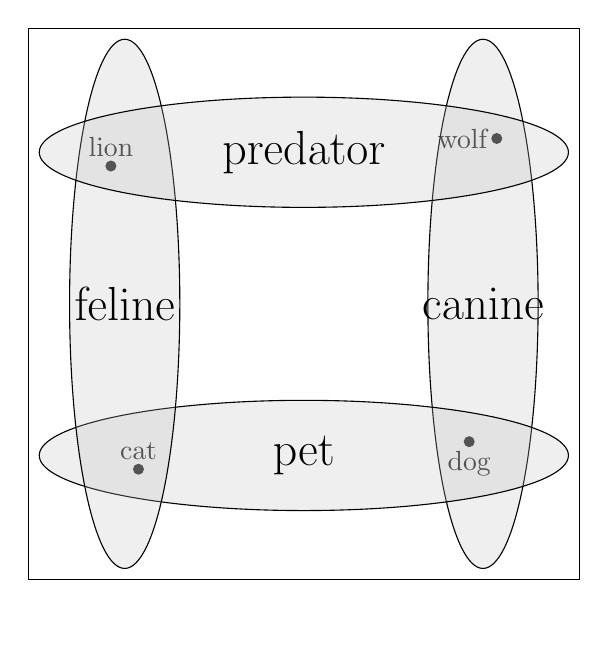
\begin{tikzpicture}[scale=0.07,baseline]
		\draw (0,0)--(-100,0)--(-100,-100)--(0,-100)--(0,0);
    	\draw (-15,-20) [left] node {wolf};
        \fill (-15,-20) circle[radius=1];
        \draw (-20,-75) [below] node {dog};
        \fill (-20,-75) circle[radius=1];
        \draw (-80,-80) [above] node {cat};
        \fill (-80,-80) circle[radius=1];
        \draw (-85,-25) [above] node {lion};
        \fill (-85,-25) circle[radius=1];
        \draw[fill=lightgray, fill opacity=0.25] (-17.5,-50) ellipse (10 and 48);
        \node at (-17.5,-50) {\LARGE canine};
        \draw[fill=lightgray, fill opacity=0.25] (-50,-77.5) ellipse (48 and 10);
        \node at (-50,-77.5) {\LARGE pet};
        \draw[fill=lightgray, fill opacity=0.25] (-82.5,-50) ellipse (10 and 48);
        \node at (-82.5,-50) {\LARGE feline};
        \draw[fill=lightgray, fill opacity=0.25] (-50,-22.5) ellipse (48 and 10);
        \node at (-50,-22.5) {\LARGE predator};
        \node at (-50,-102.5) [single arrow,draw,rotate=90,minimum height=40,minimum width=40,inner sep=15,opacity=0] {};
    \end{tikzpicture}
    \caption{a semantic space}
    \label{fig:bland}
    \end{subfigure}
    \begin{subfigure}[t]{0.5\textwidth}
    \centering
	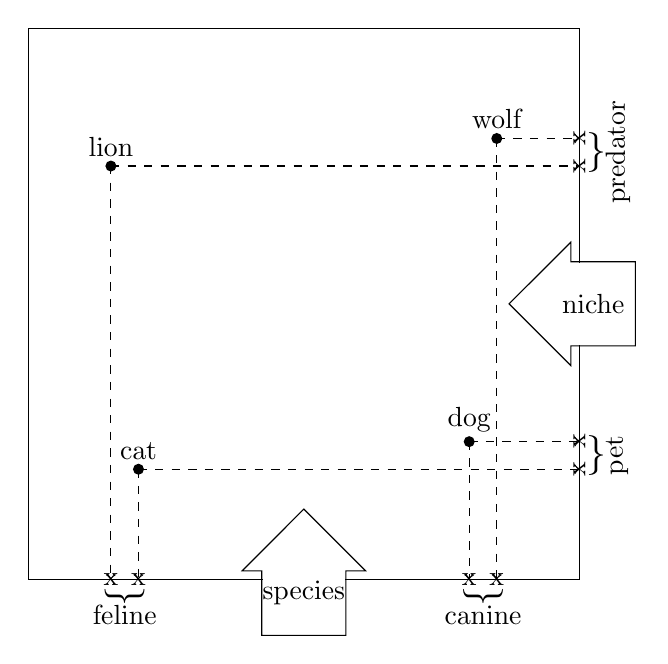
\begin{tikzpicture}[scale=0.07,baseline]
    	\draw (0,0)--(-100,0)--(-100,-100)--(-57.5,-100);
        \draw (-42.5,-100)--(0,-100)--(0,-57.5);
        \draw (0,-42.5)--(0,0);
    	\draw (-15,-20) [above] node {wolf};
        \fill (-15,-20) circle[radius=1];
        \draw[dashed,->] (-15,-20)--(-15,-100);
        \draw (-15,-100) node {x};
        \draw[dashed,->] (-15,-20)--(0,-20);
        \draw (0,-20) node [rotate=90] {x};
        
        \draw (-20,-75) [above] node {dog};
        \fill (-20,-75) circle[radius=1];
        \draw [dashed,->] (-20,-75)--(-20,-100);
        \draw (-20,-100) node {x};
        \draw [dashed,->] (-20,-75)--(0,-75);
        \draw (0,-75) node [rotate=90] {x};
        
        \draw (-80,-80) [above] node {cat};
        \fill (-80,-80) circle[radius=1];
        \draw [dashed,->] (-80,-80)--(-80,-100);
        \draw (-80,-100) node {x};
        \draw [dashed,->] (-80,-80)--(0,-80);
        \draw (0,-80) node [rotate=90] {x};
        
        \draw (-85,-25) [above] node {lion};
        \fill (-85,-25) circle[radius=1];
        \draw [dashed,->] (-85,-25)--(-85,-100);
        \draw (-85,-100) node {x};
        \draw [dashed,->] (-85,-25)--(0,-25);
        \draw (0,-25) node [rotate=90] {x};
        
        \node at (3,-22.5) [below,rotate=90] {predator};
        \node at (3,-22.5) {\Large\}};
		
        \node at (3,-77.5) [below,rotate=90] {pet};
        \node at (3,-77.5) {\Large\}};
		
        \node at (-17.5,-103) [below] {canine};
        \node at (-17.5,-103) [rotate=-90] {\Large\}};

        \node at (-82.5,-103) [below] {feline};
        \node at (-82.5,-103) [rotate=-90] {\Large\}};
        
        \node at (-50,-102.5) [single arrow,draw,rotate=90,minimum height=40,minimum width=40,inner sep=15] {};
        \node at (-50,-102.5) {species};
        \node at (2.5,-50) [single arrow,draw,rotate=180,,minimum height=40,minimum width=40,inner sep=15] {};
        \node at (2.5,-50) {niche};
    \end{tikzpicture}
    \caption{a contextual projection}
    \label{fig:reduce}
    \end{subfigure}
  \caption[Perspectives on Conceptual Categories]{In the two-dimensional space depicted in (a), the conceptual vagary of four words maps to overlapping, elongated and indeterminate spaces.  In (b), two different perspectives on the lexical space, represented by the arrows labelled \emph{niche} and \emph{species}, offer contextualised projections in one-dimensional clusters which remit conceptual clarity.}
\label{fig:perspective}
\end{figure}

Furthermore, the high dimensionality of vector space models of distributional semantics in particular should afford precisely these types of contextual viewpoints on potential relationships between words.  Rather than depending on \emph{a priori} disambiguation based on clustering or observations of context in the form of existing combinations of words, I propose that a technique for defining semantic subspaces \emph{in situ} will capture the momentary and situated way in which concepts come about in the course of a cognitive agent's entanglement with the world.  The way that relationships between words coalesce and then dissolve as we change our perspective on the base space of this model is designed to reflect the way that concepts emerge dynamically in response to unfolding events in the world, and the ability to selectively specify the dimensional profile of a space of geometrically related semantic representations should enable just this kind of shifting of conceptual perspective.  The theoretical mechanisms for making choices about multi-dimensional perspectives in semantic spaces will be discussed in the next section.

\paragraph{A Note on \emph{Context}} The term \emph{context} has been used widely and varyingly by authors in both theoretical and computational linguistics, and with good reason, as various senses of the concept of context are clearly at play in any serious discussion of the interplay between language and cognition.  Statistically minded computational linguists in particular, of whom I would like to count myself as one, have often used \emph{context} to refer to the window of co-occurrence in which a word token is observed within a sample of text.  In his description of a co-occurrence statistic for measuring semantic similarity, \cite{Schutze1992b} introduced the term \emph{context space} to refer to a space of co-occurrence dimensions, a terminology subsequently adopted by \cite{BurgessEA1997} in relation to their HAL system.  This notion of proximity within a text as context has persevered in the natural language processing literature.

Theoretical linguists and cognitive scientists, on the other hand, have tended to treat \emph{context} as a much more general condition wrapped up with the entire perceptual, phenomenological aspect of existing as a cognitive agent in a complex world.  So for instance \citeauthor{Bateson1972} says that ``message material, or information, comes out of a context into a context,'' \cite[][p. 404]{Bateson1972}, meaning that there is an alignment between the inner context of an agent and the outer context of the world, while \citepos{Grice1975} notion of \emph{implicature} holds that meaning is somehow always determined in a context, with the exact nature of context remaining somewhat open-ended, and this nomenclature has been carried on by subsequent researchers interested in the idea that cognition, conceptualisation, and, correspondingly, language are always in some way specified by a situation in the world.  The idea is that context is probably something that exists in large part outside of language, and almost certainly outside the informationally restrictive confines of word co-occurrences within a sentence.

\cite{MillerEA1991} address this definitional vagary in the context of early work on distributional semantics, and specifically opt to use context to refer to the co-occurrences that occur on a purely lexical and sentential level.  In my thesis, which seeks to address both those components of language measurable by an information processing system and the more general question of meaning as an environmentally situated phenomenon, I will endeavour to use the term \emph{context} strictly in reference to the latter notion of the situation in which concepts and semantics emerge in tandem.  With regard to words observed in proximity to one another, on the other hand, I will refer to \emph{co-occurrence}, and so additionally to a \emph{co-occurrence window} within which such observations are made and correspondingly a \emph{co-occurrence statistic} as a measure of the relative frequency of such observations.  Hopefully this terminological committment will serve to avoid confusion.

\section{Literal Dimensions of Co-Occurrence} \label{sec:litdims}
The model presented here is grounded within the paradigm of distributional semantics, which means that the conceptual geometries that it constructs are the product of observations of word co-occurrences in a large-scale corpus of textual data represented statistically.  Two procedurally distinct methodological regimens have emerged from the recent study of distributional semantics.  The first, and more established, approach involves tabulating word co-occurrence frequencies and then using some function over these to build up word-vector representations.  With roots in the frequentist analysis described by \cite{SaltonEA1975}, recent research has typically involved matrix factorisation techniques presented as either (or both) an optimisation method \citep{BullinariaEA2012} or a noise reducing mechanism \citep{KielaEA2014}.\footnote{\cite{BullinariaEA2012}, \cite{LapesaEA2013}, and \cite{KielaEA2014} have all reported that dimensional reduction techniques including SVD, random indexing, and top frequency feature selection generally do not improve results on word similarity and composition tests, with some notable parameter and task specific exceptions.}  A more recent approach, which has received a great deal of attention with the increasing availability of large-scale data and the corresponding advent of complex neural network architectures, involves using machine learning techniques to iteratively learn word-vector representations in an online, stepwise traversal of a corpus \citep{BengioEA2003,CollobertEA2008,KalchbrennerEA2014}.

Another important similarity between these two approaches is that they each in their own way move towards a representation of relationships between word-vectors which is to some extent optimally informative, and, by the same token, abstract.  In the instance of neural network approaches, this is clearly the case due to the nature of the technique: the dimensions of this variety of model exist as basically arbitrary handles for gradually adjusting the relative positions of vectors, slightly altering every dimension of each vector each time the corresponding word is observed in the corpus.  And, as far as models based on explicit co-occurrence counts are concerned, the favoured technique tends to involve starting with a large, sparse space of raw co-occurrence statistics (frequencies, or, more typically, an information theoretic type metric) and then factorising this matrix using a linear algebraic technique such as singular value decomposition.  The result, in either case, is a space of vectors which exists just for the sake of placing words in a relationship where distance corresponds to a semantic property, consisting of dimensions which can only be interpreted in terms of the way that they allow the model to relate words, not in terms of their relationship to the underlying data.

A key feature of the methodology proposed in this thesis is that it maintains a base space of highly sparse co-occurrence statistics, which, despite their anchoring in the relatively abstract realm of word positions in a digitised corpus, I will describe as \emph{literal} in the sense that they can be interpreted as corresponding to actual relationships between word tokens in the world.  As mentioned in the previous section, a fundamental objective of this methodology is to afford an abundance of potential perspectives on co-occurrence data.  This objective is accomplished by providing a model with a corresponding proliferation of dimensions from which to make projections by way of context specific selections of subsets of dimensions.  Furthermore, by maintaining the literal connection between the dimensions and the underlying data, the methodology likewise sustains a mechanism for selecting the dimensions in a way that is fundamentally interpretable, in that we can predict something about the geometric contribution of a given dimension to a subspace based on the types of words which tend to co-occur with that dimension.  The co-occurrence profiles of the dimensions themselves will become an important criterion for dimensional selection, and having a very large set of such profiles to analyse will give a semantic model great scope in its capacity for adopting situational perspectives on the relationships between words.

%I don't wish to claim that there is scope for completely or even mainly recapitulating a nuanced conceptual model from the data available in a purely textual environment; to do so would be to move towards claims that intentionality can emerge from rule-based operations on symbols, and the problems with this have been explored by \citepos{Searle1980} Chinese room argument and a subsequent generation of philosophers \citep{PrestonEA2002}.  But I would like to suggest that by building a base model that maintains the accessibility of unreduced co-occurrence information, we likewise maintain the ability to manipulate this base model extemporaneously, in reaction to the ongoing emergence of new contextual information.  The idea is that such a base model would essentially represent the superset of all possible dimensions available for \emph{ad hoc} selection in the course of a 

So the proper framework for describing the model to be examined in this thesis is not so much a single space of word-vectors as a lattice consisting of the power set of all possible combinations of the dimensions characterising the base space.  At the top of this lattice -- the \emph{join} -- sits a single $d$-dimensional space consisting of every available one of the $d$ co-occurrence terms observed throughout the underlying corpus, \revJB{14}{and here a \emph{co-occurrence term} refers to the words that, through their observation in the proximity of target words across the corpus, are being selected as a basis for examining and comparing word vectors within a particular context (this model parameter will be explained in more detail in Chapter~\ref{sec:project})}.  At the bottom of the lattice -- the \emph{meet} -- sit $d$ different one-dimensional spaces, each space corresponding to a single co-occurrence term.  If the meet is considered layer-$1$ of the lattice, and the join is considered layer-$d$, then any given interstitial layer-$j$ consists of every possible combination of $j$ dimensions of co-occurrence statistics.  A diagram of a very simple example of one such model is presented in Figure~\ref{fig:lattice}, illustrating the possible subspaces projected from a vastly simplified model consisting of just three co-occurrence dimensions (these particular spaces will be explored in the next section, providing the basis for the interpretable geometries illustrated in Figure~\ref{fig:instruments}).

\begin{figure}
\centering
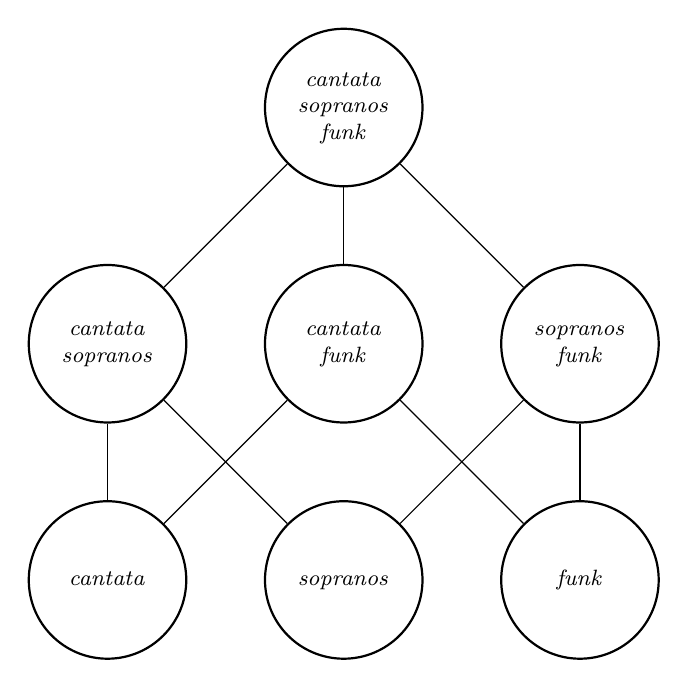
\begin{tikzpicture}[node distance=3cm,every node/.style={draw=black,thick,circle,inner sep=0pt}]
  \footnotesize
  \node[minimum size=2cm](join) {\begin{tabular}{c}
    \emph{cantata} \\
    \emph{sopranos} \\
    \emph{funk}
  \end{tabular}};
  \node[minimum size=2cm](two2) [below of=join] {\begin{tabular}{c}
    \emph{cantata} \\
    \emph{funk}
  \end{tabular}};
  \node[minimum size=2cm](two1) [left of=two2] {\begin{tabular}{c}
    \emph{cantata} \\
    \emph{sopranos}
  \end{tabular}};
    \node[minimum size=2cm](two3) [right of=two2] {\begin{tabular}{c}
    \emph{sopranos} \\
    \emph{funk}
  \end{tabular}};
  \node[minimum size=2cm](one2) [below of=two2] {\begin{tabular}{c}
    \emph{sopranos}
  \end{tabular}};
  \node[minimum size=2cm](one1) [left of=one2] {\begin{tabular}{c}
    \emph{cantata}
  \end{tabular}};
  \node[minimum size=2cm](one3) [right of=one2] {\begin{tabular}{c}
    \emph{funk}
  \end{tabular}};
  \draw (two1)--(join);
  \draw (two2)--(join);
  \draw (two3)--(join);
  \draw (one1)--(two1);
  \draw (one1)--(two2);
  \draw (one2)--(two1);
  \draw (one2)--(two3);
  \draw (one3)--(two2);
  \draw (one3)--(two3);
\end{tikzpicture}
\caption[A Lattice of Co-Occurrence Dimensions]{A lattice of three dimensions, including the two-dimensional subspaces which are used for analysing the conceptual geometry of a small set of word-vectors in Figure~\ref{fig:instruments}.  \revJB{14}{The dimension labels correspond to words observed to co-occur with the words that will be analysed in this space in a way that generates a particular conceptual geometry.}}
\label{fig:lattice}
\end{figure}

An important distinction must be drawn, however, between the representation of my model as a lattice and the use of manifolds as an inferential mechanism.  Formal concept analysis in particular has made a productive discipline out of applying lattice type structures to conceptual modelling, using the semi-hierarchical properties of lattices to capture logical relationships of entailment \citep{Wille1982}.  That body of work takes as given that concepts are ``the basic units of thought formed in dynamic processes within social and cultural environments,'' \citep[][p. 2]{Wille2005}.  \cite{Widdows2004} offers a broad overview of how this approach might be pursued through corpus linguistic techniques, while \cite{GeffetEA2005} and, more recently, \cite{KartsaklisEA2016} have proposed statistical techniques using \emph{feature inclusion} metrics to assess the potential entailment relationships between candidate words and corresponding concepts.  The assumption inherent in this interesting work is that words are in some sense supervenient upon the concepts they denote, and that the statistical features of a language will by and large recapitulate the conceptual structure upon which it sits.

As \cite{Rimell2014} has pointed out, however, it is problematic to assume that a spectrum of co-occurrence alone can indicate relationships of hyponymy and hypernymy.  It stands to reason, for instance, that a word with a taxonomically specific denotation such as \emph{bulldog} should probably have a co-occurrence profile including words omitted from the corresponding profile of a word like \emph{lifeform}, which has an ostensibly more general extension---even excluding some of the ambiguity inherent in \emph{bulldog}, it seems reasonable to talk about a \emph{pet bulldog} but less so to talk about a \emph{pet lifeform}, for instance.  Rimell has proposed a measure of change in \emph{topic coherence} as word-vectors are combined algebraically in order to detect entailment relationships.  This measuring is achieved specifically through a process of dimension-by-dimensions comparison between potentially related word-vectors, in particular the \emph{vector negation} method described by \cite{Widdows2003}, combined with topic modelling techniques to analyse the coherence of features distilled by the selectional process.

The methodology proposed in this thesis adheres to the same principle of fine-grained cross-dimensional analysis described by Rimell.  In addition to the practical issues raised by Rimell, my approach is also designed to remain pointedly uncommitted to any claim that concepts are atomic or elementary to thought, or that language and concepts are involved in any kind of strictly hierarchical interrelationship.  Instead, my models operate through an analytical traversal of lattices of subspaces in search of combinations of dimensions that capture conceptually \emph{salient} profiles of co-occurrence features.  If a consequence of this stance is that a model built from this methodology can't be understood in terms of nested, ordered relationships, though, then the question of how conceptual relationships do emerge situationally from the methodology remains.  The next section of this theoretical overview will examine how the actual geometry of a projected subspace itself is expected to do this conceptual work.

\section{Interpretable Geometry} \label{sec:interpretable}
It is important at this point to distinguish between two different modes of interpretability at play within the operation of the methodology I'm proposing.  On the one hand, we have the process for selecting subspaces described above: this process requires a model composed of tractable dimensions of statistics that can be interpreted based on expectations generated from an analysis of some sort of contextually relevant information.  Some specific mechanisms for this process will be discussed in the next chapter.  Then on the other hand, once this selectional process has taken place, we find ourselves with a subset of dimensions defining a specific subspace.  My claim is that, given the correct selectional criteria for performing this projection -- this traversal of our lattice of vector spaces -- we should be able to generate a subspace in which the projected word-vectors will be interpretable in terms of the actual geometric features of this subspace.

The idea of exploiting the geometry of a transformed space of word statistics is not new.  Indeed, seminal work on latent semantic analysis was motivated by precisely the insight that a singular value decomposition of a high-dimensional, sparse matrix of statistical data about word co-occurrences would result in a dense lower dimensional matrix in which dimensions characterise \emph{latent semantics} rather than literal word co-occurrences \citep{DeerwesterEA1990}.  Thus the linear algebraic methodology of generating a lower dimensional matrix of optimally informative dimensions arguably transforms a space of specific co-occurrence tendencies into a space of more general conceptual relationships.  In fact, \citeauthor{LandauerEA1997} have subsequently argued that the dimensional reduction by way of factorisation itself might directly mirror cognitive conditioning, modelling the way that the mind can ``correctly infer indirect similarity relations only implicit in the temporal correlations of experience,'' \citep[][p. 212]{LandauerEA1997}.

Of course the dimensions of a factorised matrix are still not interpretable in themselves.  They are, rather, an optimal abstraction of the underlying data, in which each dimension is maximally informative -- and, accordingly, orthogonal -- in comparison to the other dimensions.  What we desire in a model, however, is a mechanism for actually interpreting directions and regions within a subspace projected by the model.  This objective is motivated by \citepos{Gardenfors2000} insight into the inferential power of \emph{conceptual spaces}: by building spaces in which the dimensions themselves correspond to \emph{properties}, G\"{a}rdenfors has illustrated how features of points and regions within these spaces such as convexity and betweeness can be interpreted as corresponding to conceptual membership and can accordingly be used to reason about relationships between concepts.  In more recent work, motivated by psycholinguistic insight into the significance of the \emph{intersubjectivity} by which language facilitates the mutual ascription of cognitive content between interlocutors, \cite{Gardenfors2014} has proposed that semantics are derived from a communicative alignment of conceptual spaces.

A classic example of a G\"{a}rdenforsian conceptual space is the space of colours, which can be defined in terms of, for instance, hue, brightness, lightness, and colourfulness: any colour percept can be specified as a point corresponding to coordinates along each of these dimensions.  Moreover, regions within the space of colours can be defined geometrically: the concept \textsc{red} will correspond to a convex region within the space, and any point lying between two points known to be labelled \emph{red} will likewise be considered \textsc{red}.  \cite{Jager2010} has devised an experiment mapping linguistic descriptions to conceptual regions precisely within the domain of colours.  Taking a large set of multi-lingual data regarding colour naming conventions and treating each of 330 different colours as an initially independent dimension, J\"{a}ger demonstrated how an extrapolation of optimally informational dimensions via a principle component analysis revealed clusterings of colour names into convex regions.\footnote{The cross-cultural universality of colour naming conventions presented by \cite{KayEA1999}, which J\"{a}ger takes as a basis for his research, is controversial to say the least -- see \cite{Levinson2001} for an alternative point of view -- but J\"{a}ger's work remains a good example of a computational technique for extrapolating conceptual spaces from quantitative linguistic data.}

Similarly motivated by G\"{a}rdenfors's model of conceptual spaces, \cite{DerracEA2015} have built vectors of domain specific documents, associating word frequencies within documents with document labels.  A multi-dimensional scaling procedure is then used to project these document-vectors into a Euclidean space in which the authors predict that properties such as \emph{parallelness} and \emph{betweeness} will correspond to conceptual relationships between documents.  The authors demonstrate that geometry in their projected spaces does indeed afford conceptual interpretation: the vector they construct from large scale textual data for the word \emph{bog} is found to be more or less between the vectors for \emph{heath} and \emph{wetland}, for instance, and the vector for the film \emph{Jurassic Park} lies in directions associated with \textsc{dinosaurs} and \textsc{special effects}.  This work is particularly notable in that \citeauthor{DerracEA2015} appreciate the significance of projecting spaces which are interpretable in terms of Euclidean distances rather than simply the cosine similarity of vectors extending from the origin of a space: Euclidean metrics provide a platform for more nuanced considerations of the relationships between points.

The type of space exemplified by the research of J\"{a}ger and \citeauthor{DerracEA2015} is moving towards being a conceptual space in the way that its geometry offers itself up to semantic interpretation, but importantly these remain static spaces comprised of abstract dimensions, albeit dimensions generated in order to optimise the interpretability of the spaces they delineate.  The objective of my model is to emulate the geometric interpretability of these other spaces in an extemporaneous, contextually dynamic way.  To illustrate this point, consider the two spaces illustrated in Figure~\ref{fig:instruments} (taken from real co-occurrence data, as described in the next chapter, and based on the lattice of subspaces illustrated in Figure~\ref{fig:lattice}).  Here co-occurrence statistics are used to define three different dimensions, from which two different two-dimensional subspaces are selected with word-vectors plotted into each subspace.  In each subspace, a particular conceptual geometry emerges, oblique to the axes of each subspace but nonetheless indicating distinct conceptual regions in which words align themselves in an interpretable way.

\begin{figure}[t]
	\begin{subfigure}[t]{0.5\textwidth}
    \centering
	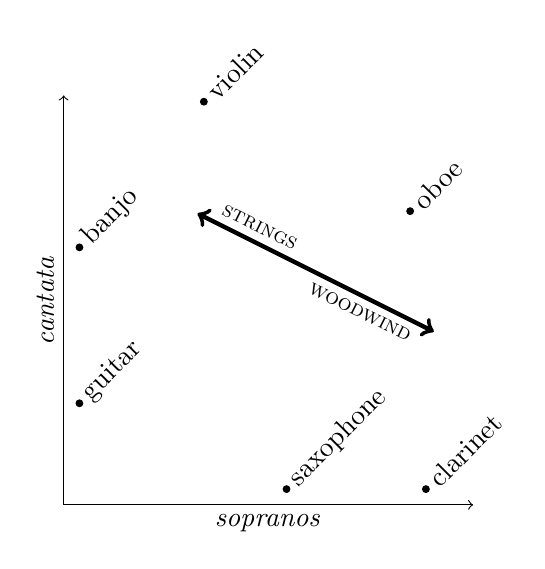
\begin{tikzpicture}[scale=1,baseline]
		\draw [->] (-0.2,-0.2)--(5,-0.2);
		\draw [->] (-0.2,-0.2)--(-0.2,5);
		\node at (2.4,-0.2) [below] {\emph{sopranos}};
		\node at (-0.2,2.4) [above,rotate=90] {\emph{cantata}};
		\draw [<->,ultra thick] (1.5,3.5)--(4.5,2);
		\node at (2.2,3.15) [above,rotate=-26.57] {\footnotesize \textsc{strings}};
		\node at (3.65,2.425) [below,rotate=-26.57] {\footnotesize \textsc{woodwind}};
		\node at (0.0,1.09) [right,rotate=45] {guitar};
		\fill (0.0,1.09) circle[radius=0.05];
		\node at (0.0,3.07) [right,rotate=45] {banjo};
		\fill (0.0,3.07) circle[radius=0.05];
		\node at (1.58,4.92) [right,rotate=45] {violin};
		\fill (1.58,4.92) circle[radius=0.05];
		\node at (2.63,0.0) [right,rotate=45] {saxophone};
		\fill (2.63,0.0) circle[radius=0.05];
		\node at (4.40,0.0) [right,rotate=45] {clarinet};
		\fill (4.40,0.0) circle[radius=0.05];
		\node at (4.20,3.53) [right,rotate=45] {oboe};
		\fill (4.20,3.53) circle[radius=0.05];
    \end{tikzpicture}
    \caption{\textsc{strings} vs \textsc{woodwind}}
    \label{fig:svsw}
    \end{subfigure}
    \begin{subfigure}[t]{0.5\textwidth}
    \centering
	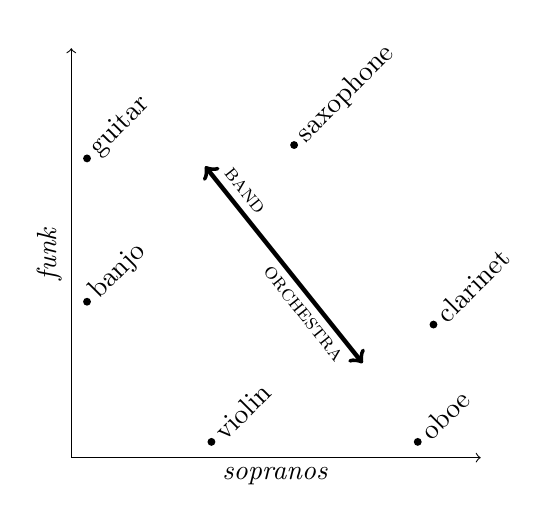
\begin{tikzpicture}[scale=1,baseline]
		\draw [->] (-0.2,-0.2)--(5,-0.2);
		\draw [->] (-0.2,-0.2)--(-0.2,5);
		\node at (2.4,-0.2) [below] {\emph{sopranos}};
		\node at (-0.2,2.4) [above,rotate=90] {\emph{funk}};
		\draw [<->,ultra thick] (1.5,3.5)--(3.5,1);
		\node at (1.85,3.0625) [above,rotate=-51.35] {\footnotesize \textsc{band}};
		\node at (2.9,1.75) [below,rotate=-51.35] {\footnotesize \textsc{orchestra}};
		\node at (0.0,3.60) [right,rotate=45] {guitar};
		\fill (0.0,3.60) circle[radius=0.05];
		\node at (0.0,1.78) [right,rotate=45] {banjo};
		\fill (0.0,1.78) circle[radius=0.05];
		\node at (1.58,0.0) [right,rotate=45] {violin};
		\fill (1.58,0.0) circle[radius=0.05];
		\node at (2.63,3.77) [right,rotate=45] {saxophone};
		\fill (2.63,3.77) circle[radius=0.05];
		\node at (4.40,1.49) [right,rotate=45] {clarinet};
		\fill (4.40,1.49) circle[radius=0.05];
		\node at (4.20,0.0) [right,rotate=45] {oboe};
		\fill (4.20,0.0) circle[radius=0.05];
    \end{tikzpicture}
    \caption{\textsc{band} vs \textsc{orchestra}}
    \label{fig:bvso}
    \end{subfigure}
  \caption[Conceptual Directions in a Semantic Space]{Based on real co-occurrence data, swapping one dimension in a two-dimensional subspace reveals two different conceptual geometries.}
  \label{fig:instruments}
\end{figure}

The first thing to note about these spaces is the way that swapping a single dimension in a two dimensional subspace can have a significant impact on the conceptual affordances of the subspace's geometry.  Realigning the relationships between terms along a single axis leads to a complete shift in the groupings of terms, and, correspondingly, to a shift in the interpretation of regions and directions.  If these are conceptually sound subspaces, then we might expect word-vectors found within the area of the triangle described by the points labelled \emph{guitar}, \emph{banjo}, and \emph{violin} in Figure~\ref{fig:svsw} to be the names of other string instruments, or other conceptually relevant terms.  This is possibly asking too much of a subspace consisting of data regarding co-occurrences with just two terms across a large scale corpus, but as we scale up the dimensionality of the space -- as we ascend the lattice of subspaces of a fully realised model -- we can expect proper conceptual spaces to begin to coalesce.

The next thing to note is that the dimensions themselves are not especially interpretable.  While these dimensional profiles are explicable -- and indeed the ability to trace these statistics back to the corpus might turn out to be a desirable property for some applications -- the dimensions themselves do not conform to \citepos{Gardenfors2000} notion of dimensions as representing the properties that compose a concept.  It might be surprising, for instance, that the word \emph{cantata} has a higher propensity for co-occurrence with the word \emph{banjo} than with the word \emph{clarinet}, given that cantatas have traditionally included parts for the latter but not the former.  However, an examination of the underlying data, extracted, as described in the next chapter, from English language Wikipedia, reveals that the term \emph{cantata} has been adopted, perhaps somewhat figuratively, by some bluegrass musicians, and so co-occurrences with \emph{banjo} are indeed observed.

Rather than consider such usage as anomalous or attempt some sort of \emph{a priori} word sense disambiguation, I propose to embrace the haphazardness of language and use it as a tool for projecting conceptually productive geometries.  In fact it would be surprising if it turned out that in anything other than the most specialised cases we could simply pick dimensions based on their labels and then expect co-occurrence statistics to play out in a conceptually coherent way, as this would contradict the relevance theoretic thesis that language in use is always significantly underspecified.  With this in mind, I suggest that we consider some set of dimensions, delineating a subspace and the corresponding geometry of word-vectors, to map precisely to a given context, and to effectively serve as the connective structure between language and conceptualisation.  Under this regimen, the dimensions themselves become the constitutive substance of a context, but they do not compositionally define any context in which they participate; rather, the contextualisation is an emergent property of the combination of dimensions underwriting it, corresponding to \emph{a way of speaking} about things.

The spaces illustrated in Figure~\ref{fig:instruments} are the product of a survey of a lattice consisting of combinations of just three dimensions, and as such the conceptual affordances of this toy model are highly limited.  As we add dimensionality to the model, however -- as we observe more terms co-occurring with our vocabulary of word-vectors -- we can expect an exponential growth in the combinatory possibilities of subspace construction.  With enough dimensions from which to choose, and with an appreciable degree of variance between the profiles of each dimensions, there should be scope for projecting more or less any constellation of word-vectors we desire.  The next question, then, is how to go about actually extracting a high dimensional base model of co-occurrence statistics from a large scale textual corpus and then exploring the conceptual possibilities of this base space's inherent subspaces.  The next chapter will answer this question.

%\section{A Computational Process}
%In this final section of this chapter, a technical implementation of the model described throughout the preceding three sections will be explained in detail.

%\subsection{A Large Scale Textual Corpus}
%The first step in a corpus based approach to natural language processing is the selection of the data which will provide the basis for our model.  I've picked the English language portion of Wikipedia as my data source, a choice which is in accordance with a good deal of work done in the field.  Some authors 

%In the case of the model used throughout this thesis, the November 2014 dump of English language Wikipedia has been used.\footnote{Accessible at XXX}  A data cleaning process has been implemented, the first step of which is the chunking of the corpus into individual sentences.  Next parenthetical phrases are removed from each sentence, as these can potentially skew co-occurrence data, and all other punctuation is subsequently removed.  All characters are converted into lowercase to avoid words capitalised at the beginning of sentences, quotations, and other places from being considered as unique types.  Finally, the articles \emph{a}, \emph{an}, and \emph{the} are removed as they can distort co-occurrence windows (consider, for instance, how these terms affect the proximity of the other words in the phrase ``a mouse, an owl, and a dog sat on the moon'').  The cleaned corpus contains about

%-WORD, SENTENCE COUNTS

%As is generally the case with data cleaning, these measures are prone to error: for instance, due to the removal of punctuation, the contraction \emph{we're} will be considered identical to the word \emph{were}.  One of the strengths of the subspace projection technique that my model uses is its resilience to noise.  So, for instance, misspellings will be categorised as highly anomalous co-occurrence dimensions and are therefore unlikely to be contextually selected -- or, if they are regularly encountered enough to be contextually significant, there may well be useful information in the co-occurrence profile of such mistakes -- and essentially ubiquitous words are unlikely to provide context specific information, so the ambiguity between \emph{we're} and \emph{were} is unlikely to be drawn into any of the subspaces actually projected by the model.

%From the cleaned corpus, the model's vocabulary is defined as the top 200,000 most frequently occurring word types.  This cut-off point is very close to the point where the total number of word tokens included -- that is, occurrences of any word of any type -- included by selecting all instances of all vocabulary words equals the total number of word types -- that is, unique word forms -- excluded.  Given the Zipfian distribution of word frequencies as observed throughout the corpus, this means that more than 95\% of the co-occurrence data available from the corpus will be taken into account by the model, while the number of word-vectors used to express this data represents less than 5\% of the potential vocabulary---a fairly efficient way of extrapolating statistics from the corpus.

%- human vocabulary size

%\subsection{Mutual Information of Word Co-Occurrences}
%The critical event in the 

%Here, following the example of almost all distributional semantic work, co-occurrence between a word $w$ and another word $c$ will be considered in terms of the number of other words between $w$ and $c$.  In the case of my model, again in accord with the a great deal of work within the field, a statistic for word $w$ in terms of its co-occurrence with $c$ will be derived from the consideration of all the times that $c$ is observed within $k$ words of $w$, where $k$ is one of the primary model parameters that will be considered in the experiments reported in later chapters of this thesis.  Based on these co-occurrence events, a matrix $M$ is defined, where rows consist of word-vectors, one for each of the 200,000 words in the vocabulary, and columns correspond to terms with which these vocabulary words co-occur.  These column-wise co-occurrence dimensions include the words in the vocabulary, including the possible co-occurrence of a word with itself (``a \emph{rose} is a \emph{rose} is a \emph{rose}'', for instance) as well as many, many words that are not in the vocabulary, to the extent that every word type in the corpus is considered as a dimension of co-occurrence.

%In this last respect, my model diverges from the typical approach, which usually seeks to limit not only the vocabulary but also the dimensionality of the underlying co-occurrence matrix.  This has typically involved a curtailing of the number of co-occurrence terms at both ends of the frequency spectrum, based on the assumption that both high frequency so-called function words (the prepositions, conjunctions, and so forth) and low frequency terms such as obscure proper names will muddy a model with either general flattening or highly topical skewing.  In the case of my model, however, these problems are irrelevant, as dimensions will be selected on a case-by-case, context specific basis, and there is no good reason to discard information which may in some possibly unforeseen circumstance prove relevant.  The result is a 200,00 by $\approx$ 7.5 million matrix $M$ where a scalar corresponding to co-occurrences between $w$ and $c$ is defined in terms of this equation:

%\begin{equation}\label{eq:MI}
%M_{w,c} = \log_2 \left(\frac{n_{w,c} \times W}{n_w \times \left(n_c + a\right)} + 1\right)
%\end{equation}

%Here $n_{w,c}$ represents the total number of times that that $c$ is observed as co-occurring in a sentence within $k$ words on either side of $w$, $n_w$ is the independent frequency of occurrences of $w$, and $c$ is likewise the overall frequency of $c$ being observed as a co-occurrence term throughout the corpus.  $W$ is the overall occurrence of all words throughout the corpus---and it should be noted that, excluding the term $a$, the ratio in Equation~\ref{eq:MI} is equivalent to the joint probability of $w$ and $c$ co-occurring.  The application of a logarithm to this ratio, again a common practice, is in the spirit of \citepos{Shannon} information theory, and is 

%The term $a$ is a skewing constant used to prevent highly specific co-occurrences from dominating the analysis of a word's profile, set for the purposes of the work reported here at 10,000.\footnote{Anecdotally, the first combination of input words analysed during an early stage of the development of this model that didn't use a smoothing constant was the phrase ``musical creativity'', and the very first dimension indicated by the analysis was labelled \emph{gwiggins}---my primary supervisor's email handle.  Prof. Wiggins's deep connection with music and creativity meant that every instance of \emph{gwiggins} occurring throughout Wikipedia was in the vicinity of both \emph{musical} and \emph{creativity}, and so the dimension was indicated by the combination of these terms, which makes sense, but it was still a bit eerie to have such a personally relevant result generated by a model based on such general data.}

%Finally, the entire ratio is skewed by 1 so that all values returned by the logarithm will be greater than 0, with a value of zero therefore indicating that two words have never been observed to co-occur with one another.  This is again a departure from standard practice, where, in word counting models, a \emph{pointwise mutual information} mechanism involving not skewing the ratio and instead treating any ratio of frequencies less than 1 -- that is, any co-occurrence that is observed less than often than balance of the mean values for all occurrences of $w$ and all co-occurrences with $c$ -- as being equivalent to 0, or no co-occurrence at all.  The motivation for this more typical technique is again to avoid incorporating unnecessary and potentially confounding information into a model, but, again, in the case of my model, the dimensional selection process will tend to ignore such information, and at the same time, as will be seen, data regarding relatively unlikely co-occurrences can sometimes also be quite informative.  In support of my technique, it is worth mentioning that the vast majority of potential co-occurrences will never be observed, and, at the same time, a comprehensive language model should maintain at least the possibility of any co-occurrence

%\cite{Brown}

%so there seems to be wisdom in the idea of not throwing away information about even relatively unlikely linguistic events.

%\subsection{Dimensional Selection Techniques}
%Having established a base model of co-occurrence statistics, the 

%\begin{equation}\label{eq:oldNorm}
%w^j_i = \frac{w^j_i}{\sqrt{\sum_{k=1}^{b} \left(w^k_i\right)^2}}
%\end{equation}

%\begin{equation}\label{eq:Norm}
%w^j_i = \frac{w^j_i}{\sum_{k=1}^{b} abs\left(w^k_i\right)}
%\end{equation}

%\begin{equation}\label{eq:Arg}
%\mu_c =  \frac{1}{n} \sum_{w=1}^{n}N_{w,c}
%\end{equation}

%\begin{equation}\label{eq:Trans}
%M_{w,c} \Rightarrow S_{w,c'}
%\end{equation}
%\subsection{Extracting Semantics from Geometric Features}

\chapter{Context Sensitive Distributional Semantics} \label{chap:method}
In the previous chapter, I laid down the theoretical groundwork for a distributional semantic methodology for dynamically establishing perspectives on statistical data about language use.  In this chapter, I'll describe the technical details for building a computational implementation of such a methodology.  The objective of this implementation is to establish a rigorous procedure for generating subspaces of word-vectors, based on observations of word co-occurrences in an underlying corpus, the geometries of which are semantically productive in particular contexts.  This will involve three steps:

\begin{enumerate}
\item The selection, processing, and analysis of a large scale textual corpus in order to create a high dimensional base space of co-occurrence statistics;
\item The development of techniques for selecting lower dimensional subspaces based on some sort of contextualising input;
\item The exploration of the geometry of the projected subspaces in search of semantic correlates.
\end{enumerate}

The following three sections will pursue each of these aspects of a technical implementation in turn.  The end result is effectively a mapping from text as raw data to geometry as semantic generator.  A fourth section offer a mathematical consideration of how the geometries of contextualised subspaces provide a basis for either testing or producing probabilistic hypotheses about word co-occurrences.  The fifth section will describe an alternative, general interpretation of the statistical data which underwrites my models and additionally offer a brief overview of another distributional semantic methodology, both to be used as a point of comparison in the empirical results which will be discussed in subsequent chapters.  Finally, the sixth section will offer a proof of concept by way of a small, purpose-built experiment involving the reconstruction of a lexical taxonomy.

\section{Establishing and Analysing a Large Scale Corpus} \label{sec:pmi}
The first step in a corpus based approach to natural language processing is the selection of the data which will provide the basis for our model.  I've picked the English language portion of Wikipedia as my data source, a choice which is in accordance with a good deal of work done in the field.  For instance, \cite{GabrilovichEA2007} and \cite{CollobertEA2008}, to name just a couple, use Wikipedia as their base data for training distributional semantic models designed to perform tasks similar to the ones explored in subsequent chapters, while \cite{BaroniEA2014}, \cite{PenningtonEA2014}, and \cite{GutierrezEA2016} use amalgamated corpora that include Wikipedia as a major component.  Wikipedia provides a very large sample of highly regular language, meaning that we can expect a certain syntactic and semantic consistency as well as language which, if not always overtly literal, is likewise not typically abstruse or periphrastic.  This should supply a source of linguistic data in which, to revisit the central dogma of the distributional hypothesis, words which occur in a particular syntactic and lexical setting can be expected to be semantically related.

In the case of my implementations, the November 2014 dump of English language Wikipedia has been used.\footnote{Relatively recent Wikipedia dumps are available at \url{https://dumps.wikimedia.org/}.}  A data cleaning process has been implemented \revAK{16}{using code written by me specifically for the development of my methodology}, the first step of which is the chunking of the corpus into individual sentences, ignoring headers, footers, captions, and labels.\footnote{\revAK{16}{All code involved in the construction of my models, from data cleaning through to the projection of semantically contextualised subspaces, can be found at \url{https://github.com/masteradamo/ModelMaker/}.}}  Next parenthetical phrases are removed from each sentence, as these can potentially skew co-occurrence data: \revJB{15}{as parentheses often serve to insert information somewhat outside the content of a sentence, they can also act to interupt the syntagmatic flow and corresponding data inherent in word proximity, as in the case of a sentence such as ``The old dog (an animal often noted for its friendliness towards humans) ate the bone'', so these potential interferences are simply eliminated.} \del{and all} All other punctuation other than hyphenation is subsequently removed.  All characters are converted into lowercase to avoid words capitalised at the beginning of sentences, quotations, and other places being considered as unique types.  Finally, the articles \emph{a}, \emph{an}, and \emph{the} are removed as they can distort co-occurrence distance counts, and then all sentences containing less than five words are discarded.  The cleaned corpus contains nearly 1.1 billion word tokens, consisting of almost 7.5 million unique word types spread across about 61 million sentences.  The distribution of these types is predictably Zipfian: over 10 million occurrences of each of the top nine word types are observed, while the least frequent 4.27 million words -- more than half of all types -- only occur once.  The top end of this distribution is populated by conjunctions, prepositions, and pronouns, while the bottom end is characterised by obscure place names, one-off abbreviations, unicode representing non-Latin alphabet terms, and a good many spelling errors.

As is generally the case with data cleaning, these measures are prone to error: for instance, due to the removal of punctuation, the contraction \emph{we're} will be considered identical to the word \emph{were}.  One of the strengths of the subspace projection technique that my methodology uses is its resilience to noise.  So, for instance, misspellings will be categorised as highly anomalous co-occurrence dimensions and are therefore unlikely to be contextually selected -- or, if they are encountered regularly enough to be contextually significant, there may well be useful information in the co-occurrence profile of such mistakes -- while, at the other end of the spectrum, essentially ubiquitous words are unlikely to provide context specific information, so the ambiguity between \emph{we're} and \emph{were} is unlikely to be drawn into any of the subspaces actually projected by the model.

From the cleaned corpus, a model's vocabulary is defined as the top 200,000 most frequently occurring word types.  This cut-off point is very close to the point where the rate of word tokens included by selecting all instances of all vocabulary words equals the rate of word types excluded.  Given the Zipfian distribution of word frequencies as observed throughout the corpus, this means that more than 95\% of the co-occurrence data available from the corpus will be taken into account by the model, while the number of word-vectors used to express this data represents less than 5\% of the potential vocabulary---a fairly efficient way of extrapolating statistics from the corpus.  The selection of this as a cut-off point means that the least frequent words in the vocabulary occur 83 times throughout the corpus.

Having processed the corpus and established the target vocabulary, the next step of this methodology is to build up a base space of co-occurrence statistics.  Here, following the example of many other distributional semantic models, co-occurrence between a word $w$ and another word $c$ will be considered in terms of the proximity of $c$ to $w$.  In the case of my methodology, and again in accord with a great deal of work within the field, a statistic for word $w$ in terms of its co-occurrence with $c$ will be derived from the consideration of all the times that $c$ is observed within $k$ words to either side of $w$ within the boundary of a sentence, where $k$ is one of the primary model parameters that will be considered in the experiments reported in later chapters of this thesis \revJB{13}{(the two values for $k$ that will be explored are 2 and 5, and so I will refer to $2x2$ and $5x5$ word co-occurrence windows in subsequent results)}.  \revAK{3}{These values have been selected to be in line with standard parameters reported in the literature; see} \cite{KielaEA2014} \revAK{3}{for a comprehensive review of the effects of window size.}

Based on these co-occurrence events, a matrix $M$ is defined, where rows consist of word-vectors, one for each of the 200,000 words in the vocabulary, and columns correspond to terms with which these vocabulary words co-occur.  These column-wise co-occurrence dimensions include the words in the vocabulary as well as many, many words that are not in the vocabulary, to the extent that every word type in the corpus is considered as a candidate for co-occurrence.  A \emph{pointwise mutual information} metric gauging the unexpectedness associated with the co-occurrence of two words is calculated in terms of this equation:

\begin{equation}\label{eq:MI}
M_{w,c} := \log_2 \left(\frac{f_{w,c} \times W}{f_w \times \left(f_c + a\right)} + 1\right)
\end{equation}

\noindent Here $f_{w,c}$ represents the total number of times that $c$ is observed as co-occurring in a sentence within $k$ words on either side of $w$, $f_w$ is the independent frequency of occurrences of $w$, and $f_c$ is likewise the overall frequency of $c$ being observed as a co-occurrence term throughout the corpus.  $W$ is the overall occurrence of all words throughout the corpus--and it should be noted that, excluding the term $a$, the ratio in Equation~\ref{eq:MI} is equivalent to the joint probability of $w$ and $c$ co-occurring \revJB{16}{divided by the product of the indepedent probabilities of observing $w$ and $c$ respectively (this expression will be analysed in more detail in Section~\ref{sec:math} and again in Chapter~\ref{sec:anamath}}.  The term $a$ is a skewing constant used to prevent highly specific co-occurrences from dominating the analysis of a word's profile, set for the purposes of the work reported here at 10,000.\footnote{Anecdotally, the first combination of input words analysed during an early stage of the development of this methodology that didn't use a smoothing constant was the phrase \emph{musical creativity}, and the very first dimension indicated by the analysis was labelled \emph{gwiggins}---the email handle of one of my supervisors.  Prof. Wiggins's deep connection with music and creativity meant that every instance of \emph{gwiggins} occurring throughout Wikipedia was in the vicinity of both \emph{musical} and \emph{creativity}, and so the dimension was indicated by its very high PMI value for each of these terms, which makes sense, but it was still a bit eerie to have such a personally relevant result generated by a model based on such general data.  The point, though, is that while \emph{gwiggins} is certainly a dimension relevant to \textsc{music} and \textsc{creativity}, it is unlikely to be a useful term for discovering other lexical semantic relationships, and so the smoothing constant is applied to discourage unproductive projections.}  \revJB{17}{This value was determined through trial and error, but it is also worth noting that 10,000 is close to the mean frequency of the top 200,000 most frequent words in this corpus: in other words, the co-occurrence frequency of a typical word in a model's vocabulary would be doubled, and so the ratio of probabilities halved.  The value should presumably scale linearly with corpus size.}  Finally, the entire ratio is skewed by 1 so that all values returned by the logarithm will be greater than 0, with a value of zero therefore indicating that two words have never been observed to co-occur with one another.

This last step of incrementing the ratio of frequencies in order to avoid values tending towards negative infinity in the case of very unlikely co-occurrences is again a departure from standard practice, where, in word counting models, a \emph{positive pointwise mutual information} mechanism involving not skewing the ratio and instead treating any ratio of frequencies less than 1 -- that is, any co-occurrence that occurs with a lower probability than the combined joint probability of independently observing $w$ and $c$ -- as being equivalent to zero \citep[][have considered a more general variable ratio shifting parameter]{LevyEA2014b}.  The motivation for this more typical technique is again to avoid incorporating unnecessary and potentially confounding information into a model, but, again, in the case of my methodology, the dimensional selection process will tend to ignore such information, and at the same time, as will be seen, data regarding relatively unlikely co-occurrences can sometimes also be quite informative.  Other variations on the distributional semantic approach include alternative treatments of the co-occurrence window, where some researchers have taken weighted samples or considered word order \citep{SocherEA2013b}, and also the pre-processing of corpora, where part-of-speech and dependency tagging have been applied to positive effect \citep{PadoEA2007}.  \cite{LapesaEA2014} and \cite{MilajevsEA2016} offer comparative overviews of the effects of parameter variations on the performance of distributional semantic techniques.

The net result of my methodology is a matrix of weighted co-occurrence statistics, where higher values indicate a high number of observations of word $w$ co-occurring with word $c$ relative to the overall independent frequencies of $w$ and $c$.  Values of zero indicate words which have never been observed to co-occur in the corpus, and, as most words never co-occur with one another, the matrix is highly sparse.  The weighting scheme results in a kind of semi-normalisation of the matrix: infrequent words will tend to correspond to more sparse dimensions, but the non-zero values along these dimensions will for the same reason tend to be higher due to the lower value of the word's frequency in the denominator.  So far this technique sits comfortably within the scope of existing work in the field.  It is what I propose to do with this base matrix that will begin to distinguish my methodology, and this next step in the process of projecting context sensitive spaces of word-vectors will be discussed in the following section.

\section{Selecting Dimensions from a Sparse Co-Occurrence Matrix} \label{sec:project}
Context has thus far remained a somewhat abstract concept in this thesis.  In principle, the context in which conceptualisation occurs for a cognitive agent is its environment with all its affordances, linguistic and semantic but also more generally perceptual: in a word, the agent's \emph{umwelt}.  In the world of physical entanglements, language presents itself with precisely the same open-ended opportunities for action as other modes of cognition \citep{Gibson1979,Clark1997}---and, in the case of language, the action afforded is meaning making.  In practice, however, context will be specified lexically, in terms of a word or set of words which are fed to a model, analysed in terms of their co-occurrence profiles, and then used to generate a subspace of conceptually relevant co-occurrence dimensions.  The intuition behind this approach is that there should be a set of dimensions which collectively represent a semantic tendency which can be mapped to a context, and this tendency should be discoverable in an analysis of the co-occurrence statistics of words which are exemplary of this way of talking about things.

%In practice, however, for the purposes of my methodology, context will be defined lexically, as a word or set of words which are fed to a model, analysed in terms of their co-occurrence profiles, and then used to generate a subspace of conceptually relevant co-occurrence dimensions.  The intuition behind this approach is the idea that there should be a set of words which collectively selects a set of dimensions that are conceptually relevant to some conceptual context, and the geometry of the word-vectors of my model vocabulary as projected into the subspace delineated by this set of dimensions should reveal the semantics of this context.

So, notwithstanding interesting work on multi-modal approaches to distributional semantics from, for instance, \cite{HillEA2014} and \cite{BruniEA2014}, with regard to the present technical description, I will treat \emph{contextual input} as meaning some set of words $T$ which have been selected for the purpose of performing some type of semantic evaluation and which act as input to a context sensitive distributional semantic model.  The exact mechanisms for specifying $T$ will be discussed in subsequent chapters with regard to each of the individual experiments to be performed using my methodology; for now, I offer a general outline.  Each \del{component} \revJB{19}{element} of $T$ points to a word-vector in the matrix $M$ described in the previous section, and the collection of word-vectors corresponding to $T$ serve as the basis for an analysis leading to the projection of a context specific subspace $S$.  I propose three basic techniques for generating these projections, with the model parameter $d$ indicating the specified dimensionality of the subspace to be selected:

\begin{description}
\item[Joint] A subspace of $d$ dimensions with non-zero values for all elements of $T$ and the highest mean PMI values across all elements of $T$ is selected;
\item[Indy] The \del{top} $d/|T|$, where $|T|$ is the cardinality of $T$, dimensions \revJB{21}{with the highest PMI value } \del{are selected} for each element of $T$ \revJB{21}{are selected, } regardless of their values for other elements of $T$, and then these dimensions are combined to form a subspace with dimensionality $d$ \revJB{20}{(dimensions are selected iteratively for each element of $T$, and such that no dimensions are selected more than once)};
\item[Zipped] The \del{top} dimensions \revJB{21}{with the highest PMI value }for each element of $T$ are selected as in the \textsc{indy} technique, with the caveat that all selected dimensions must have non-zero values for all elements of $T$ and no dimension is selected more than once.
\end{description}

\noindent \revJB{29/AK-3}{Typical values for $|T|$ will be determined by the semantic task being performed by a model, but will generally be less than five: for the word relatedness and similarity experiments in Chapter~\ref{chap:relsim}, for instance, input will be one pair of compared words at a time, while in the analogy modelling experiments in Chapter~\ref{chap:analogy}, the first three terms in each four-word analogy will be the input.  Values of $d$ will be one of the primary parameters explored in subsequent experiments, and will range from 20 to 400, with intermediary values of 50, and 200 also explored.  These values are selected to offer a sample of parameters, with the upper limit of 400 approaching the point where subspaces projected using the \textsc{joint} technique begin to converge with the subspaces projected using the \textsc{zipped} technique due to the paucity of contextually interesting dimensions.  In the case of the word similarity dataset described in Section~\ref{sec:simperiment}, for instance, for vectors based on 5x5 word co-occurrence windows, both components of all 998 word pairs have at least 400 dimensions with non-zero values in common--but some of the dimensions begin to correspond to very frequent words.  In the case of the analogy dataset examined in Chapter~\ref{chap:analogy}, 992 of the 996 analogies have at least 400 non-zero dimensions associated with the first three analogical components.}

\revJB{22}{In the cases of the \textsc{indy} and \textsc{zipped} techniques, if the specified dimensionality $d$ is not divisible by the cardinality of the input word-vectors $|T|$, the model will iterate through the elements of $T$ until $d$ dimensions have been selected.  In principle, this means that there could be a slightly uneven representation of dimensions for each input, with the first inputs modulo the remainder of $d/|T|$ selecting one extra dimension each.  In practice, in most of the experiments reported later in this thesis, the dimensionality parameters will be set to numbers that are divisible by the number of contextualising inputs.}

These techniques are used for the purpose of analysis, and, once this analysis has been performed, the subset of dimensions returned is used to project the entire model vocabulary onto a $d$ dimensional subspace.  The \textsc{joint} technique requires the greatest finesse, as there is an element of cross-dimensional comparison at play.  As such, for the purposes of this technique, the word-vectors selected by $T$ are \del{merged} \revJB{23}{extracted from the base matrix M and aligned dimension-for-dimension}, dimensions with \del{non-}\revJB{24}{zero } values for any of the word-vectors are discarded, and the resulting truncated word-vectors, each consisting of an equal number of non-zero dimensions, are \del{normalised} \revJB{25}{subjected to L2 normalisation, such that each vector is of uniform length}.  This ensures that certain elements of $T$ won't dominate the analysis: because the frequency of each word in $T$ applies a deflationary pressure on the PMI values associated with the corresponding word-vectors, very infrequent words would be liable to dominate the analysis with the associated high PMI values in their profile.  This effect is illustrated in Table~\ref{tab:norms}, where PMI values for the top dimensions selected using the \textsc{joint} type subspace by the words \emph{guitar}, which at 88,285 occurrences is ranked 1541 in frequency, are compared with those for the word \emph{dulcimer}, which occurs 516 times and is ranked 62,313 (the base model here was constructed using a 5x5 word co-occurrence window, \revJB{13}{so 5 is the value corresponding to the parameter $k$ outlined in the previous section}).  Among the dimensions with non-zero values for both words, normalisation brings the high end of the respective co-occurrence profiles more in line with one another, facilitating the selection of a subspace which is jointly characteristic of the input terms.

\begin{table}
\centering
\begin{tabular}{llrrlrrlrr}
\hline
& \multicolumn{3}{c}{\emph{guitar}} & \multicolumn{3}{c}{\emph{dulcimer}} \\
& dimension & PMI & normalised & dimension & PMI & normalised \\
\hline
\parbox[t]{2mm}{\multirow{5}{*}{\rotatebox[origin=c]{90}{\textsc{high}}}} & \emph{mandolin} & 8.30964 & 0.10719 & \multicolumn{1}{|l}{\emph{hammered}} & 13.97749 & 0.09354 \\
& \emph{bass} & 8.08501 & 0.10429 & \multicolumn{1}{|l}{\emph{dulcimer}} & 12.73992 & 0.08526 \\
& \emph{12-string} & 8.07679 & 0.10418 & \multicolumn{1}{|l}{\emph{autoharp}} & 11.50399 & 0.07699 \\
& \emph{acoustic} & 7.99076 & 0.10308 & \multicolumn{1}{|l}{\emph{appalachian}} & 11.23224 & 0.07517 \\
& \emph{banjo} & 7.96400 & 0.10057 & \multicolumn{1}{|l}{\emph{zither}} & 10.98302 & 0.07350 \\
\hline
\parbox[t]{2mm}{\multirow{5}{*}{\rotatebox[origin=c]{90}{\textsc{low}}}} & \emph{\emph{attacked}} & 0.05222 & 0.00067 & \multicolumn{1}{|l}{\emph{him}} & 0.25698 & 0.00172 \\
& \emph{report} & 0.04768 & 0.00062 & \multicolumn{1}{|l}{\emph{school}} & 0.25340 & 0.00170 \\
& \emph{country} & 0.04418 & 0.00057 & \multicolumn{1}{|l}{\emph{would}} & 0.23825 & 0.00159 \\
& \emph{champions} & 0.02644 & 0.00034 & \multicolumn{1}{|l}{\emph{into}} & 0.21336 & 0.00143 \\
& \emph{regions} & 0.02538 & 0.00033 & \multicolumn{1}{|l}{\emph{there}} & 0.21320 & 0.00143 \\
\hline
\end{tabular}
\caption[Highest and Lowest PMI Values]{The top five and bottom five dimensions by PMI value for the words \emph{guitar} and \emph{dulcimer}, out of all the dimensions with non-zero values for both words, with scores tabulated independently for each word.}
\label{tab:norms}
\end{table}

The intuition behind the construction of \textsc{joint} subspaces is that their dimensions should represent a profile of co-occurrences capturing the collective semantic characteristics of the contextual input.  By focusing on the terms that have strong co-occurrence tendencies for all of the word-vectors indicated by the input, the expectation is that these words will occupy a central region \del{near the perimeter} \revJB{26}{far from the origin }of the projected subspace, and other words in this region should be likewise conceptually associated with the input.  Expressed formulaically, a \textsc{Joint} subspace is delineated by a set $J$ of $d$ dimensions generated by the contextual input $T$ consisting of $k$ input terms mapping to word-vectors $\{t_1, t_2... t_k\}$.  These word-vectors are analysed to establish a $k \times j$ matrix $N$ consisting of $\{n_1, n_2... n_k\}$, the vectors of $T$ truncated such that they contain only the $j$ dimensions with non-zero values across $T$.  \revJB{27}{In other words, a new vector $n_h$ is extracted for each element $h$ of $T$ such that the value of each dimension $T_{h,i}$ is non-zero across all $k$ elements.  Each row of $N$ is then normalised to form a likewise $k \times j$ matrix $N'$, and $J$ is then composed by taking the $d$ dimensions with the highest mean values in $N'$:}

\begin{equation} \label{eq:subset}
%t_{h,i} \in m_h: \prod_{g=1}^{k} t_{g,i} > 0
\del{n_h := \left \{t \in t_h: \prod_{g=1}^{k} t_{g,i} > 0\right \}}
\end{equation}

\del{\noindent $J$ is then composed by taking the $d$ dimensions with the highest mean values across a row-wise normalisation of $N$:}

\begin{equation}
J := \left \{ f_{1...d} \in \argmax_{f}\left(\sum_{g=1}^{k} \frac{N'_{g,f}}{||m_g||}\right)\right \}
\end{equation}

\noindent In the cases of the \textsc{indy} and \textsc{zipped} techniques, the selectional process is more straightforward, since mean values between features of word-vectors are not being considered.  Where the \textsc{joint} technique is intended to discover subspaces that represent an amalgamation of the input terms, the \textsc{indy} technique is expected to produce a subspace where individual conceptual characteristics of the input terms, captured as collections of co-occurrence dimensions, are distilled into distinct geometric regions.  So the set of $d$ dimensions $I$ returned by the \textsc{indy} technique will delineate a subspace in which the relative geometry of contextual input word-vectors will reflect the degree to which the independent co-occurrence profiles of those word-vectors overlap.  Given the set $B$ of all dimensions and the input word-vectors $\{t_1, t_2... t_k\}$, $I$ can be selected from this base set of dimensions \revJB{28}{by choosing the top $d/k$ dimensions for each input in terms of their PMI score for that input}:

\begin{equation}
I := \left \{b \in B: t_{h,b} \geq \del{\max_{d/k} t_h} \revJB{28}{t_{h,d/k}} \right \}
\end{equation}

\noindent The \textsc{zipped} technique might be seen as something of a hybrid of the \textsc{joint} and \textsc{indy} techniques, since it used the \textsc{indy} approach to make selections from the intermediary space of non-zero dimensions available to the \textsc{joint} technique.  Here we know there will be some information about every co-occurrence dimensions for each word-vector associated with the contextual input, and so we might expect a subspace that offers a more nuanced interpretation of semantic relationships between the contextual input in particular.  The set of dimensions $Z$ delineating this space is selected from the same set $N$ described in Equation~\ref{eq:subset}, in this case simply selecting the dimensions with the highest values for each input word-vector, as they have non-zero values for all the input word-vectors:

\begin{equation}
Z := \left \{n \in N: t_{h,n} \geq \del{\max_{d/k} t_h} \revJB{28}{t_{h,d/k}} \right \}
\end{equation}

\noindent An import feature of the \textsc{indy} and \textsc{zipped} techniques is that in these subspaces, rare co-occurrence dimensions of the input terms are liable to have an impact on their geometric situation when these dimensions are selected by another input word-vector, so the preservation of all co-occurrence information in my methodology might be expected to prove valuable in these cases.  In each instance, these techniques are formulated to return a set of dimensions which, with varying degrees of cohesion, delineate a space that is in some sense salient to the contextual terms $T$ serving as the basis for the analysis.  In all cases, these techniques are used for the purpose of analysis, and, once this analysis has been performed, the subset of dimensions returned is used to project the entire model vocabulary onto a $d$ dimensional subspace.

In order to offer a sense of what's happening with these dimension selection techniques, a preliminary and intuitively motivated case study of dimension selection is outlined in Table~\ref{tab:dims}, again derived from a base space generated through observations made within a 5x5 word co-occurrence window over the course of the corpus.  The top dimensions selected by each technique are presented for two different three term sets of input words: \emph{lion}, \emph{tiger}, and \emph{bear}, on the one hand, which are taken to represent in their union exemplars of wild animals, and on the other hand \emph{dog}, \emph{hamster}, and \emph{goldfish}, which are prototypical pets.  The dimensions selected by the \textsc{joint} technique in response to the \textsc{wild animal} type input include the names of other wild animals, as well as \emph{paw}, a component of many wild animals, \emph{mauled}, an activity performed by wild animals, and, interestingly, \emph{mascot}, presumably because many sports teams take these types of animals as their mascot: while this connection may not be immediately intuitive, it seems likely that this word would probably select for other wild animals in terms of salient features of its co-occurrence profile.  The dimensions returned by the \textsc{indy} technique, on the other hand, are, as expected, more independently characteristic of each of the input terms, with culturally referential words like \emph{cowardly} (presumably from many mentions of the Cowardly Lion character from \emph{The Wizard of Oz}) and \emph{crouching} (indicating the context of the popular movie \emph{Crouching Tiger, Hidden Dragon}), as well as other species-specific terms such as \emph{sumatran} and \emph{grizzly}.  Notably, the term \emph{stearns} pops up here, certainly because of prolific references on Wikipedia to the defunct investment bank Bear Stearns, illustrating ways in which the \textsc{indy} technique might allow for dimensions indicative of underlying polysemy in some of their input terms.

\begin{table}
\centering
\begin{tabular}{llllll}
\hline
\multicolumn{3}{c}{\emph{lion, tiger, bear}} & \multicolumn{3}{c}{\emph{dog, hamster, goldfish}} \\
\textsc{joint} & \textsc{indy} & \textsc{zipped} & \textsc{joint} & \textsc{indy} & \textsc{zipped} \\
\hline
leopard & cowardly & cowardly & \multicolumn{1}{|l}{pet} & sled & dog \\
cub & crouching & sumatran & \multicolumn{1}{|l}{hamster} & hamster & hamster \\
hyena & localities & grizzly & \multicolumn{1}{|l}{goldfish} & goldfish & goldfish \\
sloth & rampant & tamer & \multicolumn{1}{|l}{hamsters} & hound & pet \\
lion & sumatran & leopard & \multicolumn{1}{|l}{domesticated} & djungarian & hamsters \\
mascot & grizzly & teddy & \multicolumn{1}{|l}{breed} & koi & fancy \\
paw & wardrobe & tamarin & \multicolumn{1}{|l}{fancy} & nassariidae & breed \\
tiger & leopard & tiger & \multicolumn{1}{|l}{pets} & ovary & siberian \\
rhinoceros & stearns & polar & \multicolumn{1}{|l}{bred} & carp & domesticated \\
mauled & teddy & passant & \multicolumn{1}{|l}{robotic} & ednas & cat \\
\hline
\end{tabular}
\caption[Top Dimensions for Wild Animals]{The top 10 dimensions returned using three different dimensional selection techniques, featuring one set of input terms collectively referring to wild animals and another set collectively referring to pets.}
\label{tab:dims}
\end{table}

Similar effects are observed in response to the \textsc{pet} type input.  The word \emph{pet}, two of the three input terms themselves, and the names of other types of pets appear in the output from the \textsc{joint} technique, as well as descriptive terms such as \emph{domesticated}, \emph{breed}, and, amusingly but not irrelevantly, \emph{robotic}, presumably because of the phenomenon of robotic pets, which has its own page on Wikipedia.  The \textsc{indy} technique, on the other hand, returns some very term specific dimensions, again indicating a degree of ambiguity, such as \emph{djungarian} (a breed of hamster popular as a house pet), \emph{nassariidae} (in fact a species of snail, known colloquial as the \emph{dog whelk}), and \emph{ednas} (Edna's Goldfish was a short-lived but often cited American punk rock band).  In the cases of both \textsc{pets} and \textsc{wild animals}, the dimensions returned by the \textsc{zipped} technique represent something of an intermediary between the two other techniques, tending to include some of the terms generated using the \textsc{joint} technique but also some more word-specific terms.  The actual geometry of these spaces will be discussed generally in the next section, and will be explored in detail in relation to specific semantic applications in subsequent chapters.

A very broadly similar approach to distributional semantics has been proposed by \cite{PolajnarEA2014}, who describe a \emph{context selection} methodology for generating word-vectors, involving building a base space of co-occurrence statistics and then transforming this space by preserving only the highest values for each word-vector up to some parametrically determined cut-off point, setting all other values to zero.  Setting the cut-off point relatively stringently -- generating a base space of more sparse word-vectors, followed by various dimension reduction techniques -- led to improvements in results on both word similarity and compositionality tests.  This suggests that allowing word-vectors to shed some of their more obscure co-occurrence statistics leads to a more sharply defined semantic space, and indeed there may be an element of disambiguation at play here, as well, with vectors dropping some of the features associated with less frequent alternate word senses.

In the end, though, the method described by \citeauthor{PolajnarEA2014} results in a space which, while the information contained in the representation of a particular word is to a certain extent focused on the most typical co-occurrence features of that word, is still fundamentally general and static.  To the extent that any contextualisation takes place here, it happens \emph{a priori} and is cemented into a fixed spatial relationship between word-vectors.  This is anathema to the theoretical grounding of my methodology, which holds that conceptual relationships arise situationally, and that semantic representations should therefore likewise come about in an \emph{ad hoc} way.  The novelty, and, I will argue, the power of my approach lies in its capacity to generate bespoke subspaces in reaction to semantic input as it emerges, and the expectation is that these subspaces will have a likewise context specific geometry which can be explored in order to discover situationally significant relationships between the projected semantic representations.  The next section will begin to examine how these geometries might look.

\section{Exploring the Geometry of a Context Specific Subspace} \label{sec:geotext}
Before delving into the question of the types of geometries my method might be expected to generate, I would like to raise a point regarding the typical application of the term \emph{geometry} to vector space models of distributional semantics in the first place.  \cite{Widdows2004} makes an enthusiastic and compelling case for the representational power of geometry, while \citeauthor{Clark2015} has pointed out that treating words as geometric features endows lexical representations with ``significant internal structure'' \citep[][p. 509]{Clark2015} which can be applied towards modelling the meaning-making compositionality of language.  \cite{BaroniEA2014b} go so far as to suggest that their distributional semantic model effectively instantiates the abstract principles of Frege's work on the logic of natural languages \citep{Dummett1981} in a geometric mode.  These are powerful points touching on the essence of semiotics, and the idea that representations that map from data to interpretable features in a space are core to my own methodology, as discussed in Chapter~\ref{sec:lexsem}.

The point I would like to make now, though, is that there are different degrees of geometry that can be in principle accessed in a vector space of real valued dimensions.  The great majority of approaches surveyed here, taken to be representative of the historical and ongoing trend in the field, present models consisting of spaces of normalised word-vectors, in which there is a monotonic correlation between the distance and the angle between two word-vectors.  In the case of models built using a principal component analysis, this is because when the eigenvalues of a matrix factorisation are used to select dimensions of maximal variance, there is no meaningful interpretation of the actual values along these dimensions; in fact, mean values along a dimension will tend towards zero and the signs of values along any dimension discovered through a singular value decomposition can be reversed without any degradation of the information available from analysis \citep{AbdiEA2010}.  So, while Euclidean distance is strictly meaningful in such a dimensional reduction, there is no sense of a centre of the space other than the centre of gravity of the data as projected onto the selected number of eigenvectors, and cosine similarity is in practice the measure used to determine the similarity between two word-vectors.  And in the case of models built using neural networks, there is no meaningful interpretation of dimensions to begin with, so the resulting space is a hypersphere of word vectors that are only relative in terms of their relationship to one another, not their relationship to any objective features of the space.

In the case of my methodology, however, precise values along dimensions, and, correspondingly, overall Euclidean distances are significant: because base dimensions are preserved in the spaces projected through any of the dimension selection techniques described above, the actual position of word-vectors in space, not just their relative situations on the surface of a normal hypersphere, are significant, with a number of potentially desirable effects.  The first effect to note is that in my subspaces distance from the origin is expected to be a meaningful feature.  In a subspace of contextually selected dimensions, word-vectors with strong co-occurrence tendencies for that set of dimensions should have high PMI values across all dimensions, and so a relatively high norm of a word-vector is anticipated to correspond to semantic saliency within that context.

The second effect is that there is a notion of centre and periphery in my subspaces.  Since all values are positive, a word-vector with high scores across all or most dimensions in a subspace will be far from the origin and in the central region of the space.  A further consequence of the positivity of these subspaces is that word-vectors with mainly low or null PMI values will be far from the centre, so in the end two word-vectors may be both close to the centre of a subspace, or at the periphery of a subspace but close to one another, or at the periphery and far from each other, at two different edges of the positively valued space, and each of these situations can be predicted to have a particular semantic interpretation.  The third effect, which follows from the first two points, is that a subspace can be characterised in terms of a set of key points based on an analysis of the collective profiles of the dimensions delineating the subspace, by which I mean some straightforward assessments of the statistical distribution of each dimension involved.  This aspect of my subspaces will be examined in more detail in Chapter~\ref{sec:replete}; first, though, I'll consider a couple basic measures for analysing word-vectors in context.

\begin{figure}%[!ht]
  \centering%\vspace*{-2cm}
  \begin{subfigure}[]{0.45\textwidth}
  \centering
  \small
  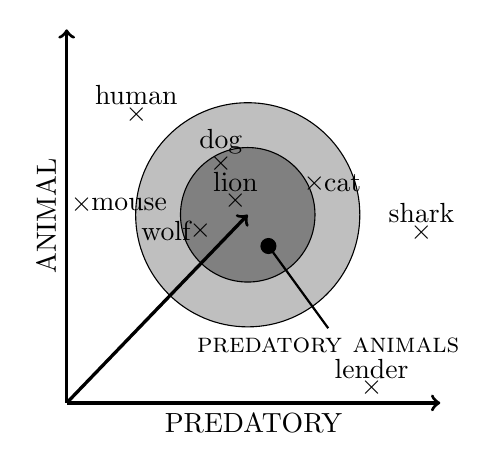
\begin{tikzpicture}
%    \begin{axis}[disabledatascaling,scale=1.75,axis equal,hide axis]
    \begin{axis}[disabledatascaling,scale=1,axis equal,hide axis]
%      \draw [fill = lightgray,fill opacity = 1.00] (3,3) circle [radius = 1.5];
%      \draw [fill = gray,fill opacity = 1.00] (3,3) circle [radius = 0.9];
      \draw [fill = lightgray,fill opacity = 1.00] (2.423,2.518) circle [radius = 1.5];
      \draw [fill = gray,fill opacity = 1.00] (2.423,2.518) circle [radius = 0.9];
      \node at (4.7477,2.2786) [above] {shark};
      \node at (4.7477,2.2786) {$\times$};
      \node at (2.0626,3.2008) [above] {dog};
      \node at (2.0626,3.2008) {$\times$};
      \node at (3.3145,2.9414) [right] {cat};
      \node at (3.3145,2.9414) {$\times$};
      \node at (4.0803,0.2) [above] {lender};
      \node at (4.0803,0.2) {$\times$};
      \node at (2.258,2.7022) [above] {lion};
      \node at (2.258,2.7022) {$\times$};
%      \draw [dotted] (3,3)--(2.258,2.7022) node [midway,above] {$a$};
      \node at (1.7883,2.3021) [left] {wolf};
      \node at (1.7883,2.3021) {$\times$};
      \node at (0.9311,3.8643) [above] {human};
      \node at (0.9311,3.8643) {$\times$};
%      \draw [dotted] (3,3)--(0.9311,3.8643) node [midway,above] {$b$};
      \node at (0.2,2.6516) [right] {mouse};
      \node at (0.2,2.6516) {$\times$};
      
      \addplot [->,very thick] coordinates{
      	(0,0)
        (2.423,2.518)
      };
      \node at (3.5,1.0) [below] {\textsc{predatory animals}};
      \addplot [thick] coordinates{
        (3.5,1.0)
        (2.7,2.1)
      };
      \draw [fill=black] (2.7,2.1) circle [radius = 0.1];
%      \addplot [->,dashed] coordinates{
%        (3,3)
%        (3.7,2.4343)
%      } node [midway,below] {$r_1$};
%      \addplot [->,dashed] coordinates{
%        (3,3)
%        (2.1,4.2)
%      } node [midway,above] {$r_2$};
      \addplot [->,very thick] coordinates{
        (0,0)
        (0,5)
      } node [midway,above,sloped] {ANIMAL};
      \addplot [->,very thick] coordinates{
        (0,0)
        (5,0)
      } node [midway,below] {PREDATORY};
    \end{axis}
  \end{tikzpicture}
  \caption{Word-vectors measured by proximity to a central point.}\label{fig:geo1-dist}
  \end{subfigure}
  \hspace*{0.05\textwidth}
  \begin{subfigure}[]{0.45\textwidth}
  \centering
  \small
  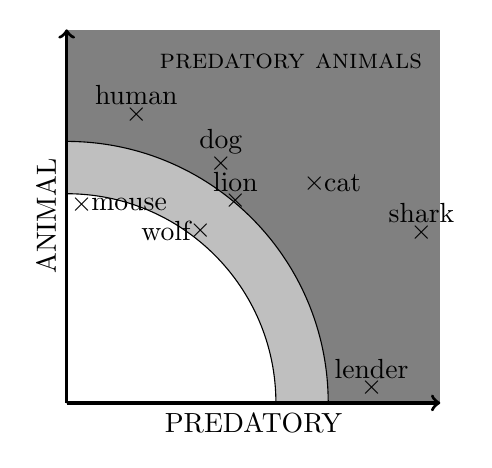
\begin{tikzpicture}
    \begin{axis}[disabledatascaling,scale=1,axis equal,hide axis]
      \draw [white,fill = gray,fill opacity = 1.00] (0,0) rectangle (5,5);
      \draw [fill = lightgray,fill opacity = 1.00] (0,0) -- (3.5,0) arc (0:90:3.5);
      \draw [fill = white,fill opacity = 1.00] (0,0) -- (2.8,0) arc (0:90:2.8);
      \node at (4.7477,2.2786) [above] {shark};
      \node at (4.7477,2.2786) {$\times$};
      \node at (2.0626,3.2008) [above] {dog};
      \node at (2.0626,3.2008) {$\times$};
      \node at (3.3145,2.9414) [right] {cat};
      \node at (3.3145,2.9414) {$\times$};
      \node at (4.0803,0.2) [above] {lender};
      \node at (4.0803,0.2) {$\times$};
      \node at (2.258,2.7022) [above] {lion};
      \node at (2.258,2.7022) {$\times$};
%      \draw [dotted] (0,0)--(2.258,2.7022) node [midway,above] {$a$};
      \node at (1.7883,2.3021) [left] {wolf};
      \node at (1.7883,2.3021) {$\times$};
      \node at (0.9311,3.8643) [above] {human};
      \node at (0.9311,3.8643) {$\times$};
%      \draw [dotted] (0,0)--(0.9311,3.8643) node [midway,above] {$b$};
      \node at (0.2,2.6516) [right] {mouse};
      \node at (0.2,2.6516) {$\times$};
      
      \node at (3,4.8) [below] {\textsc{predatory animals}};
%      \addplot [->,dashed] coordinates{
%        (0,0)
%        (2.8723,2.0)
%      } node [midway,below] {$r_1$};
%      \addplot [->,dashed] coordinates{
%        (0,0)
%        (2.6153,1.0)
%      } node [midway,above] {$r_2$};
      \addplot [->,very thick] coordinates{
        (0,0)
        (0,5)
      } node [midway,above,sloped] {ANIMAL};
      \addplot [->,very thick] coordinates{
        (0,0)
        (5,0)
      } node [midway,below] {PREDATORY};
    \end{axis}
  \end{tikzpicture}
  \caption{Word-vectors meansured in terms of distance from origin.}\label{fig:geo1-norm}
  \end{subfigure}
  \caption[Two Methods for Probing a Subspace]{Co-occurrence statistics for a small vocabulary construed along two hand-picked dimensions.  Darker regions are expected to be more conceptually prototypical for the context captured by these dimensions.}\label{fig:geo1}
\end{figure}

\subsection{Two Measures for Probing a Subspace} \label{sec:twomeasures}

In order to take a first pass at examining these robustly Euclidean features of my contextualised subspaces, I propose two geometric measures for exploring the conceptual geometry of a subspace, illustrated in Figure~\ref{fig:geo1}.  The first is a distance metric, which defines a central point in a subspace and then considers the relationship of words to the semantic context of the subspace in terms of the distance of the corresponding word-vectors from this central point.  The central point is defined as the mean point between the input word-vectors used to generate the subspace, or, for the purposes of Figure~\ref{fig:geo1-dist}, the central point of the eight word-vectors being analysed in this context.  In this subspace featuring two hand picked co-occurrence dimensions selected from a base model built from a 5x5 word co-occurrence window traversal of Wikipedia, word-vectors that for the sake of this example are relatively closely associated with the concept \textsc{predatory animal} turn up near this central point.\footnote{Here it happens to be the case that choosing dimensions which actually nominate a concept likewise delineate a space where, at least in terms of the restricted vocabulary evoked in Figure~\ref{fig:geo1}, conceptual membership plays out in a geometrically predictable way, but I will not generally presume this to be the case.}  So, for instance, \emph{cat} (certainly in the taxonomical sense of the denotation), more specifically \emph{lion}, then \emph{dog}, and, again more specifically, \emph{wolf} all fall close to the central point, while \emph{shark} (which certainly denotes a predator, and also an animal, but perhaps less prototypically so), \emph{mouse}, \emph{human}, and \emph{lender} are more distant.

The second measure deployed here will be to analyse the norms of the word-vectors projected into the contextualised subspace, with my hypothesis being that word-vectors that are relatively far from the origin will be correspondingly relevant to the conceptual context from which the subspace has been generated.  This prediction does not entirely play out in the subspace depicted in Figure~\ref{fig:geo1-norm}, where words like \emph{human} and \emph{lender} are about as far from the origin as \emph{cat} and \emph{shark}, and have larger norms than more prototypical denotations such as \emph{lion} and \emph{wolf}.  As will be seen in subsequent results, beginning here and extending into the experiments described in the next chapter, in higher dimensional subspaces selected using the techniques outlined above, norm does prove to be a predictive measure of semantic relevance.  Here again, the preponderance of co-occurrence statistics associated with a word over the course of a set of dimensions gives a higher dimensional subspace an advantage: if the selected dimensions are appropriately aligned, there will be a tendency for those word-vectors with some consistency of co-occurrence across all dimensions to extend towards the central fringe of the space, while those with inconsistent co-occurrence profiles will move towards the edges while remaining closer to the origin.

In the cases of both the distance from mean and norm measures, a threshold could, in principle, be established in order to determine a cut-off point for conceptual membership, either in terms of an absolute geometric measure -- a radius from either the central point or the origin -- or in terms of a set of nearest neighbours.  This step would begin to move these subspaces towards \citepos{Gardenfors2000} notion of a region within a conceptual space, particularly in the case of the distance based metric illustrated in Figure~\ref{fig:geo1-dist}: here a clear sense of convexity as a criterion for a conceptual region exists, and likewise of betweeness as an indicator of conceptual inclusion.  Importantly, though, these spaces as they stand lack the dimensional interpretability that characterises G\"{a}rdenfors's spaces, in that it is not possible to say that there is a dimension of size, or strength, or ferocity, or so forth along which a boundary for inclusion in the concept of \textsc{predatory animal} can be identified.

%\begin{table}
%\centering
%\small
%\begin{tabular}{ll|ll|ll|ll}
%\hline
%\multicolumn{4}{c}{\emph{lion, tiger, bear}} & \multicolumn{4}{|c}{\emph{dog, hamster, goldfish}} \\
%\multicolumn{2}{c}{\textsc{joint}} & \multicolumn{2}{c}{\textsc{indy}} & \multicolumn{2}{|c}{\textsc{joint}} & \multicolumn{2}{c}{\textsc{indy}} \\
%\hline
%norm & distance & norm & distance & norm & distance & norm & distance \\
%\hline
%leopard & cat & leopard & wild & hamsters & cat & dogs & cat \\
%langur & wild & dhole & cat & gerbils & pet & hamsters & giant \\
%hyena & wolf & hyena & giant & rabbits & monkey & sheepdog & animal \\
%dhole & elephant & rhinoceros & elephant & chinchillas & pig & terrier & wild \\
%boar & animals & leopards & lions & pet & rabbit & canine & animals \\
%tapir & giant & tapir & wolf & ferrets & rat & kennel & like \\
%macaque & animal & passant & animals & pigs & animal & akc & rabbit \\
%chital & bears & langur & tigers & rats & dogs & spaniel & include \\
%civet & dog & sumatran & cats & pets & giant & poodle & pig \\
%sloth & panther & gules & golden & chickens & cats & jerboa & cats \\
%\hline
%\end{tabular}
%\caption{The top word-vectors in spaces selected by input terms characteristic of \textsc{wild animals} and \textsc{pets}, for the \textsc{joint} and \textsc{indy} dimension selection techniques, measured in terms of top norms within each subspace and also word-vectors closest to the mean point between the input word-vectors.}
%\label{tab:tops}
%\end{table}

\begin{table}
\centering
\begin{tabular}{lll|lll}
\hline
\multicolumn{6}{c}{\emph{lion, tiger, bear}} \\
\multicolumn{3}{c}{\textsc{joint}} & \multicolumn{3}{c}{\textsc{indy}} \\
\hline
norm & distance & angle & norm & distance & angle \\
\hline
leopard & cat & and & leopard & wild & and \\
langur & wild & like & dhole & cat & as \\
hyena & wolf & also & hyena & giant & which \\
dhole & elephant & as & rhinoceros & elephant & like \\
boar & animals & such & leopards & lions & also \\
tapir & giant & well & tapir & wolf & be \\
macaque & animal & including & passant & animals & more \\
chital & bears & include & langur & tigers & including \\
civet & dog & from & sumatran & cats & been \\
sloth & panther & which & gules & golden & one \\
\hline
\end{tabular}
\caption[Top Wild Animal Word-Vectors]{The top word-vectors in subspaces selected by input terms characteristic of \textsc{wild animals}, for the \textsc{joint} and \textsc{indy} dimension selection techniques, measured in terms of top norms within each subspace (\emph{norm}), word-vectors closest to the mean point between the input word-vectors (\emph{distance}), and also the smallest angle with this mean vector regardless of actual position in the subspace (\emph{angle}).}
\label{tab:tops-wild}
\end{table}

Examples of the tendencies of both norms and relative distances are explored in Table~\ref{tab:tops-wild} and Table~\ref{tab:tops-pet}, where, as with the examples offered earlier in this chapter, input terms denoting things exemplary of the respective concepts \textsc{wild animals} and \textsc{pets} are used to generate subspaces, in this case using both the \textsc{joint} and \textsc{indy} dimension selection techniques, once again using a base space built using a 5x5 word co-occurrence window.  In these cases, the top 200 dimensions derived using each technique have been used to project subspaces, and then within those subspaces, the top ten word-vectors based on their norm and their distance from the mean point between the input word-vectors are reported.  In addition to the two geometric measures described above, as a point of comparison, I also present results using an angular measure, where the word-vectors with the highest cosine similarity with the vector of the mean point between the input word-vectors are returned.  This is offered as an approximation of what would be a typical approach in a standard static distributional model, to demonstrate why this measure doesn't work for the context sensitive spaces built using my methodology and also as a mechanism for further exploration of what's happening in these subspaces.

\begin{table}
\centering
\begin{tabular}{lll|lll}
\hline
\multicolumn{6}{c}{\emph{dog, hamster, goldfish}} \\
\multicolumn{3}{c}{\textsc{joint}} & \multicolumn{3}{c}{\textsc{indy}} \\
\hline
norm & distance & angle & norm & distance & angle \\
\hline
hamsters & cat & and & dogs & cat & also \\
gerbils & pet & also & hamsters & giant & as \\
rabbits & monkey & as & sheepdog & animal & in \\
chinchillas & pig & of & terrier & wild & which \\
pet & rabbit & in & canine & animals & and \\
ferrets & rat & such & kennel & like & like \\
pigs & animal & well & akc & rabbit & is \\
rats & dogs & - & spaniel & include & called \\
pets & giant & called & poodle & pig & of \\
chickens & cats & which & jerboa & cats & has \\
\hline
\end{tabular}
\caption[Top Pet Word-Vectors]{The top word-vectors in \textsc{joint} and \textsc{indy} subspaces, as in Table~\ref{tab:tops-wild} but selected by input terms characteristic of \textsc{pets}.}
\label{tab:tops-pet}
\end{table}

Notably, in the case of the norm measure, word-vectors that are exemplary of the conceptual category suggested by the intersection of the input terms seem to rise to the top of the subspace, so to speak: for both dimension selection techniques for the \textsc{wild animal} type inputs, a list of wild animals, some rather exotic, are returned.  A similar outcome is observed for the norm measure in the case of the \text{pet} inputs, with some admittedly disputable submissions such as \emph{rats} coming up in the \textsc{joint} output; jerboas, which are indicated in the \textsc{indy} output, are apparently a somewhat popular pet, and \emph{akc} presumably refers to the American Kennel Club, so, not a pet, but an institution related to pet keeping.  An interesting side effect of the \textsc{indy} technique in particular is that it returns a list including names of various dog breeds.  It would seem that the co-occurrence dimensions of the word-vectors for \emph{hamster} and \emph{goldfish} are characteristic enough of these more specialised words relating to particular types of pets that the corresponding word-vectors are pushed towards the fringe of the subspace.  It's also interesting that \emph{passant} and \emph{gules}, terms associated with the depiction of animals in heraldry, have high norms in the \textsc{indy} subspace for \textsc{wild animal} input in particular---of course all three of the input terms here are denotations of animals typical of heraldic devices, so it is not particularly surprising that some of their independently strong co-occurrence features combine to select for these word-vectors.

The distance measure returns roughly similar results, including a number of denotations of appropriate animals.  Here it is interesting to observe that other semantic types -- in particular, adjectives in addition to nouns -- begin to creep into the output: \emph{wild}, \emph{giant}, and \emph{golden} are returned in the \textsc{joint} and \textsc{indy} subspaces for the \textsc{wild animal} input, and \emph{giant} again comes up in response to the \textsc{pets} input, along with, perplexingly, the verb \emph{include}.  It makes sense that the region near the mean point between the input vectors, where consistently high but perhaps not absolutely maximal PMI scores across these contextually characteristic dimensions are to be found, feature some of the descriptors and predicates associated with the concept being modelled, while the region at the outer limit of the space, where the words with the highest overall PMI values across the dimensions of the subspace are to be found, seem to be pointed denotations of instances of the concepts in question.  The word-vectors corresponding to some of the more esoteric animals in particular are likely to have high co-occurrence frequencies with the dimensions selected by the combination of the input terms relative to low independent frequencies precisely because of their rareness.

Turning to the angular results, where words that are closest to the line extending through the mean point are returned, a sharp contrast to the other two geometric measures is observed.  Here, very generic words which serve as the structural components of language, contributing little in terms of specific meaning but crucial to the functional cohesion of utterances, are found in abundance.  This is completely logical: these types of words are liable to have a very consistent, albeit relatively low, profile of PMI scores across all dimensions in a subspace, since they are likely to have a high frequency of co-occurrences with any given word mitigated by correspondingly high independent frequencies across the corpus influencing the denominator of the PMI calculation.  The result is a word-vector populated by relatively low but also relatively uniform PMI values, situated not far from the origin and also very close to the centre line of the subspace.  This phenomenon highlights the discrepancy between the Euclidean, positively valued subspaces generated by my context sensitive methodology and the normalised, hyperspherical spaces built by conventional static distributional semantic models.  Because my subspaces have a sense of centre and periphery, as well as a sense of distance from the origin, it is possible to make both semantic and functional predictions about the types of words that will be found in different regions of a subspace, and accordingly to predict where to look -- and where not to look -- to discover geometries mapping to desired conceptual properties.

\subsection{Replete Geometric Analysis} \label{sec:replete}
I will now propose a general method for a replete geometric analysis of a contextually projected subspace, based on the position of word-vectors in a space as well as the relationship between those word-vectors and points based on a more general analysis of the dimensions delineating the subspace which I will characterise as \emph{generic points}.  For the purposes of explicating this method, I will presume a subspace projected from an analysis of two input word-vectors $A$ and $B$ using one of the dimension selection techniques described earlier in this chapter, a presumption in line with the experiments to be described in Chapters~\ref{chap:relsim} and~\ref{chap:figurative}.  The premise is that these word-vectors are to be analysed in terms of the semantic relationship between them; the precise nature of the relationship being analysed could be more or less anything, and in the next two chapters this method will be applied to the assessment of lexical similarity, relatedness, metaphor, and metonymy.  The objective of this analytic method will be first to test the hypothesis that the geometry of contextually projected subspaces should be semantically informative, and second to compare the aspects of the geometry that are most informative for different semantic phenomena.

\begin{figure}
\centering
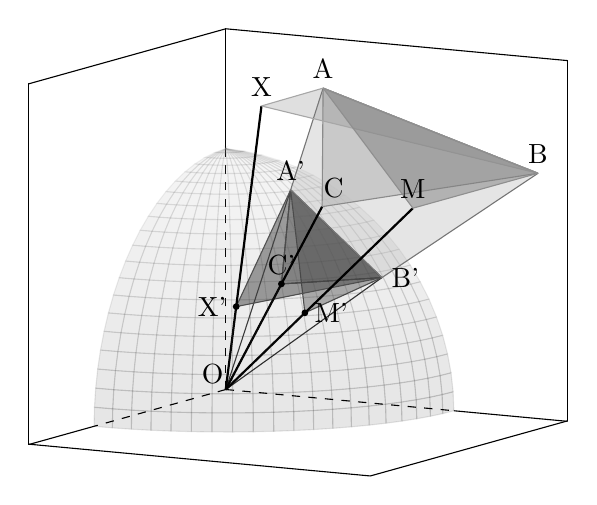
\begin{tikzpicture}
\begin{axis}[axis line style=white,view={120}{10},xmin=0,xmax=1.5,ymin=0,ymax=1.5,zmin=0,zmax=1.5,colormap/blackwhite,ticks=none]
\addplot3[color=black,thick] coordinates {(0,0,1.5) (0,1.5,1.5)};
\addplot3[color=black,thick] coordinates {(0,0,1.5) (1.5,0,1.5)};
\addplot3[color=black,thick] coordinates {(0,1.5,0) (0,1.5,1.5)};
\addplot3[color=black,thick] coordinates {(0,1.5,0) (1.5,1.5,0)};
\addplot3[color=black,thick] coordinates {(1.5,0,0) (1.5,0,1.5)};
\addplot3[color=black,thick] coordinates {(1.5,0,0) (1.5,1.5,0)};
\addplot3[color=black,dashed] coordinates {(0,0,0) (0,0,1)};
\addplot3[color=black,dashed] coordinates {(0,0,0) (0,1,0)};
\addplot3[color=black,dashed] coordinates {(0,0,0) (1,0,0)};
\addplot3[color=black] coordinates {(0,0,1) (0,0,1.5)};
\addplot3[color=black] coordinates {(0,1,0) (0,1.5,0)};
\addplot3[color=black] coordinates {(1,0,0) (1.5,0,0)};
\addplot3[patch,patch type=triangle,color=gray,fill opacity=0.0] coordinates {(0.0,0.0,0.0) (0.5774,0.5774,0.5774) (0.2,0.4,0.8944)
};
\addplot3[patch,patch type=triangle,color=gray,fill opacity=0.0] coordinates {(0.0,0.0,0.0) (0.5774,0.5774,0.5774) (0.2,0.8,0.5657)
};
\addplot3[patch,patch type=triangle,color=darkgray,fill opacity=0.25] coordinates {(0.5774,0.5774,0.5774) (0.2,0.4,0.8944) (0.2,0.8,0.5657)
};
\addplot3[patch,patch type=triangle,color=darkgray,fill opacity=0.4] coordinates {(0.5709,0.6766,0.4651) (0.2,0.4,0.8944) (0.2,0.8,0.5657)
};
\addplot3[patch,patch type=triangle,color=darkgray,fill opacity=0.5] coordinates {(0.7309,0.4678,0.4970) (0.2,0.4,0.8944) (0.2,0.8,0.5657)
};
\addplot3 [color=black,thick] coordinates {(0,0,0) (0.5774,0.5774,0.5774)};
\addplot3 [color=black,thick] coordinates {(0,0,0) (0.7309,0.4678,0.4970)};
\addplot3 [color=black,thick] coordinates {(0,0,0) (0.5709,0.6766,0.4651)};
\addplot3[opacity = 0.1,surf,z buffer = sort,samples = 21,variable = \u,variable y = \v,domain = 0:90,y domain = 0:90,]
    ({1*cos(u)*sin(v)}, {1*sin(u)*sin(v)}, {1*cos(v)});
\addplot3 [patch,patch type=rectangle,color=lightgray,fill opacity=0.4] coordinates{(0.2,0.4,0.8944) (0.3,0.6,1.35) (0.4,1.6,1.1) (0.2,0.8,0.5657)};
\addplot3 [color=black,thick] coordinates {(0.5774,0.5774,0.5774) (1.0,1.0,1.0)};
\addplot3 [color=black,thick] coordinates {(0.7309,0.4678,0.4970) (2.5,1.6,1.7)};
\addplot3 [color=black,thick] coordinates {(0.5709,0.6766,0.4651) (1.35,1.6,1.1)};
\addplot3 [patch,patch type=triangle,color=lightgray,fill opacity=0.75] coordinates{(0.3,0.6,1.35) (1.0,1.0,1.0) (0.4,1.6,1.1)};
\addplot3 [patch,patch type=triangle,color=gray,fill opacity=0.25] coordinates{(0.3,0.6,1.35) (2.5,1.6,1.7) (0.4,1.6,1.1)};
\addplot3 [patch,patch type=triangle,color=gray,fill opacity=0.5] coordinates{(0.3,0.6,1.35) (1.35,1.6,1.1) (0.4,1.6,1.1)};
\node [anchor=south] at (axis cs: 0.1,0.0,0.0) {O};
\node [anchor=south] at (axis cs: 0.3,0.6,1.35) {A};
\node [anchor=south] at (axis cs: 0.4,1.6,1.1) {B};
\node [anchor=south] at (axis cs: 0.2,0.4,0.8944) {A'};
\node [anchor=west] at (axis cs: 0.2,0.8,0.5657) {B'};
\node [anchor=south] at (axis cs: 0.5774,0.5774,0.5774) {C'};
\draw plot [mark=*, mark size=1] coordinates{(axis cs: 0.5774,0.5774,0.5774)};
\node [anchor=south] at (axis cs: 1.0,1.05,1.0) {C};
\node [anchor=east] at (axis cs: 0.7309,0.4678,0.4970) {X'};
\draw plot [mark=*, mark size=1] coordinates{(axis cs: 0.7309,0.4678,0.4970)};
\node [anchor=south] at (axis cs: 2.5,1.6,1.7) {X};
\node [anchor=west] at (axis cs: 0.5709,0.6766,0.4651) {M'};
\draw plot [mark=*, mark size=1] coordinates{(axis cs: 0.5709,0.6766,0.4651)};
\node [anchor=south] at (axis cs: 1.35,1.6,1.1) {M};
\end{axis}
\end{tikzpicture}
\caption[Geometric Features of Contextualised Subspaces]{The geometric features of a subspace contextually projected based on an analysis of two input word-vectors.}
\label{fig:geofull}
\end{figure}

Figure~\ref{fig:geofull} illustrates a generic three dimensional subspace, with point $O$ as the origin.  Points $A$ and $B$ are the two word-vectors that have been used to select the dimensions which define this subspace, and are likewise the word-vectors which will be analysed through the geometry of the subspace.  In addition to these two vectors explicitly defined in terms of the values of projected word-vectors, two points are established based on an overall analysis of the dimensionality of the subspace: the \emph{mean vector} $M$ and the \emph{maximal vector} $X$.  $M$ is defined as the vector of all the mean values for all the dimensions $J$ delineating the subspace, so, if the dimensionality of $J$ is $d$, M can be defined formally as follows:

\begin{equation}
M := \{\mu(J_{1}),\ \mu(J_{2})...\ \mu(J_{d})\}
\end{equation}

\noindent And likewise, $X$ can be expressed in terms of an equation:

\begin{equation}
X := \{max(J_{1}),\ max(J_{2})...\ max(J_{d})\}
\end{equation}

\noindent Finally, a generic central vector $C$, with all dimensions set to the same value, is defined.  The universal value chosen to define the dimensions of this vector is the mean value of the mean vector $M$, so, formally, this point is the vector of that mean value repeated $d$ times:

\begin{equation}
C := \{\mu(M)_1,\ \mu(M)_2... \mu(M)_d\}
\end{equation}

\noindent In the analysis of the semantic relationship between $A$ and $B$ in a given projection, these three vectors will be used as anchor points to establish the situation of $A$ and $B$ relative to the subspace overall: where $C$ is an objectively central point in the subspace, $M$ is in a sense central to a subspace relative to its particular dimensional constitution, and $X$ is similarly indicative of the outermost possible extent of a particular subspace.  The underlying intuition here is that, due to the frequentist components of the information theoretic co-occurrence statistics used to build the base space, different dimensions have different distributional profiles.  To demonstrate this point, Table~\ref{tab:profiles} presents the mean values and standard deviations for the distribution of mean and maximum points from the top 20,000\footnote{Less frequent dimensions tend to have higher PMI values overall, and also tend to be products of co-occurrences observed in quite obscure passages of the base corpus---it's worth recalling that a little more than half of the co-occurrence dimensions are observed only once.} most frequent co-occurrence dimensions, as well as the top five and bottom five values for each of these statistics for illustrative purposes.

\begin{table}
\centering
\begin{tabular}{lr|r}
\hline
& \multicolumn{1}{c}{\textsc{mean}} & \multicolumn{1}{c}{\textsc{max}} \\
\hline
\parbox[t]{2mm}{\multirow{5}{*}{\rotatebox[origin=c]{90}{\textsc{top}}}} & \emph{sofla:} 6.984 & \emph{nico:} 15.690 \\
& \emph{olya:} 6.326 & \emph{yeah:} 15.610 \\
& \emph{non-families:} 6.035 & \emph{superfamily:} 15.598 \\
& \emph{gmina:} 5.364 & \emph{eel:} 15.483 \\
& \emph{crambidae:} 5.485 & \emph{kermanshah:} 15.455 \\
\hline
\parbox[t]{2mm}{\multirow{5}{*}{\rotatebox[origin=c]{90}{\textsc{bottom}}}} & \emph{it:} 0.748 & \emph{he:} 3.903 \\
& \emph{they:} 0.812 & \emph{in:} 3.449 \\
& \emph{you:} 0.804 & \emph{of:} 3.379 \\
& \emph{this:} 0.789 & \emph{to:} 3.120 \\
& \emph{he:} 0.719 & \emph{and:} 2.993 \\
\hline
mean & 2.312 & 11.066 \\
std & 0.396 & 1.607 \\
\hline
\end{tabular}
\caption[Mean and Maximum PMI Values]{Dimensional profiles in terms of mean and maximum PMI values along dimensions, including mean values and standard deviation as well as the top five and bottom five dimensions for each statistic.}
\label{tab:profiles}
\end{table}

The co-occurrence dimensions that tend to have lower mean and maximum values are clearly quite frequent words, and this is to be expected, given that the high frequency of independent observations of the word will drive PMI scores down for that word across the board.  The emergence of relatively infrequent words at the top end of the spectrum is then also to be expected.\footnote{The appearance of \emph{yeah} as one of the dimensions with a particular high maximum value is interesting, and perhaps surprising, though it should be noted that this is a particularly un-Wikipedian word, and is likely to occur in the context of things like quotations and band names, where co-occurrence with likewise obscure terms is more likely.}  The main point to note here, though, is that there is a broad range of possible mean and maximum values for a given dimension, and so the vectors $M$ and $X$ might be expected to vary considerably from subspace to subspace.  Moreover, this variance may in turn correspond to semantic features of a given subspace: it may be the case that a given type of relationship between input terms -- terms which are similar or dissimilar, literal or figurative in relationship to one another -- select for a subspace which has a particular orientation in terms of its dimensional profile.  A final observation here regards the way that the distribution of mean and maximum dimensional values skew, with means tending to clump towards the low end of the spectrum while maximums are more dense at the high end of the spectrum.  More specific conjectures and results will be presented throughout the next two chapters.

In addition to the situation of the vectors $A$, $B$, $C$, $M$, and $X$ in a subspace, a normalised version of the subspace is considered, in which each vector is effectively measured at its intersection with a hypersphere of radius 1 emanating from the origin.  These points are represented as $A'$, $B'$, $C'$, $M'$, and $X'$ respectively in Figure~\ref{fig:geofull}.  The purpose of considering these points is to take measure of the way in which the various vectors in a given subspace relate to the subspace as a whole, regardless of the extent of these vectors.  So, for instance, the vectors $A$ and $B$ might have very different norms, but the distances between $A'$, $B'$, $C'$, $M'$, and $X'$ might still be very small---and, even then, the angle $\angle A'M'B'$ might be very large, suggesting that $A$ and $B$ both pass through the central region of the subspace but on different sides of the generic central point of the subspace.  One of the objectives of this analytical method is to test whether this kind of information, which can be captured through a robust geometric description of a subspace, is semantically indicative.

So finally the various geometric features available for the analysis of a subspace are systematically outlined in Table~\ref{tab:features}.  The points to be found in the space are broken down into three types, namely, the word-vectors themselves (points $A$ and $B$), the generic vectors that emerge from an analysis of a subspace (points $C$, $M$, and $X$), and the normalised versions of all these points ($A'$, $B'$, $C'$ $M'$, and $X'$).  The relationships between these vectors are construed across five categories as follows:

\begin{description}
\item[Distances] Euclidean distances, such as the distance between the two word-vectors $A$ and $B$ as well as the norms of the generic points, and, additionally, the mean distance of $A$ and $B$ from the origin;
\item[Angles] The angles at the vertexes of the generic points of a subspace, so for instance $\angle ACB$ formed by lines $\overline{AC}$ and $\overline{BC}$, as well as the normalised versions of these angles, and also the angles formed between the vectors of the generic points such as $\angle COM$;
\item[Means] The average norms of the word-vectors and the average distances from the word-vectors to generic points as well as the average distances of the normalised versions of these points;
\item[Ratios] The ratio of the norms of the word-vectors and of the distances from the word-vectors to generic points, taking the lower of the two distances as the denominator, as well as the normalised version of the same measures;
\item [Fractions] The ratio of the mean distance from the origin of $A$ and $B$ to each of the three generic points, as well as the ratios of the generic points to one another.
\end{description}

\begin{table}
\centering
\begin{tabular}{ll}
\hline
\multicolumn{2}{c}{\textsc{distances}} \\
word-vectors & $\overline{AB}$ \\
generic points & $C$, \quad $M$, \quad $X$ \\
\hline
\multicolumn{2}{c}{\textsc{angles}} \\
word-vectors & $\angle AOB$, \quad $\angle ACB$, \quad $\angle AMB$, \quad $\angle AXB$ \\
normalised & $\angle A'C'B'$, \quad $\angle A'M'B'$, \quad $\angle A'X'B'$ \\
generic points & $\angle COM$, \quad $\angle COX$, \quad $\angle MOX$ \\
\hline
\multicolumn{2}{c}{\textsc{means}} \\
word-vectors & $\mu (A,B)$, \quad $\mu (\overline{AC},\overline{BC})$, \quad $\mu (\overline{AM},\overline{BM})$, \quad $\mu (\overline{AX},\overline{BX})$ \\
normalised & $\mu (\overline{A'C'},\overline{B'C'})$, \quad $\mu (\overline{A'M'},\overline{B'M'})$, \quad $\mu (\overline{A'X'},\overline{B'X'})$ \\
\hline
\multicolumn{2}{c}{\textsc{ratios}} \\
word-vectors & $A:B$, \quad $\overline{AC}:\overline{BC}$, \quad $\overline{AM}:\overline{BM}$, \quad $\overline{AX}:\overline{BX}$ \\
normalised & $\overline{A'C'}:\overline{B'C'}$, \quad $\overline{A'M'}:\overline{B'M'}$, \quad $\overline{A'X'}:\overline{B'X'}$ \\
\hline
\multicolumn{2}{c}{\textsc{fractions}} \\
word-vectors & $\mu (A,B)/C$, \quad $\mu (A,B)/M$, \quad $\mu (A,B)/X$ \\
generic points & $C/M$, \quad $C/X$, \quad $M/X$ \\
\hline
\end{tabular}
\caption[Schematic of Geometric Features]{Geometric features extrapolated from a subspace projected based on an analysis of two two input terms $A$ and $B$.}
\label{tab:features}
\end{table}

\noindent These features have been selected as indicative of the overall comportment of the subspaces from which they are extracted, and, both independently and in conjunction, are expected to serve as indicators of the semantic phenomena characteristic of the word-vectors used to generate the subspace into which they are projected.  So, for instance, I will predict (incorrectly, it turns out) that the distance $\overline{AB}$ will be one of the strongest indicators of semantic relatedness.  Furthermore, the extrapolation of the generic features of a subspace is expected to indicate more general patterns of co-occurrence that are associated with semantic phenomena such as similarity and metaphor.  When dimensions with similar mean value are jointly selected by a pair of words, a (more correct) expectation will be that this indicates a high degree of conceptual overlap between the words' referents, and therefore a high degree of similarity.

As a more general hypothesis, I surmise that different sets of geometric features will collectively be predictive of different semantic phenomena.  One of the primary objectives of the empirical work described in the next two chapters will be to establish a methodology for mapping features to phenomena and then using these correspondences as a mechanism for understanding the statistical characteristics that allow for the computational extraction of semantically and contextually useful information from large scale corpora.  It will therefore ultimately be the comparison of the groupings of features corresponding to specific semantic phenomena that will provide the most significant outputs of the research reported here, and so the arrangement of features in terms of types and categories as outlined in Table~\ref{tab:features} is in this regard a schematic for the computational experimentation and corresponding evaluation and analysis at the core of this thesis.

The intuition behind the selection of the generic vectors outlined above is that they will provide a kind of pivot for gauging the situation of word-vectors both in relation to the defining features of the subspace the occupy as well as to one another relative to these features.  So the relationship between a word-vector $A$ and the generic vector $C$ and $M$ will give two different perspectives on the centrality, so to speak, of $A$.  At the same time, the relative relationship between word-vectors $A$ and $B$ in comparison to, say, $M$, as measured by $\angle AMC$, will offer a sense of whether the word-vectors are on the same or different side of the centre of the space, and so will offer a very broad sense of regionalism and perhaps corresponding conceptual categorisation developing within a subspace.  The features outlined in Table~\ref{tab:features} are designed to present a ready-made overview of the potential conceptual geometry of any given subspace.

\section{A Mathematical Justification for Geometric Analysis} \label{sec:math}
The application of geometry as a productive analytical tool for extrapolating semantic information from contextualised co-occurrence statistics has been, thus far, presented as a somewhat intuitive decision.  There is a certain elegance to using quantifiable distances and angles as the analytical representation of choice, and this approach will, it will be seen, assist in the visualisation of what's happening statistically in the subspaces produced by my model.  Notwithstanding these benefits, this section will offer a more mathematically thorough explanation of why a geometric approach is the right one for the types of statistics that are being used here, and in probabilistic models in general.

In order to understand the usefulness of geometry, it is worthwhile to consider again the information theoretical nature of the statistics being used here, and more generally in a plethora of distributional semantic models.  Specifically, revisiting and restating Equation~\ref{eq:MI}, the scalars of the base model are defined by considering a ratio of frequencies approximately equivalent to a ratio of probabilities (and this equation is approximate because we are ignoring the constants defined in Section~\ref{sec:pmi}):

\begin{equation}
PMI(w,c) \approx \log\left(\frac{p(w,c)}{p(w) \times p(c)}\right)
\end{equation}

\noindent In other words, PMI values are logarithms of probabilities, and logarithms have the natural property of translating products and ratios into sums and differences.  So, for instance, if we have an operation such as $PMI(w_1,c)-PMI(w_2,c)$, we can express this as a log of a ratio of products of probabilities:

\begin{equation}
PMI(w_1,c)-PMI(w_2,c) \approx \log\left(\frac{p(w_1,c) \times p(w_2) \times p(c)}{p(w_2,c) \times p(w_1) \times p(c)} \right)
\end{equation}

\noindent This, in turn, actually just reduces to a ratio of conditional probabilities:

\begin{equation} \label{eq:logdif}
PMI(w_1,c)-PMI(w_2,c) \approx \log\left(\frac{p(c|w_1)}{p(c|w_2)}\right)
\end{equation}

\noindent Next it must be noted that the geometry of the features described in Table~\ref{tab:features} are in large part derived from the vectors between the various points of interest -- word-vectors as well as generic features -- in a contextualised subspace.  These vectors can now be understood as concatenations of logarithms of ratios of the pointwise conditional probabilities of the dimensions delineating a $d$ dimensional context:

\begin{equation}
\overrightarrow{w_1}-\overrightarrow{w_2} \approx \left\{ \log\left(\frac{p(c_1|w_1)}{p(c_1|w_2}\right), \log\left(\frac{p(c_2|w_1)}{p(c_2|w_2)}\right)... \log\left(\frac{p(c_d|w_1)}{p(c_d|w_2)}\right)\right\}
\end{equation}

\noindent So from this perspective, the various features used to analyse the semantic situation of lexical representations in a contextualised subspace are, in fact, operations on conditional probabilities derived from observations of co-occurrence dimensions in the vicinity of target words.  This then becomes a recapitulation of my hypothesis, namely, that there should be a mechanism for exploring how the semantic context in which word meaning comes about can be captured in terms of a way of talking about things, with this way of talking mapping more specifically to a set of conditional probabilities relating to the chances of finding a particular context term in the vicinity of a target word (or, indeed, the average or maximal probability of finding that context term, as with the generic vectors of a subspace).  The dimensional selection techniques proposed earlier in this chapter are now effectively three postulates about methods for discovering the set of co-occurrence terms which should be considered in the context of the conditions of target word-vectors and generic vectors in a subspace.

Furthermore, when we consider the various geometric features of a contextualised subspace as the independent variables of a model designed to classify or quantify a semantic phenomenon, we are in fact looking for weighted linear combinations of operations on conditional probabilities that maximise the correlation between those statistics and a set of dependent variables generally based on human observations.  In Chapter~\ref{chap:relsim}, for instance, a linear regression will be used to try to learn to predict human ratings of relatedness and similarity based on geometric features of subspaces, and in Chapter~\ref{chap:figurative} a logistic regression will be used to similarly classify binary judgements of metaphoricity.  At this point, the geometry of the subspaces generated by my methodology becomes not only a convenient mechanism for humans to use to visualise the relationships between various statistical spaces, but actually also a handle for an algorithm to selectively learn rather complex combinations of probabilistic features.  A machine learning approach to analysing the geometry of a contextualised subspace then becomes a mechanism for iterating through inferential expressions formulated as operations on conditional probabilities, and an effective model will extrapolate an interpretable treatment of these probabilities directly from the geometry of a subspace.

\section{Comparing to Alternative Approaches}
In order to evaluate the effectiveness of my methodology, it will naturally be necessary to compare the performance of the models I develop against other models.  One way of doing this will, of course, be to compare to results other researchers have obtained experimenting with the data which will serve as the foundation for the results reported in the next three chapters.  In the cases of results reported by other researchers, though, similar but variously different corpora have been used to train other models described in the literature.  This is to be expected, and the results for large scale corpora should be fairly generalisable assuming a sensible choice of data (and the use of Wikipedia as all or a large portion of base data is quite common in the field), but nonetheless it will be useful to establish a baseline of results generated using models trained on the exact corpus to which I apply my methodology.  And in the cases of metaphor and semantic type coercion in particular, which will be examined in Chapter~\ref{chap:figurative}, the datasets explored are relatively new and have not been approached by many researchers in the field, so any additional point of comparison will be valuable in evaluating my methodology.

Moreover, in most cases, other models have been designed in a task specific way: so, for instance, \cite{SchwartzEA2015} have developed a syntactic heuristic for identifying semantic similarity as compared to relatedness in particular, and \cite{GutierrezEA2016} describe a model that generates compositional adjective-noun representations geared towards metaphor detection.  One of the key features of my models is that they are intended to be \emph{general}: the geometries generated by my methodology are expected to be replete with semantic interpretability, allowing for the same potential for diverse and often surprising conceptualisation corresponding to the infinitely combinatory characteristic of natural language in use.  For this reason, it is desirable to have a base case of a static model that can be compared across the board to all the different tasks handled by my methodology.

With all this in mind, I propose two different points of comparison that, in addition to results extracted from existing literature, will be applicable to all subsequent experiments described here.  The first involves factorising my base space using singular value decomposition (SVD), abstracting the space into a smaller set of abstract dimensions representing axes of maximum variance between PMI values.  The second is an application of a well known and highly productive neural network model to the same underlying data that I've used.  This will serve as a mechanism for comparing my results to what has proved to be another very effective methodology for the statistical modelling of semantics in general.

\subsection{Static Interpretations of the Base Space}
Using the dimension reduction techniques described by, for instance, \cite{DeerwesterEA1990} in the context of latent semantic analysis, it is possible to directly transform the same base spaces used for my context sensitive projections into a static model consisting of word-vectors defined along dimensions abstracted away from co-occurrence statistics in order to instead represent maximal axes of variance across the underlying data.  The mathematical technique applied here is a low rank approximation of a singular value decomposition of the full blown co-occurrence matrix.  To revisit this linear algebraic procedure, a $c \times d$ co-occurrence matrix $M$ can be decomposed into three separate matrices, two orthonormal matrices $U$ of shape $c \times r$ and $V$ of shape $d \times r$ and a diagonal $r \times r$ matrix $\sigma$ of eigenvalues, where $r$ is the rank of $M$, such that $M$ is the product of the decomposition:

\begin{equation}
M = U \Sigma V^{T}
\end{equation}

\noindent In order to find an approximation of the variance between word vectors, a $k$ dimensional matrix $U\hat{\Sigma}U'$ can be derived by setting all but the top $k$ values in $\Sigma$ to zero in $\hat{\Sigma}$.  Since the highest eigenvalues in $\Sigma$ will correspond to the orthonormal decomposition of dimensions with the highest variance between word-vectors, the resulting lower dimensional matrix will contain maximal information about interrelationships between word-vectors.  Some authors, including \citeauthor{DeerwesterEA1990} and, more recently, \cite{TurneyEA2010} have argued that the dimensions of such an approximation can be understood to correspond to conceptual axes across the data.

Of course, as mentioned in Chapter~\ref{sec:litdims}, the matrices derived through such a process of factorisation and recomposition effectively abstract away from any interpretability in terms of their dimensions, which now just represent orthogonal axes of maximal variance, and so they are insusceptible to my methodology for contextual dimensional reduction.  My case is that, when it comes to deriving spaces where the conceptual underpinnings of semantics play out in terms of geometric relationships between lexical representations, the geometries necessarily must be supplied in a context specific, online manner.  Gauging the difference in performance between the SVD decomposition of my base spaces and the contextualised subspaces generated using the dimension selection techniques described above will provide a basis for comparing the extent to which each approach really does manage to extract conceptually significant relationships from the underlying co-occurrence data.

Because my base spaces are sparse and positive, the dense matrix resulting from the operation of an SVD approximation is skewed from the centre of the resulting lower dimensional space.  To compensate for this, I take a final step in order to facilitate the calculation of semantic relationships between words in terms of the angular situations of the corresponding word-vectors: I translate and then scale the matrix by performing mean zero, standard deviation one normalisation across all dimensions of the reduced matrix.  This means the reduced space resembles something very much like the hyperspheres derived from the neural network approach to distributional semantics which will be described in the next section, and, as will be seen in the experiments carried out over the next three chapters, it has an interesting impact on model output.

%In cases where the geometry being explored involves just target word-vectors and generic points of a space -- so, for all the features described in Table~\ref{tab:features} -- it is computationally tractable to treat the sparse base matrix from which subspaces are projected as a semantically interpretable space in its own right.  This is because universal generic points (the mean point for all dimensions, the maximum point for all dimensions, and the central point based on the average value of the mean point) can be discovered through a one-off calculation, and the word-vectors themselves will be relatively sparse.  In the most onerous case of comparing two orthogonal word-vectors using the \textsc{indy} technique, the total number of scalars involved in the computations of geometric features would be the sum of the number of non-zero dimensions for each word-vector, so something on the order of thousands to tens of thousands of values---not that bad, computationally speaking.

%Of course, the norms of the generic points in such a general space will be extremely high compared to any given actual word-vector, since these generic points will have non-zero values in several million dimensions.  With this in mind, a second and more typical approach to building a general and computable distributional semantic space out of my base space of co-occurrence statistics is to through matrix factorisation: using singular value decomposition, I project the base space onto the top most informational eigenvectors up to a dimensionality to match the parameters tested using my context specific dimensional selection techniques.\footnote{In practice, the \texttt{sklearn} python module's PCA method is used to do this.}  Because of computability constraints, I take the top 100 to 50,000 most frequent word types as the vocabulary for this model, and consider the top 10,000 most frequent co-occurrence terms as the dimensions of the matrix to be factorised.  This means that 1,979 of the 1,998 word tokens in the SimLex999 dataset \citep[][discussed in detail in Chapter~\ref{chap:concepts}]{HillEA2014} are included in the vocabulary, and almost 90\% of the co-occurrence observations tabulated in the base space are represented in the decomposed model.

%Because SVD produces a space in which dimensions are characterised by variance rather than extent (meaning that signs can be reversed along a given dimension, and the barycentre is typically at the origin), the factorised model is not suitable for generating the generic points which are key features of my contextual models.  In order to make the most fair comparisons possible, this factorised model will be shifted in the case of each analysis of a set of word-vectors $W$ such that those word-vectors have the highest possible value along a dimension $D$ in the set of top eigenvectors, with the value furtherest from the mean of the word-vectors being reset to zero:

%\begin{equation}
%d_i' = |d_i-\argmax_{d \in D}(\mu\{d_w:w \in W\}-d)|
%\end{equation}

%This shifting procedure in practice introduces a degree of context to the generic dimension reduction technique, allowing for new geometric relationships between word-vectors and emergent generic points of the model to be established for each set of inputs; the distances between the word-vectors themselves, meanwhile, are unaffected.  In the end this will simply re-enforce the point that the difficulty of systematically applying context using more typical dimension reduction techniques is one of the strengths of my methodology.

\subsection{A Model Trained Using a Neural Network} \label{sec:w2v}
In addition to the interpretations of the statistical base space described above, the neural network based models outlined by \cite{MikolovEA2013b} under the rubric \texttt{word2vec} will be used as a point of comparison.  These models have received a remarkable degree of attention in the NLP literature since their introduction a few years ago, so much so that the software was mentioned by name in 116 out of the 230 long papers published in the 2016 Proceedings of the Meeting for the Association for Computational Linguistics \citep{ErkEA2016}.  The models have been taken, sometimes in modified form, as a source for representations of words \emph{embedded} in vector spaces trained on large scale textual data, applied to tasks ranging from word relatedness and similarity ratings \citep{KielaEA2015} to analogy completion \citep{MikolovEA2013}, and have also been applied to multimodal tasks such as image labelling \citep{KotturEA2016}.

The \texttt{word2vec} framework includes two different neural network architectures for generating word-vector representations based on traversals of large scale corpora.  The \emph{contextual bag of words} (CBOW) technique treats the terms in a co-occurrence window surrounding a target word $w$ as input and attempts to learn a representative word-vector $\overrightarrow{w}$ that is predicted by processing the input word-vectors through a recursive neural network.  The \emph{skip-gram} technique, on the other hand, treats the representation $\overrightarrow{w}$ itself as input to a network which learns to predict word-vectors representing words on either side of the target word.  In both cases, the model updates the scalars of the target word vectors in order to move them closer to the vectors representing each co-occurrence in which they're observed through backpropagation.  In the case of the CBOW model, the terms co-occurring within a given window of the target word are combined into an average vector for the purpose of each training observation; with the skip-gram model, the selection of target output word-vectors is weighted based on their distance from the input word-vectors, and the model optimises the probability of two word vectors interpreted via the softmax function \citep[see][for more details]{MikolovEA2013c}.

In addition to the size of the co-occurrence window, model parameters include the number of iterations of the corpus, the architecture of the single-layer network connecting input to output vectors, and, in the case of the skip-gram model, a rate of negative sampling by which random sets of words are taken as instances of non-co-occurrences and used to push the corresponding word-vectors away from the input word-vector.  The skip-gram model, with its sensitivity to word order, has been reported to perform particularly well on analogy completion task involving semantic similarity, so for instance in discovering the relationship \emph{king:queen::man:woman}.  The CBOW model, on the other hand, has performed better on what the authors have described as \emph{syntactic} analogies such as \emph{good:better::bad:worse}.

Here, the skip-gram and CBOW techniques of \texttt{word2vec} will be taken as exemplars of general-purpose distributional semantic modelling.  For the purposes of a fair comparison, I've trained instances of both models using the same cleaned corpus described in the previous chapter and used to train my own model.  The presumption, corroborated by the wide applications found for the models and described by various authors over the past three years, is that this approach provides a general framework for generating a space in which word-vectors relate to one another in conceptually productive ways.  A primary difference between the vectors learned by \texttt{word2vec} and the vectors representing word co-occurrence statistics derived by my model is that \texttt{word2vec} produces dense vectors whose dimensions cannot be individually interpreted as corresponding to any specific set of observations across a corpus, whereas my model generates a base space of sparse vectors for which each dimension maintains its status as an indication about a tendency of co-occurrences with a specific term.  This dimensional interpretability gives my model its power of contextualisation.

Following from this, it should also be noted that in the \texttt{word2vec} models, as is likewise typically the case with models generated using principle component analysis, semantic relationships are measured in terms of cosine similarity between word-vectors, which means that the models are treated as effectively normalised vector spaces centered at the origin.  A consequence of this normalisation and centering is that these spaces lack a sense of perimeter and extent, which means that they can't be interpreted in terms of the relationship between word-vectors and generic points characteristic of a contextual subspace, as described above.  These two features of my methodology, its ability to generate subspaces contextually and its capacity for nuanced geometric interpreation, are the two essential points that will be examined in the experiments described in the next two chapters.

\section{A Proof of Concept}\label{sec:poc}
In this section, I present a preliminary experiment performed using my contextually dynamic distributional semantic model.  This experiment, conceived as a proof of concept, involves using multi-word phrases as input and evaluating my methodology's capacity for building subspaces where words associated with the conceptual category denoted by the input term can be reliably discovered.  The experiment expands upon the notion of proto-conceptual spaces outlined in Section~\ref{sec:twomeasures}, examining whether the word-vectors that populate regions of subspaces are characterised by a certain categorical coherence.  In the case of the data explored here, the experiment is specifically set up to feel out the contextual capacity of my methodology and compare it to a standard generic semantic space.  The question asked is whether the shifts from subspace to subspace based on particular input yield productive alterations in the way that words both cluster and emerge from the melange of word-vectors that circulate around my base model.

The gist of this experiment is to take a word pair representing a compound noun -- for instance, \emph{body part} -- and see if my methodology can use the word pair to contextually generate a space where other words conceptually related to that compound noun can be found in a systematic way.  This is conceived of as an entailment task, in that I will attempt to find phrases considered to be categorical constituents of the concept represented by the word pair, taking the WordNet lexical taxonomy as a ground truth.  There is a scholastic back story here.

An early version of this experiment was reported in \cite{AgresEA2015}.  That first effort arose out of a question posed by a colleague regarding the feasibility of using a statical NLP technique for generating categorical labels that could be used to evaluate computational creativity in a domain specific way \citep[for a psychological perspective on the difficulty of generating such terms in an objective way using human subjects, see][]{VanDerVeldeEA2015}.  So, for instance, given a creative domain such as \textsc{musical creativity}, could a distributional semantic model generate terms that are reliably relevant to the concept denoted by that phrase, rather than the potentially disparate properties independently associated with \textsc{music} and \textsc{creativity}?  Intuitively there seems to be little reason to hope that the space halfway between these points in a general semantic space would somehow adequately represent the properties of the overall concept.  The early work explored the dimensions contextually selected by analysing the co-occurrence features of word-vectors corresponding to inputs along the lines of the expository results presented anecdotally in Chapter~\ref{chap:method}, but without any rigorous evaluation.

Reviewer responses to a subsequent journal article \citep{McGregorEA2015c}, designed as a more thorough introduction of the methodology, inspired a computationally oriented mode of evaluation.  The experiment that has emerged involves attempting to recapitulate taxonomical conceptual relationships from the WordNet database \citep{Fellbaum1998}.  Wordnet is a lexical taxonomy of \emph{synsets}, basically semantic word senses, arranged into a hierarchy of entailment relationships, with each synset associate with a number of \emph{lemmas}, word types indexed by that synset according to human annotators.  There is precedent for the construction of \emph{ad hoc} datasets from WordNet, with for instance \cite{BaroniEA2012}, \cite{RiedlEA2013}, and \cite{MelamudEA2014} all mining the extensive lexical taxonomy for gold standard entailment relationships.  My experiment takes as input instances of synsets labelled by compound noun phrases and seeks to output as many of the lemmas listed associated with synsets that are hyponyms of the input synset.  So, for instance, the synset \text{body part} has a hyponym \textsc{external body part}, which has a hyponym \textsc{extremity}, which has a synset \textsc{limb}, which has a synset \textsc{leg} associated with the lemma \emph{leg}, and so \emph{leg} would be considered a positive output for the input \emph{body part}.\footnote{In keeping with the convention used elsewhere in this thesis, synset labels will be presented in small caps and lemmas will be presented in italics.}

\subsection{Experimental Set-Up}
12 of the top synset labels consisting of compound noun phrases are extracted from WordNet.  These labels are extracted through a breadth first traversal of the tree of noun synsets, selecting the highest 12 synsets with multi-word labels with the constraint that none of the 12 can be parent nodes of any of the others: in this way, 12 distinct, non-overlapping conceptual categories are choosen.  The experimental vocabulary is considered to be the intersection of the list of all WordNet noun lemmas associated with the vocabulary of my model (the 200,000 most frequent word types in Wikipedia), resulting in a total vocabulary of 32,155 words.  The lemmas associated with all the hyponyms of each synset are extracted and grouped, and these words become the target words for my models' output.  The 12 synset labels are itemised in Table~\ref{tab:wnitems}.

With the target output established, the terms labelling a given synset are passed to my model as contextual input, with the corresponding word-vectors serving as the basis for dimensional selection using the \textsc{joint}, \textsc{indy}, and \textsc{zipped} techniques as outlined in Chapter~\ref{chap:method}.  Here, the base space generated using a 5x5 word co-occurrence window is used, and 200 dimensional subspaces are returned; variations of these parameters will be tested in subsequent experiments.  The subspaces returned by each of these techniques are explored to return the top terms using both of the procedures outlined in Chapter~\ref{sec:twomeasures}: the terms closes to the mean point between the input word-vectors in a subspace are returned, and the terms furthest from the origin -- the terms with the largest norm -- in a given subspace are returned.  The top 50 terms found in a subspace each according to each measure are returned, as well as the top terms up to a limit $n$ where $n$ is the total number of lemmas associated with the target multi-word label.  \del{Accuracy scores for each of these sets of output are computed, so the total number of positive matches for hyponyms of the input synset out of the top 50 and top $n$ terms returned.} \revJB{31}{This is effectively a classification task, in that the words in the intersective vocabulary are for each conceptual category labelled as either included or excluded, and the task is then to identify either 50 or $n$ terms that are part of the included group.  The scores reported below are therefore precision scores, reflecting the rate of correct classification out of all classifications made by each version of each methodology, so, in other words, the number of correct classifications divided by either 50 or $n$ for the respective versions of the experiment.}\footnote{\revJB{31}{In later experiments, recall, f-score, and accuracy statistics will also be provided.  These measures don't seem appropriate here, however, as they would all be necessarily low in cases where models return only 50 classifications for categories with substantially larger membership.}}

As a point of comparison, results are likewise returned from two different \texttt{word2vec} models, one using the skip-gram methodology and one using the bag-of-words methodology, as described in Chapter~\ref{sec:w2v}.  In line with the subspaces generated using my methodology, 200 dimensional models are used, and these models are built across 10 iterations of the corpus, using a 5x5 word co-occurrence window, applying a negative sampling rate of 10 and an initial learning rate of 0.025, as discussed in Chapter~\ref{sec:w2v}.  Here the top terms in terms of proximity by cosine similarity to the mean point between the word-vectors associated with the input terms are returned, again taking the top 50 and top $n$ for each input.

\subsection{Results and Analysis}
Results for the set-up described in the previous section can be found in Table~\ref{tab:wordnet}, with both the average accuracy scores and the average ratio of model accuracy to baseline reported.  Results for both the norm and distance from mean point methods are reported for subspaces derived using the \textsc{joint}, \textsc{indy}, and \textsc{zipped} dimension selection techniques, followed by results for the skip-gram and bag-of-words \texttt{word2vec} techniques.  The first thing to note about these results is that all of the results are substantially above the baseline: the average ratios of model accuracy to the baseline (the likely accuracy achieved by randomly choosing words from the vocabulary for each input) are all above 2.5, and are above 3.2 for all of my methodologies.  So it is clear that all these techniques are generating semantically significant relationships between word-vectors.

\begin{table}
\centering
\begin{tabular}{llrrrrrrrrrrrr|rr}
\hline
&& \multicolumn{2}{c}{\textsc{joint}} & \multicolumn{2}{c}{\textsc{indy}} & \multicolumn{2}{c}{\textsc{zipped}} & \multicolumn{2}{c}{} \\
&& norm & dist & norm & dist & norm & \multicolumn{1}{r}{dist} & \textsc{SG} & \textsc{BoW} \\
\hline
\multirow{2}{*}{top-50} & accuracy & 0.292 & 0.208 & 0.240 & 0.189 & 0.273 & \multicolumn{1}{r|}{0.199} & 0.247 & 0.270 \\
& ratio & 10.304 & 6.129 & 7.731 & 5.270 & 8.625 & \multicolumn{1}{r|}{5.719} & 6.733 & 7.168 \\
\hline
\multirow{2}{*}{full} & accuracy & 0.235 & 0.160 & 0.198 & 0.149 & 0.210 & \multicolumn{1}{r|}{0.153} & 0.081 & 0.079 \\
& ratio & 4.967 & 3.525 & 3.967 & 2.997 & 4.290 & \multicolumn{1}{r|}{3.221} & 2.397 & 2.551 \\
\hline
\end{tabular}
\caption[Accuracy Scores for WordNet Recapitulation]{Average accuracy scores and average ratio of accuracy to baseline for reconstructing the lemmas entailed by 12 different multi-word WordNet synsets, for both the top 50 terms returned by models and the full set of terms returned up to the number of lemmas associated with each input.}
\label{tab:wordnet}
\end{table}

Results across the board are strongest for the \textsc{joint} dimension selection technique applying the norm measure for returning output: in these subspaces selected by choosing dimensions with high PMI values across all contextual inputs, word-vectors that are far from the orgins -- and that therefore likewise tend to have high values across all these dimensions -- are most characteristic of the conceptual category indicated by the input.  This is not surprising.  Results for the norm measure applied to \textsc{zipped} and \textsc{indy} type subspaces follow in kind, with intermediary performance from the in-between \textsc{zipped} technique, where all dimensions bear at least some tendency for co-occurrence with the input terms, and then another step down for the \textsc{indy} subspaces.  In all cases the norm measure outperforms the two \texttt{word2vec} results.

More surprising is the distinction between the strong performance of the norm measures and the less impressive performance of the mean point measure.  In the case of accuracy among the top 50 terms returned by each model, my methodologies results using this Euclidean measure consistently fall short of the \texttt{word2vec} techniques.  It would seem, then, that in the subspaces returned by my models, proximity to the input word-vectors is not in itself an indicator of categorical inclusion in the conceptual space traced by the intersection of the correspond contextual input terms.  Upon further consideration, there is a plausible explanation for this: revisiting the outputs for subspaces projected using denotations of animals as input, reported in Tables~\ref{tab:tops-wild} and~\ref{tab:tops-pet}, the norm measure produced specialised terms such as \emph{chital} and \emph{poodle}, while the distance measure generated relevant but not always categorical terms such as \emph{wild}, \emph{giant}, and \emph{golden}.  To give an example from the data used for this experiment, top-50 results from the \textsc{joint} distance measure returned for the input (\emph{body, part}) include words like \emph{portion}, \emph{upper}, \emph{shape}, and \emph{whole}, while the results from \textsc{physical process} include \emph{method}, \emph{complex}, and \emph{affect}---so, terms that are conceptually relevant to the target domain but are not strictly part of the category \textsc{body part}.  We might characterise this trend in terms of a distinction between words which denote semantic \emph{relatedness} versus \emph{similarity}, a topic which will be addressed in depth in the next section.

Focusing on the accuracy of the results returned by the models up to the full length of each target set of lemmas, here results are weaker all around, which is not particularly surprising: as we move away from the regions where we expected to see the highest degree of conceptual consistency, mismatched terms begin to creep into the results.  It is notable, though, that my methodologies outperform the neural network based models across the board, especially for the norm based measures but also in the case of this larger sample of the respective semantic spaces for the distance based measures.  In fact, the stronger relative performance for the distance measure in these expanded regions of each type of subspace makes sense, since, as the norms measure moves closer to the origin in search of output and the distance measure likewise expands from the locus of its mean point, the results output by each measure will increasingly overlap (an overlaying of Figures~\ref{fig:geo1-dist} and~\ref{fig:geo1-norm} will illustrate this phenomenon).  But the main point to take here is that, in the case of my methodologies, there is clearly a more persistent conceptual organisation to the space.  As we expand from any point in the static type of semantic model generated by \texttt{word2vec}, we will undoubtedly begin to encounter the vagary and the messiness inherent in language and problematic for fixed lexical relationships.  My methodologies, on the other hand, afford the \emph{ad hoc} construction of semantic spaces which afford the situational corralling of the looseness and ambiguity inherent in a dynamic lexicon.

\begin{table}
\centering
\begin{tabular}{lr|rrr|rrr}
\hline
\multicolumn{2}{c}{} & \multicolumn{3}{c}{top-50} & \multicolumn{3}{c}{full} \\
& \multicolumn{1}{r}{baseline} & norm & dist & \multicolumn{1}{r}{\textsc{BoW}} & norm & dist & \textsc{BoW} \\
\hline
\emph{psychological feature} & 2.39 & 0.240 & 0.660 & 0.400 & 0.401 & 0.417 & 0.102 \\
\emph{causal agency} & 0.177 & 0.000 & 0.140 & 0.180 & 0.125 & 0.170 & 0.043 \\
\emph{human action} & 0.156 & 0.180 & 0.460 & 0.480 & 0.300 & 0.346 & 0.116 \\
\emph{animate being} & 0.044 & 0.020 & 0.060 & 0.020 & 0.030 & 0.031 & 0.006 \\
\emph{cognitive content} & 0.043 & 0.360 & 0.260 & 0.300 & 0.168 & 0.188 & 0.050 \\
\emph{mental object} & 0.043 & 0.120 & 0.240 & 0.180 & 0.130 & 0.188 & 0.053 \\
\emph{physical process} & 0.035 & 0.520 & 0.260 & 0.200 & 0.205 & 0.138 & 0.065 \\
\emph{social group} & 0.031 & 0.080 & 0.220 & 0.380 & 0.075 & 0.114 & 0.064 \\
\emph{body part} & 0.025 & 0.760 & 0.120 & 0.220 & 0.407 & 0.080 & 0.087 \\
\emph{taxonomic category} & 0.024 & 0.460 & 0.180 & 0.540 & 0.147 & 0.026 & 0.164 \\
\emph{physiological condition} & 0.020 & 0.640 & 0.160 & 0.280 & 0.365 & 0.099 & 0.139 \\
\emph{woody plant} & 0.012 & 0.120 & 0.060 & 0.060 & 0.143 & 0.127 & 0.062 \\
\hline
\end{tabular}
\caption[WordNet Accuracy Scores for Two Techniques]{Item-by-item accuracy results for the entailment experiment run on WordNet synsets, reported for the norm and distance metrics using the \textsc{joint} technique as well as \texttt{word2vec's} bag-of-words method.}
\label{tab:wnitems}
\end{table}

Table~\ref{tab:wnitems} presents accuracy rsults for each of the 12 conceptual categories targeted by this experiment, focusing on the two measures applied to \textsc{joint} type subspaces as well as the bag-of-words version of the \texttt{word2vec} methodology.  It's particularly pleasing to see my methodology handling the ambiguity inherent in the inputs (\emph{body, part}) and (\emph{physical, process}) so well as it finds the relevant terms very far from the origin, while, as discussed above, the distance measure falls short here, presumably because it is finding terms that are related to the input rather than terms that are entailed by it.  On the other hand, the distance measure does quite well for inputs such as (\emph{psychological, feature}) and (\emph{human, action}).  A pitfall for the norm measure and the bag-of-words method is that they both seem to have identified a region of \textsc{psychological [thriller] feature [film]}, yielding outputs such as \emph{slasher}, \emph{offbeat}, and \emph{blockbuster}, so there is clearly still scope for ambiguity here even with a degree of context.  It's interesting to observe how the norm measure manages to recover from this category error as it returns more results, whereas the bag-of-words method evidently wanders further off topic.  That said, the bag-of-words results are impressive, at least in the top 50 outputs, for the inputs (\emph{social, group}) and (\emph{taxonomic, categories}), arguably instances where the context is already somewhat evident with one of the two inputs.

These are, on the whole, promising results for my methodology.  They illustrate its ability to delineate a context specific subspace based on a conceptually targeted input and then discover regions within this space that evidence a degree of conceptual inclusion.  Furthermore, the regions discovered seem to be relatively well defined, with a lesser degree of dithering away from the top or centre of the regions compared to a standard static semantic model.  On the other hand, the outputs from these regions are marked by an different kind of ambiguity than polysemous word senses: there is a confusion between words which denote entities entailed by the input, and words which simply relate to the input.  The next section will expose the methodology to a group of datasets that have already been broadly reported in the computational linguistic literature, with the objective of establishing precisely the ability of context sensitive models to make distinctions between similarity and relatedness.


\chapter{Relatedness and Similarity} \label{chap:relsim}
In Chapter~\ref{chap:theory}, I laid out the theoretical groundwork for statistical context sensitive models of lexical semantics, and in Chapter~\ref{chap:method} I described the actual methodology for building such models, accompanied by a preliminary proof of concept involving conceptual entailment.  In this chapter, I will present the first set of experiments designed to evaluate the utility of this methodology.  These experiments are intended to probe the productivity of a context sensitive, geometric approach to building a computational model of lexical semantics based on statistics about word co-occurrences.  Beyond testing my methodology's performance on some well-travelled datasets, this will provide an opportunity to explore whether different components of the methodology and, moreover, different aspects of geometric output lend themselves to modelling related but distinct semantic phenomena.

So, moving into familiar computational linguistic territory, I will explore my methodology's performance on two different phenomena: \emph{relatedness} and \emph{similarity}.  Each of these objectives have provided reliable but distinct evaluative criteria for computational models of lexical semantics, not to mention grounds for theoretical discourse.  One of the hypotheses I will put forward regarding my methodology is that the geometrically replete subspaces generated by my contextualisation techniques should provide features for the simultaneous representation of related, diverse, and sometimes antagonistic aspects of language.  Experimenting with these established datasets will provide a platform for exploring the ways in which different features of a semantic structure projected into one of my contextualised subspaces shift as the relationships inherent in the generation of the subspace likewise change, and this will in turn lead to some searching questions about the importance of context in the computational modelling of these particular semantic phenomena in the first place.

A fundamental objective for a general semantic model is a mechanism for measuring the relatedness inherent in semantic representations.  The distributional hypothesis itself is framed in terms of the relatedness between words: if words that tend to have a similar co-occurrence profile should also tend to have similar meaning, then, in some sense of the word, \emph{similarity} is what is being captured by the word-vectors that populate a distributional semantic model.  There is, however, an ambiguity at play in terms of what exactly it means for two words to denote things that are semantically \emph{related}, and when this designation should include the more specific quality of \emph{similarity} (or, for that matter, other types of relatedness such as \emph{meronymy}, \emph{analogy}, even \emph{antonymy}, and so forth).  So, for instance, the words \emph{tiger}, \emph{claw}, \emph{stripe}, \emph{ferocious}, and \emph{pounce} are all clearly related in the way that they trace out aspects of a very specific conceptual space of \textsc{tigerness}, but none of them are similar in the way that \emph{tiger}, \emph{lion}, and \emph{bear} are all commensurable constituents of a space of \textsc{wild animals}.

The compilation of data for the purpose of testing the ability of computational models to identify semantic relationships between words has tended to focus on the general case of relatedness rather than more nuanced similarity, if sometimes simply through a failure to specify between the two.  The methodology for generating this data typically goes something like this: human participants are given a set of pairs of words and asked to quantify, for instance, the ``similarity of meaning'' \citep[][p. 628]{RubensteinEA1965} in each pair, or ``how strongly these words are related in meaning,'' \citep[][p. 124]{YangEA2006}.  \cite{FinkelsteinEA2002} use both the terms \emph{similarity} and \emph{relatedness} in the instructions for generating their WordSim353 data, analysed below, ultimately asking evaluators to rank words from being ``totally unrelated'' to ``very related'';\footnote{Copies of the instructions, along with the data itself, can be found at \url{www.cs.technion.ac.il/{\raise.17ex\hbox{$\scriptstyle\sim$}} gabr/resources/data/wordsim353/wordsim353.zip}.} \cite{BruniEA2012} used only the term \emph{relatedness} in their instructions, with no mention of \emph{similarity}.  \cite{FaruquiEA2016} have discussed the uncertainty inherent in human ratings produced in this manner, pointing out that judgements of similarity and relatedness can be subjective and task specific, an observation which will be revisited at the end of this chapter.

Relatively recently, researchers have made a concerted effort to generate data that focusses on word similarity specifically, rather than a less clearly defined notion of relatedness.  \cite{AgirreEA2009} have taken the widely used WordSim data and split it into two overlapping sets of word pairs, one intended to reflect a range of judgements on word similarity and the other judgements on relatedness, based on human evaluations of the types of relationships inherent in each word pair.  Subsequently \cite{HillEA2015} have created their SimLex999 dataset by extracting word pairs from an existing set of word associations, sampling from a range of conceptual relationships, and then giving human evaluators detailed instructions casting similarity in terms of degree of synonymity.\footnote{Instructions and data are at \url{https://www.cl.cam.ac.uk/{\raise.17ex\hbox{$\scriptstyle\sim$}} fh295/simlex.html}.}  These datasets have proven more resistant to highly accurate modelling through standard distributional semantic approaches---indeed, an interesting corollary to the distinction between relatedness and similarity has been the development of \emph{corpus based} versus \emph{knowledge based} techniques for modelling these semantic phenomena \citep[see][for a discussion]{MihalceaEA2006,HassanEA2011}, with corpus based, or statistical, techniques proving more suited to modelling relatedness rather than similarity.

My thoroughly statistical methodologies are initially tested on the WordSim data in order to explore my subspaces' capacities for capturing semantic relatedness and the SimLex data in order to explore how they handle similarity.  Results for each dataset will be examined in turn, first exploring the way that human ratings can be fit to full sets of geometric features using linear models, then examining the correlation between independent features and human ratings, and finally exploring ways to learn combinations of features that should be generally predictive of the phenomena under examination.  The most valuable outcome of this set of experiments, however, will be the comparison between the models learned for each of these related but distinct semantic phenomena, and in particular an analysis of the geometric features of subspaces which correlate with different measures of the conceptual interrelations between lexical representations.  This meta-analysis will serve to test my hypothesis that different statistical features of an appropriately contextualised semantic space map to different semantic phenomena.  Finally, the analysis of the different geometric correlates of relatedness and similarity will lend itself to a consideration of the way in which the frames within which humans evaluate semantic relationships may themselves be contextual.

\section{An Experiment on Relatedness} \label{sec:relperiment}
Standard distributional semantic models have generally tended to capture semantic relatedness over similarity in terms of the proximity between semantic representations.  This point, evidenced by the stronger results achieved on relatedness tests by statistical models, is elucidated by imagining the contexts in which words such as \emph{good} and \emph{evil} or \emph{day} and \emph{night} might be expected to regularly occur: there is no serious case to be made that the meaning of a sentence would not be significantly changed by toggling these word pairs in actual sentences (they are closer to being antonyms than to being synonyms), but it is equally reasonable to guess that these words will generally have similar co-occurrence profiles.  As such, distributional semantics seems best equipped to capture the sort of broad categorical semantic relationships apparent on a syntagmatic level rather than the more fine-grained conceptual semantic relationships that emerge as we begin to consider specific axes of relatedness.

\subsection{Background and Data}
In this section, I will perform experiments on the WordSim data, which consists of 353 noun pairs rated by humans on a 0 to 10 scale for, as mentioned above, how ``related'' they are.  Many words are involved in more than one comparison, such that the 706 word tokens in the data are spread across 439 word types.  The mean word pair ranking is 5.856, with a standard deviation of 2.172.  Examples of at least partially corpus derived, distributional semantic type models that have performed well on recapitulating this data include the work of \cite{GabrilovichEA2007} and \cite{HassanEA2011}, both of whom have applied vector building techniques that exploit Wikipedia page labels to enhance the conceptual knowledge inherent in their lexical representations, achieving Spearman's correlations\footnote{The standard approach in the empirical literature on word relatedness and similarity has been to report Spearman's correlations rather than Pearson's correlations, and I will follow suit here.  The presumption is, perhaps, that word similarity is always relative---more on this in Section~\ref{sec:frames}.} of $\rho = 0.75$ and $\rho = 0.629$ respectively.  \cite{HuangEA2012} similarly enhance neural word embeddings derived from co-occurrence observations with synonymy information extracted from WordNet, returning a correlation of $\rho = 0.713$.  A score of $\rho = 0.646$ is achieved by \cite{LuongEA2013} using recursive neural networks to actually delve to a level of linguistic abstraction below the word itself, modelling the morphology and the corresponding composition of words based on morphemes as a productive element in predicting relatedness between words.  \cite{RadinskyEA2011} report $\rho = 0.80$ based on a complex model combining distributional semantic representations with detailed information about the way that phrases occur over time across historical collections of documents, and, finally, \cite{HalawiEA2012} achieve $\rho = 0.850$ by enhancing Radinsky et al.'s method with additional information about the relatedness between words extracted from WordNet.  The overall import of this literature is that there is scope for using corpus analytic techniques to build lexical representations that do a good job of capturing semantic relatedness.

Nonetheless, there may be some advantages to identifying context specific subspaces based on an analysis of word pair inputs.  For instance in cases where one of the words being compared has multiple senses, the selection of mutually relevant co-occurrence dimensions under the \textsc{joint} and \textsc{zipped} techniques might offer a degree of disambiguation.  Beyond this, I hypothesise that similar measures to the ones that have proved productive for static vector space models, so, in particular, measures of cosine similarity between word-vectors, anchored at the origin as well as at the generic vectors of the space, should be indicative of semantic relatedness.  I further predict, following on the results reported at the end of the last chapter on the relationship between the norm of vectors in contextualised subspaces and conceptual entailment, that measures involving the distance of word-vectors from the origin will also correlate positively with relatedness, and here my subspaces, with their sense of interior and exterior, centre and periphery, should have an advantage.

One of the essential features of my methodology is that it is based on a statistical analysis of a corpus with minimal additional annotation.  As such, one of the objectives of the experiment described in this section is to see how the performance of context sensitive models generated using the most basic level of large-scale textual data compares with models that have recourse to varying degrees of structured, hand-crafted information about conceptual relationships.  \revAK{1}{I will compare results between best performing context sensitive and static models of specific dimensionalities, considering, as mentioned in Chapter~\ref{sec:methods}, differences in results with a probability of $p < .01$ of being observed by chance to be significant.}

\subsection{Relatedness: Methodology and Model} \label{sec:relmeth}
In order to test the ability of my statistical methodology to model relatedness, I build \textsc{joint}, \textsc{indy}, and \textsc{zipped} subspaces using each of the 353 word pairs in the WordSim data as input.  I project subspaces of 20, 50, 200, and 400 dimensions, extrapolated from base spaces built using 2x2 and 5x5 word co-occurrence windows.  For each subspace, I extract the geometric features listed in the previous chapter in Figure~\ref{fig:geofull} and Table~\ref{tab:features}.  I normalise each feature across all word pairs to have a mean-zero, standard-deviation-one distribution, and then I use these normalised features as the independent variables of a least squares linear regression, taking the WordSim rating of each word pair as the dependent variable.  The relatedness ordering of word pairs inherent in the scores assigned by the regression are then compared to human WordSim ratings in terms of Spearman's correlations.  Results from my model are compared with results from singular value decompositions of my base space using comparable parameters, as well as \texttt{word2vec} skip-gram and bag-of-words models, again using commensurable parameters.

\begin{table}
\centering
\begin{tabular}{lrrrr|rrrr}
\hline
\emph{window} & \multicolumn{4}{c}{2x2} & \multicolumn{4}{c}{5x5} \\
\emph{dimensions} & 20 & 50 & 200 & \multicolumn{1}{c}{400} & 20 & 50 & 200 & 400 \\
\hline
\textsc{joint} & 0.666 & 0.681 & 0.698 & 0.728 & 0.704 & 0.698 & 0.700 & 0.709 \\
\textsc{indy} & 0.671 & 0.676 & 0.702 & 0.707 & 0.703 & 0.712 & 0.715 & 0.729 \\
\textsc{zipped} & 0.642 & 0.674 & 0.699 & 0.698 & 0.652 & 0.678 & 0.716 & 0.717 \\
\textsc{SVD} & 0.521 & 0.618 & 0.690 & 0.728 & 0.527 & 0.663 & 0.722 & 0.742 \\
\textsc{SG} & 0.549 & 0.639 & 0.696 & 0.701 & 0.544 & 0.635 & 0.705 & 0.710 \\
\textsc{CBOW} & 0.557 & 0.648 & 0.700 & 0.695 & 0.584 & 0.663 & 0.716 & 0.716 \\
\hline
\end{tabular}
\caption[Spearman's Correlations for Relatedness]{Spearman's correlations for word ratings output by a linear regression model of the WordSim data for various subspace types and model parameters, compared to the correlations for cosine similarities output by static models using comparable parameters.}
\label{tab:related}
\end{table}

Results are reported in Table~\ref{tab:related}.  The first thing to note is that the best performance overall is achieved by the 5x5 word window, 400 dimensional version of the SVD factorisation of my base space (though the difference between this correlation and the slightly lower correlation achieved with the same parameters for the \textsc{indy} dimension selection technique is not significant, with $p = .356$ based on a Fisher r-to-z transformation).  More generally, the 5x5 word co-occurrence window versions of all models tend to perform more strongly on this task than the 2x2 versions, suggesting that semantic relatedness is a property of the broader sentential context in which a word occurs rather than just the immediate syntagmatic tendencies of a word.\footnote{\cite{Sahlgren2008} discusses \citepos{Saussure1959} semiotic notions of \emph{syntagm} (the way that words are composed into meaningful utterances) and \emph{paradigm} (the way that words are comparable and potentially interchangeable units of meaning) in the context of distributional semantics.}  It is also notable that my context sensitive methods outperform the static models at lower dimensionality (and here the difference is significant, with $p < .005$ in a comparison between the \textsc{joint} 5x5 window, 20 dimensional correlation and the corresponding result for the \textsc{CBOW} model).  It seems that the contextually selected dimensions are initially all more informative about relatedness than the degree of general variance captured in lower numbers of dimensions using either factorisation or neural modelling techniques.

In terms of comparing between my dimensional selection techniques, the \textsc{joint} and \textsc{indy} techniques perform somewhat comparably, with the \textsc{indy} technique doing a bit better in the informationally richer 5x5 spaces in particular, where there is a higher chance of two words both having some non-zero value on a given dimension.  While the results for the \textsc{zipped} subspaces begin to tail off as dimensionality approaches 400, presumably reaching a point where the dimensions with non-zero values for both input words become generic and are no longer particularly semantically informative, the \textsc{joint} technique seems to still find traction at this dimensionality in the 2x2 word window subspaces in particular, suggesting there is still some difference between dimensions with high PMI values for both words versus one word or the other even at this depth.  It is likewise interesting that the \textsc{zipped} technique offers consistently lower correlations, particularly considering that this technique was conceived as something of a hybrid between the comprehensive \textsc{joint} approach and the independent \textsc{indy} approach.  It would seem, then, that the dimensions most predictive of semantic relatedness are either those which are substantially informative about both words being compared, or those which are highly informative about one word and only incidentally informative about the other, to the exclusion of the middle ground of dimensions that are highly informative about one word and at least marginally informative about another.  The conclusion to draw here is that the \textsc{joint} and \textsc{indy} spaces are identifying relatedness in two different capacities: in the case of the former, the degree of proximity between two points with fairly high values is being captured, while in the case of the latter the extent to which there is some degree of overlap (or, alternatively, the extent of the orthogonality) between the salient co-occurrence features is being exploited.

Something also must be said about the remarkably strong performance of the SVD models at higher dimensionalities, both in comparison to the context sensitive techniques and to the other static models.  It would seem that the step of dimension-wise mean-zero, standard-deviation-one normalisation across the factorised model has served it well in terms of capturing semantic relatedness.  Any potentially adverse effects of the translation of the decomposed space, where, at relatively low dimensionality, similar word-vectors could potentially find themselves in proximate positions but on opposite sides of the origin, are ameliorated in the higher dimensional models in particular, and the basic relationships of association inherent in similar co-occurrence profiles are amplified.  The overtake of the neural network models, and indeed the contextually selected models, at 400 dimensions calls to mind the comments regarding the commensurability of various distributional semantic techniques, mitigated by the rampant hyperparameterisation of such models, made by \cite{LevyEA2014b}: it would seem that the application of this type of normalisation is moving towards a recapitulation of the parameterisation at play in word embedding type spaces.

\subsection{The Geometry of Relatedness}
It must at this point be noted that the context sensitive models described above are instances of fitting the output produced by my methodologies to human generated ratings, and so they should not be construed in some sense as solutions to the problem of computationally modelling the cognitive processes involved in judging semantic relatedness.  Given that there are 34 different geometric features associated with any given pair of word-vectors in any subspace, there is a risk of overfitting.\footnote{There is also certainly a degree of potential collinearity at play between the features, and this will be addressed below.}  In fact, we might speculate that we could begin to arbitrarily extract geometric features for each word-pair and eventually generate enough data to discover a correlation between geometry and human ratings to a likewise arbitrary degree of exactness.  Leave-one-out cross-validation will serve to illustrate this point: by producing a relatedness score for each word pair based on coefficients learned from a linear regression of all the other word pairs, peculiarities in the data that give a multi-variable linear model an advantage in data fitting can be eliminated.  To this end, a leave-one-out validation of the 2x2 word co-occurrence window, 400 dimensional \textsc{joint} space yields a Spearman's correlation of $\rho = 0.663$, as opposed to $\rho = 0.729$ for the full linear model.  To delve into this phenomenon a little further, the geometric features for 2x2 word, 400 dimensional subspaces for all three dimensional selection techinques can be concatenated into a single feature vector, resulting in an enhanced full model result of $\rho = 0.795$ but a deflated leave-one-out result of only $\rho = 0.578$.  By concatenating all features of all 2x2 word window spaces into a single vector with 408 features for each word pair, a linear model can achieve a perfect Spearman's correlation, but the leave-one-out validation of models based on this amalgamation of the data gives a correlation of merely $\rho = 0.110$.

%\begin{table}
%\centering
%\begin{tabular}{lrrrr}
%\hline
%& 2x2, 400, joint & all 2x2, 400 & all 2x2 & everything \\
%\hline
%regression & 0.729 & 0.795 & 1.000 \\
%leave-one-out & 0.663 & 0.578 & 0.110 \\
%\hline
%\end{tabular}
%\end{table}

So it seems that there is a substantial risk of overfitting the data given the quantity of information being extracted from the geometry of my subspaces.  In order to get a sense of what's actually happening in these models, I produce Spearman's correlations between the WordSim data and each of the features of different subspaces independently.  The top five features for 400 dimensional \textsc{joint}, \textsc{indy}, and \textsc{zipped} spaces generated using 2x2 word co-occurrence windows are reported in Table~\ref{tab:ind-related}.  The first thing to note here is that angular measures are significantly predictive for all three dimensional selection techniques---but not the angles that may have been expected based on static distributional semantic models.  Where the SVD and \texttt{word2vec} results reported in Table~\ref{tab:related} are based on cosine similarity between word-vectors, in my subspaces, the angles at the vertexes of the generic vectors $C$ and $M$ in particular seem to be predictive for all dimension selection techniques, with the measure $\angle AOB$, corresponding to cosine similarity, only figuring as the fifth most predictive feature for \textsc{indy} type subspaces.  All correlations here are positive, which means that words are more likely to be related as their corresponding word-vectors move closer to one another relative to their relationship to the points $C$ and $M$.

%Here a strong correlation between the most predictive of the \textsc{joint} and \textsc{zipped} subspaces is evident, and this makes sense: as these types of subspaces increase in dimensionality, the possible combinations of co-occurrence dimensions with non-zero values for both input word-vectors decreases, so the subspaces themselves begin to converge.  The features selected here tend to involve the mean norm of the input word-vectors, so the prominence of these vectors in the spaces that are jointly informative about both of them is clearly positively correlated with relatedness between the two terms.  In other words, related words tend to share strong PMI values with a number of co-occurrence dimensions---hardly a surprising finding, and in line with the results indicating the powerfulness of norm measures revealed in the proof of concept outlined earlier in this chapter.

%\begin{table}
%\centering
%\begin{tabular}{lr|lr|lr}
%\hline
%\multicolumn{2}{c}{\textsc{joint}} & \multicolumn{2}{c}{\textsc{indy}} & \multicolumn{2}{c}{\textsc{zipped}} \\
%\hline
%$\mu (A,B)$ & 0.609 & $\angle ACB$ & 0.683 & $\mu (A,B)$ & 0.611 \\
%$\mu (A,B)/C$ & 0.604 & $\angle AMB$ & 0.654 & $\mu (A,B)/X$ & 0.603 \\
%$\mu (A,B)/X$ & 0.603 & $\angle A'C'B'$ & 0.600 & $\mu (A,B)/C$ & 0.598 \\
%$\mu (A,B)/M$ & 0.602 & $\angle AOB$ & 0.594 & $\mu (A,B)/M$ & 0.596 \\
%$\angle ACB$ & 0.574 & $\angle A'X'B'$ & 0.571 & $\angle AMB$ & 0.566 \\
%\hline
%\end{tabular}
%\caption{Independent Spearman's correlations with WordSim data for top five features of each subspace type for 2x2 word co-occurrence window, 400 dimension subspaces.}
%\label{tab:ind-related}
%\end{table}

\begin{table}
\centering
\begin{tabular}{lr|lr|lr}
\hline
\multicolumn{2}{c}{\textsc{joint}} & \multicolumn{2}{c}{\textsc{indy}} & \multicolumn{2}{c}{\textsc{zipped}} \\
\hline
$\angle AMB$ & 0.645 & $\angle ACB$ & 0.721 & $\angle AMB$ & 0.636 \\
$\angle ACB$ & 0.636 & $\angle AMB$ & 0.703 & $\angle ACB$ & 0.607 \\
$\mu (A,B)/M$ & 0.604 & $\angle A'C'B'$ & 0.663 & $\mu (A,B)$ & 0.603 \\
$\mu (A,B)$ & 0.604 & $\angle A'X'B'$ & 0.634 & $\angle A'M'B'$ & 0.593 \\
$\mu (A,B)/C$ & 0.603 & $\angle AOB$ & 0.634 & $\angle A'X'B'$ & 0.587 \\
\hline
\end{tabular}
\caption[Relatedness Correlations of Individual Features]{Independent Spearman's correlations with WordSim data for top five features of each subspace type for 5x5 word co-occurrence window, 400 dimension subspaces.}
\label{tab:ind-related}
\end{table}

On a dimension-by-dimension level, similar PMI values, or at least similar ratios of values, between word-vectors relative to both the mean values for each dimension and the average mean across all dimensions tend to indicate semantic relatedness: words that have similar profiles of co-occurrence across the various dimensions selected by these techniques relative to these two typical statistical points are likely to denote conceptually related things.  This effect is particularly pronounced in the case of \textsc{indy} type subspaces, to such an extent that a single feature accounts for most of the correlation captured by the overall model (compare $\rho = 0.721$ for the feature $\angle ACB$ alone versus $\rho = 0.729$ for a model based on all features, a statistically insignificant difference with $p = .826$), which is particularly interesting given that each of the dimensions in these subspaces is only guaranteed to be informative about the co-occurrence tendencies of one of the two input words.  So it would seem that when a collection of independently selected dimensions happen to have a consistent profile of relationships between the two words used to select those dimensions and the mean value of co-occurrence statistics along each dimension, there is a strong chance the words are related.

Beyond the angular relationships between word-vectors and generic vectors, in the case of \textsc{joint} subspaces in particular, and also to a lesser extent \textsc{zipped} subspaces, the mean norm of the word-vectors $\mu(A,B)$ correlates positively with relatedness, both alone and as the numerator of fractions where the norms of generic vectors are denominators.  This corroborates the findings regarding the relationship between conceptual entailment and word-vector norm presented in Chapter~\ref{sec:twomeasures}: in an appropriately contextualised subspace, distance from the origin is indicative of conceptual pertinence.  This result can be interpreted as meaning that, in subspaces constructed from dimensions containing co-occurrence information about both words being analysed, mutually high PMI scores are indicative of higher degrees of relatedness.  In other words, words that tend to have the same terms at the high end of their co-occurrence profiles also tend to be related.  It is interesting, then, that this measure isn't more predictive for \textsc{indy} type subspaces as well, where we might expect that the independent selection of dimensions that are definitely informative about one word and happen to be informative about another word would indicate a strong degree of relatedness and also result in word-vectors with large norms.  But these results clearly indicate that, in subspaces delineated by the concatenation of independently derived dimensions, it is the relative situation of word-vectors on these dimensions and correspondingly angular measures that point to relatedness.

It is also worth noting that, while the model learned from the 5x5 word window, 400 dimensional \textsc{joint} and \textsc{zipped} subspaces performed well, achieving Spearman's correlations of 0.709 and 0.717 respectively, no individual feature of those subspaces proves nearly as predictive of semantic relatedness, in marked contrast to the $\angle ACB$ measure in the \textsc{indy} subspaces.  There are two possible explanations for this.  On the one hand, there may have been a higher degree of overfitting at play in the case of the \textsc{joint} and \textsc{zipped} subspaces.  It would actually make more sense to see this effect in the \textsc{indy} spaces, where the potential for selecting dimensions with unusual profiles based on a single input word, potentially leading to geometric strangeness, is higher.  On the other hand, it may be the case that there is a more dynamic interaction between the various features of these spaces.  This supposition will be addressed with regards to semantic similarity in particular in the next section, and then will be examined comparatively in terms of similarity and relatedness in Section~\ref{sec:litpare}.

\begin{table}
\centering
\begin{tabular}{lr}
\hline
\cite{HassanEA2011} & 0.629 \\
\cite{LuongEA2013} & 0.646 \\
$\angle ACB$ & 0.721 \\
\cite{GabrilovichEA2007} & 0.75 \\
\cite{RadinskyEA2011} & 0.80 \\
\cite{HalawiEA2012} & 0.850 \\
\hline
\end{tabular}
\caption[Comparison of Relatedness Scores]{A comparison of Spearman's correlations returned by various models, including my optimal $\angle ACB$ measure.}
\label{tab:relpare}
\end{table}

Finally, in Table~\ref{tab:relpare}, I compare a sampling of results mentioned at the beginning of this section with the $\angle ACB$ measure in 5x5 word window, 400 dimensional \textsc{indy} type subspaces.  My approach is broadly within the range of results reported in the literature dealing with this dataset, but significantly below the state-of-the-art result reported by \cite{HalawiEA2012} ($p < .001$).  It must be noted, however, that the models achieving higher scores than my own all employ techniques involving the application of structured data, in the form of, for instance, labels from Wikipedia pages \citep{GabrilovichEA2007}, combining this type of labelled data with further historical information about word use \citep{RadinskyEA2011}, or a further enhancement of these techniques with constraints based on word relationships found in WordNet \citep{HalawiEA2012}.  These approaches clearly return impressive results (approaching inter-annotator agreement in the strongest cases) and tell us something valuable about the ways in which word co-occurrence statistics can be productively interfaced with knowledge bases, but from a theoretical perspective I am interested in exploring the degree to which semantically productive information can be extrapolated from data in a more raw form.  Furthermore, these highly successful techniques are also inherently task specific, in the sense that the heuristic extraction of information from sources such as Wikipedia, WordNet, and so forth is targeted at rating relationships of general relatedness versus more specific aspects of word association.  As previously stated, my methodology has been constructed in the hopes that the different aspects of the statistical geometry of context specific subspaces might map to different semantic phenomena.  With this in mind, the next section will empirically investigate the more specific case of word similarity.

%Much more interestingly, though, an altogether different set of top features emerges for the \textsc{indy} subspaces.  Here, angular measures are more predictive of relatedness across the board, with the measure $\angle ACB$, the angle of the word-vector points $A$ and $B$ at the vertex of the central point $C$, being independently more predictive than many of the combined features in lower dimensional spaces.  It should be noted at this point that angles are measured in terms of cosine, so a strong positive correlation indicates that angles become smaller in terms of degrees as words become more related.  In fact, the measure $\angle AOB$ is just the cosine similarity of the word-vectors, so here the \textsc{indy} subspaces are seen aligning somewhat with the standard approach from static spaces.  The strong correlations between small angles with the generic points of the space ($\angle ACB$ and $\angle AMB$) as well as the normalised version of these points ($\angle A'C'B'$ and $\angle A'X'B'$) emphasises the point that related words tend to select subspaces where their word-vectors are relatively close to each other compared to their proximity to the maximal, central, and mean vectors in their \textsc{indy} subspace.

%So, where the \textsc{joint} and \textsc{indy} subspaces provide a basis for correlation between norms and relatedness, the \textsc{indy} subspaces evidently create a similar axis of correlation between angles and relatedness.

%In order to delve deeper into the models learned from the geometric features of these spaces, I next discover optimally predictive and uncorrelated combinations of five features for modelling relatedness in each type of subspace.  Treating this process as a breadth-first search of possible linear combinations of features to be fed to a regression model, I begin with each independent feature and then concatenate additional features with the constraint that each added feature must not have a \emph{variance inflation factor} \cite{OBrien2007} of greater than 10 with an existing chain of features.  So, if $R_{i}^{2}$ is the coefficient of determination of adding independent variable $i$ to an $i-1$ linear model, then the addition is only considered if it satisfies the inequality $1/(1-R_{i}^{2}) < 10$. This constraint serves two purposes.  First, it eliminates multicolinearity in the combinations of features learned by the model; this, in turn, results in a combination of features which is optimally informative about the information contained in the geometry of a type of subspace and also in model coefficients which are interpretable in terms of their scale.  Second, it makes a potentially very large state space of feature vectors computationally tractable by eliminating a good proportion of possible combinations of features at each level of the search tree.  So, for instance, in the case of the 2x2 word, 400 dimensional \textsc{joint} subspace, the state space of 33,390,720 five feature long combinations selected from 34 different features becomes a space of just 194,481 combinations.

%\begin{table}
%\centering
%\begin{tabular}{lr|lr|lr}
%\hline
%\multicolumn{2}{c}{\textsc{joint} ($\rho = 0.682$)} & \multicolumn{2}{c}{\textsc{indy} ($\rho = 0.706$)} & \multicolumn{2}{c}{\textsc{zipped} ($\rho = 0.664$)} \\
%\hline
%$\rho = 0.682$ && $\rho = 0.706$ && $\rho = 0.664$ & \\
%$\mu(A,B)$ & 1.088 & $\angle ACB$ & 1.787 & $\angle AOB$ & 1.841 \\
%$\overline{A'M'}:\overline{B'M'}$ & 0.702 & $\angle A'C'B'$ & -0.730 & $\mu(\overline{A'C'},\overline{B'C'})$ & 1.590 \\
%$\overline{A'C'}:\overline{B'C'}$ & -0.548 & $\overline{A'C'}:\overline{B'C'}$ & -0.181 & $\mu(A,B)$ & 1.001 \\
%$\angle A'M'B'$ & 0.405 & $X$ & 0.109 & $\angle A'C'B'$ & -0.708 \\
%$\angle{COX}$ & -0.162 & $\overline{AC}:\overline{BC}$ & -0.086 & $\angle AMB$ & 0.637 \\
%\hline
%\end{tabular}
%\caption{The optimal combination of five non-correlated features for a linear regression modelling WordSim data for 2x2 word co-occurrence window, 400 dimensional subspaces projected using each dimensional selection technique.}
%\label{tab:fivelated}
%\end{table}

%\begin{table}
%\centering
%\begin{tabular}{lr|lr|lr}
%\hline
%\multicolumn{2}{c}{\textsc{joint} ($\rho = 0.668$)} & \multicolumn{2}{c}{\textsc{indy} ($\rho = 0.728$)} & \multicolumn{2}{c}{\textsc{zipped} ($\rho = 0.668$)} \\
%\hline
%$\angle AMB$ & 1.463 & $\angle ACB$ & 1.833 & $\angle AMB$ & 1.363 \\
%$\overline{A'M'}:\overline{B'M'}$ & 0.795 & $\angle A'C'B'$ & -0.554 & $\mu(A,B)$ & 0.743 \\
%$\overline{A'X'}:\overline{B'X'}$ & -0.675 & $\overline{A'M'}:\overline{B'M'}$ & -0.123 & $\overline{A'X'}:\overline{B'X'}$ & 0.491 \\
%$\overline{AB}$ & 0.274 & $\mu(AB)/X$ & -0.101 & $\mu(AB)/C$ & -0.424 \\
%$\overline{AM}:\overline{BM}$ & -0.230 & $A:B$ & -0.066 & $\overline{AC}:\overline{BC}$ & -0.154 \\
%\hline
%\end{tabular}
%\caption{The optimal combination of five non-correlated features for a linear regression modelling WordSim data for 5x5 word co-occurrence window, 400 dimensional subspaces projected using each dimensional selection technique.}
%\label{tab:fivelated}
%\end{table}

%The top five features for each dimensional selection technique, applied to the 2x2 word co-occurence window base space and returning 400 dimensional subspaces, are listed in Table~\ref{tab:fivelated}, with the Spearman's correlation achieved by each combination of features listed in parentheses next to the technique labels.  The first thing to note here is the variety of features evident throughout this table: angles, distances, means of distances, and ratios of distances are all to be found, involving measurements in both the extents of space and between the normalised versions of the two word-vectors and the three generic vectors.  Next it is interesting to see that, once again, different features prove most predictive in different types of subspaces.  In particular, the mean norm values, represented as $\mu(A,B)$, continue to correlate positively with relatedness in both \textsc{joint} and \textsc{zipped} subspaces, suggesting that with sets of collectively informative dimensions, consistently strong values for both word-vectors indicate a high degree of relatedness.  In the case of the \textsc{indy} subspaces, on the other hand, the angle $\angle ACB$ continues to be highly predictive of relatedness, with smaller angles at the vertex of the central vector indicating a higher degree of relatedness.

%There are, however, also some interesting new consistencies which emerge between subspace types.  For both the \textsc{joint} and \textsc{indy} subspaces, for instance, the ratios of distances between each word-vector and some of the generic points are predictive of relatedness.  For the \textsc{indy} subspaces, the correlation with ratios of distances from the central point $C$ and the normalised version of this point $C'$ is negative; since the ratio measure always divides the smaller value by the larger, this means that more lopsided proximities between word-vectors and the line going through the centre of a subspace tend to actually correlate with relatedness in subspaces where each dimension is selected for its salient co-occurrences with just one of the words being analysed.  In the case of the \textsc{joint} subspaces, the negative correlation with $\overline{A'C'}:\overline{B'C'}$ is offset by a positive correlation with $\overline{A'M'}:\overline{B'M'}$, the ratio of the distances from each normalised word-vector to the normalised mean vector.  So here it turns out that, when words are more closely related, the typical distances between each word-vector and the central line tend to be more lopsided, but at the the typical distance between each word-vector and the vector of mean values across a subspace, which in a certain regard delineates the true statistical centre of a subspace, tend to be more similar.

%This last observation serves as a reminder that these subspaces are not necessarily composed of dimensions with uniform statistical properties.  On the contrary, referring back to the analysis of mean and maximum values in Table~\ref{tab:profiles}, we recall that there tends to be a good deal of variance in both of these statistics, and so we can presume that subspaces will exhibit some degree of distortion.  This is reflected in the salience of features in both the \textsc{joint} and \textsc{indy} subspaces which don't involve the word-vectors themselves.  In particular the negative correlation between $\angle COX$ and relatedness in \textsc{joint} subspaces means that wider angles between a vector with uniform values and a vector of maximum dimensional values indicate relatedness between the words that select those dimensions, so related words tend to jointly select dimensions with greater variance in their maximum values.  Maximum values again play a role in predicting relatedness in \textsc{indy} subspaces, where simply the norm of the vector of maximum values $X$ correlates positively with relatedness.  Since higher PMI values will tend to occur along dimensions where the frequency of the corresponding co-occurrence term is lower, we can infer that words with a tendency to be related tend to have high PMI values with less frequent co-occurrence terms.

%This last observation might at first seem counter-intuitive: can it really be the case that some sets of dimensions just tend to be more characteristic of related words?  And can simply the frequency with which some word occurs to some extent predict the likelihood of a person thinking that word is related to other words?  I claim that the answer to these questions is ``yes''.  There are relatively simple statistical properties that correlate in logical ways to some of the cognitive 

%This claim will be explored further below in Section~\ref{sec:litpare}, and then in more detail in the following chapter exploring my methodology's capacity for classifying figurative language.  First, though, I will present results on a similar experiment involving similarity rather than relatedness.

\section{An Experiment on Similarity} \label{sec:simperiment}
In this section, I will perform experiments, similar to the ones just described for the WordSim word relatedness data, on the SimLex dataset, which, as mentioned above, has been compiled with instructions for annotators to focus specifically on semantic similarity rather than generally on semantic relatedness.  The data consists of 999 word pairs, split up into nouns, verbs, and adjectives, with comparisons only called for between like parts of speech.  As with the WordSim data, there are repeated words here, such that the 1,998 word tokens represent 1,028 word types.  Also as with the WordSim word pairs, word pairs are rated for similarity on a scale from 0 to 10, but the average rating is 4.562, so approximately a point lower than with WordSim.  \cite{HillEA2015} have taken care to assemble the word pairs with consideration for the conceptual nuances of semantic similarity, choosing words intended to cover a range of both concrete and abstract concepts.  There is a single word token occurring in a single word pair, the verb \emph{disorganize}, which is not included in the vocabulary of my models (which is to say, it is not one of the 200,000 most frequent words in Wikipedia).

\subsection{Background and Data}
Where relatedness has been a fruitful target for statistical semantic modelling, word similarity has typically been the domain of models endowed with a degree of encyclopedic knowledge about the world.  A Spearman's correlation of $\rho = 0.76$ with the human evaluations of the SimLex data, a result comparable with inter-annotator agreement, is achieved by \cite{RecskiEA2016} using a statistical model enhanced with a weighted graph of conceptual relationships extracted from the \texttt{4lang} conceptual dictionary \citep{KornaiEA2015}.  \cite{BanjadeEA2015} similarly use a combination of statistical and knowledge based models, treating the outputs of individual models developed by various researchers as the independent variables of a range of regression models, achieving a correlation of $\rho = 0.658$ in the case of the best performing model.  Statistical approaches, on the other hand, have included models such as the one described by \cite{SchwartzEA2015}, which combines \texttt{word2vec} word-vectors with vectors of syntagmatic \emph{systematic patterns} of co-occurrence which the authors predict will be particularly indicative of semantic similarity, producing a correlation of $\rho = 0.563$.  Most recently, \cite{MaEA2017} return a correlation of $\rho = 0.390$ using an updated version of the \texttt{word2vec} approach which treats both independent words and groupings of words as co-occurrence terms.

In this section, I apply my own methodology to the SimLex data in order to investigate the extent to which context specific subspaces of word-vectors can accurately represent the similarity between words.  As with the previous experiment exploring word relatedness, a primary objective here is to test the extent to which the geometric features of my subspaces both collectively and independently align with human ratings.  In addition to performing a linear regression mapping the full sets of geometric features generated for various combinations of parameters and likewise comparing the correlation between individual features and human similarity ratings, here I will also attempt to extract a set of features which optimally predict similarity while avoiding collinearity and without overfitting the resultant model.  This approach will offer a mechanism for interpreting the dynamics at play between different features of contextualised statistical subspaces.

My hypothesis is, first and foremost, that different aspects of statistical geometry will apply to similarity than apply to relatedness.  In fact, if the methodology is to be even marginally successful, this will necessarily be the case, because in many instances the same word pairs have received significantly different similarity and relatedness ratings.  For instance, to take a couple of examples from the small set of word pairs that occur in both the WordSim and SimLex datasets, the pair (\emph{man, woman}) is assigned a relatedness rating of 8.30 out of 10 in the WordSim data, but only 3.33 out of 10 for the SimLex data; (\emph{professor, student}) is likewise rated at 6.81 and 1.95 respectively.  This makes sense: professors and students clearly have something to do with one another, but, within the conceptual frame of universities\footnote{The role of frames in word association judgements will be discussed in more detail in Section~\ref{sec:frames}.}, they are different, arguably even diametric, entities.  By comparison, the pair (\emph{coast, shore}) is assigned respective scores of 9.10 and 8.83, suggesting that the words denote closely related entities, and the relationship is precisely one of similarity verging on synonymity.

\revAK{1}{As with the results reported for similarity, results from different models with comparable dimensionality parameters will be compared.  Once again, results with less than $p = .01$ chance of being observed based on a random sampling, as determined in these cases by a Fisher r-to-z tranformation, will be considered statistically significant.}

\subsection{Similarity: Methodology and Model} \label{sec:simmeth}
I initially treat the SimLex data in precisely the same way that I treated the WordSim data: I build 20, 50, 200, and 400 dimensional subspaces from 2x2 and 5x5 word co-occurrence window base spaces using the \textsc{joint}, \textsc{indy}, and \textsc{zipped} dimension selection techniques based on each word pair in the dataset.  I then extract the 34 geometric features described in Table~\ref{tab:features}, normalising each feature to a mean-zero, std-one distribution across the data for each variety of subspace.  I use these normalised features as the independent variables for a least squares linear regression trained to model the human similarity ratings provided for the SimLex word pairs.  Spearman's correlations between the output of this model and the human ratings on which it was trained are presented in Table~\ref{tab:similar}.

\begin{table}
\centering
\begin{tabular}{lrrrr|rrrr}
\hline
\emph{window} & \multicolumn{4}{c}{2x2} & \multicolumn{4}{c}{5x5} \\
\emph{dimensions} & 20 & 50 & 200 & \multicolumn{1}{c}{400} & 20 & 50 & 200 & 400 \\
\hline
\textsc{joint} & 0.414 & 0.444 & 0.471 & 0.459 & 0.404 & 0.412 & 0.425 & 0.429 \\
\textsc{indy} & 0.411 & 0.445 & 0.481 & 0.503 & 0.391 & 0.429 & 0.462 & 0.490 \\
\textsc{zipped} & 0.425 & 0.446 & 0.480 & 0.471 & 0.400 & 0.406 & 0.430 & 0.446 \\
\textsc{SVD} & 0.235 & 0.274 & 0.375 & 0.423 & 0.218 & 0.255 & 0.353 & 0.380 \\
\textsc{SG} & 0.232 & 0.273 & 0.337 & 0.379 & 0.215 & 0.252 & 0.322 & 0.355 \\
\textsc{CBoW} & 0.245 & 0.290 & 0.367 & 0.404 & 0.247 & 0.290 & 0.372 & 0.406 \\
\hline
\end{tabular}
\caption[Spearman's Correlations for Similarity]{Spearman's correlations for word ratings output by a linear regression model of the SimLex data for various subspace types and model parameters, compared to the correlations for cosine similarities output by static models using comparable parameters.}
\label{tab:similar}
\end{table}

As with the relatedness data, the \textsc{indy} type subspaces once again perform very well here, and in this case notably better than the \textsc{joint} and \textsc{zipped} subspaces, where the \textsc{zipped} approach has a slight edge as it moves towards somewhat more independently informative dimensions.  So it would seem that subspaces delineated in terms of co-occurrence dimensions that are definitely informative about either one or the other word being compared but only possibly informative about both collectively offer the most productive grounds for a statistical evaluation of semantic similarity.  These subspaces can be seen as something of a proving ground for similarity: in cases where words do have very similar denotations, it is likely they will independently select subspaces that are more like \textsc{joint} subspaces in that the dimensions will tend to have higher PMI values for both words even without the \textsc{joint} or \textsc{zipped} constraints for mutual salience in place.  It is also interesting to note that here, the \textsc{joint} and \textsc{zipped} techniques do begin to trail off as dimensionality increases beyond 200 in the sparser 2x2 word window models.  This is possibly an artefact of the broader range of semantic types reflected in this data, with less frequent verbs and adjectives tending to have less fleshed out co-occurrence profiles.

The most striking aspect of these results, though, is the relatively low performance of the non-contextual distributional semantic models.  My own SVD model once again performs the best out of the three here, but the result of $\rho = 0.423$ for 400 dimensions generated by a 2x2 word window traversal of the corpus is substantially ($p = .023$) lower than $\rho = 0.503$ for the \textsc{indy} technique with the same parameters.  This corroborates a point made at the beginning of the previous section, raised by \cite{HillEA2015} in their original presentation of the SimLex data, and indeed evident throughout subsequent results: where distributional semantic techniques for building lexical semantic representations do broadly capture semantic relatedness, they are less well tuned for modelling the more specific phenomenon of similarity.  The two \texttt{word2vec} methods fare even worse, with the CBoW approach somewhat outperforming the skip-gram approach.  This difference might again be down to the variety of semantic types at play in this data: recalling that the CBoW technique takes a fuller sample of the co-occurrence windows of vocabulary words than the skip-gram approach, we could conclude that the representations for these less frequent word types are more filled in for the CBoW models.

\revJB{32}{Another trend that is particularly evident here (and was also in effect in the similarity results reported in Section~\ref{sec:relmeth}) is the particularly weak performance of the static models at lower dimensionalities.  The difference between the \textsc{zipped} score of $\rho = 0.425$ at 20 dimensions, for instance, and the \textsc{CBoW} score of $\rho = 0.245$ at the same dimensionality is statistically significant at $p < .001$.  Upon reflection, this makes sense: it would seem that the information captured in the top few dimensions identified through a contextualised analysis is significantly more indicative of the semantic relationships between words specifically associated with that context than the more general information about variance across the entire vocabulary that is built into all the dimensions of the static models.}

Finally, it is worth observing that in the case of similarity, almost across the board, the 2x2 word window models seem to outperform otherwise comparable 5x5 word window models.  \cite{HillEA2015} have suggested that this correlation between smaller windows and similarity pertains to adjectives and verbs in particular, and less to nouns, but the complementary effect observed in the previous section, where larger context windows tend to capture relatedness in the WordSim data, which contains only nouns, seems to suggest that there is a degree of generality to this observation.  So it would seem that shared syntagmatic patterns, more overt in the terms occurring closer to a target word, are indicative of similarity in particular in addition to relatedness in general.  This aligns with the findings of \cite{KielaEA2014}, who report that distributional models containing information about dependency relationships are especially predictive of similarity, as well as those of \cite{AgirreEA2009}, who achieve stronger results on their similarity focused cut of the WordSim data when they build representations based on co-occurrences with very short sequences of words rather than larger windows of co-occurrence with individual words.

\subsection{The Geometry of Similarity}
Next, as with the relatedness data in the previous experiment, in order to escape overfitting and explore the particular statistical geometry of similarity in context specific co-occurrence subspaces, I consider the predictive capacities of independent geometric features.  Table~\ref{tab:ind-similar} reports the Spearman's correlations of the five most predictive features for each dimensional selection technique used to pick 400 dimension from a 2x2 word co-occurrence window base space.  The features that independently emerge are strikingly similar to those found to be most predictive of relatedness: for the \textsc{indy} subspaces, a number of different cosine measures, including angles of the vetors converging at the vertices of generic vectors and the normalised versions of these angles, as well as the cosine similarity between the word-vectors, all correlate positively with similarity, meaning that as these angles grow smaller, the words in question tend to be more similar.  Angles are also seen to be predictive of similarity in the \textsc{joint} and \textsc{zipped} subspaces, though here the distance from the norm inherent in fractions involving $\mu(A,B)$ as the numerator are even more strongly predictive than before.

\begin{table}
\centering
\begin{tabular}{lr|lr|lr}
\hline
\multicolumn{2}{c}{\textsc{joint}} & \multicolumn{2}{c}{\textsc{indy}} & \multicolumn{2}{c}{\textsc{zipped}} \\
\hline
$\mu (A,B)/C$ & 0.377 & $\angle ACB$ & 0.398 & $\mu (A,B)/M$ & 0.361 \\
$\mu (A,B)/M$ & 0.376 & $\angle AMB$ & 0.375 & $\mu (A,B)/C$ & 0.361 \\
$\mu (A,B)/X$ & 0.356 & $\angle A'X'B'$ & 0.357 & $\mu (A,B)/X$ & 0.343 \\
$\angle AMB$ & 0.349 & $\angle A'C'B'$ & 0.351 & $\angle AMB$ & 0.342 \\
$\angle ACB$ & 0.349 & $\angle AOB$ & 0.333 & $\angle ACB$ & 0.325 \\
\hline
\end{tabular}
\caption[Similarity Correlations of Individual Features]{Independent Spearman's correlations with SimLex data for top five features of each subspace type for 2x2 word co-occurrence window, 400 dimension subspaces.}
\label{tab:ind-similar}
\end{table}

That distance from the origin should be particularly predictive of similarity in subspaces delineated by co-occurrence dimensions bearing information about both words being compared makes sense, and lines up with the hypothesis at the beginning of this chapter derived from the observation in the previous chapter that conceptual inclusion, in the appropriate contextualised co-occurrence profile, correlates with overall high PMI values.  Slightly more surprising is that the most predictive measures all involve fractions with generic vectors in the denominator, and not the simple mean norm of word-vectors $\mu(A,B)$.  It would seem, then, that distance from the origin is particularly predictive of similarity when it is relative to the mean and maximal values across all dimensions (and we know that there is a degree of correlation between these values, as well, as discussed in Chapter~\ref{sec:replete}).  So it is not merely that these word-vectors are jointly far from the origin of their jointly selected subspaces, but moreover that they are far from the origin in comparison to the characteristic distances of other points from the origin that indicates that they denote conceptually comparable things.

But the most important thing to note here is that the correlation scores for these independent features are significantly lower than the scores achieved by the multi-variable linear models of similarity reported in Table~\ref{tab:similar} (with p < .005 between the top performing $\angle ACB$ for the \textsc{indy} technique and the full featured model with comparable parameters).  This is in contrast to the relatedness results, where the difference in correlation with human ratings achieved by the top feature and the linear model learned from all 34 features were so close that the difference was statistically insignificant.  This serves first of all to reiterate a point that has already been made: where judgements of general relatedness can be extrapolated in a fairly straightforward way from a comparison of co-occurrence statistics, the more particular quality of similarity does not yield as readily to the direct quantification of co-occurrence.  The critical question, then, is whether there is a combination of geometric features which, in an appropriately contextualised subspace, will reliably indicate semantic similarity between the terms used to generate that subspace---and, if so, whether we can interpret that combination of features in a way which is theoretically productive.

In order to answer this question, I perform a search of possible combinations of up to seven geometric features as the independent variables in a linear model trained to predict the SimLex word similarity ratings.  I take as the objective function of the model the Spearman's correlation between the human ratings for each word pair and the corresponding scores returned by a leave-one-out cross-validation of each candidate model, where the score for each word pair is based on the coefficients learned to predict the human scores for all the other word pairs in the dataset.  The state space is additionally constrained through the progressive application of a \emph{variance inflation factor} \citep{OBrien2007} by which, given a set of feature vectors $\{v_1,v_2... v_i\}$, the addition of feature $i+1$ is only considered if it satisfies the condition $1/(1-R_{i+1}^{2}) < 10$ where $R_{i+1}^2$ is the coefficient of determination of $i+1$ as the dependent variable for a linear model based on the $i$ established features.  This constraint eliminates collinearity, which in turn results in features that are optimally informative about the relationships at play within the geometry of a type of subspace and in feature weights which are broadly interpretable in terms of their sign and scale.  It also substantially trims the search space of possible combinations.

%This constraint serves two purposes.  First, it eliminates collinearity in the combinations of features learned by the model; this, in turn, results in combinations of features which are optimally informative about the information contained in the geometry of a type of subspace and also in model coefficients which are interpretable in terms of their scale.  Second, it makes a potentially very large state space of feature vectors computationally tractable by eliminating a good proportion of possible combinations of features at each level of the search tree.  So, for instance, in the case of the 2x2 word, 400 dimensional \textsc{joint} subspace, the state space of 33,390,720 five feature long combinations selected from 34 different features becomes a space of just 194,481 combinations.

%\begin{table}
%\centering
%\begin{tabular}{lr|lr|lr}
%\hline
%\multicolumn{2}{c}{\textsc{joint} ($\rho = 0.668$)} & \multicolumn{2}{c}{\textsc{indy} ($\rho = 0.728$)} & \multicolumn{2}{c}{\textsc{zipped} ($\rho = 0.668$)} \\
%\hline
%$\angle AMB$ & 1.463 & $\angle ACB$ & 1.833 & $\angle AMB$ & 1.363 \\
%$\overline{A'M'}:\overline{B'M'}$ & 0.795 & $\angle A'C'B'$ & -0.554 & $\mu(A,B)$ & 0.743 \\
%$\overline{A'X'}:\overline{B'X'}$ & -0.675 & $\overline{A'M'}:\overline{B'M'}$ & -0.123 & $\overline{A'X'}:\overline{B'X'}$ & 0.491 \\
%$\overline{AB}$ & 0.274 & $\mu(AB)/X$ & -0.101 & $\mu(AB)/C$ & -0.424 \\
%$\overline{AM}:\overline{BM}$ & -0.230 & $A:B$ & -0.066 & $\overline{AC}:\overline{BC}$ & -0.154 \\
%\hline
%\end{tabular}
%\caption{The optimal combination of five non-correlated features for a linear regression modelling SimLex data for 2x2 word co-occurrence window, 400 dimensional subspaces projected using each dimensional selection technique.}
%\label{tab:fivelated}
%\end{table}

\begin{table}
\centering
\begin{tabular}{lr|lr|lr}
\hline
\multicolumn{2}{c}{\textsc{joint} ($\rho = 0.417$)} & \multicolumn{2}{c}{\textsc{indy} ($\rho = 0.434$)} & \multicolumn{2}{c}{\textsc{zipped} ($\rho = 0.418$)} \\
\hline
$\mu(A,B)/M$ & 3.298 & $\angle AOB$ & 3.467 & $\mu(\overline{AC},\overline{BC})$ & -1.617 \\
$\mu(\overline{AX},\overline{BX})$ & 2.525 & $\overline{AB}$ & 2.935 & $\overline{AB}$ & 1.572 \\
$X$ & -1.797 & $\angle A'M'B'$ & -2.156 & $\mu(A,B)/M$ & 1.555 \\
$\mu(\overline{AC},\overline{BC})$ & -1.249 & $\angle A'X'B'$ & 1.811 & $\angle A'X'B'$ & 1.344 \\
$C/X$ & 0.817 & $\mu(A,B)/C$ & -1.378 & $C/M$ & 0.494 \\
$\angle AMB$ & 0.397 & $C$ & -1.274 & $\overline{AX}:\overline{BX}$ & 0.332 \\
$\overline{A'X'}:\overline{B'X'}$ & -0.343 & $C/M$ & -0.750 & $\angle COX$ & -0.270 \\
\hline
\end{tabular}
\caption[Optimal Feature Vectors for Similarity]{The optimal combination of seven non-correlated features along with coefficients for a linear regression modelling SimLex data for 2x2 word co-occurrence window, 400 dimensional subspaces projected using each dimensional selection technique.}
\label{tab:fivelated}
\end{table}

Rather than exhaustively searching the state space of combinations of features, I treat the discovery of feature combinations as a beam search problem, returning the top 1,000 performing combinations, in terms of Spearman's correlation, for each number of features progressively and then exploring the contribution of adding each of the remaining features to each of these optimal combinations.  The top combinations of seven features for each dimensional selection technique, projecting 400 dimensional spaces based on the 2x2 word window base space, are detailed in Table~\ref{tab:fivelated} (leave-one-out Spearman's correlations with human ratings level out with more than seven features).  The Spearman's correlations reported here are once again based on a leave-one-out cross-validation, and, while the difference is not statistically significant ($p =.166$ in the case of the combined feature score for the \textsc{indy} type subspaces versus $\angle ACB$ alone, the top feature reported in Table~\ref{tab:ind-similar}), it is more notable than the full featured gain for the relatedness data.  These scores are, on the other hand, substantially lower than the scores derived from the coefficients of determination of a linear model trained on all features ($p = .049$).  So this process of feature combination discovery reveals that, on the one hand, there is something to be gained by considering the overall statistical geometry of a subspace, and, on the other hand, there is a degree of overfitting at play in the full blown linear model.

Another striking thing about these results is the variety of features evidenced both within each subspace type and also between different subspace types.  So, for instance, \textsc{joint} subspaces optimally predict similarity based on mean word-vector norms divided by average mean values ($\mu(A,B)/M$), mean distance of word-vectors from generic vectors ($\mu(\overline{AX},\overline{BX}$, $\mu(\overline{AC},\overline{BC})$), the norm of a generic vector ($X$), the ratio of the norms of generic vector ($C/X$), the angle at the vertex of the mean vector ($\angle AMB$), and the ratio of the distances of the word-vectors from the normalised maximum vector ($\overline{A'X'}:\overline{B'X'}$).  \textsc{indy} subspaces, on the other hand, make considerable use of angles, most notably the angle between the word-vectors ($\angle AOB$) but also the angles at the vertices of normalised generic vectors ($\angle A'M'B'$, $\angle A'X'B'$), as well as the actual distance between the word-vectors ($\overline{AB}$), the mean norm of the word-vectors divided by the central vector ($\mu (A,B)/C$), the norm of the central vector ($C$), and the norm of the central vector divided by the norm of the mean vector ($C/M$).  \textsc{zipped} subspaces, perhaps predictably, make use of a combination of the features, or at least similar features, that prove useful in analysing \textsc{joint} and \textsc{indy} subspaces, with the interesting addition of the angle between the central vector and the maximum vector ($\angle COX$), albeit with a very low coefficient in this last case.  In line with observations made above regarding the independent predictors of similarity listed in Table~\ref{tab:ind-similar}, it seems that angles and now additionally distance between word-vectors and some generic vectors are the most predictive features of subspaces derived from independent analysis of input words, while the norms of word-vectors and related measures are most indicative in subspaces made up of co-occurrence dimensions jointly salient for input words.

In addition to a consideration of the optimal features themselves, there is ground to be gained by analysing the signs of the coefficient associated with these features in each linear model.  It is particularly interesting to note the relationship between the angle between the word-vectors $\angle AOB$ and the distance between the word-vectors $\overline{AB}$ for \textsc{indy} type subspaces.  In the case of the angular measure, word-vectors are typically more similar as their cosine similarity increases, which is in line with the general hypothesis applied with standard static distributional semantic models and so is not particularly surprising.  In the case of the distance measure, however, there is a likewise positive correlation, which means that words are actually expected to be more similar as the corresponding word-vectors get \emph{further apart} (and it should be noted a similar phenomenon is observed in models learned from \textsc{indy} subspaces but in the absence of the positive $\angle AOB$ measure, lest it be suggested that collinearity is in effect).  This must mean that, in \textsc{indy} subspaces and, to a lesser extent, \textsc{zipped} subspaces, more similar words actually independently select, by way of high PMI values, co-occurrence dimensions that are less likely to have likewise high values for the words to which they are being compared.\footnote{Consider the limiting case where every dimension picked by word \emph{a} has a value of zero for word \emph{b}, and \emph{vice versa}: the corresponding word-vectors would be orthogonal.}  One explanation for this is that more similar words are simply more likely to pick less common co-occurrence dimensions, where the PMI value of the selecting word-vector is likely to be magnified by the low frequency of the dimension term in the denominator and at the same time the compared word-vector is liable to have a low or even null PMI value due to the unlikelihood of incidental co-occurrences.

Because words that come up more frequently in a corpus are more likely to acquire a broad profile of co-occurrences including a number of obscure collocations, the geometric affordances of my methodology would seem to suggest that more frequent words can be expected \emph{prima facie} to be considered less similar words.  This perhaps initially counter-intuitive claim is marginally supported by an analysis of the data, which indicates a weakly negative correlation of $\rho = -0.097$ between word frequency and similarity rating.  Given that different parts of speech are known to occur at different frequencies across corpora, this trend is slightly emphasised by considering adjectives and verbs as separate categories, scoring $\rho = -0.201$ and $\rho = -0.186$ respectively.  So analysis indicates that it is not necessarily the case that this frequentist axiom will prove predictive across the board, but the point is that, within some contextual frame of reference, less frequent words will tend to be considered more similar.

%One explanation for this observation might be that, in the case of \textsc{indy} and, to a lesser extent, \textsc{zipped} subspaces, the co-occurrence dimensions selected independently by each input word are actually less likely to be informative about the other word, or perhaps are less likely to be informative about other words in general.  This in turn suggests that perhaps in cases where words are more likely to be considered similar, more obscure co-occurrence dimensions are selected, which would happen if more similar words were also more frequent words with access to more varied co-occurrence profiles in the first place.

%This perhaps initially counter-intuitive proposition, that more frequent words are simply more likely to be rated as more similar words, is corroborated by the effects of generic vectors in these models: in both \textsc{joint} and \textsc{indy} subspaces, the distance of points $X$ and $C$ respectively from the origin correlate negatively with similarity.  The values for both of these generic vectors will be mitigated by the denominator of PMI values described in Equation~\ref{eq:MI}, so the product of word and co-occurrence term frequencies, in the case of $C$ across the span of all dimensions in a subspace and in the case of $X$ for the single maximum value of each dimension.  In both instances, lower denominators and so higher PMI values will be associated with more obscure co-occurrence terms, and these terms are more likely to be found collocated more frequently with input words that are themselves more frequent.  As evident in Table~\ref{tab:profiles}, average mean values tend to skew to the left of the overall distribution, meaning that the frequentist characteristics of the \textsc{indy} technique, which, unconstrained by the influence of other input words, will already have a proclivity for the selection of low frequency dimensions, will be especially evident in the measure $C$

%The same characteristics of the more balanced selections of the \textsc{joint} technique, on the other hand, will be emphasised by high maximal values

A cognitive explanation for the emergence of simple frequency as a predictor of similarity will be discussed in the next section; for now, this analysis is an example of how the statistical geometry of contextual subspaces offers a handle for discovering notable and unexpected tendencies in the way language occurs in a large scale corpus.  The fact that more frequent words are more likely to score highly in any given similarity rating is interesting and unexpected, but it emerges naturally out of an analysis of the overlapping conditions of the statistical geometry of the phenomenon.  More generally, though, the technique applied here gives rise to another interesting question: along with basic information about word frequency, can data about the statistical profile of a dimension alone indicate the likelihood of that dimension being in a subspace selected by input words which are predictably similar or dissimilar?  I propose that the answer to this question is \emph{yes}, and in the following section I will explore how and why this may be by way of a comparison between the statistical geometries of similarity and relatedness.

\begin{table}
\centering
\begin{tabular}{lr}
\hline
\cite{MaEA2017} & 0.390 \\
\textsc{indy} \emph{combination} & 0.434 \\
\cite{SchwartzEA2015} & 0.563 \\
\cite{BanjadeEA2015} & 0.658 \\
\cite{RecskiEA2016} & 0.76 \\
\hline
\end{tabular}
\caption[Comparison of Similarity Scores]{A comparison of Spearman's correlations with SimLex data reported for various models, including my optimal \textsc{indy} technique.}
\label{tab:simpare}
\end{table}

First, to wrap this experiment on word similarity up, Table~\ref{tab:simpare} offers a comparison between a sampling of results from the literature.\footnote{It should furthermore be noted that, due to its relative newness, the SimLex data has not yet received as much attention as the WordSim data, though there is a growing body of relevant work emerging.}  Clearly approaches involving the application of heuristics, such as \citepos{SchwartzEA2015} trick of mining syntactic patterns specifically indicative of similarity, \citepos{BanjadeEA2015} construction of a regression based on the output of a variety of models, or \citepos{RecskiEA2016} recourse to a structured knowledge base do significantly better than my methodology.  But again, as with the relatedness experiment described in the previous section, my interest here is not merely in pursuing quantitatively strong results but also in exploring the ways in which models derived from raw word co-occurrence data can be mapped to semantic phenomena and used to explore their cognitive underpinnings (more on that in the next section).  If anything, the results here indicate that similarity is clearly a complex phenomenon requiring considerable finesse for detection through statistical means, and an expansion of the features used to explore the words that humans deem to denote things that are alike may be in order in future work.

\section{Comparing the Two Phenomena} \label{sec:litpare}
The results for correlations between independent geometric features and ratings of relatedness or similarity presented in Tables~\ref{tab:ind-related} and~\ref{tab:ind-similar} would at first pass seem to largely refute the hypothesis presented at the beginning of this chapter: the same angular and norm features predict both phenomena in similar ways in similar subspaces.  Furthermore, the predictions are substantially more reliable for relatedness than they are for similarity, suggesting that these statistics reflect co-occurrence tendencies that are primarily indicative of a general pattern of semantic association and then only incidentally indicative of similarity to the extent that being similar is a special case of being related, meaning that word pairs that are similar will necessarily tend to receive higher ratings than word pairs that are unrelated.  The combinations of non-correlated features obtained in Table~\ref{tab:fivelated}, however, tell a slightly different story.  While the best way to bluntly predict similarity based on a single statistical feature might be to guess that words that are related might also be similar, there seems to be a meaningful combination of features that collectively indicates similarity in a way not independently obvious in any of its constituents.  The question, then, is whether there is a similarly dynamic and at the same time distinct combination of features indicative of relatedness.

\begin{table}
\centering
\begin{tabular}{llr}
\hline
& \multicolumn{1}{c}{\emph{relatedness}} & \multicolumn{1}{c}{\emph{similarity}} \\
\hline
& \multicolumn{2}{c}{\textsc{distances}} \\
word-vectors & - & $2.935 = \overline{AB}$ \\
generic vectors & $X = 0.042$ & $-1.274 = C$ \\
\hline
& \multicolumn{2}{c}{\textsc{angles}} \\
word-vectors & $\angle ACB = 1.681$ & $3.467 = \angle AOB$ \\
normalised & $\angle A'C'B' = -0.707$ & $-2.156 = \angle A'M'B'$ \\
& & $1.811 = \angle A'X'B'$ \\
generic vectors & - & - \\
\hline
& \multicolumn{2}{c}{\textsc{means}} \\
word-vectors & $\mu(A,B) = 0.135$ & - \\
normalised & - & - \\
\hline
& \multicolumn{2}{c}{\textsc{ratios}} \\
word-vectors & $\overline{AM}:\overline{BM} = -0.100$ \\
normalised & $\overline{A'C'}:\overline{B'C'} = -0.308$ \\
& $\overline{A'X'}:\overline{B'X'} = 0.183$ \\
\hline
& \multicolumn{2}{c}{\textsc{fractions}} \\
word-vectors & - & $-1.378 = \mu(A,B)/C$ \\
generic vectors & - & $-0.750 = C/M$ \\
\hline
\end{tabular}
\caption[Comparing Optimal Features for Relatedness and Similarity]{Comparison of the most predictive features for relatedness and similarity in both \textsc{joint} and \textsc{indy} type 2x2 word window, 400 dimensional subspaces, with models optimised for leave-one-out cross-validation.}
\label{tab:relsim-features}
\end{table}

%\begin{table}
%\centering
%\begin{tabular}{llr|lr}
%\hline
%& \multicolumn{2}{c}{\textsc{joint}} & \multicolumn{2}{c}{\textsc{indy}} \\
%& relatedness ($\rho = 0.651$) & similarity & relatedness ($\rho = 0.711$) & similarity \\
%\hline
%& \multicolumn{4}{c}{\textsc{distances}} \\
%word-vectors & - & & - \\
%generic points & - & & - \\
%\hline
%& \multicolumn{4}{c}{\textsc{angles}} \\
%word-vectors & $\angle AMB: 1.627$ & & $\angle ACB: 1.648$ \\
%normalised & $\angle A'C'B': -0.399$ & & $\angle A'C'B': -0.485$ \\
%generic points & - & & - \\
%\hline
%& \multicolumn{4}{c}{\textsc{means}} \\
%word-vectors & - & & - \\
%normalised & - & & - \\
%\hline
%& \multicolumn{4}{c}{\textsc{ratios}} \\
%word-vectors & $\overline{AM}:\overline{BM}: -0.318$ & & $\overline{AC}:\overline{BC}: -0.045$ \\
%normalised & $\overline{A'M'}:\overline{B'M'}: 0.636$ & & $\overline{A'C'}:\overline{B'C'}: -0.223$ \\
%& $\overline{A'X'}:\overline{B'X'}: -0.668$ & & $\overline{A'X'}:\overline{B'X'}: -0.075$ \\
%\hline
%& \multicolumn{4}{c}{\textsc{fractions}} \\
%word-vectors & - & & - \\
%generic points & - & & - \\
%\hline
%\end{tabular}
%\caption{Comparison of most predictive features for relatedness and similarity in both \textsc{joint} and \textsc{indy} type 2x2 word window, 400 dimensional subspaces, with models optimised for leave-one-out cross-validation.}
%\label{tab:features}
%\end{table}

%\begin{table}
%\centering
%\footnotesize
%\begin{tabular}{llr|lr}
%\hline
%& \multicolumn{2}{c}{\textsc{joint}} & \multicolumn{2}{c}{\textsc{indy}} \\
%& relatedness & similarity & relatedness & similarity \\
%& ($\rho = 0.665$) & ($\rho = 0.411$) & ($\rho = 0.686$) & ($\rho = 0.409$) \\
%\hline
%& \multicolumn{4}{c}{\textsc{distances}} \\
%word-vectors & $\overline{AB}: 0.274$ & - & - \\
%generic points & - & - & $X: 0.109$ & $C: -1.667$ \\
%\hline
%& \multicolumn{4}{c}{\textsc{angles}} \\
%word-vectors & - & - & $\angle ACB: 1.787$ & $\angle AOB: 2.339$ \\
%& & & & $\angle AXB: -1.464$ \\
%normalised & $\angle A'M'B': 0.405$ & $\angle(A'X'B'): -0.269$ & $\angle A'C'B': -0.730$ & - \\
%generic points & $\angle COX: -0.162$ & - & - & - \\
%\hline
%& \multicolumn{4}{c}{\textsc{means}} \\
%word-vectors & $\mu(A,B): 1.088$ & $\mu(\overline{AC},\overline{BC}): -1.332$ & - & $\mu(\overline{AX},\overline{BX}: 1.426$ \\
%normalised & - & $\mu(\overline{A'X'},\overline{B'X'}): 0.415$ & - & - \\
%\hline
%& \multicolumn{4}{c}{\textsc{ratios}} \\
%word-vectors & - & - & $\overline{AC}:\overline{BC}: -0.086$ & - \\
%normalised & $\overline{A'C'}:\overline{B'C'}: -0.548$ & - & $\overline{A'C'}:\overline{B'C'}: -0.181$ & - \\
%& $\overline{A'M'}:\overline{B'M'}: 0.702$ \\
%\hline
%& \multicolumn{4}{c}{\textsc{fractions}} \\
%word-vectors & - & $\mu(A,B)/M: 2.137$ & - & - \\
%generic points & - & $C/X: 0.279$ & - & $M/X: 0.952$ \\
%\hline
%\end{tabular}
%\caption{Comparison of most predictive features for relatedness and similarity in both \textsc{joint} and \textsc{indy} type 2x2 word window, 400 dimensional subspaces.}
%\label{tab:features}
%\end{table}

In order to test the hypothesis that relatedness has a different set of statistical correlates than similarity, I use the same ablation technique described in the previous section to discover the combination of seven non-collinear features that achieve the highest Spearman's correlation for the WordSim data.  The results are reported in Table~\ref{tab:relsim-features}, where they are also compared with the features that predict similarity in comparable subspaces, lifted from Table~\ref{tab:fivelated}.  In the end, angles play an important role in predicting both phenomena, with the angle between vectors $\angle AOB$ being especially indicative of similarity: word-vectors with a similar ratio of PMI values across the set of dimensions they choose are more likely to be considered similar.  The offsetting of the positive correlation with the angle $\angle ACB$, formed by the points corresponding to the word-vectors at the vertex of point $C$, for relatedness by the negative correlation for the angle $\angle A'C'B'$ by normalised versions of the same points suggests that related word-vectors tend to be close to one another relative to their distance from $C$ but at the same time on either side of the central line defined by $C$.  A similar effect can be observed for similarity, where word-vectors tend to pass on either side of the line defined by $M$, which can be thought of as a kind of weighted centre line, but on the same side of the potentially less central line defined by $X$.

The really interesting thing to note here, though, is that, outside of angular measures, the two different semantic relationships tend to be associated with different sets of geometric features.  Relatedness is strongly associated with ratio type features, with the negative correlation with $\overline{A'C'}:\overline{B'C'}$ indicating that one related word tends to be significantly closer to the centre line than the other in \textsc{indy} subspaces (this is also supported by the observation above regarding the negative correlation with $\angle A'C'B'$).  Returning to the mathematical analysis of Chapter~\ref{sec:math}, the ratios involve a fraction of the norm of a vector of differences between PMI values: so, the likewise negatively correllated ratio $\overline{AM}:\overline{BM}$ involves the difference between scalars of word vectors and mean values of corresponding dimensions, hence $\overline{AM} = \sqrt{\sum(A_{i}-M_{i})^2}$ for all dimensions $i$ in a given subspace.  The difference $A_{i}-M_{i}$ is, in turn, per Equation~\ref{eq:logdif}, can be understood as a logarithm of a ratio of probabilities, in this case the conditional probability of the term associated with $i$ co-occurring with the word associated with $A$ versus the average of all such probabilities across $i$.  Because the values are squared, it doesn't matter which probability is the numerator and which the denominator; the important thing here is that relatedness correlates with a larger differential in the ratio of the conditional probabilities of each selected dimension co-occurring with each word and the average conditional probabilities of co-occurrence across all these dimensions.  This is all to say that related words tend to choose subspaces where one of the words is considerably closer to an average co-occurrence profile than the other, which suggests, in terms of conceptual spaces, that the relatedness models may be picking up on situations where an exemplar is judged to be related to a prototype, or a component is considered to be related to a whole.

Meanwhile, similar words tend to independently choose subspaces where the fraction $C/M$ is relatively small.  This observation opens the way for further statistical analysis: because $C$ is the norm of a vector uniformly consisting of the average of the PMI values defining the vector $M$, $C$ will always be less than or equal to $M$ and will tend to be closer to $M$ as variance in the distribution of $M$ decreases.  In other words, similar words tend to independently choose co-occurrence dimensions that together have higher variance across their mean values.  Referring back to the discussion of similarity as a product of word frequency, this observation about variance suggests a related postulate that the respective co-occurrence dimensions selected by words that will be considered similar will likewise tend to diverge in terms of frequency, even as the actual words themselves become on average less frequent.  What emerges, then, is a picture of diversity when it comes to similarity.  This semantic trait is characterised by the scope of words which are similar and the variety of the terms with which those prolific words tend to co-occur, where the more general phenomenon of relatedness can be detected in terms of a tight relationship with the central region of a space.

Turning to the cognitive correlates of the frequentist quality of similarity in particular, the observations extrapolated from the geometries of my subspaces call to mind once again the notion of \emph{framing} developed by \cite{Barsalou1992}.  In maintaining that ``human conceptual knowledge appears to be frames all the way down,'' (ibid, p. 40), \citeauthor{Barsalou1992} establishes a model in which framed sets of \emph{attribute values} can be used to generatively construct conceptual exemplars, and the most typical configurations of these values within a given conceptual frame can be considered as \emph{prototypes}.  My proposal is that there is a straightforward correspondence between prototypicality and word frequency: words denoting exemplars characterised by more typical attribute values are the ones that will come up more often, and these words are in fact more likely to be considered dissimilar due to their operation as attractors for competing values along attributional dimensions.  So, for instance, it is relatively easy to consider denotations of prototypical exemplars of \textsc{fruit} such as \emph{apple} and \emph{orange} as idiomatically opposite, whereas \emph{pear} and \emph{kumquat} would be considered less obviously conceptually diametric despite aligning, in terms of attributes, somewhat with \emph{apple} and \emph{orange} respectively.  It is, then, in the dynamics of prototypes as they interact at the extents of compound conceptual fields that we discover the semantic tensions that underlie relationships of antonymy and the like, and this trend plays out in the geometries of my subspaces.\footnote{\cite{LevyEA2015} have similarly proposed that success in distributional semantic models capturing entailment relationships is in fact down to their ability to identify \emph{prototypical hypernyms} that are simply more likely to be identified as categorically containing some other unseen word---but those authors do not explore whether this may in fact be a cognitively plausible approach to semantic modelling.}

%Referring back to Figure~\ref{fig:meanmax}, this would suggest that the respective dimensions selected by words that will be considered similar will likewise tend to diverge in terms of frequency.  As

\begin{figure}
  \centering
  \footnotesize
  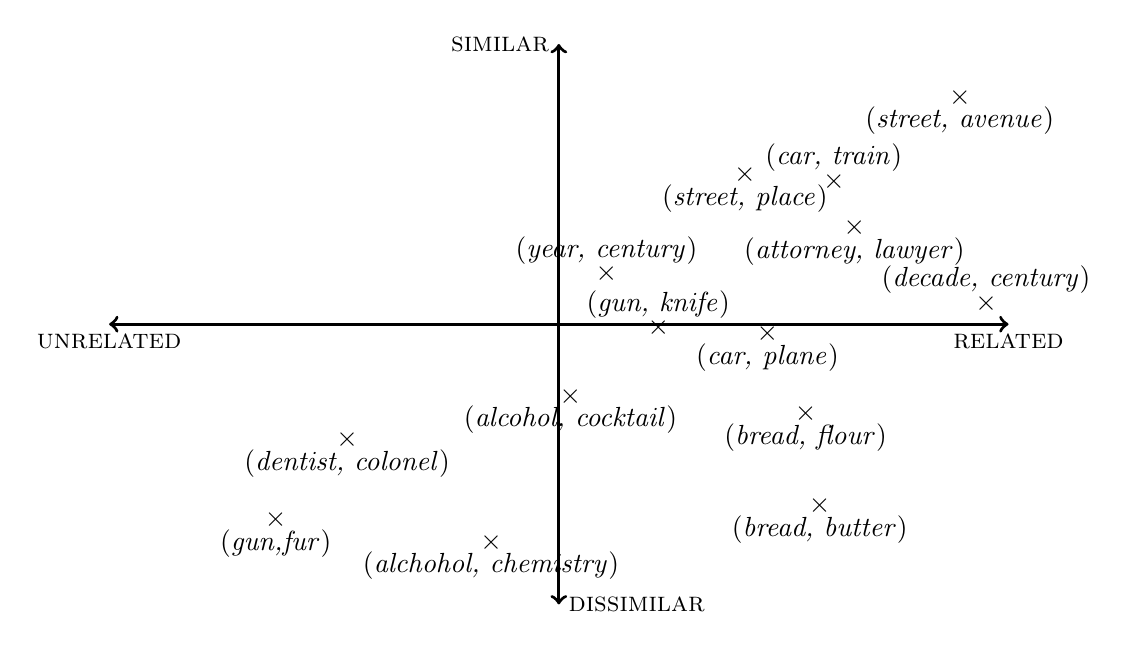
\begin{tikzpicture}
    \begin{axis}[xscale=2,yscale=1.5,hide axis]
      \addplot [<->,very thick] coordinates{(0,5) (10,5)};
      \addplot [<->,very thick] coordinates{(5,0) (5,10)};
      \node at (axis cs: 0,5) [below] {\normalsize \textsc{unrelated}};
      \node at (axis cs: 10,5) [below] {\normalsize \textsc{related}};
      \node at (axis cs: 5,0) [right] {\normalsize \textsc{dissimilar}};
      \node at (axis cs: 5,10) [left] {\normalsize \textsc{similar}};
      \node at (axis cs: 7.901,1.760) [below] {(\emph{bread, butter})};
      \node at (axis cs: 7.901,1.760) {$\times$};
      \node at (axis cs: 2.646,2.940) [below] {(\emph{dentist, colonel})};
      \node at (axis cs: 2.646,2.940) {$\times$};
      \node at (axis cs: 4.247,1.109) [below] {(\emph{alchohol, chemistry})};
      \node at (axis cs: 4.247,1.109) {$\times$};
      \node at (axis cs: 7.744,3.406) [below] {(\emph{bread, flour})};
      \node at (axis cs: 7.744,3.406) {$\times$};
      \node at (axis cs: 5.129,3.714) [below] {(\emph{alcohol, cocktail})};
      \node at (axis cs: 5.129,3.714) {$\times$};
      \node at (axis cs: 5.530,5.901) [above] {(\emph{year, century})};
      \node at (axis cs: 5.530,5.901) {$\times$};
      \node at (axis cs: 9.75,5.368) [above] {(\emph{decade, century})};
      \node at (axis cs: 9.75,5.368) {$\times$};
      \node at (axis cs: 7.320,4.828) [below] {(\emph{car, plane})};
      \node at (axis cs: 7.320,4.828) {$\times$};
      \node at (axis cs: 8.057,7.550) [above] {(\emph{car, train})};
      \node at (axis cs: 8.057,7.550) {$\times$};
      \node at (axis cs: 8.286,6.724) [below] {(\emph{attorney, lawyer})};
      \node at (axis cs: 8.286,6.724) {$\times$};
      \node at (axis cs: 1.852,1.512) [below] {(\emph{gun,fur})};
      \node at (axis cs: 1.852,1.512) {$\times$};
      \node at (axis cs: 6.106,4.936) [above] {(\emph{gun, knife})};
      \node at (axis cs: 6.106,4.936) {$\times$};
      \node at (axis cs: 7.068,7.667) [below] {(\emph{street, place})};
      \node at (axis cs: 7.068,7.667) {$\times$};
      \node at (axis cs: 9.458,9.050) [below] {(\emph{street, avenue})};
      \node at (axis cs: 9.458,9.050) {$\times$};
    \end{axis}
  \end{tikzpicture}
\caption[Axes of Relatedness and Similarity]{Noun pair scores along axes of relatedness and similarity as returned by a model built from features of 2x2 word co-occurrence window, 400 dimensional, \textsc{indy} type subspaces.}
\label{fig:axes}
\end{figure}

Putting aside for a moment the analysis of individual features, the overall import of this comparison is to a certain extent the vindication of the hypothesis that different features are predictive of relatedness versus similarity.\footnote{Intriguingly, when identical words are given as input, they are rated as being very related and very dissimilar.  The latter outcome is obviously an imperfection, but it also reveals the extent to which the models of each type of semantic phenomenon are making use of different geometric features, or the same features in opposite ways.}  This is illustrated in Figure~\ref{fig:axes}, where a selection of word pairs from both the WordSim and SimLex datasets are projected along axes of relatedness and similarity based on the outputs of the respective models learned based on the geometric features of 2x2 word window, 400 dimensional \textsc{indy} subspaces.  \revAK{2}{These pairs have been selected to illustrate model outputs at a range of different levels for both relatedness and similarity, additionally comparing single words across different pairs where possible in order to see how model output changes as one component of input shifts.}  So, for instance, \emph{bread} is considered fairly related but not at all similar to \emph{butter}; \emph{flour} is rated as being about equally related to \emph{bread} as \emph{butter}, but somewhat more similar.  Similar trends are observed in the progress from (\emph{car, plane}) to (\emph{car, train}) and (\emph{alcohol, chemistry}) to (\emph{alcohol, cocktail}).  Meanwhile, and perhaps less explicably, \emph{year} and \emph{decade} are about equally similar to \emph{century}, but \emph{decade} is modelled as being considerably more related.  The emptiness of the upper-left region of the field in this selection is characteristic of the models overall: words that are similar are in general \emph{de facto} related to one another, but \emph{relatedness} does not conversely predict similarity.

Figure~\ref{fig:relsimspaces} presents an assortment of two dimensional renderings of three dimensional projections of 400 dimensional subspaces chosen from across the spectrum of both similarity and relatedness ratings as returned by the \textsc{indy} technique operating on the 2x2 word window base space\revAK{2}{, focussing on selections of word pairs from the various extents of Figure~\ref{fig:axes}}.  The projection to three dimensions preserves the distance of the word-vectors and the generic vectors from the origin, as well as the angles between each vector, keeping the centroid vector $C$ in the centre of the positive region of the space.  It should also be noted that the norm of the vector $X$ is scaled by a factor of 0.5 for the sake of visibility.  The objective of these renderings is to offer an impression of the shifts in the overall comportment of the statistical geometry of subspaces moving along axes of both relatedness and similarity.

\begin{figure}
\footnotesize
\begin{subfigure}{0.3\textwidth} % bread - butter
\centering
  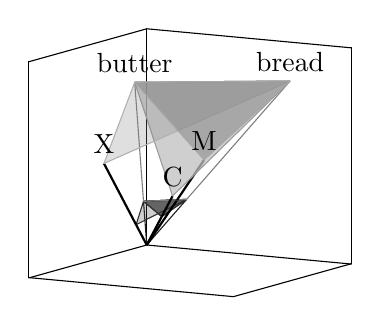
\begin{tikzpicture}
    \def\varA{(0.4845,70.1031,81.8944)};
    \def\varB{(62.7253,30.3505,87.3224)};
    \def\varC{(29.7558,29.7557,29.7557)};
    \def\varM{(10.9901,34.2885,43.9946)};
    \def\varX{(100.0506,36.9228,56.1392)};
    \def\varAN{(0.1348,19.5088,22.7901)};
    \def\varBN{(16.8439,8.1502,23.4491)};
    \def\varCN{(17.3205,17.3205,17.3205)};
    \def\varMN{(5.7994,18.0940,23.2158)};
    \def\varXN{(24.9048,9.1909,13.9743)};
    \def\nodA{0.4845,70.1031,81.8944};
    \def\nodB{62.7253,30.3505,87.3224};
    \def\nodC{29.7558,29.7557,29.7557};
    \def\nodM{10.9901,34.2885,43.9946};
    \def\nodX{100.0506,36.9228,56.1392};
    \begin{axis}[scale = 0.6,axis line style=white,view={120}{10},xmin=0,xmax=100,ymin=0,ymax=100,zmin=0,zmax=100,colormap/blackwhite,ticks=none]
      \addplot3[color=black,thick] coordinates {(0,0,100) (0,100,100)};
      \addplot3[color=black,thick] coordinates {(0,0,100) (100,0,100)};
      \addplot3[color=black,thick] coordinates {(0,100,0) (0,100,100)};
      \addplot3[color=black,thick] coordinates {(0,100,0) (100,100,0)};
      \addplot3[color=black,thick] coordinates {(100,0,0) (100,0,100)};
      \addplot3[color=black,thick] coordinates {(100,0,0) (100,100,0)};
      \addplot3[color=black] coordinates {(0,0,0) (0,0,100)};
      \addplot3[color=black] coordinates {(0,0,0) (0,100,0)};
      \addplot3[color=black] coordinates {(0,0,0) (100,0,0)};
      \addplot3[patch,patch type=triangle,color=gray,fill opacity=0.0] coordinates {(0.0,0.0,0.0) \varCN \varAN};
      \addplot3[patch,patch type=triangle,color=gray,fill opacity=0.0] coordinates {(0.0,0.0,0.0) \varCN \varBN};
      \addplot3[patch,patch type=triangle,color=darkgray,fill opacity=0.75] coordinates {\varCN \varAN \varBN};
      \addplot3[patch,patch type=triangle,color=darkgray,fill opacity=0.5] coordinates {\varMN \varAN \varBN};
      \addplot3[patch,patch type=triangle,color=darkgray,fill opacity=0.25] coordinates {\varXN \varAN \varBN};
      \addplot3 [color=black,thick] coordinates {(0,0,0) \varCN};
      \addplot3 [color=black,thick] coordinates {(0,0,0) \varXN};
      \addplot3 [color=black,thick] coordinates {(0,0,0) \varMN};
      \addplot3 [patch,patch type=rectangle,color=lightgray,fill opacity=0.0] coordinates{\varAN \varA \varB \varBN
};
      \addplot3 [color=black,thick] coordinates {\varCN \varC};
      \addplot3 [color=black,thick] coordinates {\varXN \varX};
      \addplot3 [color=black,thick] coordinates {\varMN \varM};
      \addplot3 [patch,patch type=triangle,color=lightgray,fill opacity=0.75] coordinates{\varA \varC \varB};
      \addplot3 [patch,patch type=triangle,color=gray,fill opacity=0.25] coordinates{\varA \varX \varB};
      \addplot3 [patch,patch type=triangle,color=gray,fill opacity=0.5] coordinates{\varA \varM \varB};
      \node [anchor=south] at (axis cs: \nodA) {bread};
      \node [anchor=south] at (axis cs: \nodB) {butter};
      \node [anchor=south] at (axis cs: \nodC) {C};
      \node [anchor=south] at (axis cs: \nodX) {X};
      \node [anchor=south] at (axis cs: \nodM) {M};
    \end{axis}
  \end{tikzpicture}
\caption*{\footnotesize \emph{relatedness = 7.901} \\ \emph{similarity = 1.760}}
\end{subfigure}
\hfill
\begin{subfigure}{0.3\textwidth} % car - plane
\centering
  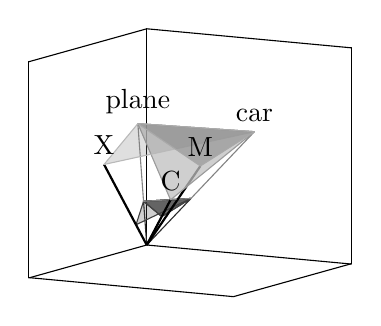
\begin{tikzpicture}
    \def\varA{(-9.246,47.099,55.012)};
    \def\varB{(46.777,22.683,65.128)};
    \def\varC{(27.435,27.435,27.434)};
    \def\varM{(9.784,31.783,40.743)};
    \def\varX{(99.192,36.477,55.514)};
    \def\varAN{(-3.799,19.354,22.605)};
    \def\varBN{(16.840,8.166,23.446)};
    \def\varCN{(17.321,17.321,17.320)};
    \def\varMN{(5.581,18.130,23.241)};
    \def\varXN{(24.927,9.167,13.951)};
    \def\nodA{-9.246,47.099,55.012};
    \def\nodB{46.777,22.683,65.128};
    \def\nodC{27.435,27.435,27.434};
    \def\nodM{9.784,31.783,40.743};
    \def\nodX{99.192,36.477,55.514};
    \begin{axis}[scale = 0.6,axis line style=white,view={120}{10},xmin=0,xmax=100,ymin=0,ymax=100,zmin=0,zmax=100,colormap/blackwhite,ticks=none]
      \addplot3[color=black,thick] coordinates {(0,0,100) (0,100,100)};
      \addplot3[color=black,thick] coordinates {(0,0,100) (100,0,100)};
      \addplot3[color=black,thick] coordinates {(0,100,0) (0,100,100)};
      \addplot3[color=black,thick] coordinates {(0,100,0) (100,100,0)};
      \addplot3[color=black,thick] coordinates {(100,0,0) (100,0,100)};
      \addplot3[color=black,thick] coordinates {(100,0,0) (100,100,0)};
      \addplot3[color=black] coordinates {(0,0,0) (0,0,100)};
      \addplot3[color=black] coordinates {(0,0,0) (0,100,0)};
      \addplot3[color=black] coordinates {(0,0,0) (100,0,0)};
      \addplot3[patch,patch type=triangle,color=gray,fill opacity=0.0] coordinates {(0.0,0.0,0.0) \varCN \varAN};
      \addplot3[patch,patch type=triangle,color=gray,fill opacity=0.0] coordinates {(0.0,0.0,0.0) \varCN \varBN};
      \addplot3[patch,patch type=triangle,color=darkgray,fill opacity=0.75] coordinates {\varCN \varAN \varBN};
      \addplot3[patch,patch type=triangle,color=darkgray,fill opacity=0.5] coordinates {\varMN \varAN \varBN};
      \addplot3[patch,patch type=triangle,color=darkgray,fill opacity=0.25] coordinates {\varXN \varAN \varBN};
      \addplot3 [color=black,thick] coordinates {(0,0,0) \varCN};
      \addplot3 [color=black,thick] coordinates {(0,0,0) \varXN};
      \addplot3 [color=black,thick] coordinates {(0,0,0) \varMN};
      \addplot3 [patch,patch type=rectangle,color=lightgray,fill opacity=0.0] coordinates{\varAN \varA \varB \varBN
};
      \addplot3 [color=black,thick] coordinates {\varCN \varC};
      \addplot3 [color=black,thick] coordinates {\varXN \varX};
      \addplot3 [color=black,thick] coordinates {\varMN \varM};
      \addplot3 [patch,patch type=triangle,color=lightgray,fill opacity=0.75] coordinates{\varA \varC \varB};
      \addplot3 [patch,patch type=triangle,color=gray,fill opacity=0.25] coordinates{\varA \varX \varB};
      \addplot3 [patch,patch type=triangle,color=gray,fill opacity=0.5] coordinates{\varA \varM \varB};
      \node [anchor=south] at (axis cs: \nodA) {car};
      \node [anchor=south] at (axis cs: \nodB) {plane};
      \node [anchor=south] at (axis cs: \nodC) {C};
      \node [anchor=south] at (axis cs: \nodX) {X};
      \node [anchor=south] at (axis cs: \nodM) {M};
    \end{axis}
  \end{tikzpicture}
\caption*{\footnotesize \emph{relatedness = 7.320} \\ \emph{similarity = 4.828}}
\end{subfigure}
\hfill
\begin{subfigure}{0.3\textwidth} % car - train
\centering
  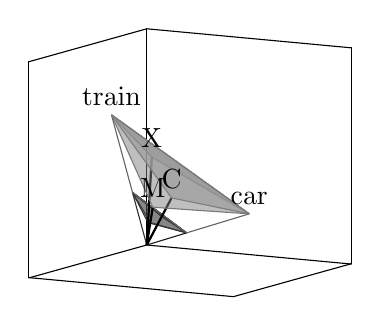
\begin{tikzpicture}
    \def\varA{(29.3619,66.8752,24.7492)};
    \def\varB{(34.8883,2.9505,65.6366)};
    \def\varC{(28.6170,28.6166,28.6169)};
    \def\varM{(36.6335,24.0788,25.1374)};
    \def\varX{(87.7695,53.1711,58.6364)};
    \def\varAN{(11.4224,26.0159,9.6280)};
    \def\varBN{(14.0695,1.1898,26.4695)};
    \def\varCN{(17.3206,17.3204,17.3206)};
    \def\varMN{(21.7478,14.2946,14.9230)};
    \def\varXN{(22.2784,13.4963,14.8836)};
    \def\nodA{29.3619,66.8752,24.7492};
    \def\nodB{34.8883,2.9505,65.6366};
    \def\nodC{28.6170,28.6166,28.6169};
    \def\nodM{36.6335,24.0788,25.1374};
    \def\nodX{87.7695,53.1711,58.6364};
    \begin{axis}[scale = 0.6,axis line style=white,view={120}{10},xmin=0,xmax=100,ymin=0,ymax=100,zmin=0,zmax=100,colormap/blackwhite,ticks=none]
      \addplot3[color=black,thick] coordinates {(0,0,100) (0,100,100)};
      \addplot3[color=black,thick] coordinates {(0,0,100) (100,0,100)};
      \addplot3[color=black,thick] coordinates {(0,100,0) (0,100,100)};
      \addplot3[color=black,thick] coordinates {(0,100,0) (100,100,0)};
      \addplot3[color=black,thick] coordinates {(100,0,0) (100,0,100)};
      \addplot3[color=black,thick] coordinates {(100,0,0) (100,100,0)};
      \addplot3[color=black] coordinates {(0,0,0) (0,0,100)};
      \addplot3[color=black] coordinates {(0,0,0) (0,100,0)};
      \addplot3[color=black] coordinates {(0,0,0) (100,0,0)};
      \addplot3[patch,patch type=triangle,color=gray,fill opacity=0.0] coordinates {(0.0,0.0,0.0) \varCN \varAN};
      \addplot3[patch,patch type=triangle,color=gray,fill opacity=0.0] coordinates {(0.0,0.0,0.0) \varCN \varBN};
      \addplot3[patch,patch type=triangle,color=darkgray,fill opacity=0.75] coordinates {\varCN \varAN \varBN};
      \addplot3[patch,patch type=triangle,color=darkgray,fill opacity=0.5] coordinates {\varMN \varAN \varBN};
      \addplot3[patch,patch type=triangle,color=darkgray,fill opacity=0.25] coordinates {\varXN \varAN \varBN};
      \addplot3 [color=black,thick] coordinates {(0,0,0) \varCN};
      \addplot3 [color=black,thick] coordinates {(0,0,0) \varXN};
      \addplot3 [color=black,thick] coordinates {(0,0,0) \varMN};
      \addplot3 [patch,patch type=rectangle,color=lightgray,fill opacity=0.0] coordinates{\varAN \varA \varB \varBN
};
      \addplot3 [color=black,thick] coordinates {\varCN \varC};
      \addplot3 [color=black,thick] coordinates {\varXN \varX};
      \addplot3 [color=black,thick] coordinates {\varMN \varM};
      \addplot3 [patch,patch type=triangle,color=lightgray,fill opacity=0.75] coordinates{\varA \varC \varB};
      \addplot3 [patch,patch type=triangle,color=gray,fill opacity=0.25] coordinates{\varA \varX \varB};
      \addplot3 [patch,patch type=triangle,color=gray,fill opacity=0.5] coordinates{\varA \varM \varB};
      \node [anchor=south] at (axis cs: \nodA) {car};
      \node [anchor=south] at (axis cs: \nodB) {train};
      \node [anchor=south] at (axis cs: \nodC) {C};
      \node [anchor=south] at (axis cs: \nodX) {X};
      \node [anchor=south] at (axis cs: \nodM) {M};
    \end{axis}
  \end{tikzpicture}
\caption*{\footnotesize \emph{relatedness = 8.057} \\ \emph{similarity = 7.550}}
\end{subfigure}
\vfill
\vspace{10pt}
\vfill
\begin{subfigure}{0.3\textwidth} % dentist - colonel
\centering
  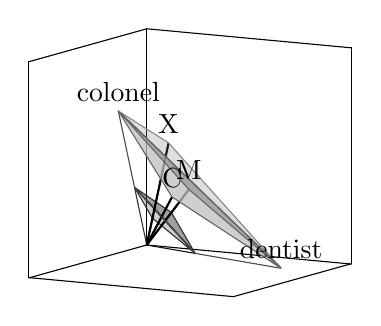
\begin{tikzpicture}
    \def\varA{(24.4577,79.6073,0.0101)};
    \def\varB{(23.9986,0.0101,65.5099)};
    \def\varC{(29.1739,29.1740,29.1738)};
    \def\varM{(22.2100,33.3543,31.9578)};
    \def\varX{(77.1030,55.1488,63.7419)};
    \def\varAN{(8.8105,28.6771,0.0036)};
    \def\varBN{(10.3194,0.0043,28.1693)};
    \def\varCN{(17.3205,17.3206,17.3205)};
    \def\varMN{(12.9996,19.5225,18.7051)};
    \def\varXN{(20.2488,14.4832,16.7399)};
    \def\nodA{24.4577,79.6073,0.0101};
    \def\nodB{23.9986,0.0101,65.5099};
    \def\nodC{29.1739,29.1740,29.1738};
    \def\nodM{22.2100,33.3543,31.9578};
    \def\nodX{77.1030,55.1488,63.7419};
    \begin{axis}[scale = 0.6,axis line style=white,view={120}{10},xmin=0,xmax=100,ymin=0,ymax=100,zmin=0,zmax=100,colormap/blackwhite,ticks=none]
      \addplot3[color=black,thick] coordinates {(0,0,100) (0,100,100)};
      \addplot3[color=black,thick] coordinates {(0,0,100) (100,0,100)};
      \addplot3[color=black,thick] coordinates {(0,100,0) (0,100,100)};
      \addplot3[color=black,thick] coordinates {(0,100,0) (100,100,0)};
      \addplot3[color=black,thick] coordinates {(100,0,0) (100,0,100)};
      \addplot3[color=black,thick] coordinates {(100,0,0) (100,100,0)};
      \addplot3[color=black] coordinates {(0,0,0) (0,0,100)};
      \addplot3[color=black] coordinates {(0,0,0) (0,100,0)};
      \addplot3[color=black] coordinates {(0,0,0) (100,0,0)};
      \addplot3[patch,patch type=triangle,color=gray,fill opacity=0.0] coordinates {(0.0,0.0,0.0) \varCN \varAN};
      \addplot3[patch,patch type=triangle,color=gray,fill opacity=0.0] coordinates {(0.0,0.0,0.0) \varCN \varBN};
      \addplot3[patch,patch type=triangle,color=darkgray,fill opacity=0.75] coordinates {\varCN \varAN \varBN};
      \addplot3[patch,patch type=triangle,color=darkgray,fill opacity=0.5] coordinates {\varMN \varAN \varBN};
      \addplot3[patch,patch type=triangle,color=darkgray,fill opacity=0.25] coordinates {\varXN \varAN \varBN};
      \addplot3 [color=black,thick] coordinates {(0,0,0) \varCN};
      \addplot3 [color=black,thick] coordinates {(0,0,0) \varXN};
      \addplot3 [color=black,thick] coordinates {(0,0,0) \varMN};
      \addplot3 [patch,patch type=rectangle,color=lightgray,fill opacity=0.0] coordinates{\varAN \varA \varB \varBN
};
      \addplot3 [color=black,thick] coordinates {\varCN \varC};
      \addplot3 [color=black,thick] coordinates {\varXN \varX};
      \addplot3 [color=black,thick] coordinates {\varMN \varM};
      \addplot3 [patch,patch type=triangle,color=lightgray,fill opacity=0.75] coordinates{\varA \varC \varB};
      \addplot3 [patch,patch type=triangle,color=gray,fill opacity=0.25] coordinates{\varA \varX \varB};
      \addplot3 [patch,patch type=triangle,color=gray,fill opacity=0.5] coordinates{\varA \varM \varB};
      \node [anchor=south] at (axis cs: \nodA) {dentist};
      \node [anchor=south] at (axis cs: \nodB) {colonel};
      \node [anchor=south] at (axis cs: \nodC) {C};
      \node [anchor=south] at (axis cs: \nodX) {X};
      \node [anchor=south] at (axis cs: \nodM) {M};
    \end{axis}
  \end{tikzpicture}
\caption*{\footnotesize \emph{relatedness = 2.646} \\ \emph{similarity = 2.940}}
\end{subfigure}
\hfill
\begin{subfigure}{0.3\textwidth} % alcohol - cocktail
\centering
  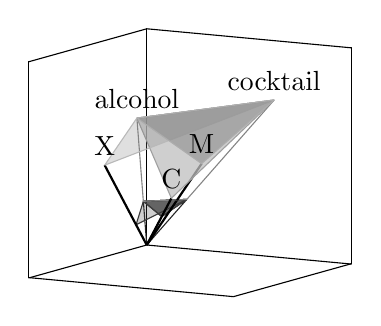
\begin{tikzpicture}
    \def\varA{(0.0441,62.0809,72.3646)};
    \def\varB{(48.9838,23.4812,68.0899)};
    \def\varC{(28.4173,28.4167,28.4161)};
    \def\varM{(10.4545,32.7756,42.0257)};
    \def\varX{(98.1159,36.1570,54.9788)};
    \def\varAN{(0.0139,19.5336,22.7693)};
    \def\varBN{(16.8709,8.0873,23.4514)};
    \def\varCN{(17.3209,17.3205,17.3202)};
    \def\varMN{(5.7748,18.1044,23.2139)};
    \def\varXN{(24.9155,9.1817,13.9613)};
    \def\nodA{0.0441,62.0809,72.3646};
    \def\nodB{48.9838,23.4812,68.0899};
    \def\nodC{28.4173,28.4167,28.4161};
    \def\nodM{10.4545,32.7756,42.0257};
    \def\nodX{98.1159,36.1570,54.9788};
    \begin{axis}[scale = 0.6,axis line style=white,view={120}{10},xmin=0,xmax=100,ymin=0,ymax=100,zmin=0,zmax=100,colormap/blackwhite,ticks=none]
      \addplot3[color=black,thick] coordinates {(0,0,100) (0,100,100)};
      \addplot3[color=black,thick] coordinates {(0,0,100) (100,0,100)};
      \addplot3[color=black,thick] coordinates {(0,100,0) (0,100,100)};
      \addplot3[color=black,thick] coordinates {(0,100,0) (100,100,0)};
      \addplot3[color=black,thick] coordinates {(100,0,0) (100,0,100)};
      \addplot3[color=black,thick] coordinates {(100,0,0) (100,100,0)};
      \addplot3[color=black] coordinates {(0,0,0) (0,0,100)};
      \addplot3[color=black] coordinates {(0,0,0) (0,100,0)};
      \addplot3[color=black] coordinates {(0,0,0) (100,0,0)};
      \addplot3[patch,patch type=triangle,color=gray,fill opacity=0.0] coordinates {(0.0,0.0,0.0) \varCN \varAN};
      \addplot3[patch,patch type=triangle,color=gray,fill opacity=0.0] coordinates {(0.0,0.0,0.0) \varCN \varBN};
      \addplot3[patch,patch type=triangle,color=darkgray,fill opacity=0.75] coordinates {\varCN \varAN \varBN};
      \addplot3[patch,patch type=triangle,color=darkgray,fill opacity=0.5] coordinates {\varMN \varAN \varBN};
      \addplot3[patch,patch type=triangle,color=darkgray,fill opacity=0.25] coordinates {\varXN \varAN \varBN};
      \addplot3 [color=black,thick] coordinates {(0,0,0) \varCN};
      \addplot3 [color=black,thick] coordinates {(0,0,0) \varXN};
      \addplot3 [color=black,thick] coordinates {(0,0,0) \varMN};
      \addplot3 [patch,patch type=rectangle,color=lightgray,fill opacity=0.0] coordinates{\varAN \varA \varB \varBN
};
      \addplot3 [color=black,thick] coordinates {\varCN \varC};
      \addplot3 [color=black,thick] coordinates {\varXN \varX};
      \addplot3 [color=black,thick] coordinates {\varMN \varM};
      \addplot3 [patch,patch type=triangle,color=lightgray,fill opacity=0.75] coordinates{\varA \varC \varB};
      \addplot3 [patch,patch type=triangle,color=gray,fill opacity=0.25] coordinates{\varA \varX \varB};
      \addplot3 [patch,patch type=triangle,color=gray,fill opacity=0.5] coordinates{\varA \varM \varB};
      \node [anchor=south] at (axis cs: \nodA) {cocktail};
      \node [anchor=south] at (axis cs: \nodB) {alcohol};
      \node [anchor=south] at (axis cs: \nodC) {C};
      \node [anchor=south] at (axis cs: \nodX) {X};
      \node [anchor=south] at (axis cs: \nodM) {M};
    \end{axis}
  \end{tikzpicture}
\caption*{\footnotesize \emph{relatedness = 5.129} \\ \emph{similarity = 3.714}}
\end{subfigure}
\hfill
\begin{subfigure}{0.3\textwidth} % bread - flour
\centering
  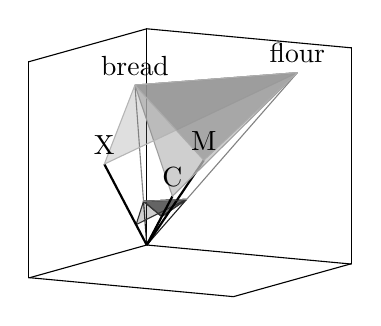
\begin{tikzpicture}
    \def\varA{(0.5080,73.6638,86.0712)};
    \def\varB{(61.6190,29.8353,85.7887)};
    \def\varC{(29.6193,29.6192,29.6193)};
    \def\varM{(10.9373,34.1320,43.7940)};
    \def\varX{(99.2437,36.6311,55.6956)};
    \def\varAN{(0.1345,19.5065,22.7921)};
    \def\varBN{(16.8423,8.1549,23.4486)};
    \def\varCN{(17.3205,17.3205,17.3205)};
    \def\varMN{(5.7981,18.0941,23.2161)};
    \def\varXN{(24.9035,9.1919,13.9759)};
    \def\nodA{0.5080,73.6638,86.0712};
    \def\nodB{61.6190,29.8353,85.7887};
    \def\nodC{29.6193,29.6192,29.6193};
    \def\nodM{10.9373,34.1320,43.7940};
    \def\nodX{99.2437,36.6311,55.6956};
    \begin{axis}[scale = 0.6,axis line style=white,view={120}{10},xmin=0,xmax=100,ymin=0,ymax=100,zmin=0,zmax=100,colormap/blackwhite,ticks=none]
      \addplot3[color=black,thick] coordinates {(0,0,100) (0,100,100)};
      \addplot3[color=black,thick] coordinates {(0,0,100) (100,0,100)};
      \addplot3[color=black,thick] coordinates {(0,100,0) (0,100,100)};
      \addplot3[color=black,thick] coordinates {(0,100,0) (100,100,0)};
      \addplot3[color=black,thick] coordinates {(100,0,0) (100,0,100)};
      \addplot3[color=black,thick] coordinates {(100,0,0) (100,100,0)};
      \addplot3[color=black] coordinates {(0,0,0) (0,0,100)};
      \addplot3[color=black] coordinates {(0,0,0) (0,100,0)};
      \addplot3[color=black] coordinates {(0,0,0) (100,0,0)};
      \addplot3[patch,patch type=triangle,color=gray,fill opacity=0.0] coordinates {(0.0,0.0,0.0) \varCN \varAN};
      \addplot3[patch,patch type=triangle,color=gray,fill opacity=0.0] coordinates {(0.0,0.0,0.0) \varCN \varBN};
      \addplot3[patch,patch type=triangle,color=darkgray,fill opacity=0.75] coordinates {\varCN \varAN \varBN};
      \addplot3[patch,patch type=triangle,color=darkgray,fill opacity=0.5] coordinates {\varMN \varAN \varBN};
      \addplot3[patch,patch type=triangle,color=darkgray,fill opacity=0.25] coordinates {\varXN \varAN \varBN};
      \addplot3 [color=black,thick] coordinates {(0,0,0) \varCN};
      \addplot3 [color=black,thick] coordinates {(0,0,0) \varXN};
      \addplot3 [color=black,thick] coordinates {(0,0,0) \varMN};
      \addplot3 [patch,patch type=rectangle,color=lightgray,fill opacity=0.0] coordinates{\varAN \varA \varB \varBN
};
      \addplot3 [color=black,thick] coordinates {\varCN \varC};
      \addplot3 [color=black,thick] coordinates {\varXN \varX};
      \addplot3 [color=black,thick] coordinates {\varMN \varM};
      \addplot3 [patch,patch type=triangle,color=lightgray,fill opacity=0.75] coordinates{\varA \varC \varB};
      \addplot3 [patch,patch type=triangle,color=gray,fill opacity=0.25] coordinates{\varA \varX \varB};
      \addplot3 [patch,patch type=triangle,color=gray,fill opacity=0.5] coordinates{\varA \varM \varB};
      \node [anchor=south] at (axis cs: \nodA) {flour};
      \node [anchor=south] at (axis cs: \nodB) {bread};
      \node [anchor=south] at (axis cs: \nodC) {C};
      \node [anchor=south] at (axis cs: \nodX) {X};
      \node [anchor=south] at (axis cs: \nodM) {M};
    \end{axis}
  \end{tikzpicture}
\caption*{\footnotesize \emph{relatedness = 7.744} \\ \emph{similarity = 3.406}}
\end{subfigure}
\caption[The Geometry of Relatedness and Similarity]{Subspaces, including word-vectors and generic features, derived from word pairs with an assortment of relatedness and similarity scores.}
\label{fig:relsimspaces}
\end{figure}

Moving up the scale of similarity from (\emph{butter, bread}) to (\emph{plane, car}), we can observe a tightening of the angle between the word-vectors and a general contracting of the space, followed by an increase in the span between the word-vectors as we ratchet our way up to the highly similar (\emph{train, car}).  An almost opposite effect can be observed, on the other hand, as relatedness increases from (\emph{alcohol, cocktail}) to (\emph{bread, flour}), with the word-vectors themselves looming as the angle at $C$ contracts and the ratios of the distances to $M$ even out.  Perhaps the most interesting effect of all, though, is the visually evident similarity in the geometries of (\emph{colonel, dentist}), which are equivalently dissimilar and unrelated, and (\emph{train, car}), which are conversely highly similar and highly related: while my projection technique clearly struggles to accommodate the expanse of the angle between the unrelated word-vectors, the congruity of the characteristic spread of the various points in the spaces selected by the word-vectors is striking.  This raises an intriguing possibility that there may be a certain consistency in geometry based on the balance of similarity and relatedness, or, to put it differently, an indication that there is a certain shape to the statistics of a space in which similarity is the primary axis of relatedness, regardless of degree, versus a space in which there is some other specific semantic relationship in play.

\section{Frames of Similarity} \label{sec:frames}
\cite{Tversky1977}, in his psychologically motivated reflections on the geometry of similarity, observes that relationships of similarity are fundamentally not symmetric: there tends to be a preference to consider the specific more similar to the general, and the peripheral more similar to the prototypical, than the other way around.  So, to use Tversky's own example, \emph{ellipse} is more similar to \emph{circle} than \emph{circle} is to \emph{ellipse}; we might extend this conjecture to predict that \emph{wolf} is more similar to \emph{dog}, \emph{radiologist} more similar to \emph{doctor}, and \emph{limping} more similar to \emph{walking} than the converse propositions.  Indeed, the frequentist axiom extrapolated through the geometric analysis of the previous section, stating that more common words denote things that are more likely to generally be a component of a similarity relationship, is broadly in line with this observation.  Tversky makes the point that the conventional conditions of geometric relationships -- \emph{minimality}, \emph{symmetry}, and \emph{the triangle inequality} -- do not pertain in the case of similarity judgements, a point which if taken seriously serves to foil the project of static vector space models of word similarity.

\cite{ChenEA2017} carry this point forward experimentally, demonstrating that potential for the arbitrary construction of, for instance, analogies which demand geometrically impossible triangulations: to use one of their examples, \emph{nurse:patient::mother:baby} is a reasonable set of relationships, as is \emph{mother:baby::frog:tadpole}, but the proposition \emph{nurse:patient::frog:tadpole} seems obscure at best.  \citeauthor{ChenEA2017} demonstrate that human raters generally identify the failure of the third set of pairings in these types of triads, whereas standard distributional semantics including \texttt{word2vec} don't---in fact, they can't, since the semantic relationships in these models are represented as static distances.  The point that emerges here is that semantic relationship emerge within a certain frame of reference, and the reason that the analogy comparing nurses to frogs fails is because both the axis of \textsc{caring} that sustains the connection between nurses and mothers and the axis of \textsc{parentage} that connects mothers and frogs have dropped away.

The role of frames in theories of lexical semantics has already been mentioned in Chapter~\ref{sec:lexsem} and again earlier in this chapter.  To reiterate the point raised there, \cite{BarsalouEA1993} propose that cognition is organised in terms of frames allowing for a \emph{situated}, \emph{local} representation of concepts: a concept gains its structure through a situationally specific indexing of a variety of established models.  One of the consequences of this framework is that a concept emerges as the ``collection of all specialized models for a particular type of individual, together with their associated generic situations,'' (ibid, p. 48).  So, for instance, the concept \textsc{profession} contains models for constituents such as \textsc{dentist} and \textsc{attorney} and so forth, and the conceptual scheme is structured in such a way as to offer information about the situations which both independently and jointly pertain to the models associated with those constituents.  Inherent in this productive nesting of frames within frames and models in terms of their relationships to other models is the idea that concepts are specified in a particular cognitive context and generated on an \emph{ad hoc} basis.

These types of conceptual contexts are evident in the relatedness and similarity datasets which have been explored in this chapter.  In the SimLex data, for instance, (\emph{dentist}, \emph{colonel}) is rated as one of the least similar word pairs at 0.40, while (\emph{attorney}, \emph{lawyer}) is, at 9.25, considered one of the most similar pairs.  The difference seems reasonable enough in terms of a comparison between the two pairs, but the low rating of (\emph{dentist}, \emph{colonel}) leaves little room for either dentists or colonels to be even less similar to, say, \emph{gorilla}, or \emph{electricity}, or \emph{democracy}, and so forth.  What seems to be happening here is that human evaluators are identifying an implicit conceptual frame in which each word pair is to be evaluated: in the case of \emph{attorney}, \emph{lawyer}, \emph{dentist}, and \emph{colonel}, the frame is something like \textsc{profession}, and so the professional activities of colonels and dentists are judged to be more or less orthogonal, while attorneys and lawyers pursue very similar careers.  The inclusion of some additional comparison, for instance (\emph{dentist}, \emph{grandparent}), would suggest a broadening of the conceptual frame to something like \textsc{human}, and a corresponding drawing together of words denoting professions in particular.

Moreover, it is not particularly clear how a pair such as (\emph{dentist}, \emph{colonel}) should be considered either more or less similar to a pair like (\emph{gun}, \emph{fur}); the comparisons being made here seem just categorically different, and so the project of ranking the similarity of one above the other becomes a bit obscure.  Instead, the task at hand really seems to be to determine the conceptual domain in which the comparison is being made, and then to make an inherently relativistic judgement about the proximity of the denotations within the semantic space of that domain.  I suggest that my models are beginning to do this.  By taking a subset of co-occurrence dimensions expected to exhibit a degree of saliency for either or both of the words being analysed, a subspace with a certain degree of conceptual interpretability is generated.  So collectively, the 200 co-occurrence terms that are jointly most predictive of \emph{dentist} and \emph{colonel} also implicate \emph{lawyer} and \emph{attorney}, with those two words ranked 21 and 204 from the mean point of the input vectors respectively (out of a total vocabulary of 200,000), while when \emph{lawyer} and \emph{attorney} are used to generate a 200 dimensional subspace, \emph{dentist} comes in at 1,925 and \emph{colonel} at 1,096.

%EXAMPLES

What begins to emerge is something like a very rough version of the conceptual spaces described by \cite{Gardenfors2000}, in which regions of a space correspond to conceptual constituents and directions within regions can be interpreted as corresponding to values of properties that determine membership.  It must be emphasised that this comparison is at a general level of abstraction: my subspaces do not at this stage contain any of the nuanced attributional information of G\"{a}rdenfors's conceptual spaces, and my methodology generates unique subspaces for each word pair, so the scores returned by the models learned through linear regression are effectively comparisons between different, albeit potentially overlapping, subspaces.  Nonetheless, the reliably distinct respective predictors of relatedness and similarity within any given subspace suggest that there is already an element of conceptual structure at play in my models, even if it lacks much depth in terms of dimensional interpretation.

\cite{FaruquiEA2016} raise a number of issues with relatedness and similarity datasets, among them the uncertainty surrounding specific semantic phenomena and the lack of applicability of quantified word pair scores to practical NLP tasks.  Those authors ultimately propose that quantitative evaluations of vector space models of word meaning should avoid claims of generality, instead treating particular models as task specific implementations.  There is something to be said for this approach, and even more to be said in support of the effort to apply statistical NLP techniques to activities in other fields where heterogeneous data and contextual complexity present potentially confounding factors to the relatively abstract and rigid representational structures of distributional semantic models.  All the same, I maintain that word association tasks, particularly a battery of tasks spanning a variety of semantic phenomena, can be a valuable tool for exploring the capabilities of a methodology, and present the work that has been described in this chapter as a case in point.

A productive next step would be to develop methods targeting the classification of conceptual domains within which word pair comparisons are being performed, so, for instance, to identify that (\emph{dentist}, \emph{colonel}) and (\emph{attorney}, \emph{lawyer}) are both implicitly comparisons between \textsc{professions}, or at least are comparisons within the same unspecified domain.  Existing work in the field on conceptual entailment may prove helpful here: \cite{HerbelotEA2013}, for instance, use an entropic analysis of co-occurrence statistics to conjecture about hypernymy relationships between sets of words, while \cite{MelamudEA2014} use a method utilising syntagmatic co-occurrence information to model the probability of words belonging to the same semantic domain.  Equipped with an effective method for clustering relationships between words into conceptual domains, or alternatively for rating the degree of relevance inherent in a comparison between two relatedness judgements, my methodology offers, as has been demonstrated in the experiments reported above, a capacity for contextualising the relationships between representation in terms of co-occurrence dimensions and then discovering various geometric axes corresponding to different semantic properties.  As the words used as input to define a subspace become more related, the space itself likewise becomes more conceptually coherent, and I predict that these broadly semantic axes will take on a more narrowly G\"{a}rdenforsian characteristic, allowing for interpretation as properties specific to the concept implicit in the grouping.

The \textsc{indy} dimensional selection technique in particular would lend itself to this type of programmatic extension of research into semantic relatedness, as it facilitates the open-ended concatenation of dimensions from an analysis of an arbitrarily large set of constituent word-vectors (the \textsc{joint} and \textsc{indy} techniques, on the other hand, would presumably return increasingly uninteresting dimensions with universally non-zero values as the set of input words expands).  A subspace built using the \textsc{indy} technique based on an analysis of a set of words denoting, for instance, constituents of the concept \textsc{professionals} would acquire co-occurrence dimensions specifically salient to each of the input terms, and the construal of other word-vectors in the space along the collective profile of dimensions would, I forecast, be indicative of their conceptual situation according to the various properties of being a professional.  In such a space, we might predict that we would find, for instance, \emph{surgeon} somewhere in the vicinity of the region between \emph{barber} and \emph{butcher}

This proposition entails a major research project.  The data for establishing groups of conceptual relationships needs to be established, and the evaluation of a model's ability to capture the attributes giving these relationships structure presents a daunting task due to the open-endedness of conceptualisation itself.  Ultimately, questions of the validity of the assignment of properties to concepts, as they begin to reflect the modelling of situations in the world, are probably better suited for a qualitative analysis, and it is easy to imagine how this work might eventually lend itself to fruitful collaboration with fields such as educational studies and digital humanities.  For now I will leave this line of enquiry where it stands, with some promising results regarding the ability of my methodology to model the overlapping semantic phenomena of relatedness and similarity in a single space.  In the next chapter, I will explore my methodology's capacity for handling a broad and important set of semantic phenomena for which I believe it will be particularly well suited: figurative language.

%(for comparison, see where the pair (\emph{dentist, colonel}) falls in the space of Figure~\ref{fig:axes}, where it is one of the very few pairs considered to be marginally more similar than related)

\chapter{Metaphor and Coercion} \label{chap:figurative}
In this chapter, I will extend the empirical work on exploring the application of my context sensitive distributional semantic models to two semantic phenomena which involve the application of words in situations where their meanings are in some sense conceptually altered: \emph{metaphor} and \emph{semantic type coercion}.  The connotation of these terms will be explored throughout the course of this chapter, eventually arriving at a proposal for how to frame the idea of figurative language through a computational analysis.  As an overview, the distinguishing characteristic of these phenomena as they are conventionally understood is that they involve cases where what might be thought of as the stable, encyclopedic understanding of some word sense -- a \emph{dictionary definition} of a word, so to speak -- is in some way appropriated or subverted in order to, among other things, transfer information via the attributional conduits connecting figurative source to literal target.

My hypothesis is that, because figurative language always involves the contextual specification of word meaning, context sensitive geometries of lexical representations should provide an appropriate framework for identifying when this type of semantic phenomenon is in effect.  \cite{Fraser1993} demonstrates empirically that metaphor interpretation is, when a metaphor is presented to a subject out of context, an ambiguous exercise, and, to the extent that interpretations of de-contextualised metaphors can be predicted, the predicting factors are themselves culturally relative.  Along similar lines, \cite{BouveretEA2009} propose that metaphor production involves the contextual alignment of overlapping semantic frames, and that this alignment likewise imports structure associated with one frame into the domain of another, evident in, for instance, the additional transposition of syntactic constraints from source to target.  From a cognitive perspective, this coordinates a contextual theory of metaphor with the work on conceptual frames from \cite{Barsalou1992} discussed at the end of the previous chapter in the context of judgements of semantic similarity.  From a modelling perspective, this suggests that a methodology for projecting semantic spaces where contextualisation can reveal \emph{ad hoc} viewpoints on semantic relationships should be a productive approach to identifying figurative language.

The idea that metaphor and metonymy are both instances of ``a connection between two things where one term is substituted for another,'' \citep[][p. 260]{Gibbs1993} will quickly call to mind the premise of distributional semantics: if the motivation for building vector space models of word co-occurrence statistics is that related words have similar co-occurrence tendencies, then figurative language might be construed as a special case in which unrelated or at least conceptually divergent words are likewise sometimes found in similar sentential situations.  The question, then, is whether statistical characteristics of the particular co-occurrences profiles selected by words with different meanings are predictive of figurativeness.  A naive hypothesis might be that word combinations that are figurative should simply be further apart in a semantic space than word combination that are literal.  If related words have similar co-occurrence profiles, then maybe unrelated words, for instance words with different conceptual entailments, should have less similar co-occurrence profiles.  This conjecture, however, is belied first of all by the fact that, in the type of corpus containing a broad range of examples of language use necessary for building distributional semantic models, figurative language will already be built into the data \citep[and, as][has pointed out, figurative language is going to built into any sample of language no matter how small or basic]{Gibbs1994}.  A second problem is that, specifically to overcome the problems with modelling semantic relationships merely in terms of collocations, distributional semantics compares the co-occurrence profiles of words rather than their direct relationships, and it seems likely that word combinations prone to metaphoric interpretation might very well have at least overlapping profiles.

So the objective of the experiments reported in this chapter will be to explore the ways in which and the degrees to which a more fleshed out statistical description of contextually selected distributional semantic subspaces can reveal figurative language.  As with the experiments on relatedness and similarity reported in the previous chapter, in addition to the relationship between target word-vectors in the subspaces they select, the statistical properties of the selected dimensions themselves will also be examined.  And, again as with previous results, the instrument of analysis will be the geometric features of the subspaces in question, with, again, particular attention paid to the way in which the sets of features can collectively indicate figurative language.  The two primary datasets explored represent binary decisions about metaphoricity and coercion respectively, and so my models will be applied to classification tasks here.  In the case of metaphor, I also test whether a model learned based on classification data is generalisable to graduated human ratings of metaphoricity.  With the coercion data, I will examine whether the addition of information about sentential context enhances the classification of word pairs.  I will conclude the chapter with a reflection on some of the theoretical implications of the positive results attained here.

\section{An Experiment on Metaphor} \label{sec:metperiment}
As pointed out by \cite{ShutovaEA2013}, statistical approaches to metaphor identification and interpretation have generally been formulated in the context of the \emph{conceptual metaphor} theory of \cite{LakoffEA2003}.  This model is founded on the principle that ``we systematically use inference patterns from one conceptual domain to reason about another conceptual domain,'' (ibid, p. 246).  Metaphors are then the mechanism for performing the mapping between these domains, and as such cut right to the core of cognitive processes \citep{Gibbs1994}.  Statistical models of metaphor have accordingly treated metaphors as transformations of lexical representations, and vector space models of distributional semantics have naturally lent themselves to this type of approach.  The construction of representations with the potential to interact with one another in semantically productive ways has in turn lent itself to the development of models that consider the compositional nature of metaphor, effectively treating the metaphor itself as a transformation of the underlying representations.  So \cite{Utsumi2011} constructs candidate metaphor vectors by calculating the centroid of a number of vectors derived from an analysis of a noun-vector and a predicate-vector learned through latent semantic analysis, and then uses the spatial relationships between these composed vectors to analyse the metaphoricity of certain phrases.  \cite{HovyEA2013} similarly consider composition in their approach to metaphor classification, in this case by combining word-vector type representations with a model trained to identify metaphor based on dependency trees of sentences labelled for metaphoricity.

In the tradition of work on compositional distributional semantics explored by the likes of \cite{MitchellEA2010}, \cite{BaroniEA2010}, and \cite{CoeckeEA2011}, among others, semantic types such as adjectives and verbs are modelled as tensors which perform transformations on nouns, which are modelled as vectors.  In the normal run of things, compositional models therefore represent, for instance, noun phrases modified by adjectives as the product $A\overrightarrow{n}$, where $\overrightarrow{n}$ in a noun vector and $A$ is a matrix representing an adjective learned from observations of attested instances of the adjective with other noun word-vectors.  So the phrase \emph{black dog} becomes a word-vector in the same space as the representation of just \emph{dog}, and can be compared quantitatively and geometrically with other phrases such as \emph{white dog} or \emph{big cat} and so forth: these adjectival phrases become effectively denotations.  In the case of metaphor, these transformations are expected to map the word-vector representing metaphoric phrases into a region corresponding to the semantic domain of the original noun-vector modified by a metaphoric interpretation of the word associated with the tensor of a modifier or a predicate.  So, for instance, in a model that effectively captures metaphoricity, the composition of the vector space representations corresponding to \emph{brilliant light} would map to a region of space where comparisons between phrases like \emph{dark illumination} and \emph{red glow} are productive, while \emph{brilliant child} might be expected to map into the proximity of \emph{stupid boy} and \emph{boring girl}.\footnote{It should be noted that such a methodology at this point begins to assume dim shades of \citepos{Gardenfors2000} conceptual spaces, with different compositions inherently defining different regions of the space.}

\revJB{1}{Rather than using mathematically endowed informational structures to transform a lexical semantic representation from a literal to a metaphoric sense, my application of my context sensitive methodology will involve the identification of subspaces that capture the conceptual context facilitating a particular metaphor.  So, where }\cite{Utsumi2011} \rev{compounds input word-vectors to derive a metaphor vector, or where }\cite{GutierrezEA2016} \rev{derive tensors from an analysis of established metaphors in order to evaluate candidate metaphors, my approach involves, as with the work on relatedness and similarity described in the previous chapter, the projection of both source and target vectors into a contextualised subspace.  This means that the projected relationships between source and target do not capture, for instance, the transference of potentially atypical properties from one domain to another, and so one of my premises is that the identification of metaphor, that primary task that will be explored here, does not necessarily involve the interpretation of metaphor.  Instead, by discovering the characteristics of a subspace that is conducive to capturing the co-occurrences features collectively salient to the components of a metaphor, we are also effectively discovering how much work has to be done in order to find a profile of dimensions permitting an analysis of the words in question.  A hypothesis which will bear out in the following experiments is therefore that it is not only the relationship between projections of source and target vectors, but also the overall statistical situation of a given subspace that indicates the presence (and, potentially, degree) of metaphor.}  \revJB{2}{On the other hand, it must also be noted that my methodology will generally not be sensitive to the semantic nuances provided by highly localised contexts, so, for instance, the transference of a very particular property across the broader alignment of two conceptual domains.}

\subsection{Background and Data} \label{sec:metaback}
\revAK{10}{Some early computational approaches to metaphor maintained an essentially formal character:} \cite{vanGenabith2001} \revAK{10}{proposed a type theoretical model for describing metaphor, for instance.  Information processing approaches have, though, been by and large data-driven, understandably utilising the processing power of symbol manipulating machines---and these data-driven approaches have generally had some sort of connection with the cognitive linguistic stances on metaphor.  So, for instance,} \cite{ThomasEA1999} \revAK{10}{describe an information processing network which selectively projects features, inspired by the previously mentioned interaction view of metaphor developed by} \cite{Black1977}.  \revAK{10}{In terms of theoretical grounding,} \cite{Shutova2010} \revAK{10}{identifies the \emph{selectional preference violation} approach of} \cite{Wilks1978} \revAK{10}{as especially influential, perhaps because it was formulated specifically as an information processing mechanism.  A notable early effort from} \cite{Fass1991} \revAK{10}{is derived from this theoretical background, with correspondences in the selectional preferences of the arguments of verbs used to detect metonymic versus metaphoric uses of language.}

\revAK{10}{The mainstream of metaphor modelling has subsequently been characterised by symbol manipulating approaches and has  involved mapping between conceptual schemes} \citep{Indurkhya1997}, \revAK{10}{often domain specific, with the underlying assumption that mappings between domains correlate with the conceptual metaphor model} \citep{Narayanan1999}.  \revAK{10}{Typical symbolic approaches to metaphor modelling involve the construction of an ontology defined by features which can be mapped between elements.  The ATT-Meta system} \citep{LeeEA2001}, \revAK{10}{with its faculty for backchaining inferences across conceptual domains, is exemplary, and has furthermore been expanded into a metaphor generating system employing a combination of distributional semantic and incremental grammar techniques} \citep{GargettEA2013}.  \revAK{10}{ATT-Meta is particularly notable in that it applies systems of logic in the specific conceptual context of a metaphor it is handling} \citep{BarndenEA1999}, \revAK{10}{and in this respect is a symbolically grounded response to some of the same theoretical concerns that have motivated my own research.  Other symbolic approaches are notable for their recourse to pre-formulated knowledge bases such as WordNet} \citep{VealeEA2015}, \revAK{10}{or the web at large in conjunction with other resources} \citep{VealeEA2007}.

\revAK{10}{Symbolic approaches have tended to focus on the interpretation of metaphor by way of models of trans-conceptual mappings, but in another aspect of computational work, that of metaphor identification, statistical approaches have proved particularly effective.}\footnote{\cite{Shutova2013} \revAK{10}{suggests that computational identification and interpretation of metaphor, in line with psychological analysis, should be considered a joint task.}}  \revAK{10}{An early example is the TroFi model of} \cite{BirkeEA2006}, \revAK{10}{which uses a clustering algorithm trained on a set of tagged sample sentences to disambiguate between literal and non-literal verb use, followed by} \cite{Utsumi2011}, \revAK{10}{who explores clustering in the context of distributional semantics.  Indeed, many of these statistical approaches (see} \citealt{Dunn2013}; \citealt{TurneyEA2011} \revAK{10}{for a comparison of distributional semantic and symbolic models, and} \citealt{ShutovaEA2013} \revAK{10}{for an overview of statistical models in particular) have employed the techniques of distributional semantics, which will be discussed in the next section: here} \citepos{Kintsch2000} \revAK{10}{model of metaphoric interpretation as a contextually selective traversal of the space between word-vectors is seminal.  A notable recent instance of a statistical model for metaphor identification involving an application of compositional distributional semantics is described by} \cite{GutierrezEA2016}, \revAK{10}{of particular note here as the dataset presented by those authors will be used to evaluate the model at the heart of this thesis (see Chapter~\ref{chap:figurative} for a more detailed description).  Returning to the cognitive linguistic foundations of computational approaches to metaphor,} \cite{TsvetkovEA2014} \revAK{10}{go so far as to propose that their results derived from the statistical construction of what they construe as conceptual features associated with lexical representations ``support the hypothesis that metaphors are conceptual, rather than lexical, in nature,'' (ibid, p. 248).}

The data that I will use in this section to test my methodology was originally presented by \cite{GutierrezEA2016}, along with an accompanying experiment on a novel model.  It consists of 8,592 adjective-noun pairs, spanning 23 adjectives chosen for their membership in six different broad semantic categories that are prone to both literal and metaphoric use: so, for instance, \emph{bitter}, \emph{sour}, and \emph{sweet} are considered constituents of the category \textsc{taste}.  There are 3,473 different noun types used, with only 141 types, represented by 640 tokens, occurring in both literal and metaphoric phrases, hinting from the outset that some nouns might attract more metaphor than others.  Each pair has been rated as either literal or metaphoric by a pair of human annotators, with inter-annotator agreement measuring at Cohen's $\kappa = 0.80$; 4,593 of the pairs have been judged metaphorical.  This dataset was conceived as something of an expansion of the similar but smaller corpus of adjective-noun phrases annotated with binary metaphoricity classifications presented by \cite{TsvetkovEA2014} (and those authors tested their own data with an assortment of models, achieving highest f-scores by applying a random forest classifier to the features of an existing library of distributional semantic word-vectors).

In their own experimental treatment of the data, \citeauthor{GutierrezEA2016} constructed a pair of compositional models in the mode of \cite{BaroniEA2010}, learning adjective matrixes $A$ to map from noun-vectors to noun-adjective phrase-vectors extracted from observations of co-occurrences of both nouns and phrases in a corpus.  By creating separate tensor representations for literal and metaphoric instances of a given adjective, the authors can then compare the relationships between the vectors resulting from a noun-vector composed with literal and metaphoric senses of an adjective-vector to try to determine whether a given phrase would generally be classified as a metaphor or a literal expression by comparing the respective compared vectors to the phrase-vector as observed in the corpus.  In a further attempt to generalise the method, and, notably, to apply the conceptual metaphor theory of \cite{LakoffEA1980} to their computational model, the authors learn matrices performing linear transformations from literal to metaphoric adjective-noun compositions and then compare the similarity between observed phrase-vectors and literal composed vectors versus transformed literal composed vectors to determine whether a given phrase is metaphoric or not.

The data described by \citeauthor{GutierrezEA2016} will serve as the basis for testing my own context sensitive distributional semantic methodology's ability to classify phrases as literal or metaphoric, and the results of this experiment will be described in the following section.  My hypothesis is that metaphor, and indeed all figurative language, is fundamentally entangled with the context mutually indicated by the representations of the words participating in the composition being analysed.  In fact, I think that part of what is captured by the model described by \citeauthor{GutierrezEA2016}, and indeed a number of other researchers investigating statistical methods for metaphor classification, is precisely that there is a context inherent in the linear algebraic dynamics of composable lexical representations, and this is something which many researchers recognise.  But I also think that the explicit projection of context specific semantic subspaces, the mainstay of my methodology, should provide an ideal testing ground to discover the way in which statistical geometry can directly broadcast the presence or absence and even potentially the degree of metaphor inherent in a given phrase.  The following sections will test this hypothesis using a similar methodology to that applied to semantic relatedness and similarity in the previous chapter.  \revAK{1}{And, as with the results reported in the last chapter, different modelling techniques with similar dimensionality parameters will be compared for statistical significance, with results with $p < .01$ probability of random observation being considered significant.  In these cases, permutation tests generated through random shuffling of outputs will be used to generate empirical estimates, as outlined in Section~\ref{sec:methods}.}

%The section after that will explore the geometry of a particularly successful model learned using my methodology.  Finally, in Section~\ref{sec:genafor}, I will address the question of whether a classification model learned from the impressively large dataset contributed by \citeauthor{GutierrezEA2016} can be generalised to handle graduated human ratings of metaphoricity on a different type of metaphoric construction.

\subsection{Methodology and Results} \label{sec:metameth}
My own methodology is clearly less committed to maintaining distinct representations for different semantic types than the compositional models described above, instead modelling all words as untagged word-vectors based on their co-occurrences as observed across a large scale corpus.  This feature of my research is in part theoretically motivated: in line with \cite{Langacker1991}, and \emph{contra} the grammatic nativism or exceptionalism that has been foundational in theoretical linguistics, I would like to investigate the possiblity that ``grammar is fully and appropriately describable using only symbolic units, each having both semantic and phonological import,'' (ibid, p. 290).  In other words, the syntactic component of a natural language might be described in terms of the entanglements of the meaning-making structures -- the lexical semantic representations -- that arise in the course of language use, or maybe even as emergent properties of these entanglements.

With this in mind, I will approach the problem of metaphor classification with a similarly statistical and geometric methodology as was applied to relatedness and similarity in the previous chapter, outside of any \emph{prima fascie} model of syntax or compositionality.  For every pair of words in the data produced by \cite{GutierrezEA2016}, I generate subspaces of 20, 50, 200, and 400 dimensions using the \textsc{joint}, \textsc{indy}, and \textsc{zipped} techniques, projected from 2x2 and 5x5 word co-occurrence window base spaces.  This data specifies a distince role for each word, one being a metaphoric source (the adjective) and the other being a target (the noun): so, for instance, a \emph{bitter loss} is a loss, but presumably not one with an actual taste, and so the noun \emph{loss} co-opts something of the quality of bitterness into its own conceptual domain.
%SOMETHING ABOUT SALIENT PROJECTION?
As such, it might be useful to generate subspaces based simply on an anlysis of the word-vectors corresponding to the adjective and the noun respectively.  I do this by simply selecting the top $d$ dimensions, in line with the dimensionality parameter for each model, for the term in question, and these spaces are labelled \textsc{adjective} and \textsc{noun} in the results that follow.

In each subspace, I extrapolate the same 34 geometric features described in Table~\ref{tab:features} and applied in the previous chapter in the semantic relatedness and similarity experiments.  Again because of the semantic asymmetry of the relationship between the input terms, an additional seven features are also available in these spaces: the adjective-vector norm divided by the noun-vector norm ($A/B$), likewise the lengths of the vectors between the adjective and the generic vectors divided by the lengths of the noun-generic-vectors ($\overline{AC}/\overline{BC}$, $\overline{AM}/\overline{BM}$, and $\overline{AX}/\overline{BX}$), and the corresponding fractions of the normalised versions of these vectors ($\overline{A'C'}/\overline{B'C'}$, $\overline{A'M'}/\overline{B'M'}$, and $\overline{A'X'}/\overline{B'X'}$).  These additional measures might offer a sense of wehther there are statistical tendencies that are specific to the semantic role being played by a word moving from literal to metaphorical relationships, and we might expect this to be particularly evident in the spaces selected by either the noun or the adjective on their own.  As with the subspaces of relatedness and similarity, I normalise each feature across all word pairs to have means of zero and standard deviations of one.

\begin{table}
\centering
\begin{tabular}{lrrrr|rrrr}
\hline
\emph{window} & \multicolumn{4}{c}{2x2} & \multicolumn{4}{c}{5x5} \\
\emph{dimensions} & 20 & 50 & 200 & \multicolumn{1}{c}{400} & 20 & 50 & 200 & 400 \\
\hline
\textsc{joint} & 0.839 & 0.860 & 0.878 & \revAK{4}{\emph{0.881}} & 0.840 & 0.862 & 0.880 & \revAK{4}{\emph{0.886}} \\
\textsc{indy} & 0.821 & 0.839 & 0.855 & 0.860 & 0.817 & 0.840 & 0.858 & 0.867 \\
\textsc{zipped} & 0.839 & 0.864 & 0.876 & 0.878 & 0.833 & 0.854 & 0.873 & 0.880 \\
\textsc{adjective} & 0.771 & 0.860 & 0.828 & 0.845 & 0.781 & 0.804 & 0.828 & 0.837 \\
\textsc{noun} & 0.819 & 0.861 & 0.843 & 0.847 & 0.806 & 0.821 & 0.838 & 0.843 \\
\textsc{SVD} & 0.685 & 0.703 & 0.703 & 0.697 & 0.677 & 0.694 & 0.687 & 0.684 \\
\textsc{SG} & 0.679 & 0.676 & 0.679 & 0.673 & 0.664 & 0.665 & 0.672 & 0.656 \\
\textsc{CBOW} & 0.669 & 0.681 & 0.677 & 0.672 & 0.669 & 0.673 & 0.677 & 0.671 \\
\hline
\end{tabular}
\caption[F-Scores for Metaphor Classification]{F-scores for metaphor identification based on a stratified ten-fold cross-validated logistic regression taking geometric features of various subspace types as input.}
\label{tab:metaphor}
\end{table}

In order to test the capacity of the geometric features of my subspaces to identify metaphor, I perform a stratified ten-fold cross-validated logistic regression taking these features as independent variables and learning to predict the classifications assigned to the word pairs in the dataset.  Balanced f-scores based on the precision and recall of my various dimensional selection techniques as well as static SVD factorisations of my base spaces and the \texttt{word2vec} models are reported in Table~\ref{tab:metaphor} \revJB{11}{(and here, precision refers to the ratio of accurate classifications of metaphor over the total number of pairs which where identified as metaphoric by a model, while recall refers to the ratio of accurate classifications to the total number of pairs labelled metaphoric by human evaluators)}.  The first thing to note is the strong performance across the board of the context sensitive methodology: the model based on my strongest performing subspaces (\textsc{joint}, 5x5 window, 400 dimensions) substantially outperforms the strongest versions of the static models (the SVD 5x5, 50 dimension model) with $p < .005$ based on a permutation test.  The context sensitive models perform better, but only marginally better, in the 5x5 word window subspaces, suggesting that most of the useful information about the semantic properties that indicate a metaphoric projection are captured by the profile of terms co-occurring in close proximity to the constituent words.  That this trend is reversed for the static spaces, with 2x2 word window spaces doing a bit better, further indicates that the peripheral information of wider ranging co-occurrences, to that it is useful, is specifically useful for a context sensitive analysis.

The \textsc{joint} technique gives the strongest results, suggesting that subspaces delineated in terms of co-occurrence dimensions mutually salient to both input terms offer the best platform for analysing metaphoricity.  This makes sense: in the case of metaphor versus literalness, it is the co-occurrences that both words have in common that position their respective word-vectors in an indicative relationship relative to one another and the subspace overall.  So for instance the co-occurrences salient to both \emph{sweet} and \emph{fruit} will have a particular conceptual profile that will not be evident in the dimensions jointly selected by \emph{sweet} and \emph{revenge}; this effect will be less evident for dimensions independently salient to each word.  \textsc{Zipped} subspaces, where there will be at least some information about both words along every dimension, accordingly score almost as well as \textsc{joint} subspaces, with the \textsc{indy} subspaces falling further behind.

Interestingly, the \textsc{adjective} and \textsc{noun} spaces classify metaphor most accurately in 50 dimensional subspaces projected from the 2x2 word window base space.  To the extent that part-of-speech can be a component of the analysis of these models, we can expect the smaller co-occurrence window to produce statistics that are more indicative of a particular grammatical class.  The degradation of classification at higher dimensionalities for the smaller co-occurrence window setting is a little surprising, and it's worth noting that the \textsc{indy} subspaces, which are basically blends of the \textsc{adjective} and \textsc{noun} subspaces, don't exhibit the same tendency.  In this case, it would seem the whole really is greater than the sum of the parts, with the extension of a concatenation of independently salient dimensions providing useful comparison beyond the point where the extension of a single word's co-occurrence context stops being informative.  A similar pattern emerges for the static spaces: the \textsc{SVD}, \textsc{SG}, and \textsc{CBOW} models all produce the most accurate classifications in 2x2 word window, 50 dimensional subspaces.  One way to explain this is that more ambiguous information about word use begins to leak in at higher dimensionalities, serving to obscure the more standard indications available in either the most salient dimensions or the dimensions containing the most information about variance across the corpus.

There is another possibility to consider regarding the adjectives in this dataset in particular: as there are only 23 different adjective types, each adjective is observed multiple times in both metaphoric and non-metaphoric contexts.  It is therefore possible that, in any given fold of the cross-validation of a classifier, the model might be learning how to guess whether a specific adjective is involved in a metaphor rather than something more general about the statistical geometry of metaphoricity.  In order to avoid this trap, I reorganise the data into tranches based on the adjective in each pair, using the eight conceptual categories outlined by \cite{GutierrezEA2016} to structure this new partioning.\footnote{\cite{GutierrezEA2016}, identifying a similar problem, likewise develop a second model that learns metaphors as mappings between domains rather than just from noun-vectors to phrase, though their methodology requires them to use a reduced version of the data.}  I use each of these eight new sets of word pairs as a fold in a cross-validated logistic regression, such that the adjective in each phrase in each test set has not been observed in the training data.

%So it is possible that a model is detecting something about a particular adjective's propensity to be involved in a metaphor, and then learning a combination of features that effectively serve to label each adjective in a way that is mappable to a fairly reliable classification.

%Outside of my own methodology, one interesting trend to notice in these results, and in contrast to the results on relatedness and similarity discussed in the previous chapter, is that all three techniques for building static models show an ambiguous trajectory as dimensionality is increased, with in particular a slight but consistent decreases in their agreement with human classifications moving from 200 to 400 dimensional spaces.

\begin{table}
\centering
\begin{tabular}{lrrrr|rrrr}
\hline
\emph{window} & \multicolumn{4}{c}{2x2} & \multicolumn{4}{c}{5x5} \\
\emph{dimensions} & 20 & 50 & 200 & \multicolumn{1}{c}{400} & 20 & 50 & 200 & 400 \\
\hline
%\textsc{joint} & 0.817 & 0.835 & 0.842 & 0.824 & 0.825 & 0.849 & 0.855 & 0.847\\
%\textsc{indy} & 0.782 & 0.819 & 0.841 & 0.845 & 0.789 & 0.834 & 0.853 & 0.865 \\
%\textsc{zipped} & 0.804 & 0.836 & 0.844 & 0.838 & 0.819 & 0.844 & 0.864 & 0.859 \\
%\textsc{adjective} & 0.707 & 0.741 & 0.783 & 0.811 & 0.732 & 0.747 & 0.791 & 0.820 \\
%\textsc{noun} & 0.760 & 0.777 & 0.813 & 0.830 & 0.791 & 0.810 & 0.820 & 0.828 \\
\textsc{joint} & 0.815 & 0.837 & 0.854 & \revAK{4}{\emph{0.855}} & 0.816 & 0.837 & 0.858 & \revAK{4}{\emph{0.863}} \\
\textsc{indy} & 0.778 & 0.793 & 0.828 & 0.835 & 0.774 & 0.805 & 0.829 & 0.842 \\
\textsc{zipped} & 0.810 & 0.838 & 0.847 & 0.854 & 0.799 & 0.828 & 0.844 & 0.853 \\
\textsc{adjective} & 0.606 & 0.709 & 0.750 & 0.777 & 0.698 & 0.697 & 0.757 & 0.707 \\
\textsc{noun} & 0.806 & 0.808 & 0.828 & 0.833 & 0.796 & 0.812 & 0.824 & 0.829 \\
\textsc{SVD} & 0.679 & 0.691 & 0.695 & 0.690 & 0.665 & 0.674 & 0.678 & 0.676 \\
\textsc{SG} & 0.668 & 0.664 & 0.659 & 0.657 & 0.659 & 0.656 & 0.644 & 0.638 \\
\textsc{CBoW} & 0.657 & 0.665 & 0.665 & 0.661 & 0.656 & 0.660 & 0.666 & 0.660 \\
\hline
\end{tabular}
\caption[F-Scores for Metaphor Classification of Unseen Adjectives]{F-scores for metaphor identification with each of the conceptual categories identified by \cite{GutierrezEA2016} treated as a separate fold for cross-validation.}
\label{tab:categoraphor}
\end{table}

Table~\ref{tab:categoraphor} presents the results from this reshuffled version of the experiment.  The f-scores for metaphor classification returned by the context sensitive models are down slightly, but the difference is not significant at $p = .073$.  The major change here is, as expected, in the \textsc{adjective} subspaces: clearly when only information from the adjective in each word-pair is used to train a model, prior observations of a specific adjective type in the context of some other composition is a benefit.  There is also a minor decrease in performance for the static models, which is interesting in that it indicates that, even when a single distance metric is used to classify metaphoricity, observations of a word in training help to subsequently test phrases involving that word.  It is worth noting that of the 8,584 noun tokens spread across 3,473 noun types, 1,588 types, represented by 6,724 tokens, occur in more than one of the tranches delineating the conceptual categorisations of the adjectives, so it is possible that there is a certain degree of learning to classify phrases based on previous observations of specific nouns.

In order to take a closer look at the way that different techniques model this data, and in line with the metaphor classification work of \cite{TsvetkovEA2014}, Figure~\ref{fig:metaroc} illustrates receiver operating characteristic curves for four versions of the approaches that have been described here: the \textsc{joint} technique with 400 dimensional, 5x5 word subspaces, the same technique applied to the version of the data shuffled to avoid training and testing on the same adjectives, and the CBoW and SVD models for the optimally performing 50 dimensional, 2x2 word window subspaces.  True positive versus false positive rates are correlated at 99 increments in terms of the value of the output of a logistic regression model at which a phrase is determined to be metaphoric.  The outcomes visualised here tell a similar story to Tables~\ref{tab:metaphor} and~\ref{tab:categoraphor}, with the area under the curve statistics indicating a strong distinction between the context sensitive techniques and the static models.  Perhaps the most interesting thing to note is the overall smoothness of the curves, which suggests a steady relationship between precision and recall at various classification thresholds, though this is probably also symptomatic of the large scale of the data.

\begin{figure}
  \centering
  \footnotesize
  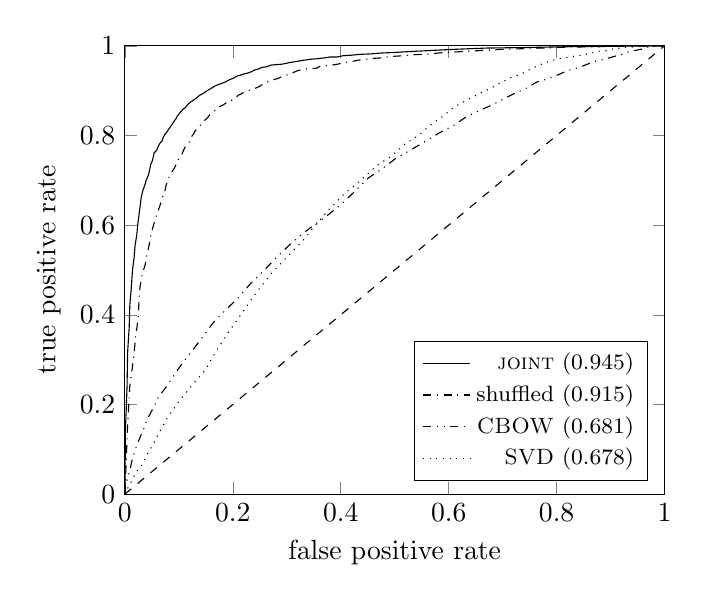
\begin{tikzpicture}
    \begin{axis}[xmin=0,xmax=1,ymin=0,ymax=1,xlabel={false positive rate},ylabel={true positive rate},legend pos=south east,legend cell align={right},legend style={font=\footnotesize}]
      \addplot [dashed,forget plot] coordinates{(0,0) (1,1)};
      \addplot [] coordinates{(0.0,0.0) (0.001,0.143) (0.004,0.240) (0.005,0.315) (0.008,0.373) (0.009,0.419) (0.012,0.463) (0.014,0.499) (0.017,0.527) (0.019,0.556) (0.022,0.578) (0.024,0.603) (0.026,0.621) (0.028,0.640) (0.030,0.660) (0.033,0.676) (0.037,0.690) (0.040,0.702) (0.044,0.713) (0.046,0.725) (0.048,0.736) (0.051,0.744) (0.053,0.754) (0.054,0.761) (0.059,0.767) (0.061,0.774) (0.065,0.783) (0.069,0.788) (0.071,0.796) (0.074,0.802) (0.078,0.808) (0.081,0.814) (0.084,0.819) (0.088,0.826) (0.092,0.833) (0.095,0.838) (0.097,0.843) (0.099,0.846) (0.102,0.851) (0.105,0.855) (0.108,0.859) (0.112,0.862) (0.116,0.868) (0.118,0.871) (0.121,0.874) (0.125,0.877) (0.128,0.880) (0.132,0.883) (0.136,0.887) (0.139,0.890) (0.144,0.893) (0.148,0.896) (0.151,0.899) (0.154,0.901) (0.157,0.903) (0.161,0.906) (0.165,0.909) (0.168,0.911) (0.174,0.914) (0.179,0.916) (0.183,0.918) (0.188,0.920) (0.190,0.922) (0.195,0.925) (0.200,0.927) (0.204,0.930) (0.209,0.933) (0.213,0.934) (0.220,0.937) (0.227,0.939) (0.234,0.942) (0.240,0.946) (0.247,0.948) (0.254,0.952) (0.262,0.953) (0.271,0.957) (0.280,0.958) (0.291,0.959) (0.299,0.961) (0.307,0.963) (0.318,0.965) (0.332,0.968) (0.345,0.970) (0.355,0.971) (0.369,0.973) (0.380,0.975) (0.393,0.975) (0.405,0.978) (0.419,0.979) (0.436,0.981) (0.456,0.982) (0.476,0.984) (0.497,0.985) (0.525,0.987) (0.558,0.989) (0.590,0.991) (0.627,0.993) (0.671,0.995) (0.732,0.996) (0.820,0.998) (1.0,1.0)}; %joint auc = 0.945
      \addplot [dash dot] coordinates{(0.0,0.0) (0.005,0.153) (0.009,0.240) (0.016,0.302) (0.020,0.352) (0.025,0.396) (0.026,0.430) (0.028,0.462) (0.032,0.489) (0.038,0.514) (0.041,0.534) (0.045,0.556) (0.048,0.576) (0.051,0.591) (0.055,0.609) (0.059,0.623) (0.063,0.637) (0.067,0.651) (0.070,0.663) (0.074,0.676) (0.076,0.687) (0.079,0.698) (0.082,0.708) (0.086,0.717) (0.090,0.724) (0.094,0.733) (0.096,0.742) (0.101,0.749) (0.106,0.759) (0.108,0.765) (0.111,0.773) (0.116,0.780) (0.119,0.785) (0.121,0.792) (0.124,0.798) (0.128,0.805) (0.130,0.810) (0.133,0.814) (0.136,0.818) (0.140,0.823) (0.144,0.828) (0.147,0.833) (0.151,0.837) (0.154,0.841) (0.157,0.846) (0.160,0.850) (0.163,0.853) (0.167,0.856) (0.169,0.860) (0.175,0.864) (0.176,0.865) (0.182,0.868) (0.188,0.873) (0.192,0.874) (0.197,0.878) (0.201,0.882) (0.204,0.884) (0.208,0.887) (0.210,0.890) (0.215,0.892) (0.218,0.895) (0.224,0.898) (0.231,0.901) (0.237,0.904) (0.243,0.906) (0.249,0.909) (0.255,0.914) (0.260,0.917) (0.265,0.920) (0.272,0.922) (0.277,0.925) (0.283,0.927) (0.291,0.931) (0.298,0.934) (0.306,0.937) (0.313,0.941) (0.321,0.945) (0.330,0.947) (0.340,0.949) (0.355,0.950) (0.361,0.954) (0.370,0.955) (0.383,0.957) (0.394,0.959) (0.408,0.963) (0.421,0.965) (0.432,0.968) (0.446,0.970) (0.460,0.972) (0.474,0.973) (0.492,0.976) (0.516,0.978) (0.535,0.980) (0.564,0.982) (0.591,0.985) (0.623,0.987) (0.653,0.989) (0.696,0.992) (0.749,0.994) (0.818,0.997) (1.0,1.0)}; %joint reshuffled auc = 0.915
      \addplot [dash dot dot] coordinates {(0.000,0.000) (0.000,0.001) (0.000,0.002) (0.001,0.006) (0.001,0.008) (0.001,0.012) (0.001,0.019) (0.002,0.025) (0.005,0.034) (0.008,0.047) (0.011,0.063) (0.014,0.079) (0.019,0.099) (0.025,0.118) (0.034,0.143) (0.041,0.166) (0.052,0.191) (0.062,0.216) (0.079,0.243) (0.092,0.267) (0.107,0.293) (0.123,0.317) (0.143,0.349) (0.164,0.383) (0.186,0.410) (0.210,0.438) (0.233,0.470) (0.257,0.498) (0.281,0.528) (0.305,0.556) (0.327,0.579) (0.355,0.604) (0.381,0.627) (0.406,0.652) (0.429,0.679) (0.451,0.705) (0.478,0.727) (0.501,0.748) (0.530,0.768) (0.557,0.787) (0.583,0.806) (0.610,0.823) (0.633,0.842) (0.656,0.855) (0.682,0.869) (0.701,0.881) (0.724,0.895) (0.745,0.906) (0.763,0.919) (0.783,0.926) (0.804,0.936) (0.821,0.945) (0.840,0.951) (0.857,0.959) (0.870,0.965) (0.885,0.969) (0.897,0.973) (0.909,0.977) (0.920,0.980) (0.929,0.985) (0.943,0.989) (0.951,0.991) (0.960,0.993) (0.966,0.996) (0.973,0.998) (0.977,0.999) (0.983,0.999) (0.987,0.999) (0.991,1.000) (0.995,1.000) (0.998,1.000) (0.999,1.000) (1.000,1.000)}; %cbow, auc = 0.681
      \addplot [dotted] coordinates{(0.000,0.000) (0.000,0.001) (0.001,0.002) (0.001,0.003) (0.002,0.004) (0.003,0.007) (0.004,0.011) (0.007,0.016) (0.009,0.022) (0.013,0.030) (0.017,0.040) (0.024,0.055) (0.033,0.067) (0.040,0.087) (0.051,0.108) (0.063,0.136) (0.079,0.171) (0.101,0.208) (0.123,0.241) (0.149,0.277) (0.169,0.319) (0.192,0.361) (0.216,0.402) (0.240,0.444) (0.269,0.489) (0.298,0.526) (0.331,0.567) (0.353,0.600) (0.378,0.635) (0.406,0.669) (0.437,0.700) (0.466,0.732) (0.496,0.756) (0.519,0.781) (0.545,0.801) (0.566,0.823) (0.587,0.841) (0.611,0.864) (0.634,0.879) (0.654,0.892) (0.676,0.904) (0.697,0.918) (0.715,0.929) (0.736,0.938) (0.753,0.949) (0.772,0.959) (0.786,0.965) (0.802,0.971) (0.818,0.974) (0.834,0.977) (0.851,0.980) (0.863,0.984) (0.878,0.988) (0.891,0.989) (0.899,0.992) (0.909,0.994) (0.920,0.995) (0.928,0.996) (0.936,0.997) (0.945,0.998) (0.950,0.999) (0.956,0.999) (0.963,0.999) (0.967,1.000) (0.972,1.000) (0.978,1.000) (0.983,1.000) (0.989,1.000) (0.994,1.000) (0.996,1.000) (0.997,1.000) (0.999,1.000) (1.000,1.000)}; %svd 2x50, auc = 0.678
      \legend{\textsc{joint} (0.945),shuffled (0.915),\textsc{CBOW} (0.681),\textsc{SVD} (0.678)} 
    \end{axis}
  \end{tikzpicture}
\caption[Receiver Operating Characterisation for Metaphor Classification]{Receiver operating characteristic plots for a selection of models, with the area under the curve for each model type indicated in the legend.}
\label{fig:metaroc}
\end{figure}

With the trade off between true and false positives in mind, Table~\ref{tab:metastats} presents precision, recall, f-score, accuracy, and Cohen's kappa scores for the same models plotted in Figure~\ref{fig:metaroc}, along with a majority class baseline and the scores originally achieved by \cite{GutierrezEA2016}.  The trend to notice here is that context sensitive and static models tend to favour recall over precision (and the slight preference for precision in the \textsc{joint} 400 dimensional, 5x5 word subspaces for the shuffled version of the data reported here is an anomaly, as other approaches to that data exhibit the tendency towards higher recall).  This evident enthusiasm for classifying phrases as metaphoric is a reflection of the data itself, which is slightly skewed towards metaphoric phrases, as described above and indicated in the performance of the majority class baseline, and this is reinforced by the relatively low accuracy scores for both context sensitive and static non-compositional distributional semantic models.  It is noteworthy, then, that the model described by \cite{GutierrezEA2016} actually scores better for precision than recall, suggesting it tends to under-predict metaphoricity.  This could perhaps be expected as a general distinction between statistical models based on unannotated data such as mine, which will arguably tend to favour a majority class, versus likewise statistical models operating on theoretically motivated mappings between representations, which have an apparent propensity for zeroing in with confidence on the properties of a compositional transformation that are indicative of metaphor---but at the expense of sometimes missing what might be considered outliers.  In the same spirit, the jumpier nature of the receiver operating characteristic plots presented by \cite{TsvetkovEA2014} is quite possibly an artefact of the decision points inherent in heuristically mapping model features from human made knowledge bases.

\begin{table}
\centering
\begin{tabular}{lrrrrr}
\hline
\ & \emph{precision} & \emph{recall} & \emph{f-score} & \emph{accuracy} & \emph{kappa} \\
\hline
\textsc{joint} & 0.879 & 0.894 & 0.886 & 0.877 & 0.753\\
shuffled & 0.873 & 0.865 & 0.862 & 0.854 & 0.678 \\
\textsc{SVD} & 0.631 & 0.794 & 0.703 & 0.641 & 0.265 \\
\textsc{CBOW} & 0.638 & 0.721 & 0.677 & 0.632 & 0.253 \\
\cite{GutierrezEA2016} & 0.842 & 0.793 & 0.817 & 0.809 & 0.618 \\
baseline & 0.535 & 1.000 & 0.697 & 0.535 & 0.000 \\
\hline
\end{tabular}
\caption[Comparative Metaphor Classification Statistics]{Full classification statistics results for the models tested here as well as the results from the original literature and the majority class (metaphor) baseline.}
\label{tab:metastats}
\end{table}

As a final point of comparison with other approaches to metaphor classification, I will return briefly to the unannotated character of my lexical representations.  One of the most powerful features of the methodology described here is its ability to build a somewhat general model of a semantic phenomenon from a sufficiently comprehensive dataset, and the strong Cohen's kappa score of the best performing subspace selection technique, which begins to approach the aforementioned inter-annotator agreement level of $\kappa = 0.80$, is a testament to this.  \revJB{33}{This statistic measure inter-annotator agreement that it offsets the accuracy $a$ inherent in the overlap between annotators with the hypothetical probability of annotators agreeing by chance} \citep{Cohen1960}:

\begin{equation}
\revJB{33}{\kappa = \frac{a-p}{1-p}}
\end{equation}

\noindent\revJB{33}{As such, this becomes a more stringent measure as the correlation between two sets of classifications approaches perfect accuracy.}  Following an analysis of the specific geometry of metaphor in the next section, Section~\ref{sec:genaphor} will assess the ability of my methodology to generalise even further from this data to a broader range of metaphors and to moreover move from classification to gradation based on observations of merely binary judgements of metaphoricity.  For now, I simply note that it is remarkable that data about nothing more than the way that words tend to be collocated can, with the aid of a mechanism for contextualisation, reveal so much about the nature of the semantic relationship between the lexical components of a previously unseen phrase.

\subsection{The Geometry of Metaphor}
In this section, I will explore the geometric features which prove most productive in the classification of metaphor.  As with relatedness and similarity in the previous chapter, I begin by examining the capacity of independent features to predict metaphor.  Rather than a proper logistic regression involving multiple independent variables fed into a non-linear function, this analysis amounts to choosing a cut-off point in terms of the value of each feature separating literal and metaphoric phrases in the subspaces which an analysis of their corresponding word-vectors delineate.  So the f-scores reported in Table~\ref{tab:ind-metaphor} can be understood as indicating the degree to which the values of a given geometric feature separate the dataset into distinct categories corresponding to human judgements of metaphoricity.

\begin{table}
\centering
\begin{tabular}{lr|lr|lr}
\hline
\multicolumn{2}{c}{\textsc{joint}} & \multicolumn{2}{c}{\textsc{indy}} & \multicolumn{2}{c}{\textsc{zipped}} \\
\hline
$\mu(A,B)$ & 0.787 & $C$ & 0.767 & $\mu(A,B)$ & 0.788 \\
$C$ & 0.771 & $C/M$ & 0.749 & $C$ & 0.771 \\
$\mu(A,B)/M$ & 0.764 & $\angle AMB$ & 0.747 & $\mu(A,B)/M$ & 0.769 \\
$\angle COX$ & 0.762 & $C/X$ & 0.746 & $X$ & 0.767 \\
$X$ & 0.762 & $\mu(A,B)$ & 0.734 & $\mu(A,B)/X$ & 0.759 \\
\hline
\end{tabular}
\vfill
\begin{tabular}{lr|lr}
\multicolumn{2}{c}{\textsc{adjective}} & \multicolumn{2}{c}{\textsc{noun}} \\
\hline
$\mu(A,B)/M$ & 0.745 & $\mu(A,B)$ & 0.756 \\
$\overline{AC}:\overline{BC}$ & 0.736 & $C$ & 0.747 \\
$\overline{AC}/\overline{BC}$ & 0.734 & $\mu(A,B)/X$ & 0.728 \\
$\mu(A,B)/X$ & 0.732 & $\mu(A,B)/M$ & 0.721 \\
$\angle ACB$ & 0.730 & $C/X$ & 0.721 \\
\hline
\end{tabular}
\caption[Top Independent Features for Metaphor Classification]{Independent f-scores from the metaphor classification data for top five features of each subspace type for 5x5 word co-occurrence window, 400 dimension subspaces.}
\label{tab:ind-metaphor}
\end{table}

%\begin{table}
%\centering
%\begin{tabular}{lr|lr|lr|lr|lr}
%\hline
%\multicolumn{2}{c}{\textsc{joint}} & \multicolumn{2}{c}{\textsc{indy}} & \multicolumn{2}{c}{\textsc{zipped}} & \multicolumn{2}{c}{\textsc{adjective}} & \multicolumn{2}{c}{\textsc{noun}} \\
%\hline
%$\mu(A,B)$ & 0.785 & $C$ & 0.767 & $\mu(A,B)$ & 0.788 & $\mu(A,B)/M$ & 0.744 & $\mu(A,B)$ & 0.756 \\
%$C$ & 0.768 & $\angle AMB$ & 0.749 & $\mu(A,B)/M$ & 0.771 & $\overline{AC}:\overline{BC}$ & 0.737 & $C$ & 0.745 \\
%$\mu(A,B)/M$ & 0.764 & $C/M$ & 0.748 & $X$ & 0.769 & $\mu(A,B)/C$ & 0.736 & $\mu(A,B)/X$ & 0.728 \\
%$X$ & 0.763 & $C/X$ & 0.747 & $C$ & 0.767 & $\mu(A,B)/X$ & 0.733 & $\mu(A,B)/M$ & 0.722 \\
%$\mu(A,B)/X$ & 0.759 & $\mu(A,B)$ & 0.733 & $\mu(A,B)/X$ & 0.762 & $\angle ACB$ & 0.732 & $C/X$ & 0.721 \\
%\hline
%\end{tabular}
%\caption[Top Independent Features for Metaphor Classification with Unseen Adjectives]{Independent f-scores from the metaphor classification data for top five features of each subspace type for 5x5 word co-occurrence window, 400 dimension subspaces with models tested on adjectives not observed in training.}
%\label{tab:ind-metaphor}
%\end{table}

The scores themselves reflect the trend observed in Table~\ref{tab:metaphor} and~\ref{tab:categoraphor}: the \textsc{joint} and \textsc{zipped} subspaces produce features that are particulary good at classifying metaphor, with a decrease in performance in the \textsc{indy} subspaces and then another step down in the single-word subspaces.  None of the scores themselves come close to the levels of discrimination achieved by the models learned from full feature vectors, with the difference between the performance of the best feature for the \textsc{joint} technique and that of the corresponding full featured space somehwat significant at $p = .006$.  In terms of the actual features indicated by this analysis, two in particular figure prominently in one way or another, namely, the mean of the word-vector norms $\mu(A,B)$ and the norm of the central-vector $C$.  In the first instance, the role of the relationship between word-vectors and the origin of the spaces that their salient co-occurrence dimensions delineate is once again reflective of the preliminary findings on conceptual geometry described in Chapter~\ref{sec:poc}, where norm was seen to be an effective mechanism for defining a region of conceptual constituency.  In the case of the distance of the central vector from the origin, the emergence of this feature, as well of the appearance of the norms $M$ and $X$ as components of various strongly predictive tendencies, indicate that here, as with similarity in the previous chapter, characteristics of dimensions outside of the situation of any particular word-vector along them might be in themselves indicative of metaphor: some words might simply be more likely to co-occur in the context of metaphoric language, and a trend in the mean or maximum values of those words' co-occurrence profiles might provide a handle for examining this tendency.

To further delve into the statistical geometry of metaphor, and in line with the results on relatedness and similarity described in the previous chapter, I once again search the state space of possible combinations of features to find the optimal feature vector for classifying metaphor in context sensitive subspaces.  This is again treated as a beam search problem, though the search space expanded at each level of the search tree is here limited to the top 500 combinations of features given the larger size of the data being modelled.  Table~\ref{tab:metatures} presents the optimal seven feature combinations discovered for the 5x5 word window, 400 dimensional \textsc{joint} subspaces based on both a standard ten-fold cross-validation and the version of the data shuffled in order to test on adjectives not observed in each training phase.  The f-scores achieved by these combinations of features, reported next to the respective labels at the top of the table, indicate a marginal decrease in the overall performance as compared to the full featured models of subspaces, but the results are still strong.

\begin{table}
\centering
\begin{tabular}{llr}
\hline
& \multicolumn{1}{c}{10-fold ($f = 0.869$)} & \multicolumn{1}{c}{shuffled ($f = 0.830$)} \\
\hline
& \multicolumn{2}{c}{\textsc{distances}} \\
word-vectors& - & - \\
generic vectors & $M = -1.448$ & - \\
\hline
& \multicolumn{2}{c}{\textsc{angles}} \\
word-vectors & $\angle ACB = -0.775$ & - \\
normalised & - & - \\
generic vectors & $\angle COX = -1.618$ & $-0.271 = \angle COM$  \\
& $\angle COM = 0.974$ & $0.045 = \angle MOX$ \\
\hline
& \multicolumn{2}{c}{\textsc{means}} \\
word-vectors & $\mu(\overline{AM},\overline{BM}) = -1.124$ & $-1.007 = \mu(\overline{AC},\overline{BC})$ \\
normalised & - & - \\
\hline
& \multicolumn{2}{c}{\textsc{ratios}} \\
word-vectors & - & $0.492 = \overline{AM}:\overline{BM}$ \\
& & $-0.620 = \overline{AX}:\overline{BX}$ \\
normalised & - & $-0.168 = \overline{A'C'}:\overline{B'C'}$ \\
\hline
& \multicolumn{2}{c}{\textsc{fractions}} \\
word-vectors & $\overline{AC}/\overline{BC} = 0.325$ & - \\
generic vectors & $M/X = 1.305$ & $0.252 = A/B$ \\
\hline
\end{tabular}
\caption[Most Predictive Feature Vectors for Metaphor Classification]{The seven most predictive features for metaphor classification, compared between ten-fold and sight-unseen cross-validation of logistic regression on statistics extrapolated from 5x5 word window, 400 dimensional \textsc{joint} subspaces.}
\label{tab:metatures}
\end{table}

Angles between generic vectors, which were already evident as independently predictive features in Table~\ref{tab:ind-metaphor}, have a strong effect here, with the strong negative correlation of $\angle COX$ in the ten-fold cross-validation in particular suggesting that maximal values tend to be relatively similar across dimensions jointly selected by literal adjective-noun combinations, pulling the line of $X$ closer to the centroid described by $C$.  To put this differently, as pairs become more metaphoric, they tend to also become less consistent in the type of dimension that they co-select, as evidenced in the increasing variance in the maximum values of these dimensions.  Perhaps the most interesting thing to observe here, though, is the strong correlation between ratios of word-vector to generic vector distances in the case of the version of the data shuffled to test on unseen adjectives, but not in the case of the stratified cross-validation.  The positive correlation with the balance of the distances from the word-vectors to the mean vector $M$ means that subspaces where the word-vectors have a relatively even relationship to the weighted centre are, in fact, more metaphoric (and their relationship to the maximum vector is comparatively less balanced, with this vector in turn being less central to the space per the observations regarding $\angle COX$).  But more generally, it is noteworthy that the balance between word vectors and generic vectors is informative about metaphoricity specifically in models tested on unseen adjectives: this balance is in effect a projection into space of the ratio of set of propositions about the individual ratios of the conditional probability of a dimension being a co-occurrence term for a word compared to the mean conditional probability of that same dimension being a co-occurrence term for any word.

Figure~\ref{fig:metaspaces} presents visualisations by way of three dimensional projections of word-vectors and generic vectors from 400 dimensional \textsc{joint} subspaces selected from the 5x5 word window base space.\footnote{These projections have been rendered using the same regression technique as applied to the images for related word pairs in the previous section, but the coordinates of $X$ have been divided by 1.5 instead of 2.}  \revAK{2}{These examples have been chosen because they are at the high, middle, and low points of the distribution of scores output by this model, and also because they seem categorically exemplary of different degrees of metaphoricity.}  In the example of the uncontroversially literal phrase \emph{sweet watermelon}, the word-vectors are characteristically far from the origin and close to one another, corresponding to the predictivity of $\mu(A,B)$ in particular.  At the other extent of the spectrum, the highly metaphoric phrase \emph{bitter letter} is characterised by a dropping of the word-vectors and a widening of the angle between them; the generic vectors, meanwhile, are now further from the origin relative to the word-vectors that select the subspace and, at the same time, draw closer to one another in particular at the normalised layer of the subspace.  But most interestingly, at a relatively neutral point, occupied by the intriguingly ambiguous phrase \emph{warm country}, which the logistic regression trained on these subspaces assigned a score close to 0.5, there is actually evidence of an intermediary widening out of the overall array of points \del{even as the word-vectors remain fairly far from the origin} \revJB{34}{preceding the contraction of overall geometry in the literal case}.

\begin{figure}
\footnotesize
\begin{subfigure}{0.3\textwidth} % sour - sauce
\centering
  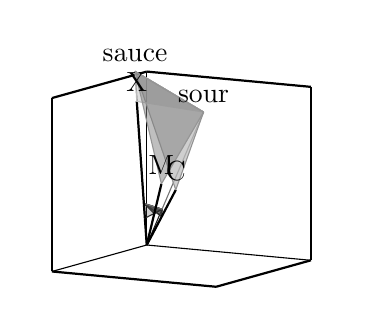
\begin{tikzpicture}
    \def\varA{(56.2720,60.1719,75.2389)};
    \def\varB{(73.7099,36.8692,94.6119)};
    \def\varC{(33.4740,33.4737,33.4739)};
    \def\varM{(36.1929,28.0423,36.1855)};
    \def\varX{(117.9619,63.2478,89.8183)};
    \def\varAN{(15.1308,16.1795,20.2308)};
    \def\varBN{(17.6235,8.8151,22.6210)};
    \def\varCN{(17.3206,17.3204,17.3205)};
    \def\varMN{(18.6056,14.4156,18.6017)};
    \def\varXN{(21.9544,11.7713,16.7165)};
    \def\nodA{56.2720,60.1719,75.2389};
    \def\nodB{73.7099,36.8692,94.6119};
    \def\nodC{33.4740,33.4737,33.4739};
    \def\nodM{36.1929,28.0423,36.1855};
    \def\nodX{117.9619,63.2478,89.8183};
    \begin{axis}[scale = 0.6,axis line style=white,view={120}{10},xmin=0,xmax=100,ymin=0,ymax=100,zmin=0,zmax=100,colormap/blackwhite,ticks=none]
      \addplot3[color=black,thick] coordinates {(0,0,80) (0,80,80)};
      \addplot3[color=black,thick] coordinates {(0,0,80) (80,0,80)};
      \addplot3[color=black,thick] coordinates {(0,80,0) (0,80,80)};
      \addplot3[color=black,thick] coordinates {(0,80,0) (80,80,0)};
      \addplot3[color=black,thick] coordinates {(80,0,0) (80,0,80)};
      \addplot3[color=black,thick] coordinates {(80,0,0) (80,80,0)};
      \addplot3[color=black] coordinates {(0,0,0) (0,0,80)};
      \addplot3[color=black] coordinates {(0,0,0) (0,80,0)};
      \addplot3[color=black] coordinates {(0,0,0) (80,0,0)};
      \addplot3[patch,patch type=triangle,color=gray,fill opacity=0.0] coordinates {(0.0,0.0,0.0) \varCN \varAN};
      \addplot3[patch,patch type=triangle,color=gray,fill opacity=0.0] coordinates {(0.0,0.0,0.0) \varCN \varBN};
      \addplot3[patch,patch type=triangle,color=darkgray,fill opacity=0.75] coordinates {\varCN \varAN \varBN};
      \addplot3[patch,patch type=triangle,color=darkgray,fill opacity=0.5] coordinates {\varMN \varAN \varBN};
      \addplot3[patch,patch type=triangle,color=darkgray,fill opacity=0.25] coordinates {\varXN \varAN \varBN};
      \addplot3 [color=black,thick] coordinates {(0,0,0) \varCN};
      \addplot3 [color=black,thick] coordinates {(0,0,0) \varXN};
      \addplot3 [color=black,thick] coordinates {(0,0,0) \varMN};
%      \addplot3[opacity = 0.1,surf,z buffer = sort,samples = 21,variable = \u,variable y = \v,domain = 0:90,y domain = 0:90,]
%    ({1*cos(u)*sin(v)}, {1*sin(u)*sin(v)}, {1*cos(v)});
      \addplot3 [patch,patch type=rectangle,color=lightgray,fill opacity=0.0] coordinates{\varAN \varA \varB \varBN
};
      \addplot3 [color=black,thick] coordinates {\varCN \varC};
      \addplot3 [color=black,thick] coordinates {\varXN \varX};
      \addplot3 [color=black,thick] coordinates {\varMN \varM};
      \addplot3 [patch,patch type=triangle,color=lightgray,fill opacity=0.75] coordinates{\varA \varC \varB};
      \addplot3 [patch,patch type=triangle,color=gray,fill opacity=0.25] coordinates{\varA \varX \varB};
      \addplot3 [patch,patch type=triangle,color=gray,fill opacity=0.5] coordinates{\varA \varM \varB};
      \node [anchor=south] at (axis cs: \nodA) {sour};
      \node [anchor=south] at (axis cs: \nodB) {sauce};
      \node [anchor=south] at (axis cs: \nodC) {C};
      \node [anchor=south] at (axis cs: \nodX) {X};
      \node [anchor=south] at (axis cs: \nodM) {M};
    \end{axis}
  \end{tikzpicture}
\caption*{\footnotesize \emph{literal: sweet watermelon}}
\end{subfigure}
\hfill
\begin{subfigure}{0.3\textwidth} % warm - country
\centering
  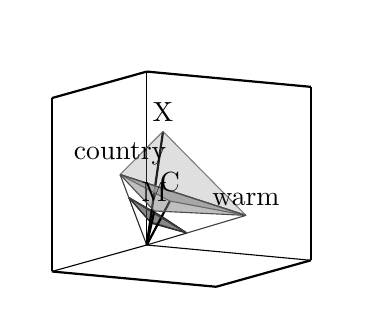
\begin{tikzpicture}
\def\varA{-8.639,51.611,50.881};
    \def\varA{(28.1002,64.5545,23.6443)};
    \def\varB{(25.5857,1.7784,36.5694)};
    \def\varC{(26.7296,26.7293,26.7296)};
    \def\varM{(33.9479,23.3011,22.9391)};
    \def\varX{(106.0249,69.1555,74.6834)};
    \def\varAN{(11.3507,26.0758,9.5508)};
    \def\varBN{(17.1844,1.1944,24.5615)};
    \def\varCN{(17.3206,17.3204,17.3206)};
    \def\varMN{(21.6073,14.8308,14.6004)};
    \def\varXN{(21.6416,14.1159,15.2442)};
    \def\nodA{28.1002,64.5545,23.6443};
    \def\nodB{25.5857,1.7784,36.5694};
    \def\nodC{26.7296,26.7293,26.7296};
    \def\nodM{33.9479,23.3011,22.9391};
    \def\nodX{106.0249,69.1555,74.6834};
    \begin{axis}[scale = 0.6,axis line style=white,view={120}{10},xmin=0,xmax=100,ymin=0,ymax=100,zmin=0,zmax=100,colormap/blackwhite,ticks=none]
      \addplot3[color=black,thick] coordinates {(0,0,80) (0,80,80)};
      \addplot3[color=black,thick] coordinates {(0,0,80) (80,0,80)};
      \addplot3[color=black,thick] coordinates {(0,80,0) (0,80,80)};
      \addplot3[color=black,thick] coordinates {(0,80,0) (80,80,0)};
      \addplot3[color=black,thick] coordinates {(80,0,0) (80,0,80)};
      \addplot3[color=black,thick] coordinates {(80,0,0) (80,80,0)};
      \addplot3[color=black] coordinates {(0,0,0) (0,0,80)};
      \addplot3[color=black] coordinates {(0,0,0) (0,80,0)};
      \addplot3[color=black] coordinates {(0,0,0) (80,0,0)};
      \addplot3[patch,patch type=triangle,color=gray,fill opacity=0.0] coordinates {(0.0,0.0,0.0) \varCN \varAN};
      \addplot3[patch,patch type=triangle,color=gray,fill opacity=0.0] coordinates {(0.0,0.0,0.0) \varCN \varBN};
      \addplot3[patch,patch type=triangle,color=darkgray,fill opacity=0.75] coordinates {\varCN \varAN \varBN};
      \addplot3[patch,patch type=triangle,color=darkgray,fill opacity=0.5] coordinates {\varMN \varAN \varBN};
      \addplot3[patch,patch type=triangle,color=darkgray,fill opacity=0.25] coordinates {\varXN \varAN \varBN};
      \addplot3 [color=black,thick] coordinates {(0,0,0) \varCN};
      \addplot3 [color=black,thick] coordinates {(0,0,0) \varXN};
      \addplot3 [color=black,thick] coordinates {(0,0,0) \varMN};
%      \addplot3[opacity = 0.1,surf,z buffer = sort,samples = 21,variable = \u,variable y = \v,domain = 0:90,y domain = 0:90,]
%    ({1*cos(u)*sin(v)}, {1*sin(u)*sin(v)}, {1*cos(v)});
      \addplot3 [patch,patch type=rectangle,color=lightgray,fill opacity=0.0] coordinates{\varAN \varA \varB \varBN
};
      \addplot3 [color=black,thick] coordinates {\varCN \varC};
      \addplot3 [color=black,thick] coordinates {\varXN \varX};
      \addplot3 [color=black,thick] coordinates {\varMN \varM};
      \addplot3 [patch,patch type=triangle,color=lightgray,fill opacity=0.75] coordinates{\varA \varC \varB};
      \addplot3 [patch,patch type=triangle,color=gray,fill opacity=0.25] coordinates{\varA \varX \varB};
      \addplot3 [patch,patch type=triangle,color=gray,fill opacity=0.5] coordinates{\varA \varM \varB};
      \node [anchor=south] at (axis cs: \nodA) {warm};
      \node [anchor=south] at (axis cs: \nodB) {country};
      \node [anchor=south] at (axis cs: \nodC) {C};
      \node [anchor=south] at (axis cs: \nodX) {X};
      \node [anchor=south] at (axis cs: \nodM) {M};
    \end{axis}
  \end{tikzpicture}
\caption*{\footnotesize \emph{neutral: warm country}}
\end{subfigure}
\hfill
\begin{subfigure}{0.3\textwidth} % bitter - letter
\centering
  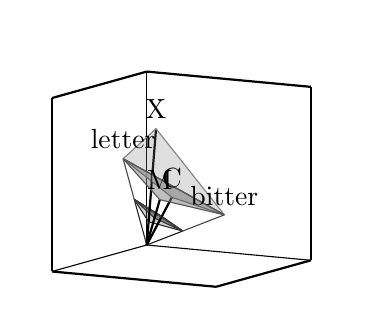
\begin{tikzpicture}
    \def\varA{(27.7652,53.8416,22.8974)};
    \def\varB{(33.0985,7.5929,45.5444)};
    \def\varC{(28.9808,28.9805,28.9808)};
    \def\varM{(33.1872,25.5252,28.2293)};
    \def\varX{(109.8650,67.9613,76.3988)};
    \def\varAN{(12.8618,24.9413,10.6069)};
    \def\varBN{(17.4783,4.0096,24.0506)};
    \def\varCN{(17.3206,17.3204,17.3206)};
    \def\varMN{(19.7168,15.1648,16.7713)};
    \def\varXN{(21.9604,13.5845,15.2710)};
    \def\nodA{27.7652,53.8416,22.8974};
    \def\nodB{33.0985,7.5929,45.5444};
    \def\nodC{28.9808,28.9805,28.9808};
    \def\nodM{33.1872,25.5252,28.2293};
    \def\nodX{109.8650,67.9613,76.3988};
    \begin{axis}[scale = 0.6,axis line style=white,view={120}{10},xmin=0,xmax=100,ymin=0,ymax=100,zmin=0,zmax=100,colormap/blackwhite,ticks=none]
      \addplot3[color=black,thick] coordinates {(0,0,80) (0,80,80)};
      \addplot3[color=black,thick] coordinates {(0,0,80) (80,0,80)};
      \addplot3[color=black,thick] coordinates {(0,80,0) (0,80,80)};
      \addplot3[color=black,thick] coordinates {(0,80,0) (80,80,0)};
      \addplot3[color=black,thick] coordinates {(80,0,0) (80,0,80)};
      \addplot3[color=black,thick] coordinates {(80,0,0) (80,80,0)};
      \addplot3[color=black] coordinates {(0,0,0) (0,0,80)};
      \addplot3[color=black] coordinates {(0,0,0) (0,80,0)};
      \addplot3[color=black] coordinates {(0,0,0) (80,0,0)};
      \addplot3[patch,patch type=triangle,color=gray,fill opacity=0.0] coordinates {(0.0,0.0,0.0) \varCN \varAN};
      \addplot3[patch,patch type=triangle,color=gray,fill opacity=0.0] coordinates {(0.0,0.0,0.0) \varCN \varBN};
      \addplot3[patch,patch type=triangle,color=darkgray,fill opacity=0.75] coordinates {\varCN \varAN \varBN};
      \addplot3[patch,patch type=triangle,color=darkgray,fill opacity=0.5] coordinates {\varMN \varAN \varBN};
      \addplot3[patch,patch type=triangle,color=darkgray,fill opacity=0.25] coordinates {\varXN \varAN \varBN};
      \addplot3 [color=black,thick] coordinates {(0,0,0) \varCN};
      \addplot3 [color=black,thick] coordinates {(0,0,0) \varXN};
      \addplot3 [color=black,thick] coordinates {(0,0,0) \varMN};
%      \addplot3[opacity = 0.1,surf,z buffer = sort,samples = 21,variable = \u,variable y = \v,domain = 0:90,y domain = 0:90,]
%    ({1*cos(u)*sin(v)}, {1*sin(u)*sin(v)}, {1*cos(v)});
      \addplot3 [patch,patch type=rectangle,color=lightgray,fill opacity=0.0] coordinates{\varAN \varA \varB \varBN
};
      \addplot3 [color=black,thick] coordinates {\varCN \varC};
      \addplot3 [color=black,thick] coordinates {\varXN \varX};
      \addplot3 [color=black,thick] coordinates {\varMN \varM};
      \addplot3 [patch,patch type=triangle,color=lightgray,fill opacity=0.75] coordinates{\varA \varC \varB};
      \addplot3 [patch,patch type=triangle,color=gray,fill opacity=0.25] coordinates{\varA \varX \varB};
      \addplot3 [patch,patch type=triangle,color=gray,fill opacity=0.5] coordinates{\varA \varM \varB};
      \node [anchor=south] at (axis cs: \nodA) {bitter};
      \node [anchor=south] at (axis cs: \nodB) {letter};
      \node [anchor=south] at (axis cs: \nodC) {C};
      \node [anchor=south] at (axis cs: \nodX) {X};
      \node [anchor=south] at (axis cs: \nodM) {M};
    \end{axis}
  \end{tikzpicture}
\caption*{\footnotesize \emph{metaphoric: bitter letter}}
\end{subfigure}
\caption[Metaphors In Space]{Three dimensional projections of word-vectors and generic vectors in subspaces for pairs at the extents and in the middle of the literal-metaphorical spectrum, taken from 5x5 word window, 400 dimensional subspaces selected using the \textsc{joint} technique.}
\label{fig:metaspaces}
\end{figure}

The exciting thing about this last observation is that it suggests that, rather than existing on a linear or even monotonic scale, metaphor may itself actually be a multi-dimensional phenomenon, with a characteristic particular to highly ambiguous word combinations that is to some extent separate from the statistical features of straightforward literalness and clear cut metaphoricity.  The broad arrangement of word-vectors in space engendered by the contextualisation of the phrase \emph{warm country}, in contrast to the relatively tight relationship of the generic vectors, can be interpreted as revealing an uncertainty regarding the semantic properties being transferred in this small composition, corresponding to a drifting of the word-vectors and a contracting of the generic vectors across the jointly selected co-occurrence profile.  Here, once again, the statistical geometry of a subspace can be productively mapped to a theoretical statement about the nature of a semantic phenomenon as characterised by a selectively contextual and quantitative representation of observations about the way that words are used, by and large outside of any strong preconditions symbolically encoded in the computational framework.

\subsection{Generalising the Model} \label{sec:genaphor}
One of the interesting things about feature-based classification is that there is typically an inherent commitment to degree of class membership, even when the training data used to build a model is simply binary.  This is true of any model which uses, for instance, a logistic regression technique for determining class, as there is a cut-off point along the spectrum of model output and a corresponding proximity to that point for any given sample, and it is especially obvious when the features of the model are actually geometrical measures.  In this section, I will apply the models learned from the the \cite{GutierrezEA2016} data to another dataset designed to assess metaphor as a matter of degree rather than simply as a binary situation, and a dataset that additionally deals with a different type of metaphor in terms of composition.  The question explored here is whether the geometric features of context specific distributional semantic analysis of word-vectors will provide binary classification models with adequate information for projecting metaphoricity along a continuous scale.

The data used for this experiment was originally reported by \cite{JankowiakEA2015}, and was used to train a model based on an earlier version of my methodology as described by \cite{AgresEA2016}.  This data consists of 228 predicate-object word pairs selected to cover three degrees of metaphor, consisting of literal pairs such as \emph{announce willingness}, conventionally metaphoric pairs such as \emph{cut pollution}, and novel metaphors such as \emph{smell excuses}.  102 human participants provided metaphoricity scores on a seven point Likert scale, and the average scores were compiled into the dataset that will used to test models learned from the geometric features output by my context sensitive methodology.\footnote{Studies were also conducted to gather ratings for \emph{familiarity} and \emph{meaningfulness}, but those ratings will not be modelled in this thesis.}  Specifically, I will experiment with two different classification model techniques.  In the first instance, I will take the output of the logistic regression described above, trained on the \cite{GutierrezEA2016} data, as assigning probabilities to the metaphoricity of an input word pair, and I will in turn measure the degree to which these probabilities correlate with the degree of metaphoricity collectively assigned by human raters.  In the second instance, I'll use the binary metaphor classification data to train a support vector machine.\footnote{This is implemented using the python scikit-learn \texttt{SVC} module.}  Applying a radial basis function kernel, I analyse the correlation between distance from the discriminatory hyperplane and the human ratings.  In both cases, and in line with results reported in the previous chapter, Spearman's correlations are the unit of analysis.

\begin{table}
\centering
\begin{tabular}{lrrrrrr}
\hline
\emph{features} & 1 & 3 & 5 & 7 & 9 & full \\
\hline
& \multicolumn{6}{c}{\emph{logistic regression}} \\
\textsc{joint} & 0.368 & 0.355 & 0.033 & 0.085 & 0.279 & -0.033 \\
\textsc{adjective} & -0.377 & 0.355 & 0.044 & 0.513 & 0.511 & 0.335 \\
\hline
& \multicolumn{6}{c}{\emph{support vector machine}} \\
\textsc{joint} & 0.352 & 0.359 & 0.042 & 0.045 & 0.243 & 0.158 \\
\textsc{adjective} & -0.170 & 0.247 & -0.021 & 0.407 & 0.418 & 0.236 \\
\hline
\end{tabular}
\caption[Scoring Metaphoricity Based On Classification Data]{Spearman's correlation with human verb-noun metaphoricity scales judgements based on logistic regression and support vector machine models trained on adjective-noun classification data, taking feature vectors of various lengths as independent variables.}
\label{tab:verblearn}
\end{table}

Table~\ref{tab:verblearn} presents results for both modelling techniques, focusing on features extrapolated from 5x5 word window, 400 dimensional subspaces using both the \textsc{joint} approach and an analysis of just the adjective in each word-pair from the input data.  Feature vectors of various lengths, picking the optimal geometric features for each dimensional selection technique, are used to feed input to each model.  In terms of the models trained on features from \textsc{joint} subspaces, there is a clear trend towards strong performance with one or three features, weaker performance with five or seven features, stronger performance again with nine features, and then a drop-off again in the full featured space.  The relatively low performance with the full set of features is not particularly surprising: there is clearly an encroaching incidence of generalisation error here as the models become flooded with data about various and certainly collinear statistical features of contextual geometry.  At the shallow end of the feature selection parameters, on the other hand, the single measure $\mu(A,B)$ (per Table~\ref{tab:ind-metaphor}) once again points to the efficacy of word-vector norm as a predictive characteristic of contextualised co-occurrence subspaces.

The really remarkable outcome here, though, is the very strong performance of the models learned from the top seven and nine features extracted from subspaces selected by PMI values of the adjective word-vectors alone.  This is particularly interesting given that the data being tested actually consists of a different type of grammatical relationship, namely, predicate-object pairs.  It would seem, then, that the co-occurrence dimensions most salient to either verbs or adjectives generate a geometry in which their relationship to potential arguments can play out in similar ways in terms of the graded metaphoricity inherent in the semantic context: the interaction between the selecting vector, the noun-vector, and the generic vectors translates from one type of composition to another in an isomorphic way.  This explantion, including the claim that the mapping of predictive features from one type of metaphor to the other is to a large extent isomorphic, is supported by the particularly strong performance of the logistic regression at seven and nine dimensions, where the logistic function takes a polynomial with coefficients learned in the training phase as direct input.  The more complex non-linearity afforded by the support vector machine appears to actually somewhat confound the mapping from verb-noun to adjective-noun phrases---though the difference between the correlations at nine dimensions is not statistically significant at $p = .104$ based on a Fisher r-to-z transformation.

The one area where a support vector machine provides a clear improvement in performance is in the full dimensional models extrapolated from \textsc{joint} subspaces.  In this case, it would seem that the radial basis function classification actually does a better job of avoiding the overfitting in a higher dimensional feature space.  But, putting questions of model choice aside, there is clear evidence here for the generality of the contextual geometry of metaphor, and also a strong case for the appropriateness of machine learning techniques for providing a mechanism for the computational manipulation of co-occurrence information to build a more nuanced model of degree of metaphor based on relatively rudimentary classification data.  Crucially, it is the context sensitivity of my methodology that facilitates the exploration of a multi-dimensional feature space in which the non-linear nuances of this particular semantic phenomenon can be discovered; a model providing a singular static relationship between lexical representations could not offer the context specific underpinning for generating a geometry replete with interpretable statistical features.  Finally, there are signs here to invite further research, and indeed some grounds for hoping that a context sensitive approach might have the scope for handling more sophisticated tasks such as metaphor interpretation and generation.

\section{An Experiment on Coercion} \label{sec:coerperiment}
In this section, I will apply my methodology to the classification of a phenomenon closely related to metaphor, namely, \emph{semantic type coercion}, by which the semantic type of a word is shifted through its interaction with another word: in the cases examined here, verbs that select for a particular semantic type will be seen to coerce nouns from one conceptual category to another by taking those nouns as arguments.  So, for instance, in phrases like \emph{denied wrongdoing} or \emph{heard footsteps}, the nouns in play are standing in for a conceptually relevant but different type of noun, and the literal versions of these phrases would go something like \emph{denied committing wrongdoing} or \emph{heard the sound of footsteps}, where the verbs select arguments of types along the lines of \textsc{activity} and \textsc{perception} respectively.  This phenomenon is often referred to as \emph{logical metonymy}, identifying it as a subspecies of the more general figurative phenomenon metonymy by which a thing is denoted by a conceptually related lexical representation.

\subsection{Background}
Coercion is one of the semantic phenomena targeted by \citepos{Pustejovsky1995} theory of a \emph{generative lexicon}, by which nouns are semantically modelled as having a \emph{qualia structure} which maps out the way that a thing relates to itself, the world, and the agents interacting with it in that world on four different levels of abstraction, with the general objective of arriving at ``a model of meaning in language that captures the means by which words can assume a potentially infinite number of senses in context, while limiting the number of senses actually stored in the lexicon,'' (p. 104).  In terms of coercion, qualia provide the basis for a process of \emph{projection} by which a variety of semantic types can be extracted from a complex type (or a \emph{dot object} in Pustejovsky's lingo) in order to fulfil the typing requirements of a predicate in open ended ways.  The model that emerges here -- one built on dynamically interactive lexical semantic representations contingent on some sort of general conceptual context -- begins to look like the general linguistic stance that has motivated my own methodology.

This theoretical commitment suggests a schematic by which a symbol manipulating system might begin to get a handle on productive and context sensitive lexical representations of things in the world.  To this end, \cite{JezekEA2010} have described an ontology based on a computational analysis of co-occurrence patterns designed to facilitate the modelling of what is ultimately a sliding scale of statistically enhanced semantic representations, or ``shimmering lexical sets,'' (p. 19), as the authors put it.  Applying a similar notion that coercion is probabilistic rather than discrete, \cite{LapataEA2003} use co-occurrence statistics to try to predict the verbs which, in the role of for instance participles, successfully resolve instances of coercion.  And, under the rubric of \emph{logical metonymy}, \cite{ShutovaEA2013b} expand upon the work of \citeauthor{LapataEA2003} by extracting verb senses from WordNet to build a class based model, to some extent recapitulating the categorical distinctions that characterise many theoretical approaches to coercion.  The motivation behind this last system is the apt observation that, in the case of coercion, ``humans are capable of interpreting these phrases using their world knowledge and contextual information,'' \citep[][11:2]{ShutovaEA2013b}.

Returning to the theoretical issues regarding grammaticality raised earlier in this chapter, the analysis of coercion within the framework of the generative lexicon points to something more like a graduated typology, sliding from specific instances of processes, things, and the like to more general conceptual categories and finally to entire classes of words.  As \cite{Langacker1991} has pointed out, there is a lurking ambiguity in grammatical class distinctions, with various conceptual schema existing in any natural language for moving between classes: so, to borrow an example from Langacker, phonological and symbolic dynamics facilitate a conceptually coherent progression from \emph{sharp} to \emph{sharpen} to \emph{sharpener}, and the rules that are extrapolated as an explanatory framework for such transitions are just a way of systematising the cognitive networks that underpin this linguistic phenotype.\footnote{\citepos{Wittgenstein1953} quip regarding ``grammatical fictions,'' (ibid, \P 307) also seems pertinent.}  And as \cite{CopestakeEA1995} point out in their probabilistic account of coercion, selectional preferences are at least to a certain extent conditioned by factors involving word frequency, suggesting that there could be grounds for a distributional mechanism for modelling semantic shifting.

With this in mind, my hypothesis is that, as with metaphor in the previous section, a syntactically neutral statistical model with a context generating capacity should be able to capture the way in which, in the case of argument type coercion, a predicate specifies some conceptual contingency of the coerced object in order to accommodate its selectional preference.  The purpose of this set of experiments \citep[an early version of which is reported in][]{McGregorEA2017} is to test this broad hypothesis, and to explore the particular statistical features of co-occurrence which afford appropriate contextualisations.  This will serve, to a certain extent, to address a question raised by \cite{PustejovskyEA2008}, who illustrate some of the difficulties inherent in extracting typological structure from a distributional analysis of a large-scale corpus.  The point made there is that ``generative mechanisms in the semantics, such as coercion, modulate meanings in context and allow words to behave distributionally in unexpected ways with respect to their selectional properties,'' (ibid, p. 209).  Those authors show how a model involving a dynamic between a statistical approach such as a distributional semantic model and a theoretical structure such as the generative lexicon can accommodate some of this unexpectedness.  My goal in the following experiments is to explore the extent to which a context sensitive approach to distributional semantics can, without the structure of a symbolic formalism or pre-formulated grammatical or typological annotations, address the pertinent theoretical issues raised by the kind of analysis offered by \citeauthor{PustejovskyEA2008}.

\subsection{Methodology and Results}
The data which will be used to test my methodology in this section was originally presented by \cite{PustejovskyEA2010} as a task for the ongoing International Workshop on Semantic Evaluation series of computational semantic modelling challenges.  The data consists of 2,071 sentences (originally split into a test set of 1,039 training instances and 1,032 testing instances)\footnote{The data is available under task seven at \url{http://semeval2.fbk.eu/semeval2.php?location=data}.} each containing a marked verb and object, with the object classified as either coercive or not.  \revAK{21}{Five verbs, each selecting for a different semantic type as an argument, were selected based on the basis of their tendency for coercion, as observed in sentences in the BNC, a balanced corpus of written and spoken British English, and the sentences comprising the data were likewise randomly drawn from this coprus.}  \del{The verbs cover various conjugations of five different verb stems, each identified as selecting for a different semantic type as an argument:} The verbs (and the semantic type selected) are \emph{arrive} (\textsc{location}), \emph{cancel} (\textsc{event}), \emph{deny} (\textsc{proposition}), \emph{finish} (\textsc{event}), and \emph{hear} (\textsc{sound}).  The objective, then, is to train a model to indicate that the phrase \emph{finish the party} is not coercive, in as much as we accept that \emph{party} denotes a member of the conceptual category \textsc{event}, whereas \emph{finish the food} is because what is actually being finished is the event of eating food, not the food itself.  For the purposes of the original presentation the data is split into a training set and a testing set of roughly equal size, but questions of the most meaningful partitioning of the data will be discussed below.

Two amendments are made to the data as presented.  First, of the 2,071 verb-object pairs, 78 contain multi-word objects not compatible with the vocabulary used for my model, reducing the total number of word pairs to 1,992, 591 of which are considered coercive.  Second, of these remaining computable word pairs, 903 are duplicates (they are presented in unique sentences, but for the first phase of analysis here only verb-noun pairs will be consider; sentential context will be addressed below).  This leaves a total of 1,029 word pairs, 399 of which are deemed coercive.  As with the metaphor data in the previous section, I train a logistic regression model to discriminate between regular argument selection and coercion.  I once again take the two words being analysed as input to generate a number of different context specific distributional semantic subspaces, treating the 34 geometric features outlined in Table~\ref{tab:features} plus the seven additional fractional features specific to asymmetric input terms described above in Section~\ref{sec:metameth} as the independent variables of the regression analysis.  \revAK{1}{As with results on metaphor classification, models with f-scores with $p < .01$ of being observed by chance based on a permutation test will be considered statistically significant.}

%\begin{table}
%\centering
%\begin{tabular}{lrrrr|rrrr}
%\hline
%\emph{window} & \multicolumn{4}{c}{2x2} & \multicolumn{4}{c}{5x5} \\
%\emph{dimensions} & 20 & 50 & 200 & \multicolumn{1}{c}{400} & 20 & 50 & 200 & 400 \\
%\hline
%\textsc{joint} & 0.563 & 0.602 & 0.619 & 0.629 & 0.608 & 0.639 & 0.620 & 0.653 \\
%\textsc{indy} & 0.633 & 0.643 & 0.677 & 0.687 & 0.652 & 0.683 & 0.681 & 0.655 \\
%\textsc{zipped} & 0.537 & 0.582 & 0.564 & 0.624 & 0.605 & 0.605 & 0.630 & 0.641 \\
%\textsc{verb} & 0.624 & 0.651 & 0.680 & 0.702 & 0.620 & 0.634 & 0.678 & 0.678 \\
%\textsc{noun} & 0.601 & 0.605 & 0.669 & 0.630 & 0.507 & 0.555 & 0.630 & 0.661 \\
%\textsc{svd} & 0.533 & 0.527 & 0.550 & 0.000 & 0.551 & 0.432 & 0.549 & 0.529 \\
%\textsc{CBoW} & 0.517 & 0.527 & 0.522 & 0.347 & 0.517 & 0.545 & 0.531 & 0.396 \\
%\textsc{SG} & 0.547 & 0.561 & 0.578 & 0.509 & 0.557 & 0.563 & 0.603 & 0.545 \\
%\hline
%\end{tabular}
%\caption[Context Sensitive and Static Model F-Scores for Coercion Classification]{F-scores for coercion identification based on a ten-fold cross-validated logistic regression taking geometric features of various subspace types as input.}
%\label{tab:coercion}
%\end{table}

\begin{table}
\centering
\begin{tabular}{lrrrr|rrrr}
\hline
\emph{window} & \multicolumn{4}{c}{2x2} & \multicolumn{4}{c}{5x5} \\
\emph{dimensions} & 20 & 50 & 200 & \multicolumn{1}{c}{400} & 20 & 50 & 200 & 400 \\
\hline
\textsc{joint} & 0.604 & 0.619 & 0.630 & 0.657 & 0.634 & 0.672 & 0.673 & 0.691 \\
\textsc{indy} & 0.666 & 0.677 & 0.703 & 0.693 & 0.652 & 0.660 & \revAK{4}{\emph{0.707}} & 0.679 \\
\textsc{zipped} & 0.568 & 0.624 & 0.610 & 0.647 & 0.596 & 0.625 & 0.658 & 0.663 \\
\textsc{verb} & 0.664 & 0.675 & 0.698 & \revAK{4}{\emph{0.704}} & 0.631 & 0.652 & 0.699 & 0.700 \\
\textsc{noun} & 0.601 & 0.628 & 0.643 & 0.633 & 0.518 & 0.565 & 0.603 & 0.641 \\
\textsc{SVD} & 0.511 & 0.523 & 0.539 & 0.412 & 0.521 & 0.409 & 0.483 & 0.563 \\
\textsc{CBoW} & 0.498 & 0.508 & 0.531 & 0.493 & 0.496 & 0.544 & 0.535 & 0.496 \\
\textsc{SG} & 0.518 & 0.565 & 0.575 & 0.529 & 0.534 & 0.523 & 0.583 & 0.557 \\
\hline
\end{tabular}
\caption[F-Scores for Coercion Classification]{F-scores for coercion identification based on a ten-fold cross-validated logistic regression taking geometric features of various subspace types as input.}
\label{tab:coercion}
\end{table}

Table~\ref{tab:coercion} presents the f-scores derived from the precision and recall results of a ten-fold cross-validation of these logistic regression models \revJB{11}{(with precision referring to the ratio of pairs correctly identified as coercive over the total number a model identified as coercive, and recall referring to the number correctly identified as coercive over the number of actual coercive pairs in the test set)}.  Most obviously, these numbers are considerably lower than the comparable results for metaphor outlined in Table~\ref{tab:metaphor}, but this is to some extent mitigated by the relative scarcity of instances of coercion in the data: a minority class baseline always classifying word pairs as coercive would, based on the above data statistics, give $f = 0.558$.  The top score of $f = 0.707$ for the context sensitive models, achieved by the 5x5 word window, 200 dimensional \textsc{indy} dimension selection technique, is substantially better than the baseline with the probability of this difference happening by chance at $p = .028$, and the difference with the skip-gram model with the same parameter are likewise notable, if not outright statistically significant, at $p = .075$.  Of the three dimensional selection techniques that use both words as input, the \textsc{indy} method achieves the overall highest scores (as opposed to the \textsc{joint} technique for metaphor), but it must be noted that these top results come at 200 dimensional subspaces selected from both 2x2 and 5x5 word window spaces, suggesting that there is a degradation in the usefulness of information included on dimensions past a certain point of saliency for a given input word.  The progression of results as dimensionality increases is evident elsewhere here as well, with the single word input dimensional selection techniques as well as with the static SVD and \texttt{word2vec} models.  The SVD models in particular perform erratically on this task, hinting that the angular relationships in a centred space of word-vectors which has proved effective on previous tasks provides only marginal information about the selectional relationships between predicates and objects.

In line with the metaphor results is the overall poor performance of the static models, which generally do somewhat worse than the baseline and substantially worse than the context sensitive models.  Of particular note is the decline of the \textsc{SVD} models and the comparative ascent of the \texttt{word2vec} skip-gram methodology: the sentential context predicting mechanism of the skip-gram approach seems to better capture the typological relationships between predicates and arguments than a principal component analysis of the dimensional variance in a base space of co-occurrence statistics.  But in fact, the results here are across the board less regular in their relationship to parameters of dimensionality and co-occurrence window size, with a more even distribution of relatively low scores for high dimensionalities for both 2x2 and 5x5 word co-occurrence window models, while comparatively strong outcomes occasionally pop up for 20 or 50 dimensional spaces.  The seemingly erratic output of the model gives an overall impression of an unanchoring between the statistics of co-occurrence and the semantic phenomenon being explored here.  \del{Perhaps in the case of coercion, or at least in terms of the data sampled here, many predicate-object combinations are, regardless of the influence of the verb on the noun's conceptual situation, too conventional for type shifts to be detected in a meaningful way in terms of co-occurrence profiles.}  \revAK{20}{It may be the case that many instances of coercion are already built into the corpus, with certain verbs, as will be evident below, simply being more likely to coerce their arguments than others.  Certain coercive predicate-object combinations such as ``finish the book'' or ``enjoy a drink'' may be conventionalised to the point where \emph{book} and \emph{drink} are effectively lexicalised as corresponding to events rather than objects, and so the statistical correlates of contextualisation that were evident in experiments on metaphor are not as clearly available here.}

Another telling feature of these results is the quite strong performance of the subspaces selected by an analysis of the verbs alone.  In fact, this is likely to be an artefact of the data itself: only five different verb stems are present, and some are arguably marked by their own semantic peculiarities, with, for instance, \emph{finish} coercing 152 out of the 252 arguments it takes in the data, where the rate for \emph{deny} is only 29 out of 183 instances.  In order to find out if the models being tested here are actually just learning, in one way or another, specific rules about particular inputs, I rearrange the data into five folds corresponding to the five verb types present, training a model on each combination of four different verbs and then testing the model on the classifications of word-pairs involving the fifth.  F-scores are reported in Table~\ref{tab:verb-coercion}.

\begin{table}
\centering
\begin{tabular}{lrrrr|rrrr}
\hline
\emph{window} & \multicolumn{4}{c}{2x2} & \multicolumn{4}{c}{5x5} \\
\emph{dimensions} & 20 & 50 & 200 & \multicolumn{1}{c}{400} & 20 & 50 & 200 & 400 \\
\hline
\textsc{joint} & 0.338 & 0.397 & 0.362 & 0.381 & 0.345 & \revAK{4}{\emph{0.428}} & 0.404 & 0.386 \\
\textsc{indy} & 0.454 & 0.386 & 0.436 & \revAK{4}{\emph{0.459}} & 0.369 & 0.350 & 0.411 & 0.410 \\
\textsc{zipped} & 0.256 & 0.297 & 0.363 & 0.358 & 0.324 & 0.352 & 0.377 & 0.357 \\
\textsc{verb} & 0.233 & 0.334 & 0.361 & 0.448 & 0.307 & 0.401 & 0.352 & 0.336 \\
\textsc{noun} & 0.306 & 0.398 & 0.406 & 0.401 & 0.243 & 0.293 & 0.317 & 0.340 \\
\textsc{SVD} & 0.295 & 0.252 & 0.276 & 0.126 & 0.217 & 0.173 & 0.301 & 0.288 \\
\textsc{CBoW} & 0.368 & 0.329 & 0.248 & 0.162 & 0.302 & 0.316 & 0.245 & 0.177 \\
\textsc{SG} & 0.349 & 0.333 & 0.281 & 0.194 & 0.366 & 0.351 & 0.316 & 0.229 \\
\hline
\end{tabular}
\caption[F-Scores for Coercion Classification Testing on Unseen Verbs]{F-scores for coercion identification taking each verb stem type as a separate fold of a cross-validation.}
\label{tab:verb-coercion}
\end{table}

There is indeed a notable drop-off in scores across the board here, with the hypothesis that there is no difference between the top \textsc{indy} 400 dimensional, 2x2 word window score here and the top score from the unshuffled version of the data fairly unlikely at $p = .030$.  On the other hand, the progression of scores as dimensionality increases remains jagged, with the static models particularly notable in their poor performance at higher dimensionalities.  So it would seem that a great deal of what is being learned here may be specific to the verbs and the types of the arguments they take, a hypothesis supported by the relatively weak showing for the verb-only dimension selection technique.  On the other hand, the verb-only, noun-only, and \textsc{indy} techniques, unlike the various other methods, do now evince a steady increase in performance as dimensinoality increases, suggesting that with this rearrangement of the data these approaches are now at least discovering much of what can be classified about coercion based on co-occurrence statistics.  In fact, it should be remarked that each \textsc{indy} subspace is composed of the first half of the dimensions selected by the verb-only technique of the same dimensionality, combined with the first half of the noun-only subspaces, so the correspondence between these approaches isn't surprising.  It is noteworthy that here subspaces built from a conjunction of dimensions associated with the two words in play are most indicative of the categorical shifting of a noun's type, rather than the subspaces formed by dimensions which are each in themselves representative of something of a conjunction in the salient co-occurrences of both words, as was the case for metaphor classification.

\begin{figure}
  \centering
  \footnotesize
  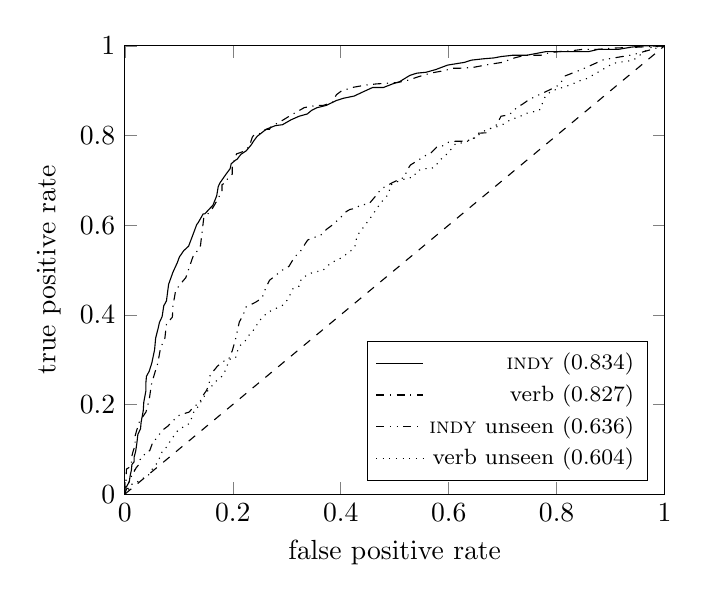
\begin{tikzpicture}
    \begin{axis}[xmin=0,xmax=1,ymin=0,ymax=1,xlabel={false positive rate},ylabel={true positive rate},legend pos=south east,legend cell align={right},legend style={font=\footnotesize}]
      \addplot [dashed,forget plot] coordinates{(0,0) (1,1)};
      \addplot [] coordinates{(0.000,0.000) (0.000,0.005) (0.000,0.016) (0.003,0.016) (0.005,0.021) (0.008,0.027) (0.010,0.043) (0.012,0.053) (0.013,0.066) (0.017,0.072) (0.017,0.082) (0.020,0.096) (0.022,0.112) (0.024,0.133) (0.029,0.146) (0.030,0.160) (0.034,0.186) (0.035,0.205) (0.037,0.218) (0.039,0.231) (0.039,0.247) (0.039,0.250) (0.040,0.263) (0.045,0.274) (0.050,0.293) (0.055,0.322) (0.057,0.348) (0.062,0.372) (0.064,0.383) (0.069,0.396) (0.072,0.420) (0.077,0.431) (0.081,0.468) (0.089,0.495) (0.097,0.516) (0.101,0.529) (0.109,0.543) (0.118,0.553) (0.124,0.572) (0.133,0.601) (0.136,0.606) (0.145,0.625) (0.148,0.625) (0.158,0.638) (0.163,0.644) (0.170,0.665) (0.173,0.686) (0.176,0.694) (0.187,0.713) (0.195,0.726) (0.197,0.737) (0.205,0.745) (0.208,0.747) (0.215,0.758) (0.225,0.766) (0.234,0.779) (0.240,0.790) (0.245,0.798) (0.262,0.814) (0.279,0.822) (0.292,0.824) (0.308,0.835) (0.323,0.843) (0.338,0.848) (0.346,0.856) (0.356,0.862) (0.373,0.867) (0.392,0.878) (0.405,0.883) (0.425,0.888) (0.439,0.896) (0.459,0.907) (0.479,0.907) (0.496,0.915) (0.509,0.920) (0.528,0.934) (0.541,0.939) (0.558,0.941) (0.576,0.947) (0.598,0.957) (0.629,0.963) (0.642,0.968) (0.664,0.971) (0.684,0.973) (0.697,0.976) (0.719,0.979) (0.745,0.979) (0.780,0.987) (0.797,0.987) (0.829,0.987) (0.859,0.987) (0.877,0.992) (0.914,0.992) (0.938,0.997) (0.961,1.000) (1.000,1.000)}; %indy auc = 0.834
      \addplot [dash dot] coordinates{(0.000,0.000) (0.000,0.005) (0.000,0.008) (0.000,0.008) (0.000,0.008) (0.000,0.011) (0.000,0.019) (0.000,0.021) (0.000,0.027) (0.002,0.029) (0.002,0.032) (0.002,0.037) (0.003,0.056) (0.010,0.061) (0.012,0.069) (0.013,0.085) (0.015,0.095) (0.019,0.109) (0.019,0.130) (0.022,0.143) (0.027,0.162) (0.039,0.183) (0.045,0.210) (0.049,0.244) (0.056,0.273) (0.061,0.292) (0.066,0.326) (0.074,0.347) (0.077,0.379) (0.088,0.395) (0.089,0.419) (0.094,0.454) (0.103,0.469) (0.113,0.483) (0.121,0.512) (0.128,0.536) (0.136,0.544) (0.140,0.554) (0.143,0.584) (0.146,0.615) (0.152,0.623) (0.158,0.631) (0.162,0.637) (0.167,0.647) (0.172,0.658) (0.180,0.676) (0.180,0.690) (0.189,0.698) (0.190,0.703) (0.199,0.714) (0.199,0.729) (0.204,0.751) (0.207,0.759) (0.219,0.764) (0.224,0.767) (0.231,0.777) (0.236,0.796) (0.239,0.801) (0.244,0.801) (0.253,0.806) (0.258,0.812) (0.264,0.814) (0.268,0.814) (0.271,0.820) (0.279,0.825) (0.291,0.833) (0.306,0.844) (0.325,0.857) (0.332,0.862) (0.354,0.867) (0.367,0.867) (0.384,0.873) (0.392,0.891) (0.401,0.899) (0.421,0.907) (0.444,0.912) (0.466,0.915) (0.505,0.918) (0.524,0.923) (0.544,0.931) (0.566,0.939) (0.589,0.944) (0.609,0.950) (0.621,0.950) (0.646,0.952) (0.672,0.958) (0.699,0.963) (0.722,0.973) (0.742,0.979) (0.771,0.979) (0.785,0.984) (0.803,0.987) (0.828,0.989) (0.848,0.992) (0.875,0.992) (0.907,0.995) (0.951,0.997) (1.000,1.000)}; %verb auc = 0.827
      \addplot [dash dot dot] coordinates {(0.000,0.000) (0.001,0.000) (0.001,0.005) (0.003,0.011) (0.004,0.013) (0.007,0.013) (0.007,0.019) (0.007,0.027) (0.011,0.039) (0.016,0.042) (0.018,0.054) (0.019,0.054) (0.021,0.059) (0.026,0.066) (0.028,0.077) (0.033,0.080) (0.038,0.093) (0.046,0.097) (0.053,0.120) (0.056,0.121) (0.065,0.135) (0.070,0.143) (0.080,0.152) (0.085,0.159) (0.099,0.175) (0.108,0.179) (0.119,0.183) (0.127,0.194) (0.139,0.205) (0.142,0.215) (0.151,0.231) (0.156,0.244) (0.158,0.267) (0.168,0.280) (0.171,0.285) (0.184,0.297) (0.192,0.300) (0.199,0.320) (0.204,0.341) (0.209,0.367) (0.212,0.384) (0.219,0.399) (0.224,0.417) (0.242,0.428) (0.254,0.437) (0.261,0.460) (0.268,0.477) (0.291,0.499) (0.304,0.508) (0.314,0.528) (0.326,0.543) (0.336,0.562) (0.339,0.567) (0.354,0.574) (0.363,0.578) (0.374,0.591) (0.383,0.599) (0.398,0.615) (0.410,0.630) (0.417,0.635) (0.429,0.638) (0.436,0.645) (0.452,0.647) (0.464,0.664) (0.475,0.681) (0.496,0.695) (0.518,0.707) (0.523,0.723) (0.529,0.734) (0.545,0.746) (0.555,0.754) (0.567,0.761) (0.578,0.774) (0.586,0.775) (0.600,0.785) (0.612,0.787) (0.623,0.787) (0.635,0.789) (0.646,0.791) (0.654,0.805) (0.670,0.806) (0.677,0.815) (0.689,0.824) (0.697,0.843) (0.712,0.846) (0.726,0.862) (0.737,0.870) (0.749,0.880) (0.759,0.886) (0.777,0.896) (0.791,0.904) (0.805,0.913) (0.816,0.933) (0.844,0.946) (0.887,0.969) (0.941,0.980) (1.000,1.000)}; %indy shuffled auc = 0.636
      \addplot [dotted] coordinates{(0.000,0.000) (0.000,0.004) (0.002,0.008) (0.006,0.009) (0.012,0.017) (0.012,0.022) (0.018,0.022) (0.026,0.030) (0.036,0.037) (0.042,0.039) (0.046,0.047) (0.052,0.058) (0.055,0.063) (0.061,0.071) (0.063,0.079) (0.067,0.084) (0.069,0.096) (0.079,0.107) (0.086,0.123) (0.091,0.130) (0.095,0.138) (0.102,0.146) (0.109,0.150) (0.120,0.158) (0.125,0.174) (0.129,0.188) (0.139,0.198) (0.142,0.211) (0.147,0.218) (0.149,0.226) (0.156,0.233) (0.166,0.249) (0.174,0.257) (0.182,0.265) (0.188,0.281) (0.192,0.296) (0.197,0.304) (0.205,0.304) (0.211,0.329) (0.222,0.340) (0.233,0.360) (0.242,0.370) (0.247,0.385) (0.258,0.396) (0.262,0.404) (0.278,0.413) (0.295,0.423) (0.303,0.437) (0.309,0.452) (0.312,0.460) (0.323,0.464) (0.327,0.481) (0.341,0.491) (0.352,0.496) (0.366,0.498) (0.382,0.516) (0.391,0.521) (0.401,0.527) (0.416,0.540) (0.426,0.551) (0.430,0.576) (0.445,0.600) (0.456,0.618) (0.465,0.634) (0.473,0.648) (0.489,0.670) (0.492,0.689) (0.499,0.694) (0.513,0.701) (0.536,0.708) (0.540,0.720) (0.552,0.726) (0.567,0.726) (0.576,0.731) (0.582,0.744) (0.589,0.750) (0.598,0.760) (0.613,0.782) (0.629,0.784) (0.642,0.791) (0.655,0.801) (0.671,0.814) (0.686,0.818) (0.701,0.825) (0.713,0.834) (0.733,0.843) (0.743,0.849) (0.757,0.853) (0.768,0.856) (0.779,0.887) (0.790,0.899) (0.816,0.909) (0.828,0.914) (0.840,0.921) (0.856,0.927) (0.875,0.940) (0.905,0.961) (0.942,0.968) (0.973,0.996) (1.000,1.000)}; %verb shuffled auc = 0.604
      \legend{\textsc{indy} (0.834),verb (0.827),\textsc{indy} unseen (0.636),verb unseen (0.604)} 
    \end{axis}
  \end{tikzpicture}
\caption[Receiver Operating Characterisation for Coercion Classification]{Receiver operating characteristic plots for a selection of models for coercion classification, with the area under the curve for each model type indicated in the legend.}
\label{fig:coerroc}
\end{figure}

Figure~\ref{fig:coerroc} presents a receiver operating characteristic plot comparing between the verb-only and \textsc{indy} techniques for both the regular and rearranged versions of the data at 400 dimensions with 2x2 word windows, with areas under the curve indicated in the legend.  As expected, the verb-only and \textsc{indy} techniques are comparable for the unaltered version of the data, but the model learned from verb-only subspaces falls off once each verb stem is treated as its own fold of the data.  Of particular note is the way that the rearranged verb-only curve flattens out in the middle: the relative drop-off in true positives in the mid-range of cut-off points for classifying coercion tells us that there is a lull in the precision of the model here, with mistakes being made on the interpretation of subspaces projected by unfamiliar verbs (keeping in mind that, in the unaltered version of the data, the subspace projected by two different instances of the same verb morpheme would be identical, and so it is only the variance in the relative situation of the noun-vector in these subspaces that needs to be analysed to evaluate coercion).  The relative jumpiness of the curves as compared to the smooth trajectories observed for the metaphor data in Figure~\ref{fig:metaroc} can be attributed to the scale of the data, with the massiveness of the metaphor dataset providing a steadier progression as the criteria for positive classification are relaxed.  On the whole, though, the story here is a similar one of a fairly balanced advance of recall and a correspondingly steady decline in precision as the model becomes increasingly permissive in its classification of coercion.

\subsection{The Geometry of Coercion}
Following the procedure which has proved productive for the analysis of semantic phenomena in preceding experiments, I will now study the statistical geometry associated with the contextual classification of coercion, beginning with an analysis of individual features and moving on to a consideration of optimal combinations of features.  In Table~\ref{tab:ind-coercion}, I once again report the top five performing (in terms of f-score) features for each of the context sensitive dimension selection techniques described in the previous section.  These features have been tested on the more prohibitive version of the coercion data rearranged to avoid training and testing on the same verb stem types, and with this in mind the improvement in scores here as compared to Table~\ref{tab:verb-coercion} is remarkable.  With the exception of the \textsc{zipped} subspaces, all other techniques exhibit substantial improvements on the models learned from the full set of statistical features, with the difference in the verb-only spaces especially notable and a substantial improvement with the chance of the results being randomly attained at $p = .070$.

\begin{table}
\centering
\begin{tabular}{lr|lr|lr}
\hline
\multicolumn{2}{c}{\textsc{joint}} & \multicolumn{2}{c}{\textsc{indy}} & \multicolumn{2}{c}{\textsc{zipped}} \\
\hline
$\mu(\overline{A'X'},\overline{B'X'})$ & 0.526 & $\mu(\overline{A'X'},\overline{B'X'})$ & 0.547 & $\mu(\overline{A'C'},\overline{B'C'})$ & 0.392 \\
$\mu(\overline{A'C'},\overline{B'X'}$ & 0.496 & $\mu(\overline{A'C'},\overline{B'C'})$ & 0.544 & $\mu(A,B)/C$ & 0.349 \\
$\mu(\overline{A'M'},\overline{B'M'}$ & 0.453 & $\mu(A,B)/C$ & 0.522 & $\mu(\overline{A'X'},\overline{B'X'})$ & 0.321 \\
$\mu(A,B)/C$ & 0.442 & $\angle AOB$ & 0.517 & $\mu(\overline{A'M'},\overline{B'M'})$ & 0.237 \\
$\angle AOB$ & 0.429 & $\mu(\overline{A'M'},\overline{B'M'})$ & 0.504 & $\angle AOB$ & 0.209 \\
\hline
\end{tabular}
\vfill
\begin{tabular}{lr|lr}
\multicolumn{2}{c}{\textsc{verb}} & \multicolumn{2}{c}{\textsc{noun}} \\
\hline
$\overline{AC}/\overline{BC}$ & 0.580 & $A:B$ & 0.528 \\
$A:B$ & 0.412 & $A/B$ & 0.486 \\
$A/B$ & 0.387 & $\mu(A,B)/C$ & 0.486 \\
$\mu(\overline{A'M'},\overline{B'M'})$ & 0.384 & $\angle AMB$ & 0.427 \\
$\mu(\overline{A'X'},\overline{B'X'})$ & 0.374 & $\angle ACB$ & 0.423 \\
\hline
\end{tabular}
\caption[Top Independent Features for Coercion Classification]{Independent f-scores from the coercion classification data for top five features of each subspace type for 2x2 word co-occurrence window, 400 dimension subspaces, validated on unobserved verbs.}
\label{tab:ind-coercion}
\end{table}

Also of note is the character of the features that are most predictive for each dimensional selection technique.  For all three methods involving both words as input for subspace selection, the mean values of distances at the normalised level of subspaces feature prominently (and it should be noted that the angle $\angle AOB$, which also features here, is perfectly correlated with the distance between the normalised word-vectors $A'$ and $B'$).  This indicates that the angles formed between the word-vectors and the generic vectors are especially associated with coercion, and this as opposed to metaphor, where the distance of various vectors from the origin as well as the ratios of these distances are particular predictive.  That the averages of the angles with the generic vectors seem generally more significant than the angles between the word-vectors themselves is evidence that it is the absolute and combined situation of the word-vectors in the context of their subspaces, rather than their relationship to one another, that can be interpreted in terms of a typological semantic relationship such as coercion.

All of this is in opposition to the top features for the subspaces selected based on a single input term, where fractions and ratios are prominent.  Of particular note is the significance of the relationship between the word-vectors, and this makes sense: given that the relevance of one word-vector in a subspace selected by the other is only incidental and in no way built into the space itself, differences in the relative lengths of the word-vectors and their relative distances to generic points are particularly indicative of degrees of inclusion in the profile characteristic of the dimension-selecting term.  The implication is that, with a co-occurrence profile chosen by one word, it is simply the prominence of the other word with respect to this profile that is indicative of the typological relationship between the verb's selectional constraints and the noun's categorical expectation.  Furthermore, the resurgence of verb-only spaces here in terms of a singular feature, namely, the fraction of the verb-centre-vector distance $\overline{AC}$ to the comparable distance $\overline{BC}$, tells us that the comparative situation of the word-vectors to the absolute centre of a subspace varies between coercive and non-coercive cases of argument selection.  It's worth noting here that, in verb-selected subspaces projected from the 2x2 word window base space, co-occurrence dimensions will correspond to terms that tend to be observed in close proximity to the verbs themselves, so we can expect these dimensions to be characterised by arguments of the verbs and modifiers of those arguments: it isn't hard to imagine how, in terms of modifiers in particular, the typical characteristics of the arguments normally selected by a verb would serve as a kind of template for testing the typological fit of a new candidate argument, with relative proximity to the centre, along with the extent of the noun vector along these characteristic co-occurrence dimensions, being good metrics for determining the fit.

\begin{table}
\centering
\begin{tabular}{llr}
\hline
& \multicolumn{1}{c}{\textsc{indy} ($f = 0.681$)} & \multicolumn{1}{c}{\textsc{verb} ($f = 0.688$)} \\
\hline
& \multicolumn{2}{c}{\textsc{distances}} \\
word-vectors & - & - \\
generic vectors & - & $-0.833 = X$ \\
\hline
& \multicolumn{2}{c}{\textsc{angles}} \\
word-vectors & $\angle AMB = -0.564$ & - \\
& $\angle ACB = -0.103$ \\
normalised & - & $0.290 = \angle A'M'B'$ \\
generic & - & $1.241 = \angle COM$ \\
& & $-0.214 = \angle COX$ \\
\hline
& \multicolumn{2}{c}{\textsc{means}} \\
word-vectors & $\mu(A,B) = 1.656$ & - \\
normalised & - & $0.452 = \mu(\overline{A'X'},\overline{B'X'})$ \\
\hline
& \multicolumn{2}{c}{\textsc{ratios}} \\
word-vectors & $\overline{AM}:\overline{BM} = 0.450$ & - \\
normalised - & - \\
\hline
& \multicolumn{2}{c}{\textsc{fractions}} \\
word-vectors & - & $2.315 = \overline{AM}/\overline{BM}$ \\
normalised & $\overline{A'M'}/\overline{B'M'} = -0.259$ & - \\
& $\overline{A'X'}/\overline{B'X'} = 0.203$ & - \\
generic vectors & $C/M = -1.257$ & $-2.398 = C/M$ \\
\hline
\end{tabular}
\caption[Most Predictive Feature Vectors for Coercion Classification]{Comparison of the seven most effective features for coercion classification in 2x2 word, 400 dimensional subspaces for \textsc{indy} versus \textsc{verb} based dimension selection.}
\label{tab:coertures}
\end{table}

These independent feature results are suggestive of the types of statistics that are associated with coercion, but not of the direction of these correlations, let alone the dynamics between different statistics.  To examine the geometry of coercion more in depth, I once again perform a beam search to discover the top seven features associated with both the \textsc{indy} and verb-only subspace selection techniques in 400 dimensional subspaces projected from 2x2 word window base spaces, training models on the rearranged version of the data and applying a vector inflation factor in order to avoid collinearity between input features.  Results are reported in Table~\ref{tab:coertures}.  Remarkably, a very different picture emerges than what was observed above regarding independent features, with neither the mean distances between the norms of the \textsc{indy} subspaces nor the angles and ratios individually observed in the verb-only subspaces making an appearance.  In fact, one of the most notable characteristics of the respective feature vectors is, on the one hand, the spread of the features across several different categories of co-occurrence statistic, but then also the balance between non-normalised features in one category for one technique versus the normalised components of the same category for the other technique.

So, for instance, the angles $\angle AMB$ and $\angle ACB$ both correlate negatively with coercion (meaning the angles are wider for more coercive word pairs) in the \textsc{indy} type subspaces, implying that the word-vectors are more likely to be found on opposite sides of these two central points in the space in the case of coercive pairings (but not necessarily on opposite sides of the lines extending from the origin through these points--they could, for instance, be above and below a point relative to the origin).  The positive correlation with the angle $\angle A'M'B'$ in the verb-only subspaces, on the other hand, indicates that the word-vectors tend to be on opposite sides of the lines extending through the mean vector.  This is interesting, since we can safely assume that the verb-vector will occupy a relatively central position in a subspace defined entirely by dimensions with which the verb has a high expectation of co-occurrence: it would seem that the noun-vector essentially pivots towards the co-occurrence dimensions that are most strongly associated with the verb, meaning that the words that are especially characteristic of the immediate syntagmatic situation of the verb tend to have a stronger association with nouns of a type not paradigmatically selected by the verb.  In the case of fractions of lengths between vectors, on the other hand, the very strong positive correlation between coercion and $\overline{AM}/\overline{BM}$ in verb-only spaces suggests that as the noun-vector (associated with $B$) retracts towards the origin relative to the verb-vector, coercion is more likely.  This makes sense in this type of subspace, since nouns of types that categorically satisfy a verb's selectional constraints will tend to have higher PMI values along the dimensions selected by that verb.  The negative value for the normalised version of the same fraction in the case of the \textsc{indy} subspaces, however, means that the respective angles between the word-vectors and the mean vector tend to be more balanced in cases of coercion.

The one point of consistent comparison across the two techniques is the fraction of the length of the central vector $C$ divided by the length of the mean vector $M$.  As discussed in Chapter~\ref{sec:litpare} in the context of the comparison between relatedness and similarity, the negative correlation here for both the \textsc{indy} technique and the verb-only technique indicates an increase in the likelihood of classifying a relationship as coercive as variance across the mean values of features delineating a subspace increases.  If high variance were only associated with coercion through the \textsc{indy} technique, it could be argued that coercion simply correlates with subspaces patched together from two different independently selected co-occurrence profiles with a tendency towards very different mean values: for instance, one word might select co-occurrence terms that occur more frequently and therefore have lower mean values than the other.  Given that this effect is even stronger for the verb-only subspaces, however, where the co-occurrence profile of just one term is in play, the prominence of this feature actually indicates that, as with similarity, there are some words (and, in particular, verbs) which just tend to be more coercive than others.  Moreover, these words tend to have a particular statistical characteristic by which the terms with which they co-occur tend to have more varied mean values.  In the end, this can be reduced to an observation that might not seem particularly surprising, even if it also wasn't immediately obvious prior to this geometric analysis: words that tend to be involved in coercive relationships also tend to co-occur with a range of other words that are more varied in terms of their own essential characteristics such as frequency.  This interpretation is further supported by the negative correlation between the length of the maximum vector $X$ and coercion in verb-only subspaces.  This generally indicates that there are some basic differences between the types of verbs, and the corresponding dimensional profiles, that tend to coerce their arguments, and specifically implies that coercive verbs tend to be observed in close proximity to at least some higher frequency words.

%verb joint shuffled f = 0.654

\begin{figure}
\footnotesize
\begin{subfigure}{0.3\textwidth} % heard noises
\centering
  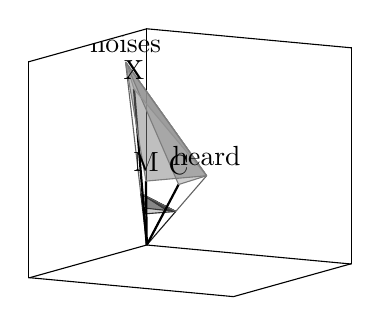
\begin{tikzpicture}
    \def\varA{(31.2371,41.3708,33.9778)};
    \def\varB{(64.4215,28.9478,79.8863)};
    \def\varC{(29.3997,29.3994,29.3996)};
    \def\varM{(36.4675,20.7482,30.9819)};
    \def\varX{(112.3873,59.9255,80.0081)};
    \def\varAN{(15.1191,20.0239,16.4456)};
    \def\varBN{(18.1248,8.1444,22.4758)};
    \def\varCN{(17.3206,17.3204,17.3205)};
    \def\varMN{(20.9761,11.9343,17.8207)};
    \def\varXN{(22.4161,11.9524,15.9580)};
    \def\nodA{31.2371,41.3708,33.9778};
    \def\nodB{64.4215,28.9478,79.8863};
    \def\nodC{29.3997,29.3994,29.3996};
    \def\nodM{36.4675,20.7482,30.9819};
    \def\nodX{112.3873,59.9255,80.0081};
    \begin{axis}[scale = 0.6,axis line style=white,view={120}{10},xmin=0,xmax=80,ymin=0,ymax=80,zmin=0,zmax=80,colormap/blackwhite,ticks=none]
      \addplot3[color=black,thick] coordinates {(0,0,80) (0,80,80)};
      \addplot3[color=black,thick] coordinates {(0,0,80) (80,0,80)};
      \addplot3[color=black,thick] coordinates {(0,80,0) (0,80,80)};
      \addplot3[color=black,thick] coordinates {(0,80,0) (80,80,0)};
      \addplot3[color=black,thick] coordinates {(80,0,0) (80,0,80)};
      \addplot3[color=black,thick] coordinates {(80,0,0) (80,80,0)};
      \addplot3[color=black] coordinates {(0,0,0) (0,0,80)};
      \addplot3[color=black] coordinates {(0,0,0) (0,80,0)};
      \addplot3[color=black] coordinates {(0,0,0) (80,0,0)};
      \addplot3[patch,patch type=triangle,color=gray,fill opacity=0.0] coordinates {(0.0,0.0,0.0) \varCN \varAN};
      \addplot3[patch,patch type=triangle,color=gray,fill opacity=0.0] coordinates {(0.0,0.0,0.0) \varCN \varBN};
      \addplot3[patch,patch type=triangle,color=darkgray,fill opacity=0.75] coordinates {\varCN \varAN \varBN};
      \addplot3[patch,patch type=triangle,color=darkgray,fill opacity=0.5] coordinates {\varMN \varAN \varBN};
      \addplot3[patch,patch type=triangle,color=darkgray,fill opacity=0.25] coordinates {\varXN \varAN \varBN};
      \addplot3 [color=black,thick] coordinates {(0,0,0) \varCN};
      \addplot3 [color=black,thick] coordinates {(0,0,0) \varXN};
      \addplot3 [color=black,thick] coordinates {(0,0,0) \varMN};
%      \addplot3[opacity = 0.1,surf,z buffer = sort,samples = 21,variable = \u,variable y = \v,domain = 0:90,y domain = 0:90,]
%    ({1*cos(u)*sin(v)}, {1*sin(u)*sin(v)}, {1*cos(v)});
      \addplot3 [patch,patch type=rectangle,color=lightgray,fill opacity=0.0] coordinates{\varAN \varA \varB \varBN
};
      \addplot3 [color=black,thick] coordinates {\varCN \varC};
      \addplot3 [color=black,thick] coordinates {\varXN \varX};
      \addplot3 [color=black,thick] coordinates {\varMN \varM};
      \addplot3 [patch,patch type=triangle,color=lightgray,fill opacity=0.75] coordinates{\varA \varC \varB};
      \addplot3 [patch,patch type=triangle,color=gray,fill opacity=0.25] coordinates{\varA \varX \varB};
      \addplot3 [patch,patch type=triangle,color=gray,fill opacity=0.5] coordinates{\varA \varM \varB};
      \node [anchor=south] at (axis cs: \nodA) {heard};
      \node [anchor=south] at (axis cs: \nodB) {noises};
      \node [anchor=south] at (axis cs: \nodC) {C};
      \node [anchor=south] at (axis cs: \nodX) {X};
      \node [anchor=south] at (axis cs: \nodM) {M};
    \end{axis}
  \end{tikzpicture}
\caption*{\footnotesize \emph{non-coercive: heard noises}}
\end{subfigure}
\hfill
\begin{subfigure}{0.3\textwidth} % hear click
\centering
  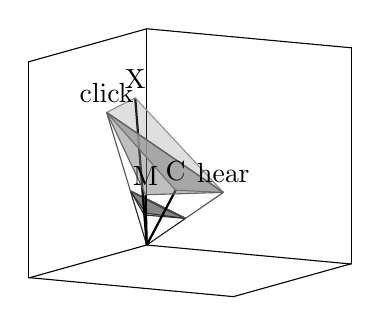
\begin{tikzpicture}
    \def\varA{(26.6923,45.2717,27.4741)};
    \def\varB{(45.5472,10.6624,56.8395)};
    \def\varC{(26.6298,26.6294,26.6297)};
    \def\varM{(34.7432,19.5859,25.5589)};
    \def\varX{(110.7493,59.4545,76.4383)};
    \def\varAN{(13.5030,22.9019,13.8985)};
    \def\varBN{(18.5620,4.3453,23.1640)};
    \def\varCN{(17.3206,17.3204,17.3205)};
    \def\varMN{(22.0031,12.4039,16.1866)};
    \def\varXN{(22.5841,12.1240,15.5874)};
    \def\nodA{26.6923,45.2717,27.4741};
    \def\nodB{45.5472,10.6624,56.8395};
    \def\nodC{26.6298,26.6294,26.6297};
    \def\nodM{34.7432,19.5859,25.5589};
    \def\nodX{110.7493,59.4545,76.4383};
    \begin{axis}[scale = 0.6,axis line style=white,view={120}{10},xmin=0,xmax=80,ymin=0,ymax=80,zmin=0,zmax=80,colormap/blackwhite,ticks=none]
      \addplot3[color=black,thick] coordinates {(0,0,80) (0,80,80)};
      \addplot3[color=black,thick] coordinates {(0,0,80) (80,0,80)};
      \addplot3[color=black,thick] coordinates {(0,80,0) (0,80,80)};
      \addplot3[color=black,thick] coordinates {(0,80,0) (80,80,0)};
      \addplot3[color=black,thick] coordinates {(80,0,0) (80,0,80)};
      \addplot3[color=black,thick] coordinates {(80,0,0) (80,80,0)};
      \addplot3[color=black] coordinates {(0,0,0) (0,0,80)};
      \addplot3[color=black] coordinates {(0,0,0) (0,80,0)};
      \addplot3[color=black] coordinates {(0,0,0) (80,0,0)};
      \addplot3[patch,patch type=triangle,color=gray,fill opacity=0.0] coordinates {(0.0,0.0,0.0) \varCN \varAN};
      \addplot3[patch,patch type=triangle,color=gray,fill opacity=0.0] coordinates {(0.0,0.0,0.0) \varCN \varBN};
      \addplot3[patch,patch type=triangle,color=darkgray,fill opacity=0.75] coordinates {\varCN \varAN \varBN};
      \addplot3[patch,patch type=triangle,color=darkgray,fill opacity=0.5] coordinates {\varMN \varAN \varBN};
      \addplot3[patch,patch type=triangle,color=darkgray,fill opacity=0.25] coordinates {\varXN \varAN \varBN};
      \addplot3 [color=black,thick] coordinates {(0,0,0) \varCN};
      \addplot3 [color=black,thick] coordinates {(0,0,0) \varXN};
      \addplot3 [color=black,thick] coordinates {(0,0,0) \varMN};
%      \addplot3[opacity = 0.1,surf,z buffer = sort,samples = 21,variable = \u,variable y = \v,domain = 0:90,y domain = 0:90,]
%    ({1*cos(u)*sin(v)}, {1*sin(u)*sin(v)}, {1*cos(v)});
      \addplot3 [patch,patch type=rectangle,color=lightgray,fill opacity=0.0] coordinates{\varAN \varA \varB \varBN
};
      \addplot3 [color=black,thick] coordinates {\varCN \varC};
      \addplot3 [color=black,thick] coordinates {\varXN \varX};
      \addplot3 [color=black,thick] coordinates {\varMN \varM};
      \addplot3 [patch,patch type=triangle,color=lightgray,fill opacity=0.75] coordinates{\varA \varC \varB};
      \addplot3 [patch,patch type=triangle,color=gray,fill opacity=0.25] coordinates{\varA \varX \varB};
      \addplot3 [patch,patch type=triangle,color=gray,fill opacity=0.5] coordinates{\varA \varM \varB};
      \node [anchor=south] at (axis cs: \nodA) {hear};
      \node [anchor=south] at (axis cs: \nodB) {click};
      \node [anchor=south] at (axis cs: \nodC) {C};
      \node [anchor=south] at (axis cs: \nodX) {X};
      \node [anchor=south] at (axis cs: \nodM) {M};
    \end{axis}
  \end{tikzpicture}
\caption*{\footnotesize \emph{neutral: hear click}}
\end{subfigure}
\hfill
\begin{subfigure}{0.3\textwidth} % hear motor
\centering
  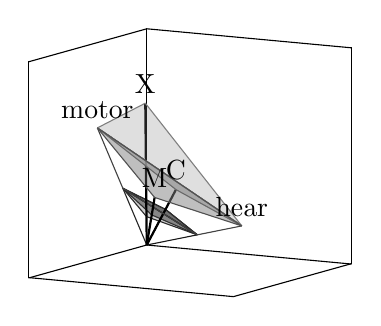
\begin{tikzpicture}
    \def\varA{(22.0152,49.7517,14.7908)};
    \def\varB{(37.5202,2.4240,49.1531)};
    \def\varC{(26.9425,26.9422,26.9425)};
    \def\varM{(33.6557,22.5056,24.6651)};
    \def\varX{(112.2882,64.2694,75.1433)};
    \def\varAN{(11.7145,26.4732,7.8703)};
    \def\varBN{(18.1889,1.1751,23.8282)};
    \def\varCN{(17.3206,17.3204,17.3206)};
    \def\varMN{(21.2972,14.2415,15.6080)};
    \def\varXN{(22.5149,12.8867,15.0670)};
    \def\nodA{22.0152,49.7517,14.7908};
    \def\nodB{37.5202,2.4240,49.1531};
    \def\nodC{26.9425,26.9422,26.9425};
    \def\nodM{33.6557,22.5056,24.6651};
    \def\nodX{112.2882,64.2694,75.1433};
    \begin{axis}[scale = 0.6,axis line style=white,view={120}{10},xmin=0,xmax=80,ymin=0,ymax=80,zmin=0,zmax=80,colormap/blackwhite,ticks=none]
      \addplot3[color=black,thick] coordinates {(0,0,80) (0,80,80)};
      \addplot3[color=black,thick] coordinates {(0,0,80) (80,0,80)};
      \addplot3[color=black,thick] coordinates {(0,80,0) (0,80,80)};
      \addplot3[color=black,thick] coordinates {(0,80,0) (80,80,0)};
      \addplot3[color=black,thick] coordinates {(80,0,0) (80,0,80)};
      \addplot3[color=black,thick] coordinates {(80,0,0) (80,80,0)};
      \addplot3[color=black] coordinates {(0,0,0) (0,0,80)};
      \addplot3[color=black] coordinates {(0,0,0) (0,80,0)};
      \addplot3[color=black] coordinates {(0,0,0) (80,0,0)};
      \addplot3[patch,patch type=triangle,color=gray,fill opacity=0.0] coordinates {(0.0,0.0,0.0) \varCN \varAN};
      \addplot3[patch,patch type=triangle,color=gray,fill opacity=0.0] coordinates {(0.0,0.0,0.0) \varCN \varBN};
      \addplot3[patch,patch type=triangle,color=darkgray,fill opacity=0.75] coordinates {\varCN \varAN \varBN};
      \addplot3[patch,patch type=triangle,color=darkgray,fill opacity=0.5] coordinates {\varMN \varAN \varBN};
      \addplot3[patch,patch type=triangle,color=darkgray,fill opacity=0.25] coordinates {\varXN \varAN \varBN};
      \addplot3 [color=black,thick] coordinates {(0,0,0) \varCN};
      \addplot3 [color=black,thick] coordinates {(0,0,0) \varXN};
      \addplot3 [color=black,thick] coordinates {(0,0,0) \varMN};
%      \addplot3[opacity = 0.1,surf,z buffer = sort,samples = 21,variable = \u,variable y = \v,domain = 0:90,y domain = 0:90,]
%    ({1*cos(u)*sin(v)}, {1*sin(u)*sin(v)}, {1*cos(v)});
      \addplot3 [patch,patch type=rectangle,color=lightgray,fill opacity=0.0] coordinates{\varAN \varA \varB \varBN
};
      \addplot3 [color=black,thick] coordinates {\varCN \varC};
      \addplot3 [color=black,thick] coordinates {\varXN \varX};
      \addplot3 [color=black,thick] coordinates {\varMN \varM};
      \addplot3 [patch,patch type=triangle,color=lightgray,fill opacity=0.75] coordinates{\varA \varC \varB};
      \addplot3 [patch,patch type=triangle,color=gray,fill opacity=0.25] coordinates{\varA \varX \varB};
      \addplot3 [patch,patch type=triangle,color=gray,fill opacity=0.5] coordinates{\varA \varM \varB};
      \node [anchor=south] at (axis cs: \nodA) {hear};
      \node [anchor=south] at (axis cs: \nodB) {motor};
      \node [anchor=south] at (axis cs: \nodC) {C};
      \node [anchor=south] at (axis cs: \nodX) {X};
      \node [anchor=south] at (axis cs: \nodM) {M};
    \end{axis}
  \end{tikzpicture}
\caption*{\footnotesize \emph{coercive: hear motor}}
\end{subfigure}
\caption[Coercion in Space]{Three dimensional projections of word-vectors and generic vectors in \textsc{indy} subspaces for pairs at the extents and in the middle of the spectrum of coercion.}
\label{fig:coerspaces}
\end{figure}

Figure~\ref{fig:coerspaces} illustrates word-vectors and generic vectors projected into exemplary instances of subspaces at three different phases of coercion.  Similarly to the literal stage of metaphor illustrated in Figure~\ref{fig:metaspaces}, the least coercive instance is characterised by a relatively tight space, with the noun-vector particularly prominent and acute angles at the vertexes of the generic points \revAK{2}{(and, also as with Figure~\ref{fig:metaspaces}, these are instances of exemplary word-pairs at either end and in the middle of the distribution of model output)}.  The next two stages of coercion go through something of the reverse of the process observed with metaphor, however, beginning with a retraction and a bit of a widening in the somewhat neutral case of \emph{hear click}, and then opening up into a more disparate arrangement across the subspace for the unambiguously coercive \emph{hear motor}.  The angles at the vertices of the generic point in particular, as well as the balance between the distances between the word-vectors and these points, follow the trend indicated by the coefficient weightings reported for \textsc{indy} subspaces in Table~\ref{tab:coertures}.  The shift in the overall balance of the word-vectors is interesting to note, as well: while the ratio $A:B$ wasn't indicated in the feature-wise analysis of the space, the prominence of the vector for \emph{noise} in the projection on the left suggests that there could be some nouns which are less likely to be susceptible to coercion, and indeed it is tricky to imagine the context in which the fairly abstract word \emph{noise} could be adapted to a conceptual category other than \textsc{noise}.

A more general implication of this geometric analysis is the idea that coercion is a graduated rather than a binary phenomenon.  This runs counter to what has been the conventional approach to this semantic phenomenon in the field, which considers coercion to be effectively an activation of a rule based process of constraint satisfaction: \cite{Pustejovsky1993} surveys the typical approach to coercion, and indeed to lexical ambiguity in general, as a process of contextualised \emph{selectional restriction} over a set of discrete word senses \citep[though see][for computational applications of a probabilistic, corpus based model]{LapataEA2003,ShutovaEA2013b}.  It seems apparent, though, that some instances of predicate type coercion are less obvious than others.  \emph{Hear click} illustrates this point nicely, as we are are forced to pause while we consider whether \emph{click} categorically denotes \textsc{noise} or something more like \textsc{process} or even \textsc{event}.  Furthermore, to borrow an instance from \cite{CopestakeEA1995}, among others, phrases such as \emph{enjoy a book} are clearly coercive and moreover open to interpretation as to the exact mechanism of type shifting: is the book being read or written?

The prodigious use of terms with tangible denotations such as \emph{book} in the literature suggests that the axis of concretion and abstraction may be involved in these determinations.  To the extent that concrete terms might be understood as relatively low level nodes in a conceptual taxonomy working its way up to the more abstract types, the distance of a word like \emph{motor} from a paradigmatic denotation such as \textsc{physical object} could therefore facilitate its coercion into the class \textsc{noise}.  Rather than modelling this semantic phenomenon as a consequence of a symbolic system of typed representations, however, I have sought to explore the extent to which co-occurrence features can prefigure subsequent high-level decisions about coercion.  To the degree that the output of my methodology can be considered a positive result, the finding might be summarised like this: there is evidence here for a lexical semantic model grounded in statistical, interactive, contextually adjustable representations, with categorical commitments regarding the conceptual indices of semantic units emerging from the dynamics of the representation in the course of language use.

\subsection{Adding Sentential Context}
To revisit \citepos{PustejovskyEA2008} hypothesis regarding the mechanisms of semantic type coercion, the explication of type shifts arises fundamentally in a conceptual and, accordingly, linguistic context.  While I have, as discussed in Chapter~\ref{sec:sensitivity}, endeavoured to treat context as a more generally cognitive rather than strictly textual phenomenon, one of the appealing things about the data provided by \cite{PustejovskyEA2010} is that the word pairs classified in terms of coercion are embedded in sentences, and these sentences do naturally offer the basis for some sort of conceptual handle on the interaction between predicate and object.  In this section, I will perform a final experiment on semantic type coercion in which the context of each sentence is provided to my models as an additional input for projecting co-occurrence subspaces in which the relationship between word-vectors and generic vectors can be analysed.

To begin with, I take each sentence and, using the Stanford Parser \citep{ToutanovaEA2000},\footnote{As provided by the \texttt{nltk} package for python.} extract a part-of-speech tag for each word in each sentence in the data.  (Note that, now that I'm using the full sentences which provide unique data for every word-pair, I can use full data set of 1,992 sentences.)  For each sentence, I group together all the words other than the target verb and object that satisfy one of four grammatical class descriptions: nouns, verbs, adjectives, and adverbs.  I then run four different experiments, one treating the words for each of these grammatical classes as the input for dimension selection and then analyse the situation of the word-vectors in the projected subspaces in terms of the now familiar catalogue of geometric statistical features.  I treat the output for each grammatical class as the data for a logistic regression, first applying standard mean normalisation and then, setting values for sentences where no words of a particular grammatical class are available to zero, train a model to learn to classify each word pair as coercive or not coercive.  Results for each grammatical class, with various dimensional and co-occurrence window parameters, using the \textsc{joint} and \textsc{indy} dimension selection techniques, are reported in Table~\ref{tab:poses}.

\begin{table}
\centering
\begin{tabular}{llrrrr|rrrr}
\hline
\multicolumn{2}{l}{\emph{window}} & \multicolumn{4}{c}{2x2} & \multicolumn{4}{c}{5x5} \\
\multicolumn{2}{l}{\emph{dimensions}} & 20 & 50 & 200 & \multicolumn{1}{c}{400} & 20 & 50 & 200 & 400 \\
\hline
\parbox[t]{2mm}{\multirow{4}{*}{\rotatebox[origin=c]{90}{\textsc{joint}}}} & nouns & 0.157 & 0.174 & 0.244 & \revAK{4}{\emph{0.283}} & 0.193 & 0.244 & 0.257 & \revAK{4}{\emph{0.271}} \\
& verbs & 0.121 & 0.155 & 0.190 & 0.237 & 0.117 & 0.163 & 0.215 & 0.229 \\
& adjectives & 0.083 & 0.113 & 0.179 & 0.187 & 0.119 & 0.131 & 0.183 & 0.207 \\
& adverbs & 0.042 & 0.091 & 0.155 & 0.154 & 0.101 & 0.128 & 0.171 & 0.174 \\
\hline
\parbox[t]{2mm}{\multirow{4}{*}{\rotatebox[origin=c]{90}{\textsc{indy}}}} & nouns & 0.092 & 0.133 & 0.147 & 0.157 & 0.158 & 0.170 & 0.148 & 0.168 \\
& verbs & 0.117 & 0.126 & 0.173 & 0.165 & 0.147 & 0.209 & 0.174 & 0.201 \\
& adjectives & 0.123 & 0.114 & 0.162 & 0.172 & 0.173 & 0.161 & 0.151 & 0.184 \\
& adverbs & 0.115 & 0.137 & 0.139 & 0.120 & 0.167 & 0.146 & 0.121 & 0.111 \\
\hline
\end{tabular}
\caption[Correlations for Part-of-Speech Based Subspaces]{F-scores for coercion detection in full featured subspaces based on \textsc{joint} and \textsc{indy} analyses of parts of speech found in each sentence containing a verb-noun pair.}
\label{tab:poses}
\end{table}

The scores here are, clearly, low, with the difference between the top score of $f = 0.283$ for nouns in the 2x2 word window, 400 dimensional \textsc{joint} subspaces and the minority class baseline of $f = 0.458$ approaching significance at $p = .020$.  Beyond that, it is notable that the \textsc{joint} subspaces perform substantially better that the \textsc{indy} subspaces (at $p = .056$ for the 2x2 word window, 400 dimensional noun subspaces).  This suggests that a coherent subspace representing the intersection of co-occurrence profiles across the instances of a given grammatical class found in a sentence, rather a subspace merged out of the divergent co-occurrences associated with each word independently, presents a more cohesive basis for the analysis of the conceptual relationship between a predicate and an object.  More to the point, though, it seems that sentential context, as far as this analytical technique is concerned, provides only marginal information for contextualising the relationship between a verb and the potentially shifted type of one of its arguments.  \del{Turning back to the data, the sentences analysed were extracted from the BNC corpus, and so in many instances have a particularly colloquial or conversational character} \revAK{21}{As the sentences analysed here were selected from the BNC, a balanced corpus of spoken and written English, some of these sentences can be conversational in character, and so arguable do not provide much contextualising information}: it is not clear how much useful additional co-occurrence context could be found in sentences such as, ``We will be \emph{denying} the \emph{charges} strongly in court,'' or, ``I mean the \emph{train} could have been \emph{cancelled} or something,'' or simply, ``He \emph{finished} his \emph{drink}.''  In the end, then, sentential context could easily be seen as activating other non-linguistic cognitive context that is not built into the type of statistical model explored here.

\revJB{3}{A more comprehensive approach to classifying coercion might involve projecting subspaces based on an analysis of both the words in the relationship being modelled and the corresponding sentential context.  The problem mentioned above, however, of some sentences providing significantly more information than others, would confound a straightforward attempt to simply concatenate statistics derived from each type of analysis: some features vectors of subspaces derived from word pairs would be coupled with significantly more informative sentential feature vectors than others.  A more productive and sophisticated version of such an approach could involve the establishment of a balanced interpretive input for any given sentence through, for instance, the application of a topic modelling technique such as latent dirichlet allocation} \citep{BleiEA2003}, \rev{which could associate any given sentence with a set number of key words.  This extension of the research presented here is one of the many directions worth considering for future applications of my context sensitive methodology.}

Finally, Table~\ref{tab:coerpare} presents the outcomes of models tested on the data as originally presented, split into a training and test set each containing instances of all five verb stems.  In addition to the top performing \textsc{indy} and verb-only subspaces, I present results for two different \emph{example based learning} techniques.  In the first instance, denoted \textsc{EBL}, a rule is learned for each verb stem type in the training data, based simply on whether that verb is usually observed to take a noun of the specified type as an argument or to coerce the type of its argument, and then that rule is applied across all instances in the test data.  In practice this means that forms of \emph{finish} are predicted to be coercive, and all other verbs are predicted to take arguments of the expected type.  The enhanced \textsc{EBL*} technique learns a rule for each verb-noun combination, resorting to the \textsc{EBL} rule when it encounters an unobserved pairing in the training data.  The very strong results here simply indicate that a large number of combinations are attested in both the training and test data, a peculiarity which I sought to overcome through the rearrangement of the data described above.

\begin{table}
\centering
\begin{tabular}{lrrrr}
\hline
& \emph{precision} & \emph{recall} & \emph{f-score} & \emph{accuracy} \\
\hline
\textsc{indy} & 0.708 & 0.603 & 0.651 & 0.805 \\
\textsc{verb} & 0.726 & 0.610 & 0.663 & 0.813 \\
\cite{RobertsEA2010} & - & - & - & 0.961 \\
\cite{RobertsEA2011} & - & - & - & 0.812 \\
\textsc{EBL} & 0.630 & 0.498 & 0.556 & 0.764 \\
\textsc{EBL*} & 0.833 & 0.690 & 0.755 & 0.871 \\
\textsc{minority class} & 0.291 & 1.000 & 0.458 & 0.297 \\
\textsc{majority class} & 0.000 & 0.000 & 0.000 & 0.703 \\
\hline
\end{tabular}
\caption[Coercion Scores Compared Against Other Methods]{Coercion scores for the best performing context sensitive methods trained and tested on the original data configuration and compared to various other results.}
\label{tab:coerpare}
\end{table}

I also survey the two results previously reported in the literature here.  \cite{RobertsEA2011} present a probabilistic model that assigns a likelihood to classes associated with both predicate arguments and nouns based on observations across a large scale corpus and then uses the training set of the SemEval data to learn to identify a threshold of coercion.  So, where my models learn something about the way that predicates and objects interact in different co-occurrence contexts, this model seeks to learn something about coercion based on dependency-enhanced distributions.  The similar accuracy scores suggest that in the end the two approaches are using different mechanisms to arrive at a similar sense of coercion outside of sentential context, though it would be interesting to compare precision and recall scores or even line-by-line model output in order to better understand the specific ways that each techniqe makes its determinations.  The superior results of \cite{RobertsEA2010} are based on a model which specifically extracts predicate argument expectations and noun classes from WordNet and combines these features with a number of other features, combining data driven approaches with knowledge bases.  The end result can be thought of as an enhancement on the \textsc{EBL*} technique described above.

Based on the results reported by \cite{RobertsEA2011}, we might reasonably speculate that building word-vectors based on dependency relationships -- for instance, treating the distance between words in a parse tree rather than absolute distance in a string as the boundary condition for co-occurrence window size, as \cite{PadoEA2007} have discussed -- might significantly enhance a model's ability to classify coercion.  But this would come at the expense of building a model that doesn't have some degree of syntactic commitment already built into it, and it is likewise easy to imagine how such an approach would open itself up to accusations of tautology: if coercion as a binary case is a grammatical abstraction, then such a model would be to some extent recapitulating the premise of coercion data structuring.  Of greater interest would be, in line with the degrees or axes of metaphoricity briefly explored in Section~\ref{sec:genaphor}, establishing data indicating novel or exceptional cases of coercion, or alternatively of coercion scored along a continuous scale.  This might require a reworking of the standard dogma of semantic type shifting, but then one of the objectives of my methodology is to provide a computational framework for exploring and possibly shifting the lines of theories about language and meaning.

%\begin{table}
%\centering
%\begin{tabular}{lrrrr|rrrr}
%\hline
%\emph{window} & \multicolumn{4}{c}{2x2} & \multicolumn{4}{c}{5x5} \\
%\emph{dimensions} & 20 & 50 & 200 & \multicolumn{1}{c}{400} & 20 & 50 & 200 & 400 \\
%\hline
%\textsc{joint} & 0.348 & 0.369 & 0.352 & 0.371 & 0.369 & 0.392 & 0.362 & 0.383 \\
%\textsc{indy} & 0.411 & 0.406 & 0.467 & 0.494 & 0.402 & 0.358 & 0.421 & 0.438 \\
%\hline
%\end{tabular}
%\caption[F-Scores for Coercion Classification Using Full Sentences]{F-scores for coercion identification using sentential context to generate additional subspaces and corresponding feature vectors.}
%\label{tab:full-coercion}
%\end{table}

\section{Interpretation and Composition in Context} \label{sec:intercomp}
One of the tricky things about figurative language is its ephemerality: if we stare at it for long enough through a theoretical lens, it seems to vanish, as is evident in the deflationary case made by \cite{SperberEA2012}.  But on the other hand, if we ask someone in street whether the phase \emph{buy a story} is more metaphoric than \emph{buy a book}, we can reasonably expect the answer will almost always be ``yes'', and it would be a mistake to dismiss the evidence that in a colloquial sense some compositions are clearly metaphoric, and others are clearly not.  This raises a challenging point with regard to the comparison between metaphor and coercion, the two instances of figurative language explored in this chapter: is metaphor perhaps to some extent a more overt case of coercion, or maybe a specific case that is in some way or another a little more subtle?  Part of the problem here is that the distinctions between these phenomena begin to exceed the capacity for what can reliably be quantified about language in a clinical setting, with evaluative criteria that will depend on the opinion of an expert which comes pre-packaged with inevitable biases.

The experiments presented in this chapter have focused on the classification of non-literal language: the simple task of determining whether the way that a set of words are used pertains to some encyclopaedic sense of their lexical semantic role, without regard to the explication of any sort of interpretation of how semantics are subverted or what the metaphor communicates.  But \cite{Shutova2010} has made the case that, in a cognitively plausible sense, metaphor classification should be seen precisely as metaphor interpretation, and this theoretical stance has been backed up by a data-driven computational model that involves classification of metaphor by way of a round-trip paraphrasing technique.  This in turn invites a consideration of the entanglement between the interpretation and composition of figurative language: metaphor and metonymy are things that, in some particular conceptual context, are done by one lexical entity to another, as the apt term \emph{coercion} would itself suggest.  If composition happens in some cognitive context, then interpretation presumably involves the identification or simulation of that context, as the relevance theoretical account of metaphor surveyed in Chapter~\ref{sec:words}.  So this is in line with \citepos{Carston2010} description of how metaphor involves the generation of an \emph{ad hoc} concept pertaining to the semantics of the shifted lexeme in the specific context of a particular linguistic encounter.

In fact, \del{it is tempting to go so far as to say} \revJB{4}{we might speculate} that, \revJB{4}{at least to a certain extent,} figurative language is identified \del{precisely} \revJB{4}{partly} as \del{those} instances of language where recourse to a conceptual context is necessary to interpret a lexical composition, and furthermore that the degree of figurativeness correlates with the extent of context construction involved in an interpretation.  If this postulate holds water, it means that figurative language is arguably about the perception of contextuality in the semantic complex that fulgurates between words and ideas as much as it is about the alignment of properties between conceptual domains.  \revJB{4}{This theoretical suggestion is to some extent backed up by psycholinguistic studies in which EEG tests have indicated increasing processing time in human subjects moving from the comprehension of literal to conventional and then unfamiliar instances of metaphor} \cite{ArzouanEA2007}.  Under this theoretical regime, my context sensitive methodology should offer a good framework for identifying figurative language, because models built using this methodology can be indicative of the extent to which contextualisation draws generic or encyclopaedic representations into alignment with one another.  This hypothesis is supported by the evidence from the metaphor experiments in Section~\ref{sec:metperiment}, where strong results for both metaphor classification and the translation of metaphor classification models to the task of rating metaphoricity on a continuous scale indicate that the relationship between lexical semantic concepts in context sensitive spaces does tell us something about the degree to which \emph{ad hoc} concepts are being extrapolated in the course of composing the input terms.

The lower numbers associated with the coercion results described in Section~\ref{sec:coerperiment}, and particularly to the detection of predicate argument coercion involving unattested verbs, are to some extent a natural product of the nature of the data, given that the data offered by \cite{PustejovskyEA2010} presents coercion as a minority case.  It's also worth considering, however, the way in which the theoretical framing of coercion seeks to impose a fairly rigid structure on the conceptual hierarchy inherent in lexical typing.  The presumption is broadly, in the specific case of predicate argument shifting examined here, that a given verb takes a singular class as its argument, and that noun sense are likewise defined in terms of distinct classes, and so coercion is in principle understood as a discretely binary phenomenon.  But there are clearly issues of hierarchy and level of abstraction at stake in making class distinctions with regard to the denotations of nouns, and in fact there are some instances of coercion -- ``cancel a train'', for instance, or ``hear a click'' -- where the conceptual shift, while perhaps strictly present according to a particular categorical lexicon, does not involve a significant conceptual reconstruction by way of contextualisation.

This, then, raises a valid question: is the role of figurative language exclusively, or even for that matter primarily, to port attributes from one conceptual domain to another?  Or is what metaphor does, as \cite{Davidson1978} has famously suggested, really about something more fundamentally phenomenological than just the efficient transmission of propositions?  So, where, for instance, \cite{Sweetser1990} sees polysemy as an intermediate stage bridging the progress from literal to metaphoric usage, my methodology leaves itself open to the possibility that all usage is, in fact, first and foremost pragmatic, and only secondarily lexicalised.  By this interpretation, words have semantic affordances in terms of their potential to convey cognitive content intersubjectively, and they are picked up and used in much the same way that a cognitive agent might adapt an object designed or just perceived as being for one purpose as an implement in another activity---using a shoe as a hammer, for example, or a chair to fend off a lion.  The cognitive foregrounding of this nascent theory can be found in the ecological psychology of \cite{Bateson1972} and \cite{Gibson1979}, and the linguistic correlary seems to be in line with what psycholinguists inspired by biosemiotics such as \cite{RaczasekLeonardiEA2015} are saying about the way that language is primarily about affording cognitive value to interlocutors, including but hardly limited to truth values.

This theoretical speculation is a potential extrapolation of my methodology rather than a precondition for it, and is offered primarily as an example of how this statistical approach might become a component of productive line of philosophical enquiry.  The point, though, is that with a geometric methodology, relationships between lexical semantic representations can be recast as Gibsonian affordances: there is a mechanism for the direct perception of opportunities for meaning making in the actual layout of the statistical environment.  Meaning is, then, something which is directly perceived and acted upon, in the sense that a geometric mode of representation allows us, in an abstract sense, to imagine how an agent might participate in symbolically grounded semantic activity without resorting to the computation of the conceptual transpositions involved in the analysis of figurative language.  \revJB{5}{By this stipulation, meaning arises not so much from an exploration of a semantic space, as through the contextual generation of a space in which useful and potentially unexpected opportunities for communication and representation present themselves.}  By situating semantic representations in situationally induced spaces, the probabilisitic contingencies between words in particular contexts can in principle be mapped directly to the perception of an opportunity for meaning making without the need to resort to an interposing layer of conceptual computation.  It would be a mistake to go any further than this in terms of arguing for the cognitive plausibility of a model that is fundamentally statistical and computational, but, inasmuch as it it a desirable thing to consider the possibility that the prolific use of metaphor in the course of ordinary linguistic communication is an artefact of a more general cognitive propensity to grab whatever is available in an environment and make use of it, the methodology described here seems like an acceptable starting point for further investigation.


\chapter{The Geometry of Conceptualisation: Analogies} \label{chap:analogy}
In this chapter, as a final empirical investigation into the potentialities of context specific distributional semantic techniques, I will investigate the capacity of my methodologies to model analogy.  For the purposes of the computational and geometric modelling of semantics, analogy can be seen as a kind of meta-phenomenon: an analogical equation involving two sets of lexical representations indicates that there is some underlying intensionality that conceptually binds the denotations of the representations.  So, for instance, the metaphor ``that surgeon is a butcher'' can be extended through a mapping between the conceptual domains of \textsc{surgery} and \textsc{butchery} to arrive at semantic formulae such as \emph{surgeon:scalpel :: butcher:cleaver} or \emph{hospital:patient :: abattoir:carcass}.  Furthermore, if these relationships can be mapped geometrically in a semantic space, then we should have on our hands a productive mechanism for configuring a general semantic model---and one which may overcome some of the issues of interpretation and composition raised in the last chapter.  If we can connect a general region of butchery to a region of surgery in a semantic space, for instance, then we might be able to extrapolate such metaphoric turns of speech as ``the surgeon hacked at me with her scalpel'' from a model without committing to the claim that the model (or, for that matter, an agent) has actually interpreted the metaphor in an online way.

The idea that there is a geometric component to analogy is at least hinted at by \cite{Tversky1977}, who, as discussed in Chapter~\ref{sec:frames}, raises the issue of inequalities and asymmetries in relationships of synonymy.  \cite{Gentner1983} extends Tversky's insights to a model explicitly targeting analogy through the application of isomorphic \emph{structure mappings} that identify congruities between conceptual domains based on composite symbolic representations.  From a computational perspective, \cite{VealeEA1992} describe a system that functions through a series of \emph{spatial operators} which facilitate mappings between conceptual domains by way of a schema of collocations, containments, and orientations, though these operations do not involve the instantiation of Euclidean measures.  Subsequent symbolic computational models of metaphor in particular have seized on the mechanism of modelling mappings between conceptual structures that are, to a greater or lesser extent, based on the identification of congruities and a corresponding geometrical logic of sorts, and a small sample of work in the field has been surveyed in Chapter~\ref{sec:words} and \ref{sec:metaback}.

The empirical work described here will, naturally, focus on a statistical rather than symbolic approach to modelling analogy by way of spatial mappings between domains---and, in this case, domains, in the spirit of \cite{Gardenfors2000}, are represented roughly as regions in a Euclidean space.  It is important to note, though, that one of the primary components of the productive symbolic approaches to analogy mentioned above goes away once we move into distributional semantic spaces: where the features of symbolic representations are generally constructed to be interpreted as actual attributes of the denotations being modelled, the dimensions of distributional semantic spaces are simply indices to information about co-occurrences observed in a digital corpus (this has already been discussed in Chapter~\ref{sec:litdims} in the context of \citepos{Rimell2014} work studying the relationship between co-occurrence overlap and entailment, and again in Chapter~\ref{sec:interpretable} by way of \citepos{DerracEA2015} model treating directions in factorised distributional spaces as conceptual themes).  So there is a trade-off between access to a continuous Euclidean space of lexical semantic representations with geometric measures facilitated by the statistical nature of the representation building process and the loss of interpretable features in a symbolic conceptual scheme.  My hypothesis here, in line with experiments described in the previous two chapters, is that a process of contextualisation can generate spaces where collections of co-occurrence dimensions representing conceptually oriented profiles of language use will provide an appropriate ground for modelling analogy in terms of rigorous Euclidean relationships.  And in the case of analogy in particular, as will be seen in the following section, there is already a body of work offering compelling evidence that distributional semantic statistics can map conceptual relationships onto the geometry of word co-occurrence.

\section{Analogies as Parallel Vectors} \label{sec:parallel}
The \texttt{word2vec} distributional semantic modelling techniques, which have served as a point of comparison and discussion throughout this thesis, were originally presented with a test set of 19,544 four-word analogies, constructed by the model artchitects and devised to cover a range of relationships which the designers categorised as broadly \emph{semantic} or \emph{syntactic} \citep{MikolovEA2013b,MikolovEA2013c}.\footnote{The analogy data is included in the package that can be downloaded at \url{https://code.google.com/archive/p/word2vec/source/default/source}.}  So, for instance, the data presents relationships such as, on the one hand, \emph{Bangkok:Thailand :: Paris:France} or \emph{boy:girl :: man:woman}, and, on the other hand, \emph{calm:calmly :: lucky:luckily} or \emph{aware:unaware :: efficient:inefficient}.  The task involves feeding a semantic model the first three terms and then measuring the rate at which it is able to accurately predict the fourth term.

The neural network architecture of the \texttt{word2vec} approach produces remarkably strong results on this task through the application of a simple geometric device.  Within the normalised space of word-vectors generated over the course of iterative traversals of a large-scale digital corpus, given an unfinished analogy of form \emph{A:B::C:X}, the model simply finds the vector $\overrightarrow{x}$ most closely fulfilling the equation $\overrightarrow{b} + \overrightarrow{c} - \overrightarrow{a} \approx \overrightarrow{x}$, where $\overrightarrow{a}$, $\overrightarrow{b}$, and $\overrightarrow{c}$ are the word-vectors corresponding to the three known elements of the analogy, and returns the vocabulary word associated with $\overrightarrow{x}$.  The original literature reports an accuracy rate of 0.61 for the CBoW model, which is all the more impressive when we consider how many ways there are to choose the wrong solution to an analogy from a vocabulary of one million words.  \citep[It should be noted that similarly strong results have been reported for the hybrid frequentist-neural model of][.]{PenningtonEA2014}

But the really remarkable thing about these results is that the models build these spaces in a completely unsupervised manner with respect to the actual task of analogy solution.  This means that the arrangement of word-vectors plays out in a tidy conceptual geometry, interpretable through simple linear algebraic operations, simply by virtue of the way that words tend to come up in proximity to one another in the course of colloquial written language use (the original results were obtained from models trained on the Google News Corpus, and, as will be seen below, the same models trained on Wikipedia achieve comparable scores).  Much has been made of this: \cite{LevyEA2014} postulate about the procedural equivalence of iterative and statistical models mitigated by parameterisation issues, while \cite{AroraEA2015} have attempted to explain mathematically how the application of a random walk type algorithm to statistical models results in a recapitulation of the strong neural network results.  At the time of writing, there is a generally accepted intuition afoot in the field that, along the lines of the distributional hypothesis itself, it makes sense that the gradual nudging of word-vectors by a neural network based on observations of co-occurrences should push words into situations where orientations and distances in space broadly map to conceptual relationships between representations; there is not, however, a well-formed mathematical explanation of why these techniques are so effective at projecting semantic relationships into space.  At any rate, the import of all this is that, in \texttt{word2vec} type distributional semantic spaces, at least a certain type of analogy plays out along the lines illustrated in Figure~\ref{fig:sense}, as a close approximation of a parallelogram at the surface of a normalised hypersphere in a space delineated by abstract dimensions acting as handles for the backpropagating action of a neural network.

\begin{figure}
%  \centering
  \begin{subfigure} [t] {0.5\textwidth}
  \centering
  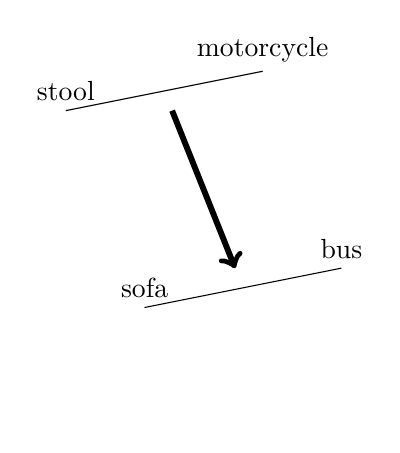
\begin{tikzpicture} [scale = 0.05]
    \draw (10,80)--(60,90);
    \draw (10,80) [above] node {stool};
    \draw (60,90) [above] node{motorcycle};
    \draw (30,30)--(80,40);
    \draw (30,30) [above] node {sofa};
    \draw (80,40) [above] node {bus};
    \draw [->,line width = 0.75 mm] (37,80)--(53,40);
    \draw (60,10) [below,white] node {soft};
  \end{tikzpicture}
  \caption{This makes sense.}
  \label{fig:sense}
  \end{subfigure}
  \begin{subfigure} [t] {0.5\textwidth}
  \centering
  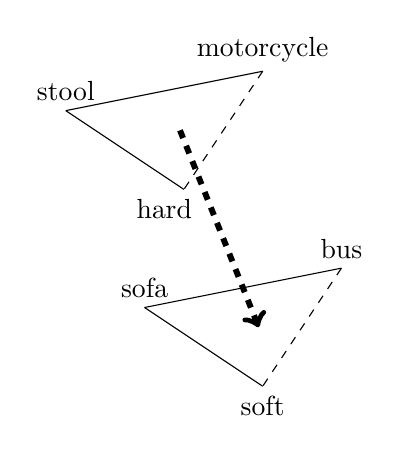
\begin{tikzpicture} [scale = 0.05]
    \draw (10,80)--(60,90);
    \draw (10,80)--(40,60);
    \draw [dashed] (60,90)--(40,60);
    \draw (10,80) [above] node {stool};
    \draw (60,90) [above] node {motorcycle};
    \draw (35,60) [below] node {hard};
    \draw [->,line width = 0.75 mm,dashed] (39,75)--(59,25);
    \draw (30,30)--(80,40);
    \draw (30,30)--(60,10);
    \draw [dashed] (80,40)--(60,10);
    \draw (30,30) [above] node {sofa};
    \draw (80,40) [above] node {bus};
    \draw (60,10) [below] node {soft};
  \end{tikzpicture}
  \caption{Does this make sense?}
  \label{fig:nonsense}
  \end{subfigure}
\caption[Analogies Straining Geometry]{The analogical components of overlapping conceptual frames do not necessarily map neatly into a singular space.}
\label{fig:mismatch}
\end{figure}

So, to put it in plain language, the line between two points representing a conceptual relationship in one region of the space should be parallel to and in the same direction as two points in another region representing an analogous conceptual relationship under a different overall conceptual scheme.  There is, however, an objection to be raised here.  Returning once again to \citepos{Tversky1977} observations about the asymmetry of similarity, there are problems once we begin to extend the geometry of analogy to more complex conceptual structures, as illustrated in Figure~\ref{fig:nonsense}: for any given mapping between anything other than the most trivial conceptual domains, there will be some intensional component of the denotation that does not conform to the presumed isomorphism of the analogy in a distributional semantic space.  So, while it may be possible to map relatively atomic elements analogically in a space of fixed semantic points, it seems there will always be a breakdown when it comes to trying to discover isomorphisms between entire domains.

As will be recalled from Chapter~\ref{sec:frames} and the example involving moethers, nurses, and frogs, \cite{ChenEA2017} have noted geometrical anomalies specifically in the context of distributional semantics, demonstrating that the presumption of conceptual parallelism is considerably more consistent in some domains than others, and further using clinical studies on human respondents to feel out some of the disconnects in analogical chains inherent in these types of semantic models.  What becomes clear is that static distributional models are very effective at providing a semantically productive geometry some of the time, but they lack the adaptability that is fundamental to environmentally situated cognition and so do not make the open-ended kind of connections between words and concepts that are characteristic of semantics.  What is necessary is an element of flexibility, and I propose that my methodology for contextualising semantic spaces offers the proper kind of framework for providing the required sensitivity to unfolding situations in the world.

\section{Contextualising Analogical Geometry} \label{sec:anatext}
In this section, I will explore the distributional contexts of analogical semantic relationships.  The premise of this investigation arises from the disconnect illustrated in Figure~\ref{fig:mismatch}: it seems impossible to imagine how a static semantic space could consistently represent analogies as well-formed geometric entities.  Rather, I maintain that analogy is always to at least a certain extent context specific.  Following on this, my hypothesis is that there should almost always be some contextualisation which permits the satisfactory mapping of an analogy in a semantic space.  In the case of a simple four word lexical construct, which will be the focus of the work presented here, this means that an analogy is modelled as a parallelogram, with each of the word-vectors denoting the components of the analogy as a vertex, to a degree of precision that precludes any other word-vector from being mistaken as a component of the lexical-conceptual complex.

The empirical work described here will proceed initially with a strategy of reverse engineering of sorts, seeking to validate the possibility of discovering the kind of spaces that we would like to find for mapping analogies through contextualising operations on distributional semantic spaces delineated by literal co-occurrence dimensions.  This will lead on to an examination of some of the ways that context sensitive approaches might be applied to an analogy completion task, though, not surprisingly, it turns out to be considerably easier to find a space where an analogy works out as desired than to discover an analogy in the sizeable state space of possible subspaces.  In the end, this last empirical component to my research, which expands upon work originally presented in \cite{McGregorEA2016}, will hopefully serve as an incipient to further research in terms of the potentialities and capacities of context sensitive distributional semantics.

\subsection{Projecting Probability into Space} \label{sec:anamath}
Before we engage with an exploration of the analogical potential of context specific subspaces, a brief review of the mathematics of distributional semantic spaces with literal co-occurrence dimensions will serve to reinforce the connection between the geometry of analogy and the probabilistic grounding of my methodology.  Returning to the definition of a co-occurrence statistic outlined in Chapter~\ref{sec:math}, recall that the pointwise mutual information between a word $w$ and a co-occurrence term $c$ is the unexpectedness associated with an observation of $c$ in proximity to $w$, which can be expressed in terms of joint and compound probabilities (and the equation is approximate because we're ignoring the skewing factor of 1 and the smoothing constant described in Chapter~\ref{sec:pmi}):

\begin{equation}
PMI(w,c) \approx \log\left(\frac{p(w,c)}{p(w) \times p(c)}\right)
\end{equation}

\noindent The basic assumption of the geometric approach to analogy, meanwhile, is that the components of an analogy map into a parallelogram sitting in some askance situation in a high dimensional space, a state of affairs which can be expressed using linear algebraic terms for a suppositional analogy \emph{A:B::C:D} and the corresponding word-vectors:

\begin{equation}
\overrightarrow{a} - \overrightarrow{b} \approx \overrightarrow{c} - \overrightarrow{d}
\end{equation}

\noindent For any arbitrary dimension $i$, this can then be reduced to a difference between logs:

\begin{equation}
\log\left(\frac{p(a,i)}{p(a) \times p(i)}\right) - \log\left(\frac{p(b,i)}{p(b) \times p(i)}\right) \approx \log\left(\frac{p(c,i)}{p(c) \times p(i)}\right) - \log\left(\frac{p(d,i)}{d(a) \times p(i)}\right)
\end{equation}

\noindent This expression can be significantly reduced by merging the arguments of the logarithms on either side of the equation into ratios and then dropping the logs:

\begin{equation}
\frac{p(a,i) \times p(b)}{p(b,i) \times p(a)} \approx \frac{p(c,i) \times p(d)}{p(d,i) \times p(c)}
\end{equation}

\noindent Or, converting the ratio of joint and independent probabilities to conditional probabilities and with a little more algebra:

\begin{equation}
p(i|a,i|d) \approx p(i|b,i|c)
\end{equation}

\noindent To again state this plainly, our analogy optimisation function seeks to find those dimensions where the combined probability of observing a given co-occurrence term in the context of $A$ and also (though not necessarily simultaneously) $D$ is as close as possible to observing the same term in the contexts of $B$ and $C$.  So for instance we are interested in discovering a dimension that is about as likely to occur in a context of \emph{surgeon} and \emph{cleaver} as it is to occur in a context of \emph{butcher} and \emph{scalpel}.  If we can discover a profile of such dimensions, then we can productively map this particular analogy onto a contextualised distributional semantic space.

This property of semantic spaces defined in information theoretical terms is an artefact of the conversion of products and ratios into sums and differences through the mechanism of logarithmic functions.  To coin a term, logarithms \emph{geometrise} a space of probabilistic statistics, allowing us to perform operations on shapes in Euclidean space that correspond to hypotheses about joint and conditional observations of events, in this case co-occurrence events in a large scale corpus.  It must be emphasised, however, that the interpretability of probabilities in geometric terms only holds in spaces where dimensions still map to literal co-occurrence statistics, and so this property is a feature of my methodology but not of semantic spaces that have been factorised or learned through the abstract operations of a neural network.  The next objective, then, is to search for the appropriate techniques for specifying a context in order to map out a given analogy.

\subsection{Finding Contexts for Analogies}
I next investigate whether or not co-occurrence dimensions satisfying the conditions laid out above can be discovered in co-occurrence subspaces contextualised using the methods developed and explored throughout this thesis.  In particular we are interested in discovering the dimensions which most closely satisfy the equation $(\overrightarrow{a} - \overrightarrow{b}) - (\overrightarrow{c} - \overrightarrow{d}) = 0$ for the word-vectors corresponding to the components of the analogy \emph{A:B::C:D}.  This relationship can be examined on a dimenion-by-dimension basis, beginning by extracting dimensions that are known to have non-zero values for some or all of the word-vectors involved in the analogy.  Figure~\ref{fig:histograms} presents a histographic analysis of just such an analysis for two different analogies: the aforementioned \emph{surgeon:scalpel :: butcher:cleaver}, representing the frequently discussed conceptual mapping from \textsc{surgery} to \textsc{butchery}, and, from Figure~\ref{fig:mismatch}, \emph{stool:sofa :: motorcycle:bus}, indicating a mapping from \textsc{furniture} to \textsc{vehicles}.  In both cases the best three dimensions for satisfying the balance of values indicating parallel relationships between the legs of the analogy are selected from the top 400 dimensions projected from 5x5 word co-occurrence window based spaces taking the first three of the four components of each analogy as input to the \textsc{zipped} methodology.

\begin{figure}
\begin{subfigure} {1 \textwidth}
\centering
\begin{subfigure} [t] {0.3 \textwidth}
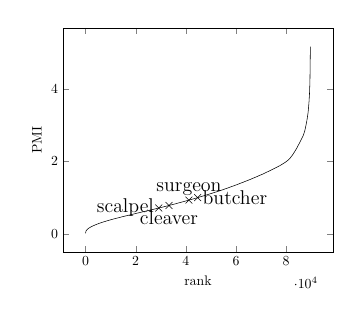
\begin{tikzpicture}[scale=0.5]
	\begin{axis} [xlabel=rank,ylabel=PMI]
	\addplot [mark=none] coordinates {
		(0,0.00622) (179,0.06993) (358,0.08958) (537,0.1038) (716,0.11612) (895,0.1277) (1074,0.13863) (1253,0.14843) (1432,0.15739) (1611,0.16389) (1790,0.17189) (1969,0.17942) (2148,0.18635) (2327,0.19268) (2506,0.19919) (2685,0.20512) (2864,0.21109) (3043,0.21663) (3222,0.22214) (3401,0.22756) (3580,0.23298) (3759,0.23843) (3938,0.24394) (4117,0.24876) (4296,0.25433) (4475,0.25886) (4654,0.26335) (4833,0.26848) (5012,0.27326) (5191,0.2776) (5370,0.28219) (5549,0.28689) (5728,0.29159) (5907,0.29576) (6086,0.29963) (6265,0.30341) (6444,0.30759) (6623,0.31191) (6802,0.31573) (6981,0.31984) (7160,0.32383) (7339,0.32767) (7518,0.33159) (7697,0.33524) (7876,0.33996) (8055,0.34371) (8234,0.34751) (8413,0.35149) (8592,0.35495) (8771,0.3588) (8950,0.36238) (9129,0.36589) (9308,0.3694) (9487,0.37303) (9666,0.37628) (9845,0.37978) (10024,0.38348) (10203,0.38663) (10382,0.39019) (10561,0.39335) (10740,0.39672) (10919,0.39989) (11098,0.40352) (11277,0.40669) (11456,0.40985) (11635,0.41317) (11814,0.41601) (11993,0.41905) (12172,0.42228) (12351,0.42574) (12530,0.42889) (12709,0.43215) (12888,0.43526) (13067,0.43861) (13246,0.44192) (13425,0.44501) (13604,0.44801) (13783,0.45097) (13962,0.45451) (14141,0.45782) (14320,0.46114) (14499,0.4642) (14678,0.46746) (14857,0.47018) (15036,0.47349) (15215,0.47674) (15394,0.47975) (15573,0.4826) (15752,0.48588) (15931,0.4887) (16110,0.49164) (16289,0.49459) (16468,0.49724) (16647,0.50011) (16826,0.50297) (17005,0.50606) (17184,0.50888) (17363,0.51207) (17542,0.51475) (17721,0.51782) (17900,0.5208) (18079,0.52378) (18258,0.52714) (18437,0.53026) (18616,0.5329) (18795,0.53599) (18974,0.53886) (19153,0.54177) (19332,0.54494) (19511,0.548) (19690,0.55123) (19869,0.55423) (20048,0.55704) (20227,0.56012) (20406,0.56341) (20585,0.56611) (20764,0.56916) (20943,0.57217) (21122,0.57508) (21301,0.57829) (21480,0.58135) (21659,0.58423) (21838,0.58723) (22017,0.59032) (22196,0.59322) (22375,0.59608) (22554,0.59926) (22733,0.60207) (22912,0.60469) (23091,0.60727) (23270,0.61001) (23449,0.61277) (23628,0.61591) (23807,0.61897) (23986,0.62215) (24165,0.6252) (24344,0.6282) (24523,0.63076) (24702,0.63338) (24881,0.63622) (25060,0.63937) (25239,0.64226) (25418,0.64501) (25597,0.64812) (25776,0.65131) (25955,0.65425) (26134,0.65743) (26313,0.66062) (26492,0.66364) (26671,0.66654) (26850,0.66942) (27029,0.67227) (27208,0.67511) (27387,0.67796) (27566,0.68096) (27745,0.68396) (27924,0.68686) (28103,0.6899) (28282,0.69294) (28461,0.69609) (28640,0.69923) (28819,0.70204) (28998,0.70543) (29177,0.70847) (29356,0.71139) (29535,0.71433) (29714,0.71735) (29893,0.71996) (30072,0.72312) (30251,0.72642) (30430,0.72947) (30609,0.7324) (30788,0.73545) (30967,0.73833) (31146,0.74182) (31325,0.74495) (31504,0.74811) (31683,0.75129) (31862,0.75405) (32041,0.75737) (32220,0.76061) (32399,0.76356) (32578,0.7666) (32757,0.76932) (32936,0.77241) (33115,0.77588) (33294,0.77932) (33473,0.78278) (33652,0.78562) (33831,0.78914) (34010,0.79218) (34189,0.79538) (34368,0.79877) (34547,0.80197) (34726,0.8054) (34905,0.80829) (35084,0.81143) (35263,0.81449) (35442,0.81771) (35621,0.82091) (35800,0.82416) (35979,0.8272) (36158,0.83062) (36337,0.83407) (36516,0.83756) (36695,0.84107) (36874,0.84487) (37053,0.84793) (37232,0.85153) (37411,0.85447) (37590,0.85752) (37769,0.86058) (37948,0.86373) (38127,0.86726) (38306,0.87084) (38485,0.87456) (38664,0.87753) (38843,0.88126) (39022,0.8846) (39201,0.88825) (39380,0.89193) (39559,0.89522) (39738,0.89852) (39917,0.90171) (40096,0.90478) (40275,0.90875) (40454,0.91248) (40633,0.91579) (40812,0.91892) (40991,0.92276) (41170,0.92593) (41349,0.92932) (41528,0.93243) (41707,0.93626) (41886,0.93965) (42065,0.94308) (42244,0.94683) (42423,0.95023) (42602,0.95332) (42781,0.95676) (42960,0.96013) (43139,0.96401) (43318,0.96757) (43497,0.97095) (43676,0.97457) (43855,0.97845) (44034,0.98163) (44213,0.98517) (44392,0.98905) (44571,0.99275) (44750,0.99655) (44929,1.0005) (45108,1.00397) (45287,1.00741) (45466,1.01108) (45645,1.01478) (45824,1.01889) (46003,1.02265) (46182,1.02606) (46361,1.02949) (46540,1.03321) (46719,1.0376) (46898,1.04151) (47077,1.04542) (47256,1.04862) (47435,1.05241) (47614,1.0561) (47793,1.06009) (47972,1.06438) (48151,1.06797) (48330,1.07158) (48509,1.07559) (48688,1.07923) (48867,1.08319) (49046,1.08722) (49225,1.09178) (49404,1.09569) (49583,1.09919) (49762,1.10272) (49941,1.10649) (50120,1.11012) (50299,1.11343) (50478,1.11751) (50657,1.12162) (50836,1.12529) (51015,1.129) (51194,1.13319) (51373,1.13788) (51552,1.14134) (51731,1.14586) (51910,1.14935) (52089,1.15353) (52268,1.15734) (52447,1.16138) (52626,1.1649) (52805,1.16941) (52984,1.17299) (53163,1.17754) (53342,1.18187) (53521,1.18572) (53700,1.18992) (53879,1.19402) (54058,1.19822) (54237,1.2028) (54416,1.20724) (54595,1.21153) (54774,1.21532) (54953,1.21968) (55132,1.22365) (55311,1.22821) (55490,1.23284) (55669,1.23688) (55848,1.24146) (56027,1.24596) (56206,1.25055) (56385,1.25462) (56564,1.25882) (56743,1.26278) (56922,1.26691) (57101,1.27167) (57280,1.27617) (57459,1.28033) (57638,1.28496) (57817,1.29007) (57996,1.29527) (58175,1.29949) (58354,1.30419) (58533,1.30862) (58712,1.31248) (58891,1.31693) (59070,1.32147) (59249,1.326) (59428,1.33084) (59607,1.33539) (59786,1.33987) (59965,1.34406) (60144,1.34878) (60323,1.35337) (60502,1.35816) (60681,1.36334) (60860,1.36826) (61039,1.37278) (61218,1.37756) (61397,1.38269) (61576,1.38757) (61755,1.39261) (61934,1.39714) (62113,1.40166) (62292,1.40597) (62471,1.41042) (62650,1.41491) (62829,1.41951) (63008,1.42551) (63187,1.4301) (63366,1.43542) (63545,1.43978) (63724,1.44486) (63903,1.45018) (64082,1.45489) (64261,1.45996) (64440,1.46479) (64619,1.46885) (64798,1.47403) (64977,1.4791) (65156,1.484) (65335,1.48895) (65514,1.49372) (65693,1.49862) (65872,1.50393) (66051,1.50995) (66230,1.51516) (66409,1.5204) (66588,1.52569) (66767,1.53057) (66946,1.5358) (67125,1.54088) (67304,1.54632) (67483,1.5512) (67662,1.55641) (67841,1.56197) (68020,1.56758) (68199,1.5728) (68378,1.57798) (68557,1.58299) (68736,1.58852) (68915,1.59337) (69094,1.59947) (69273,1.60513) (69452,1.61009) (69631,1.61542) (69810,1.62112) (69989,1.62618) (70168,1.63211) (70347,1.63643) (70526,1.6416) (70705,1.64784) (70884,1.65311) (71063,1.65867) (71242,1.66373) (71421,1.67018) (71600,1.67668) (71779,1.68261) (71958,1.68941) (72137,1.69485) (72316,1.70138) (72495,1.70665) (72674,1.71271) (72853,1.71846) (73032,1.72475) (73211,1.73033) (73390,1.73666) (73569,1.74316) (73748,1.74971) (73927,1.75572) (74106,1.76177) (74285,1.76787) (74464,1.77402) (74643,1.78022) (74822,1.78605) (75001,1.7915) (75180,1.79783) (75359,1.80407) (75538,1.80936) (75717,1.81584) (75896,1.82204) (76075,1.82837) (76254,1.83537) (76433,1.84117) (76612,1.84712) (76791,1.85413) (76970,1.86132) (77149,1.86823) (77328,1.8738) (77507,1.88035) (77686,1.88647) (77865,1.89359) (78044,1.90222) (78223,1.90897) (78402,1.91791) (78581,1.92419) (78760,1.93224) (78939,1.9403) (79118,1.94828) (79297,1.95543) (79476,1.96368) (79655,1.97165) (79834,1.98096) (80013,1.99021) (80192,1.99859) (80371,2.00809) (80550,2.01824) (80729,2.02866) (80908,2.0393) (81087,2.05115) (81266,2.06415) (81445,2.07645) (81624,2.09072) (81803,2.10798) (81982,2.12461) (82161,2.13872) (82340,2.15538) (82519,2.17155) (82698,2.19041) (82877,2.20763) (83056,2.22721) (83235,2.2473) (83414,2.26669) (83593,2.28871) (83772,2.30865) (83951,2.32968) (84130,2.35005) (84309,2.37126) (84488,2.39428) (84667,2.41776) (84846,2.44125) (85025,2.46588) (85204,2.48839) (85383,2.51048) (85562,2.5345) (85741,2.55836) (85920,2.5831) (86099,2.61013) (86278,2.63505) (86457,2.66057) (86636,2.68674) (86815,2.713) (86994,2.74309) (87173,2.78014) (87352,2.81878) (87531,2.86846) (87710,2.92534) (87889,2.98645) (88068,3.04816) (88247,3.11264) (88426,3.18631) (88605,3.2714) (88784,3.35855) (88963,3.50245) (89142,3.65465) (89321,3.85875) (89500,4.20406) (89679,5.16929)
	};
	\addplot [mark=x,only marks,mark size = 3.5] coordinates {
		(29204,0.70908)(33277,0.77903)(41247,0.92747)(44737,0.99632)
	};
	\node [anchor=east] at (axis cs: 29204,0.70908) {\Large scalpel};
	\node [anchor=north] at (axis cs: 33277,0.77903) {\Large cleaver};
	\node [anchor=south] at (axis cs: 41247,0.92747) {\Large surgeon};
	\node [anchor=west] at (axis cs: 44737,0.99632) {\Large butcher};
	\end{axis}
\end{tikzpicture}
\caption*{dimension: \emph{life}}
\end{subfigure}
\centering
\begin{subfigure} [t] {0.3 \textwidth}
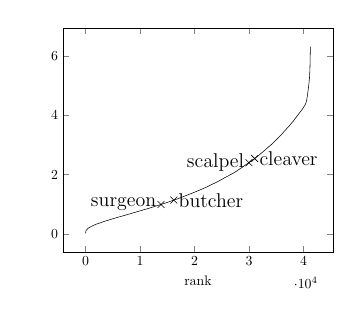
\begin{tikzpicture} [scale=0.5]
	\begin{axis} [xlabel=rank,ylabel=PMI,y label style={color=white}]
	\addplot [mark=none] coordinates {
(0,0.01004) (82,0.10112) (164,0.12417) (246,0.14062) (328,0.15755) (410,0.17296) (492,0.18456) (574,0.19468) (656,0.20589) (738,0.21453) (820,0.22473) (902,0.23274) (984,0.2401) (1066,0.24851) (1148,0.25546) (1230,0.26299) (1312,0.27054) (1394,0.27863) (1476,0.28481) (1558,0.2915) (1640,0.29752) (1722,0.30343) (1804,0.30956) (1886,0.31675) (1968,0.32333) (2050,0.32831) (2132,0.33313) (2214,0.3384) (2296,0.34394) (2378,0.34814) (2460,0.3538) (2542,0.35913) (2624,0.36444) (2706,0.36953) (2788,0.37487) (2870,0.37967) (2952,0.38513) (3034,0.38953) (3116,0.39547) (3198,0.40102) (3280,0.40585) (3362,0.41063) (3444,0.41565) (3526,0.42068) (3608,0.42616) (3690,0.4312) (3772,0.43623) (3854,0.44049) (3936,0.44462) (4018,0.44953) (4100,0.45438) (4182,0.45911) (4264,0.46431) (4346,0.46947) (4428,0.47387) (4510,0.47886) (4592,0.48422) (4674,0.48876) (4756,0.4925) (4838,0.49659) (4920,0.50107) (5002,0.50641) (5084,0.51135) (5166,0.51547) (5248,0.51932) (5330,0.52409) (5412,0.52829) (5494,0.53188) (5576,0.53712) (5658,0.5434) (5740,0.54751) (5822,0.55141) (5904,0.55585) (5986,0.56004) (6068,0.56406) (6150,0.56827) (6232,0.57183) (6314,0.57573) (6396,0.58003) (6478,0.58505) (6560,0.58909) (6642,0.5938) (6724,0.59793) (6806,0.60156) (6888,0.60534) (6970,0.61003) (7052,0.61445) (7134,0.61962) (7216,0.62455) (7298,0.62823) (7380,0.63238) (7462,0.63603) (7544,0.64026) (7626,0.64493) (7708,0.64952) (7790,0.65361) (7872,0.65815) (7954,0.66269) (8036,0.66683) (8118,0.67159) (8200,0.67607) (8282,0.67947) (8364,0.68488) (8446,0.68908) (8528,0.69304) (8610,0.69802) (8692,0.70339) (8774,0.70777) (8856,0.71124) (8938,0.71568) (9020,0.7198) (9102,0.7239) (9184,0.72878) (9266,0.73343) (9348,0.73723) (9430,0.74189) (9512,0.74635) (9594,0.75065) (9676,0.7557) (9758,0.75996) (9840,0.76391) (9922,0.76901) (10004,0.77353) (10086,0.77779) (10168,0.78219) (10250,0.78652) (10332,0.79145) (10414,0.79531) (10496,0.80012) (10578,0.80532) (10660,0.80945) (10742,0.81342) (10824,0.81732) (10906,0.82221) (10988,0.82745) (11070,0.83131) (11152,0.83563) (11234,0.83974) (11316,0.84422) (11398,0.84898) (11480,0.85286) (11562,0.85717) (11644,0.86237) (11726,0.86768) (11808,0.87183) (11890,0.8768) (11972,0.88124) (12054,0.88766) (12136,0.89174) (12218,0.89593) (12300,0.9004) (12382,0.90499) (12464,0.91022) (12546,0.91524) (12628,0.92063) (12710,0.92589) (12792,0.9302) (12874,0.93491) (12956,0.93958) (13038,0.94382) (13120,0.94897) (13202,0.95368) (13284,0.95825) (13366,0.96291) (13448,0.96773) (13530,0.97199) (13612,0.9763) (13694,0.98069) (13776,0.98459) (13858,0.98966) (13940,0.99399) (14022,0.99876) (14104,1.00333) (14186,1.00931) (14268,1.01341) (14350,1.01921) (14432,1.02376) (14514,1.02881) (14596,1.0337) (14678,1.03876) (14760,1.04444) (14842,1.04948) (14924,1.05469) (15006,1.05989) (15088,1.06474) (15170,1.06996) (15252,1.07588) (15334,1.08069) (15416,1.08643) (15498,1.09186) (15580,1.09734) (15662,1.10242) (15744,1.10785) (15826,1.11413) (15908,1.11883) (15990,1.1244) (16072,1.12913) (16154,1.13446) (16236,1.13927) (16318,1.14435) (16400,1.15018) (16482,1.15522) (16564,1.16049) (16646,1.16489) (16728,1.1701) (16810,1.17582) (16892,1.18192) (16974,1.18815) (17056,1.19322) (17138,1.19823) (17220,1.20358) (17302,1.20987) (17384,1.21516) (17466,1.21968) (17548,1.22499) (17630,1.23088) (17712,1.23803) (17794,1.24268) (17876,1.24986) (17958,1.25649) (18040,1.2622) (18122,1.26725) (18204,1.27383) (18286,1.28019) (18368,1.28526) (18450,1.29071) (18532,1.29788) (18614,1.30401) (18696,1.30931) (18778,1.31475) (18860,1.32057) (18942,1.32722) (19024,1.33404) (19106,1.33982) (19188,1.34682) (19270,1.3532) (19352,1.35828) (19434,1.36399) (19516,1.36963) (19598,1.37588) (19680,1.38155) (19762,1.38811) (19844,1.3934) (19926,1.39918) (20008,1.40595) (20090,1.41118) (20172,1.41886) (20254,1.42561) (20336,1.4322) (20418,1.43866) (20500,1.44371) (20582,1.44929) (20664,1.45499) (20746,1.46161) (20828,1.46834) (20910,1.47572) (20992,1.48208) (21074,1.48938) (21156,1.49567) (21238,1.502) (21320,1.50777) (21402,1.51482) (21484,1.52101) (21566,1.52692) (21648,1.53378) (21730,1.5405) (21812,1.54756) (21894,1.55427) (21976,1.56093) (22058,1.56736) (22140,1.57399) (22222,1.58047) (22304,1.58707) (22386,1.59404) (22468,1.60202) (22550,1.61023) (22632,1.61838) (22714,1.62572) (22796,1.63352) (22878,1.64017) (22960,1.6482) (23042,1.65694) (23124,1.66455) (23206,1.66957) (23288,1.67764) (23370,1.68445) (23452,1.69159) (23534,1.69743) (23616,1.7047) (23698,1.71182) (23780,1.71945) (23862,1.72803) (23944,1.73609) (24026,1.74283) (24108,1.74953) (24190,1.75746) (24272,1.76496) (24354,1.77295) (24436,1.7803) (24518,1.78909) (24600,1.79816) (24682,1.80732) (24764,1.81569) (24846,1.82402) (24928,1.83185) (25010,1.83983) (25092,1.84653) (25174,1.85539) (25256,1.86431) (25338,1.87298) (25420,1.88129) (25502,1.89292) (25584,1.90107) (25666,1.90717) (25748,1.91474) (25830,1.92326) (25912,1.93098) (25994,1.93822) (26076,1.94552) (26158,1.95458) (26240,1.96421) (26322,1.97138) (26404,1.98058) (26486,1.98953) (26568,1.99806) (26650,2.0048) (26732,2.01379) (26814,2.02163) (26896,2.03003) (26978,2.0378) (27060,2.04688) (27142,2.05528) (27224,2.06416) (27306,2.0726) (27388,2.08179) (27470,2.09186) (27552,2.1006) (27634,2.11046) (27716,2.11894) (27798,2.12917) (27880,2.14078) (27962,2.15169) (28044,2.16215) (28126,2.17069) (28208,2.18003) (28290,2.1901) (28372,2.20237) (28454,2.21281) (28536,2.22127) (28618,2.23267) (28700,2.24393) (28782,2.25311) (28864,2.26285) (28946,2.27433) (29028,2.28413) (29110,2.29509) (29192,2.30673) (29274,2.31722) (29356,2.3273) (29438,2.3381) (29520,2.34938) (29602,2.35963) (29684,2.36963) (29766,2.37996) (29848,2.38884) (29930,2.39786) (30012,2.40662) (30094,2.41785) (30176,2.42997) (30258,2.43904) (30340,2.44846) (30422,2.45941) (30504,2.47207) (30586,2.48308) (30668,2.49381) (30750,2.50379) (30832,2.51552) (30914,2.5269) (30996,2.53916) (31078,2.55115) (31160,2.56154) (31242,2.57291) (31324,2.58307) (31406,2.59604) (31488,2.60689) (31570,2.61998) (31652,2.63238) (31734,2.64579) (31816,2.65861) (31898,2.67144) (31980,2.68472) (32062,2.69803) (32144,2.712) (32226,2.72464) (32308,2.73657) (32390,2.74777) (32472,2.75953) (32554,2.77461) (32636,2.78639) (32718,2.79994) (32800,2.81118) (32882,2.82421) (32964,2.83656) (33046,2.84961) (33128,2.8645) (33210,2.87854) (33292,2.89033) (33374,2.90405) (33456,2.91733) (33538,2.92832) (33620,2.94034) (33702,2.95501) (33784,2.96828) (33866,2.98301) (33948,2.99515) (34030,3.00776) (34112,3.02234) (34194,3.03712) (34276,3.05141) (34358,3.06588) (34440,3.07913) (34522,3.09254) (34604,3.10971) (34686,3.12494) (34768,3.1389) (34850,3.15573) (34932,3.16772) (35014,3.17953) (35096,3.19689) (35178,3.20979) (35260,3.22681) (35342,3.24166) (35424,3.25793) (35506,3.27277) (35588,3.28864) (35670,3.30331) (35752,3.32018) (35834,3.33539) (35916,3.34992) (35998,3.36567) (36080,3.38042) (36162,3.39874) (36244,3.42298) (36326,3.43814) (36408,3.45543) (36490,3.472) (36572,3.48727) (36654,3.50482) (36736,3.5231) (36818,3.53751) (36900,3.55525) (36982,3.57058) (37064,3.58827) (37146,3.60348) (37228,3.6211) (37310,3.63785) (37392,3.6537) (37474,3.67321) (37556,3.69422) (37638,3.70843) (37720,3.72642) (37802,3.74467) (37884,3.76195) (37966,3.782) (38048,3.79854) (38130,3.81529) (38212,3.83622) (38294,3.85617) (38376,3.8778) (38458,3.89704) (38540,3.91657) (38622,3.93641) (38704,3.95512) (38786,3.97558) (38868,3.99189) (38950,4.01043) (39032,4.03438) (39114,4.05616) (39196,4.07354) (39278,4.09439) (39360,4.11559) (39442,4.13547) (39524,4.15566) (39606,4.17789) (39688,4.19701) (39770,4.21642) (39852,4.23612) (39934,4.25803) (40016,4.28428) (40098,4.31039) (40180,4.33158) (40262,4.35509) (40344,4.38619) (40426,4.42515) (40508,4.47456) (40590,4.55117) (40672,4.63453) (40754,4.74044) (40836,4.86945) (40918,4.977) (41000,5.1181) (41082,5.27117) (41164,5.55781) (41246,6.33026)
	};
	\addplot [mark=x,only marks,mark size = 3.5] coordinates {
		(13845,0.98899)(16190,1.13695)(29968,2.40174)(31024,2.54414)
	};
	\node [anchor=east] at (axis cs: 13845,0.98899) {\Large surgeon};
	\node [anchor=west] at (axis cs: 16190,1.13695) {\Large butcher};
	\node [anchor=east] at (axis cs: 29968,2.40174) {\Large scalpel};
	\node [anchor=west] at (axis cs: 31024,2.54414) {\Large cleaver};
	\end{axis}
\end{tikzpicture}
\caption*{dimension: \emph{hands}}
\end{subfigure}
\centering
\begin{subfigure} [t] {0.3 \textwidth}
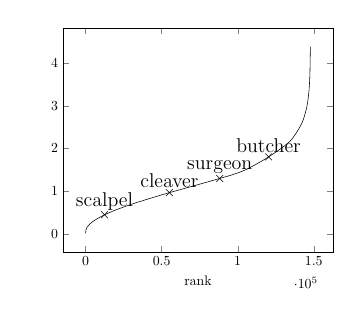
\begin{tikzpicture} [scale=0.5]
	\begin{axis} [xlabel=rank,ylabel=PMI,y label style={color=white}]
	\addplot [mark=none] coordinates {
		(0,0.00873) (295,0.08756) (590,0.12013) (885,0.14286) (1180,0.1607) (1475,0.17372) (1770,0.18662) (2065,0.20012) (2360,0.21206) (2655,0.22349) (2950,0.23441) (3245,0.24433) (3540,0.25194) (3835,0.26042) (4130,0.26934) (4425,0.27875) (4720,0.28699) (5015,0.29465) (5310,0.30183) (5605,0.30913) (5900,0.31561) (6195,0.32201) (6490,0.32861) (6785,0.33471) (7080,0.3407) (7375,0.3472) (7670,0.35305) (7965,0.35943) (8260,0.36555) (8555,0.37194) (8850,0.37792) (9145,0.38409) (9440,0.38982) (9735,0.39532) (10030,0.40097) (10325,0.4068) (10620,0.41244) (10915,0.4175) (11210,0.42332) (11505,0.4289) (11800,0.43381) (12095,0.43959) (12390,0.44398) (12685,0.44896) (12980,0.45406) (13275,0.45911) (13570,0.4639) (13865,0.46904) (14160,0.47337) (14455,0.47822) (14750,0.48215) (15045,0.48676) (15340,0.49105) (15635,0.4958) (15930,0.50037) (16225,0.50464) (16520,0.50927) (16815,0.51314) (17110,0.5178) (17405,0.5226) (17700,0.52745) (17995,0.53188) (18290,0.53667) (18585,0.54042) (18880,0.54459) (19175,0.54871) (19470,0.55311) (19765,0.55732) (20060,0.56142) (20355,0.56567) (20650,0.5698) (20945,0.57383) (21240,0.57791) (21535,0.58164) (21830,0.58552) (22125,0.58925) (22420,0.59313) (22715,0.59699) (23010,0.60082) (23305,0.60506) (23600,0.60903) (23895,0.61294) (24190,0.61639) (24485,0.62025) (24780,0.62395) (25075,0.62797) (25370,0.6315) (25665,0.63521) (25960,0.63898) (26255,0.64253) (26550,0.64675) (26845,0.65017) (27140,0.65398) (27435,0.65793) (27730,0.66142) (28025,0.66484) (28320,0.66857) (28615,0.67248) (28910,0.67612) (29205,0.67968) (29500,0.68328) (29795,0.68728) (30090,0.69088) (30385,0.69415) (30680,0.69775) (30975,0.70109) (31270,0.70435) (31565,0.70817) (31860,0.71161) (32155,0.71545) (32450,0.71891) (32745,0.72262) (33040,0.72637) (33335,0.72966) (33630,0.7331) (33925,0.73667) (34220,0.73973) (34515,0.74279) (34810,0.7459) (35105,0.74919) (35400,0.75252) (35695,0.75606) (35990,0.75912) (36285,0.76252) (36580,0.76565) (36875,0.76909) (37170,0.7723) (37465,0.77577) (37760,0.77899) (38055,0.78258) (38350,0.78613) (38645,0.78925) (38940,0.79236) (39235,0.79558) (39530,0.79895) (39825,0.80261) (40120,0.80618) (40415,0.8093) (40710,0.81259) (41005,0.81587) (41300,0.8189) (41595,0.822) (41890,0.82529) (42185,0.82836) (42480,0.831) (42775,0.8342) (43070,0.83738) (43365,0.84046) (43660,0.84368) (43955,0.84705) (44250,0.8503) (44545,0.8539) (44840,0.8571) (45135,0.86037) (45430,0.8634) (45725,0.86668) (46020,0.86967) (46315,0.87284) (46610,0.87596) (46905,0.87934) (47200,0.88226) (47495,0.88532) (47790,0.88815) (48085,0.89148) (48380,0.89464) (48675,0.89792) (48970,0.90121) (49265,0.90408) (49560,0.90712) (49855,0.9105) (50150,0.91355) (50445,0.91662) (50740,0.9196) (51035,0.92264) (51330,0.92587) (51625,0.92858) (51920,0.9317) (52215,0.93476) (52510,0.93752) (52805,0.94067) (53100,0.94403) (53395,0.94684) (53690,0.94973) (53985,0.9531) (54280,0.95608) (54575,0.95903) (54870,0.96235) (55165,0.96528) (55460,0.96823) (55755,0.9709) (56050,0.97389) (56345,0.97714) (56640,0.98012) (56935,0.98296) (57230,0.98571) (57525,0.98879) (57820,0.99174) (58115,0.99439) (58410,0.99753) (58705,1.00047) (59000,1.00323) (59295,1.00594) (59590,1.00932) (59885,1.01223) (60180,1.01548) (60475,1.01823) (60770,1.02118) (61065,1.02405) (61360,1.02711) (61655,1.03007) (61950,1.03277) (62245,1.03554) (62540,1.03864) (62835,1.04148) (63130,1.04441) (63425,1.04769) (63720,1.05068) (64015,1.05349) (64310,1.05632) (64605,1.05917) (64900,1.06239) (65195,1.06491) (65490,1.06798) (65785,1.071) (66080,1.07403) (66375,1.07658) (66670,1.07991) (66965,1.08284) (67260,1.08551) (67555,1.08852) (67850,1.09125) (68145,1.09441) (68440,1.09761) (68735,1.10049) (69030,1.10307) (69325,1.10642) (69620,1.10932) (69915,1.11248) (70210,1.11485) (70505,1.11804) (70800,1.12124) (71095,1.12447) (71390,1.12701) (71685,1.13009) (71980,1.13278) (72275,1.13605) (72570,1.13922) (72865,1.14204) (73160,1.14507) (73455,1.1477) (73750,1.15088) (74045,1.15353) (74340,1.15627) (74635,1.15954) (74930,1.16242) (75225,1.16531) (75520,1.16823) (75815,1.17134) (76110,1.17439) (76405,1.17706) (76700,1.18063) (76995,1.18332) (77290,1.18603) (77585,1.18921) (77880,1.19209) (78175,1.19502) (78470,1.19791) (78765,1.20069) (79060,1.20348) (79355,1.20629) (79650,1.20911) (79945,1.21241) (80240,1.21555) (80535,1.21861) (80830,1.22149) (81125,1.22487) (81420,1.22827) (81715,1.2312) (82010,1.23414) (82305,1.2371) (82600,1.24007) (82895,1.24306) (83190,1.24607) (83485,1.24909) (83780,1.25212) (84075,1.25535) (84370,1.25824) (84665,1.26133) (84960,1.26442) (85255,1.26754) (85550,1.27015) (85845,1.27382) (86140,1.27646) (86435,1.27964) (86730,1.28301) (87025,1.28595) (87320,1.28874) (87615,1.29198) (87910,1.29524) (88205,1.29761) (88500,1.30072) (88795,1.3032) (89090,1.30647) (89385,1.30959) (89680,1.31294) (89975,1.31632) (90270,1.31929) (90565,1.32248) (90860,1.32542) (91155,1.32867) (91450,1.3314) (91745,1.33452) (92040,1.33719) (92335,1.34049) (92630,1.34284) (92925,1.34614) (93220,1.34875) (93515,1.35203) (93810,1.35513) (94105,1.35834) (94400,1.36124) (94695,1.3644) (94990,1.36758) (95285,1.37061) (95580,1.37423) (95875,1.37795) (96170,1.38107) (96465,1.38484) (96760,1.38799) (97055,1.39179) (97350,1.3951) (97645,1.39904) (97940,1.40205) (98235,1.40594) (98530,1.40985) (98825,1.41309) (99120,1.41642) (99415,1.42032) (99710,1.4238) (100005,1.42707) (100300,1.43096) (100595,1.43467) (100890,1.4381) (101185,1.44215) (101480,1.44614) (101775,1.4503) (102070,1.45448) (102365,1.45869) (102660,1.46256) (102955,1.46711) (103250,1.47148) (103545,1.4758) (103840,1.48063) (104135,1.48506) (104430,1.4899) (104725,1.49483) (105020,1.4993) (105315,1.50405) (105610,1.50883) (105905,1.51364) (106200,1.51823) (106495,1.52355) (106790,1.52829) (107085,1.5334) (107380,1.53849) (107675,1.54404) (107970,1.54991) (108265,1.55528) (108560,1.56097) (108855,1.56671) (109150,1.57221) (109445,1.57817) (109740,1.58419) (110035,1.58962) (110330,1.59523) (110625,1.60124) (110920,1.60644) (111215,1.6124) (111510,1.61807) (111805,1.62349) (112100,1.62939) (112395,1.63614) (112690,1.64192) (112985,1.64777) (113280,1.65342) (113575,1.65958) (113870,1.6656) (114165,1.6715) (114460,1.67753) (114755,1.68362) (115050,1.69056) (115345,1.69642) (115640,1.70314) (115935,1.70894) (116230,1.71511) (116525,1.72116) (116820,1.72726) (117115,1.7334) (117410,1.7396) (117705,1.7455) (118000,1.75179) (118295,1.75814) (118590,1.76493) (118885,1.77188) (119180,1.77858) (119475,1.78441) (119770,1.79103) (120065,1.7977) (120360,1.8048) (120655,1.81196) (120950,1.81804) (121245,1.82571) (121540,1.83226) (121835,1.83877) (122130,1.84628) (122425,1.85314) (122720,1.85995) (123015,1.86691) (123310,1.87338) (123605,1.8807) (123900,1.88815) (124195,1.89467) (124490,1.90165) (124785,1.90879) (125080,1.91606) (125375,1.92384) (125670,1.93038) (125965,1.93784) (126260,1.94493) (126555,1.95164) (126850,1.95975) (127145,1.96748) (127440,1.97439) (127735,1.9813) (128030,1.98876) (128325,1.99629) (128620,2.00293) (128915,2.0101) (129210,2.0185) (129505,2.02609) (129800,2.0342) (130095,2.04288) (130390,2.05098) (130685,2.05863) (130980,2.06739) (131275,2.07588) (131570,2.08472) (131865,2.09207) (132160,2.10107) (132455,2.11016) (132750,2.11881) (133045,2.12863) (133340,2.13745) (133635,2.14679) (133930,2.15536) (134225,2.16597) (134520,2.17709) (134815,2.1879) (135110,2.20013) (135405,2.21217) (135700,2.22397) (135995,2.23776) (136290,2.25101) (136585,2.26502) (136880,2.28041) (137175,2.29604) (137470,2.3102) (137765,2.32542) (138060,2.3402) (138355,2.35664) (138650,2.37329) (138945,2.38835) (139240,2.40539) (139535,2.42262) (139830,2.43996) (140125,2.45796) (140420,2.47517) (140715,2.49428) (141010,2.51376) (141305,2.53363) (141600,2.55316) (141895,2.57224) (142190,2.59489) (142485,2.6199) (142780,2.6466) (143075,2.67209) (143370,2.70154) (143665,2.73407) (143960,2.77034) (144255,2.80907) (144550,2.84553) (144845,2.88325) (145140,2.92826) (145435,2.97315) (145730,3.03039) (146025,3.09462) (146320,3.17092) (146615,3.25689) (146910,3.36659) (147205,3.52351) (147500,3.75669) (147795,4.38804)
	};
	\addplot [mark=x,only marks,mark size = 3.5] coordinates {
		(12466,0.44529)(55096,0.9647)(88206,1.29763)(120293,1.80307)
	};
	\node [anchor=south] at (axis cs: 12466,0.44529) {\Large scalpel};
	\node [anchor=south] at (axis cs: 55096,0.9647) {\Large cleaver};
	\node [anchor=south] at (axis cs: 88206,1.29763) {\Large surgeon};
	\node [anchor=south] at (axis cs: 120293,1.80307) {\Large butcher};
	\end{axis}
\end{tikzpicture}
\caption*{dimension: \emph{known}}
\end{subfigure}
\caption{\textsc{surgery} $\Longleftrightarrow$ \textsc{butchery}}
\vspace{0.5cm}
\end{subfigure}
\begin{subfigure} {1 \textwidth}
\centering
\begin{subfigure} [t] {0.3 \textwidth}
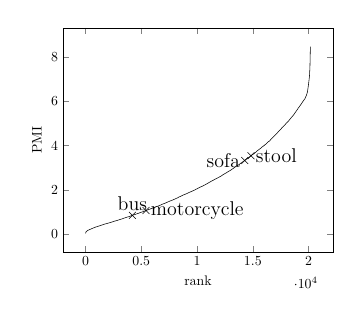
\begin{tikzpicture}[scale=0.5]
	\begin{axis} [xlabel=rank,ylabel=PMI]
	\addplot [mark=none] coordinates {
		(0,0.01807) (40,0.08801) (80,0.10418) (120,0.12301) (160,0.14129) (200,0.15581) (240,0.16573) (280,0.17348) (320,0.18302) (360,0.19209) (400,0.19925) (440,0.20666) (480,0.21617) (520,0.22443) (560,0.23427) (600,0.24492) (640,0.2522) (680,0.25943) (720,0.26829) (760,0.27649) (800,0.28612) (840,0.29261) (880,0.30053) (920,0.3083) (960,0.31429) (1000,0.32115) (1040,0.32744) (1080,0.33394) (1120,0.33954) (1160,0.34584) (1200,0.35315) (1240,0.36033) (1280,0.36684) (1320,0.37535) (1360,0.38349) (1400,0.38811) (1440,0.39368) (1480,0.40195) (1520,0.40817) (1560,0.41464) (1600,0.42235) (1640,0.42853) (1680,0.4332) (1720,0.43933) (1760,0.44643) (1800,0.45126) (1840,0.45798) (1880,0.46196) (1920,0.46764) (1960,0.47397) (2000,0.47976) (2040,0.48468) (2080,0.48959) (2120,0.49501) (2160,0.50245) (2200,0.50999) (2240,0.51565) (2280,0.52219) (2320,0.5278) (2360,0.53419) (2400,0.54039) (2440,0.54867) (2480,0.55612) (2520,0.56246) (2560,0.56867) (2600,0.57441) (2640,0.5796) (2680,0.58426) (2720,0.58904) (2760,0.59574) (2800,0.60044) (2840,0.60746) (2880,0.61395) (2920,0.62132) (2960,0.62723) (3000,0.63414) (3040,0.64035) (3080,0.64664) (3120,0.65309) (3160,0.65962) (3200,0.66545) (3240,0.67194) (3280,0.67898) (3320,0.68574) (3360,0.69314) (3400,0.70106) (3440,0.70755) (3480,0.71562) (3520,0.7207) (3560,0.72882) (3600,0.73589) (3640,0.74281) (3680,0.74879) (3720,0.7544) (3760,0.76031) (3800,0.76655) (3840,0.77243) (3880,0.77811) (3920,0.78593) (3960,0.79245) (4000,0.79987) (4040,0.80729) (4080,0.8142) (4120,0.82146) (4160,0.82796) (4200,0.83549) (4240,0.84197) (4280,0.84908) (4320,0.85632) (4360,0.86174) (4400,0.86933) (4440,0.8756) (4480,0.88284) (4520,0.89014) (4560,0.89881) (4600,0.90487) (4640,0.91227) (4680,0.91933) (4720,0.92417) (4760,0.93282) (4800,0.94148) (4840,0.94876) (4880,0.95675) (4920,0.96371) (4960,0.97209) (5000,0.97936) (5040,0.98524) (5080,0.99071) (5120,0.99736) (5160,1.00528) (5200,1.01284) (5240,1.02125) (5280,1.02867) (5320,1.03627) (5360,1.04287) (5400,1.05073) (5440,1.05861) (5480,1.06603) (5520,1.07379) (5560,1.08193) (5600,1.08765) (5640,1.09719) (5680,1.10606) (5720,1.11176) (5760,1.11926) (5800,1.12635) (5840,1.13377) (5880,1.14269) (5920,1.14935) (5960,1.15627) (6000,1.1636) (6040,1.1701) (6080,1.17731) (6120,1.18418) (6160,1.19197) (6200,1.1989) (6240,1.20822) (6280,1.21744) (6320,1.22496) (6360,1.23316) (6400,1.23927) (6440,1.24692) (6480,1.25445) (6520,1.26039) (6560,1.26904) (6600,1.27511) (6640,1.28492) (6680,1.29403) (6720,1.30086) (6760,1.31208) (6800,1.32188) (6840,1.32958) (6880,1.33859) (6920,1.34533) (6960,1.35409) (7000,1.36271) (7040,1.37123) (7080,1.37765) (7120,1.38479) (7160,1.39208) (7200,1.40575) (7240,1.41438) (7280,1.42119) (7320,1.43062) (7360,1.4395) (7400,1.44675) (7440,1.45623) (7480,1.46539) (7520,1.47414) (7560,1.48473) (7600,1.49235) (7640,1.49913) (7680,1.50652) (7720,1.51479) (7760,1.52353) (7800,1.53037) (7840,1.53949) (7880,1.54613) (7920,1.55628) (7960,1.56419) (8000,1.57432) (8040,1.58193) (8080,1.59268) (8120,1.60133) (8160,1.61242) (8200,1.61978) (8240,1.6293) (8280,1.63936) (8320,1.65024) (8360,1.66408) (8400,1.67438) (8440,1.68316) (8480,1.69048) (8520,1.69936) (8560,1.71055) (8600,1.72011) (8640,1.72834) (8680,1.73853) (8720,1.74845) (8760,1.76032) (8800,1.76736) (8840,1.7744) (8880,1.78424) (8920,1.79016) (8960,1.79683) (9000,1.80609) (9040,1.81228) (9080,1.82274) (9120,1.83172) (9160,1.8421) (9200,1.85209) (9240,1.86091) (9280,1.87269) (9320,1.88162) (9360,1.88979) (9400,1.89826) (9440,1.90599) (9480,1.91318) (9520,1.92505) (9560,1.93444) (9600,1.94571) (9640,1.95504) (9680,1.9624) (9720,1.97049) (9760,1.98027) (9800,1.98918) (9840,2.0016) (9880,2.00995) (9920,2.02339) (9960,2.03356) (10000,2.04012) (10040,2.05054) (10080,2.06164) (10120,2.07297) (10160,2.08342) (10200,2.0928) (10240,2.10547) (10280,2.11516) (10320,2.12376) (10360,2.13386) (10400,2.1439) (10440,2.15238) (10480,2.16081) (10520,2.17133) (10560,2.18265) (10600,2.19398) (10640,2.20381) (10680,2.21223) (10720,2.22306) (10760,2.23474) (10800,2.24643) (10840,2.25555) (10880,2.26544) (10920,2.27881) (10960,2.29083) (11000,2.30002) (11040,2.31485) (11080,2.32973) (11120,2.3392) (11160,2.3485) (11200,2.36166) (11240,2.37261) (11280,2.38412) (11320,2.39335) (11360,2.40443) (11400,2.41346) (11440,2.4227) (11480,2.43726) (11520,2.44936) (11560,2.45841) (11600,2.47049) (11640,2.48135) (11680,2.49211) (11720,2.50352) (11760,2.51282) (11800,2.52109) (11840,2.53395) (11880,2.545) (11920,2.55443) (11960,2.56242) (12000,2.57606) (12040,2.58694) (12080,2.59861) (12120,2.60894) (12160,2.61961) (12200,2.63369) (12240,2.64586) (12280,2.66221) (12320,2.67431) (12360,2.69066) (12400,2.6994) (12440,2.71171) (12480,2.72202) (12520,2.73614) (12560,2.74619) (12600,2.75654) (12640,2.76956) (12680,2.78287) (12720,2.79596) (12760,2.80968) (12800,2.81987) (12840,2.83228) (12880,2.84536) (12920,2.85678) (12960,2.86698) (13000,2.87818) (13040,2.89375) (13080,2.90522) (13120,2.92417) (13160,2.93753) (13200,2.94947) (13240,2.96012) (13280,2.97727) (13320,2.9919) (13360,3.00949) (13400,3.02117) (13440,3.03374) (13480,3.04755) (13520,3.05834) (13560,3.07082) (13600,3.0871) (13640,3.10039) (13680,3.10995) (13720,3.12238) (13760,3.13939) (13800,3.15244) (13840,3.16883) (13880,3.18291) (13920,3.20048) (13960,3.21259) (14000,3.22557) (14040,3.23974) (14080,3.25826) (14120,3.27274) (14160,3.28916) (14200,3.30187) (14240,3.31464) (14280,3.32685) (14320,3.34422) (14360,3.35955) (14400,3.37416) (14440,3.38942) (14480,3.40227) (14520,3.41754) (14560,3.43544) (14600,3.4499) (14640,3.46429) (14680,3.48082) (14720,3.49309) (14760,3.50882) (14800,3.52889) (14840,3.54133) (14880,3.55606) (14920,3.57191) (14960,3.58483) (15000,3.59644) (15040,3.6079) (15080,3.62025) (15120,3.63744) (15160,3.65677) (15200,3.67548) (15240,3.69116) (15280,3.7069) (15320,3.72407) (15360,3.74242) (15400,3.76264) (15440,3.77522) (15480,3.79392) (15520,3.80815) (15560,3.823) (15600,3.83745) (15640,3.85162) (15680,3.86861) (15720,3.88566) (15760,3.90269) (15800,3.92281) (15840,3.93808) (15880,3.95319) (15920,3.96735) (15960,3.98367) (16000,3.99655) (16040,4.01665) (16080,4.03154) (16120,4.04681) (16160,4.06307) (16200,4.08056) (16240,4.09747) (16280,4.11544) (16320,4.13794) (16360,4.16041) (16400,4.17619) (16440,4.18668) (16480,4.20069) (16520,4.21994) (16560,4.24088) (16600,4.27185) (16640,4.29437) (16680,4.31532) (16720,4.3308) (16760,4.35218) (16800,4.37409) (16840,4.39314) (16880,4.41213) (16920,4.43346) (16960,4.45623) (17000,4.47329) (17040,4.49395) (17080,4.5178) (17120,4.53568) (17160,4.55734) (17200,4.57458) (17240,4.59707) (17280,4.62703) (17320,4.64836) (17360,4.66724) (17400,4.68684) (17440,4.70584) (17480,4.72579) (17520,4.74673) (17560,4.77423) (17600,4.80443) (17640,4.82303) (17680,4.84336) (17720,4.86325) (17760,4.87968) (17800,4.89859) (17840,4.91932) (17880,4.93802) (17920,4.96176) (17960,4.98855) (18000,5.01136) (18040,5.03271) (18080,5.04927) (18120,5.06802) (18160,5.08802) (18200,5.11516) (18240,5.13573) (18280,5.16277) (18320,5.18799) (18360,5.21535) (18400,5.23597) (18440,5.26559) (18480,5.2857) (18520,5.31125) (18560,5.33205) (18600,5.35544) (18640,5.3811) (18680,5.40519) (18720,5.43988) (18760,5.46503) (18800,5.50009) (18840,5.52036) (18880,5.55379) (18920,5.58679) (18960,5.60966) (19000,5.63683) (19040,5.66454) (19080,5.70512) (19120,5.72745) (19160,5.75436) (19200,5.78418) (19240,5.81058) (19280,5.84203) (19320,5.86725) (19360,5.89922) (19400,5.92953) (19440,5.95886) (19480,5.99326) (19520,6.01635) (19560,6.04723) (19600,6.07737) (19640,6.09996) (19680,6.13968) (19720,6.17574) (19760,6.22564) (19800,6.27326) (19840,6.32788) (19880,6.40042) (19920,6.51553) (19960,6.64487) (20000,6.80067) (20040,6.97572) (20080,7.15608) (20120,7.55856) (20160,8.4825)
	};
	\addplot [mark=x,only marks,mark size = 3.5] coordinates {
		(4203,0.83647)(5424,1.05531)(14277,3.32574)(14839,3.5408)
	};
	\node [anchor=south] at (axis cs: 4203,0.83647) {\Large bus};
	\node [anchor=west] at (axis cs: 5424,1.05531) {\Large motorcycle};
	\node [anchor=east] at (axis cs: 14277,3.32574) {\Large sofa};
	\node [anchor=west] at (axis cs: 14839,3.5408) {\Large stool};
	\end{axis}
\end{tikzpicture}
\caption*{dimension: \emph{beneath}}
\end{subfigure}
\centering
\begin{subfigure} [t] {0.3 \textwidth}
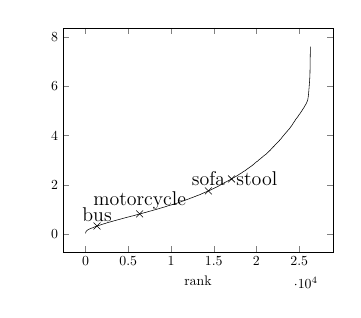
\begin{tikzpicture} [scale=0.5]
	\begin{axis} [xlabel=rank,ylabel=PMI,y label style={color=white}]
	\addplot [mark=none] coordinates {
(0,0.01675) (52,0.08641) (104,0.11395) (156,0.13152) (208,0.1449) (260,0.15729) (312,0.17009) (364,0.17929) (416,0.18943) (468,0.1969) (520,0.20568) (572,0.2132) (624,0.21885) (676,0.22786) (728,0.23473) (780,0.24152) (832,0.24796) (884,0.25543) (936,0.26243) (988,0.27045) (1040,0.27913) (1092,0.28643) (1144,0.29415) (1196,0.30079) (1248,0.30665) (1300,0.31381) (1352,0.31869) (1404,0.32553) (1456,0.32988) (1508,0.33585) (1560,0.34145) (1612,0.34818) (1664,0.35317) (1716,0.35886) (1768,0.36514) (1820,0.37003) (1872,0.37564) (1924,0.3832) (1976,0.39085) (2028,0.39488) (2080,0.4006) (2132,0.40667) (2184,0.41182) (2236,0.4179) (2288,0.42295) (2340,0.42819) (2392,0.43405) (2444,0.43963) (2496,0.44618) (2548,0.45159) (2600,0.45816) (2652,0.46318) (2704,0.46832) (2756,0.47341) (2808,0.47754) (2860,0.48276) (2912,0.48842) (2964,0.49329) (3016,0.49825) (3068,0.50391) (3120,0.50884) (3172,0.51291) (3224,0.5187) (3276,0.52385) (3328,0.52874) (3380,0.5338) (3432,0.53903) (3484,0.54366) (3536,0.54937) (3588,0.55397) (3640,0.55857) (3692,0.56373) (3744,0.56811) (3796,0.5727) (3848,0.57747) (3900,0.58307) (3952,0.5891) (4004,0.59307) (4056,0.59741) (4108,0.60246) (4160,0.60724) (4212,0.61081) (4264,0.61717) (4316,0.62245) (4368,0.62751) (4420,0.63213) (4472,0.63629) (4524,0.6414) (4576,0.64775) (4628,0.6524) (4680,0.65749) (4732,0.66224) (4784,0.66706) (4836,0.67126) (4888,0.67651) (4940,0.68154) (4992,0.68524) (5044,0.68999) (5096,0.69385) (5148,0.69916) (5200,0.70293) (5252,0.70693) (5304,0.71355) (5356,0.71872) (5408,0.72332) (5460,0.72674) (5512,0.73123) (5564,0.73429) (5616,0.73977) (5668,0.74452) (5720,0.75034) (5772,0.75588) (5824,0.76084) (5876,0.76676) (5928,0.7713) (5980,0.77605) (6032,0.78111) (6084,0.78565) (6136,0.79083) (6188,0.79523) (6240,0.80015) (6292,0.8061) (6344,0.81023) (6396,0.81556) (6448,0.81937) (6500,0.82353) (6552,0.82768) (6604,0.83212) (6656,0.83751) (6708,0.84267) (6760,0.84799) (6812,0.85396) (6864,0.85863) (6916,0.86424) (6968,0.86889) (7020,0.8725) (7072,0.87776) (7124,0.88178) (7176,0.88732) (7228,0.89208) (7280,0.89809) (7332,0.90496) (7384,0.90931) (7436,0.91509) (7488,0.91987) (7540,0.92362) (7592,0.92844) (7644,0.93292) (7696,0.93776) (7748,0.94194) (7800,0.94755) (7852,0.95238) (7904,0.95773) (7956,0.96306) (8008,0.97007) (8060,0.97382) (8112,0.97951) (8164,0.98387) (8216,0.98935) (8268,0.99435) (8320,0.9995) (8372,1.00407) (8424,1.00961) (8476,1.01384) (8528,1.02025) (8580,1.02592) (8632,1.03259) (8684,1.03735) (8736,1.0435) (8788,1.0487) (8840,1.05465) (8892,1.06012) (8944,1.06401) (8996,1.07007) (9048,1.07441) (9100,1.07969) (9152,1.0847) (9204,1.09) (9256,1.09604) (9308,1.10209) (9360,1.10758) (9412,1.11374) (9464,1.11928) (9516,1.12455) (9568,1.13098) (9620,1.13692) (9672,1.14262) (9724,1.14858) (9776,1.1536) (9828,1.15842) (9880,1.16313) (9932,1.16853) (9984,1.17291) (10036,1.17854) (10088,1.18346) (10140,1.18852) (10192,1.19436) (10244,1.199) (10296,1.20414) (10348,1.20985) (10400,1.21496) (10452,1.22073) (10504,1.22604) (10556,1.23157) (10608,1.23724) (10660,1.24303) (10712,1.2509) (10764,1.25676) (10816,1.26352) (10868,1.26996) (10920,1.27608) (10972,1.28217) (11024,1.28931) (11076,1.2969) (11128,1.30266) (11180,1.30913) (11232,1.31495) (11284,1.3221) (11336,1.32859) (11388,1.33513) (11440,1.33995) (11492,1.34681) (11544,1.35484) (11596,1.36172) (11648,1.3687) (11700,1.37499) (11752,1.38126) (11804,1.38807) (11856,1.39423) (11908,1.40122) (11960,1.40758) (12012,1.41314) (12064,1.41881) (12116,1.42723) (12168,1.43483) (12220,1.4424) (12272,1.45004) (12324,1.45626) (12376,1.46225) (12428,1.46947) (12480,1.47682) (12532,1.48399) (12584,1.49058) (12636,1.49646) (12688,1.50401) (12740,1.51107) (12792,1.51755) (12844,1.52406) (12896,1.53161) (12948,1.54055) (13000,1.54726) (13052,1.55481) (13104,1.56229) (13156,1.56842) (13208,1.57561) (13260,1.58041) (13312,1.58707) (13364,1.59383) (13416,1.60063) (13468,1.60916) (13520,1.61841) (13572,1.62766) (13624,1.63437) (13676,1.64123) (13728,1.64889) (13780,1.65654) (13832,1.66581) (13884,1.67465) (13936,1.68224) (13988,1.68884) (14040,1.6962) (14092,1.70327) (14144,1.71105) (14196,1.71988) (14248,1.72675) (14300,1.73522) (14352,1.74508) (14404,1.75366) (14456,1.76129) (14508,1.76854) (14560,1.77598) (14612,1.78352) (14664,1.79208) (14716,1.79963) (14768,1.81081) (14820,1.81956) (14872,1.82727) (14924,1.83641) (14976,1.84516) (15028,1.85275) (15080,1.86176) (15132,1.87215) (15184,1.88023) (15236,1.8889) (15288,1.89521) (15340,1.90477) (15392,1.91482) (15444,1.92311) (15496,1.93267) (15548,1.94245) (15600,1.95205) (15652,1.96163) (15704,1.97043) (15756,1.98125) (15808,1.99479) (15860,2.00513) (15912,2.01522) (15964,2.02509) (16016,2.03434) (16068,2.04523) (16120,2.05538) (16172,2.06331) (16224,2.0722) (16276,2.08273) (16328,2.09225) (16380,2.1047) (16432,2.11348) (16484,2.12113) (16536,2.13223) (16588,2.14104) (16640,2.15074) (16692,2.15914) (16744,2.16867) (16796,2.17831) (16848,2.18905) (16900,2.19981) (16952,2.20986) (17004,2.22016) (17056,2.22952) (17108,2.24112) (17160,2.2524) (17212,2.26303) (17264,2.27275) (17316,2.28305) (17368,2.29236) (17420,2.30235) (17472,2.31389) (17524,2.32247) (17576,2.33377) (17628,2.34477) (17680,2.35246) (17732,2.36392) (17784,2.37516) (17836,2.38815) (17888,2.40185) (17940,2.41244) (17992,2.42555) (18044,2.43546) (18096,2.44603) (18148,2.45423) (18200,2.46665) (18252,2.47727) (18304,2.48994) (18356,2.50535) (18408,2.51738) (18460,2.53018) (18512,2.53968) (18564,2.55015) (18616,2.56066) (18668,2.5726) (18720,2.58505) (18772,2.60085) (18824,2.6142) (18876,2.6275) (18928,2.64396) (18980,2.65579) (19032,2.66746) (19084,2.67906) (19136,2.69355) (19188,2.70469) (19240,2.71982) (19292,2.73115) (19344,2.74121) (19396,2.75699) (19448,2.77041) (19500,2.78374) (19552,2.79891) (19604,2.81135) (19656,2.82638) (19708,2.84447) (19760,2.85752) (19812,2.8759) (19864,2.88972) (19916,2.90431) (19968,2.92158) (20020,2.93576) (20072,2.94642) (20124,2.95941) (20176,2.9784) (20228,2.99452) (20280,3.01251) (20332,3.02487) (20384,3.03804) (20436,3.05077) (20488,3.06348) (20540,3.07917) (20592,3.09429) (20644,3.11226) (20696,3.12684) (20748,3.14204) (20800,3.15915) (20852,3.17397) (20904,3.18936) (20956,3.20496) (21008,3.21419) (21060,3.22974) (21112,3.24272) (21164,3.25946) (21216,3.27766) (21268,3.29491) (21320,3.30948) (21372,3.32466) (21424,3.34304) (21476,3.3615) (21528,3.37847) (21580,3.39682) (21632,3.41088) (21684,3.43391) (21736,3.4536) (21788,3.47507) (21840,3.49741) (21892,3.51271) (21944,3.53374) (21996,3.55207) (22048,3.56778) (22100,3.58534) (22152,3.60822) (22204,3.62608) (22256,3.64474) (22308,3.66202) (22360,3.68049) (22412,3.70251) (22464,3.71827) (22516,3.7392) (22568,3.75522) (22620,3.77581) (22672,3.79518) (22724,3.81597) (22776,3.84035) (22828,3.85796) (22880,3.87493) (22932,3.89799) (22984,3.92195) (23036,3.94708) (23088,3.96697) (23140,3.99179) (23192,4.0129) (23244,4.03537) (23296,4.0567) (23348,4.07813) (23400,4.09808) (23452,4.11888) (23504,4.13838) (23556,4.15818) (23608,4.17914) (23660,4.20302) (23712,4.22209) (23764,4.24442) (23816,4.26562) (23868,4.28565) (23920,4.31066) (23972,4.33902) (24024,4.36021) (24076,4.38092) (24128,4.40898) (24180,4.43671) (24232,4.46849) (24284,4.4919) (24336,4.52231) (24388,4.55091) (24440,4.57727) (24492,4.60037) (24544,4.62626) (24596,4.66056) (24648,4.68084) (24700,4.70331) (24752,4.73129) (24804,4.75594) (24856,4.77839) (24908,4.80801) (24960,4.8369) (25012,4.85793) (25064,4.88216) (25116,4.90684) (25168,4.93197) (25220,4.96521) (25272,4.98949) (25324,5.01507) (25376,5.04718) (25428,5.07343) (25480,5.10189) (25532,5.12923) (25584,5.15713) (25636,5.19463) (25688,5.21875) (25740,5.25195) (25792,5.2825) (25844,5.31375) (25896,5.35893) (25948,5.40143) (26000,5.4551) (26052,5.55495) (26104,5.72367) (26156,5.93883) (26208,6.16748) (26260,6.45446) (26312,7.62282)
	};
	\addplot [mark=x,only marks,mark size = 3.5] coordinates {
		(1347,0.3181)(6330,0.80923)(14379,1.74923)(17088,2.23614)
	};
	\node [anchor=south] at (axis cs: 1347,0.3181) {\Large bus};
	\node [anchor=south] at (axis cs: 6330,0.80923) {\Large motorcycle};
	\node [anchor=south] at (axis cs: 14379,1.74923) {\Large sofa};
	\node [anchor=west] at (axis cs: 17088,2.23614) {\Large stool};
	\end{axis}
\end{tikzpicture}
\caption*{dimension: \emph{hearing}}
\end{subfigure}
\centering
\begin{subfigure} [t] {0.3 \textwidth}
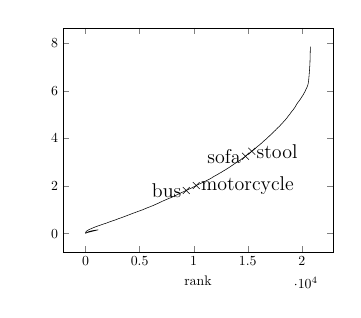
\begin{tikzpicture} [scale=0.5]
	\begin{axis} [xlabel=rank,ylabel=PMI,y label style={color=white}]
	\addplot [mark=none] coordinates {
		(0,0.00873) (295,0.08756) (590,0.12013) (885,0.14286) (1180,0.1607) (0,0.02677) (41,0.08065) (82,0.09906) (123,0.11429) (164,0.12671) (205,0.13769) (246,0.15083) (287,0.15995) (328,0.1692) (369,0.17824) (410,0.18709) (451,0.1952) (492,0.20434) (533,0.21495) (574,0.22229) (615,0.231) (656,0.23651) (697,0.24479) (738,0.25062) (779,0.25834) (820,0.26579) (861,0.27467) (902,0.28138) (943,0.28992) (984,0.29536) (1025,0.30141) (1066,0.30805) (1107,0.31515) (1148,0.3234) (1189,0.33087) (1230,0.33604) (1271,0.34317) (1312,0.34886) (1353,0.35541) (1394,0.36184) (1435,0.36848) (1476,0.37429) (1517,0.3822) (1558,0.38764) (1599,0.39293) (1640,0.40098) (1681,0.40823) (1722,0.41419) (1763,0.41853) (1804,0.42409) (1845,0.43063) (1886,0.43627) (1927,0.4425) (1968,0.44997) (2009,0.45531) (2050,0.46365) (2091,0.47124) (2132,0.47824) (2173,0.48498) (2214,0.49143) (2255,0.49638) (2296,0.50453) (2337,0.50989) (2378,0.51776) (2419,0.52444) (2460,0.53138) (2501,0.53735) (2542,0.54366) (2583,0.54887) (2624,0.55373) (2665,0.56101) (2706,0.56837) (2747,0.57471) (2788,0.58221) (2829,0.58937) (2870,0.59654) (2911,0.6041) (2952,0.61068) (2993,0.61865) (3034,0.62573) (3075,0.63437) (3116,0.64067) (3157,0.6466) (3198,0.65201) (3239,0.65797) (3280,0.6627) (3321,0.67009) (3362,0.67685) (3403,0.68503) (3444,0.69181) (3485,0.69843) (3526,0.706) (3567,0.71317) (3608,0.71995) (3649,0.72626) (3690,0.73292) (3731,0.73845) (3772,0.74578) (3813,0.75459) (3854,0.76254) (3895,0.76946) (3936,0.77635) (3977,0.78266) (4018,0.7903) (4059,0.7962) (4100,0.80308) (4141,0.81333) (4182,0.81938) (4223,0.82798) (4264,0.83336) (4305,0.83946) (4346,0.8467) (4387,0.85462) (4428,0.86113) (4469,0.86697) (4510,0.87293) (4551,0.88068) (4592,0.88904) (4633,0.89612) (4674,0.90291) (4715,0.90854) (4756,0.91565) (4797,0.923) (4838,0.92996) (4879,0.93744) (4920,0.94498) (4961,0.95142) (5002,0.95665) (5043,0.96379) (5084,0.97191) (5125,0.97696) (5166,0.98439) (5207,0.99203) (5248,0.99845) (5289,1.00495) (5330,1.01449) (5371,1.02037) (5412,1.02965) (5453,1.03662) (5494,1.04487) (5535,1.05414) (5576,1.06264) (5617,1.06717) (5658,1.07636) (5699,1.0831) (5740,1.0914) (5781,1.09796) (5822,1.10442) (5863,1.11144) (5904,1.11903) (5945,1.12612) (5986,1.13425) (6027,1.14157) (6068,1.14735) (6109,1.15481) (6150,1.16252) (6191,1.17077) (6232,1.17669) (6273,1.18503) (6314,1.19393) (6355,1.203) (6396,1.21346) (6437,1.22099) (6478,1.22696) (6519,1.2346) (6560,1.2437) (6601,1.25364) (6642,1.26292) (6683,1.26935) (6724,1.27874) (6765,1.28735) (6806,1.29474) (6847,1.30644) (6888,1.31405) (6929,1.32195) (6970,1.33023) (7011,1.33851) (7052,1.34919) (7093,1.35808) (7134,1.36713) (7175,1.3762) (7216,1.38341) (7257,1.39165) (7298,1.39816) (7339,1.40533) (7380,1.41374) (7421,1.42319) (7462,1.4328) (7503,1.43961) (7544,1.4477) (7585,1.45504) (7626,1.46103) (7667,1.4698) (7708,1.47748) (7749,1.487) (7790,1.49331) (7831,1.5012) (7872,1.50807) (7913,1.517) (7954,1.52501) (7995,1.53592) (8036,1.54448) (8077,1.55541) (8118,1.56479) (8159,1.57164) (8200,1.57983) (8241,1.58766) (8282,1.59751) (8323,1.60662) (8364,1.61387) (8405,1.62224) (8446,1.63037) (8487,1.63835) (8528,1.64723) (8569,1.658) (8610,1.66551) (8651,1.67428) (8692,1.68384) (8733,1.69278) (8774,1.70178) (8815,1.70988) (8856,1.71869) (8897,1.72736) (8938,1.73621) (8979,1.74417) (9020,1.75178) (9061,1.76248) (9102,1.76954) (9143,1.77959) (9184,1.78967) (9225,1.79854) (9266,1.80531) (9307,1.81463) (9348,1.82364) (9389,1.82984) (9430,1.83987) (9471,1.84816) (9512,1.85831) (9553,1.86775) (9594,1.87574) (9635,1.88361) (9676,1.89195) (9717,1.90189) (9758,1.90895) (9799,1.9185) (9840,1.9287) (9881,1.93976) (9922,1.94862) (9963,1.95758) (10004,1.96519) (10045,1.97336) (10086,1.98349) (10127,1.99438) (10168,2.00195) (10209,2.01153) (10250,2.02289) (10291,2.03234) (10332,2.04407) (10373,2.05289) (10414,2.06208) (10455,2.072) (10496,2.07941) (10537,2.0881) (10578,2.0964) (10619,2.10572) (10660,2.1147) (10701,2.12445) (10742,2.13346) (10783,2.14143) (10824,2.15069) (10865,2.15857) (10906,2.16899) (10947,2.17834) (10988,2.18676) (11029,2.19426) (11070,2.2011) (11111,2.20938) (11152,2.2209) (11193,2.22953) (11234,2.2379) (11275,2.24709) (11316,2.2573) (11357,2.26566) (11398,2.27685) (11439,2.28614) (11480,2.29569) (11521,2.30613) (11562,2.32011) (11603,2.32923) (11644,2.33655) (11685,2.34803) (11726,2.36436) (11767,2.3754) (11808,2.38662) (11849,2.39789) (11890,2.40615) (11931,2.41724) (11972,2.42661) (12013,2.43427) (12054,2.44468) (12095,2.45797) (12136,2.46996) (12177,2.47963) (12218,2.49114) (12259,2.49949) (12300,2.51444) (12341,2.52486) (12382,2.53655) (12423,2.54673) (12464,2.55574) (12505,2.5651) (12546,2.57442) (12587,2.58626) (12628,2.60064) (12669,2.61123) (12710,2.62377) (12751,2.63353) (12792,2.64563) (12833,2.65457) (12874,2.66541) (12915,2.67736) (12956,2.68664) (12997,2.69762) (13038,2.71349) (13079,2.72282) (13120,2.73751) (13161,2.75075) (13202,2.7607) (13243,2.76973) (13284,2.78335) (13325,2.79489) (13366,2.8062) (13407,2.81788) (13448,2.8316) (13489,2.84773) (13530,2.85953) (13571,2.86984) (13612,2.8832) (13653,2.89679) (13694,2.90957) (13735,2.92336) (13776,2.93424) (13817,2.94975) (13858,2.9605) (13899,2.97309) (13940,2.98267) (13981,2.99356) (14022,3.00853) (14063,3.01883) (14104,3.0299) (14145,3.04079) (14186,3.05526) (14227,3.06651) (14268,3.07863) (14309,3.09185) (14350,3.10502) (14391,3.1221) (14432,3.13603) (14473,3.15094) (14514,3.16297) (14555,3.17606) (14596,3.18689) (14637,3.19835) (14678,3.21075) (14719,3.22322) (14760,3.23922) (14801,3.25864) (14842,3.27703) (14883,3.28839) (14924,3.30348) (14965,3.31775) (15006,3.33425) (15047,3.34785) (15088,3.36307) (15129,3.37775) (15170,3.39287) (15211,3.4054) (15252,3.41985) (15293,3.4337) (15334,3.45112) (15375,3.46468) (15416,3.47705) (15457,3.49023) (15498,3.50164) (15539,3.52021) (15580,3.53471) (15621,3.5474) (15662,3.56152) (15703,3.57749) (15744,3.59924) (15785,3.6151) (15826,3.63472) (15867,3.65022) (15908,3.66346) (15949,3.68041) (15990,3.69407) (16031,3.70741) (16072,3.72448) (16113,3.73897) (16154,3.75398) (16195,3.77122) (16236,3.78797) (16277,3.80516) (16318,3.82257) (16359,3.84033) (16400,3.85569) (16441,3.87244) (16482,3.88989) (16523,3.90796) (16564,3.92399) (16605,3.94061) (16646,3.95372) (16687,3.96735) (16728,3.98657) (16769,4.00568) (16810,4.02217) (16851,4.04267) (16892,4.05943) (16933,4.07469) (16974,4.09078) (17015,4.11304) (17056,4.12674) (17097,4.14625) (17138,4.16004) (17179,4.17935) (17220,4.19326) (17261,4.21285) (17302,4.23273) (17343,4.24945) (17384,4.26941) (17425,4.29428) (17466,4.31052) (17507,4.32539) (17548,4.34017) (17589,4.35995) (17630,4.38333) (17671,4.40323) (17712,4.41498) (17753,4.43752) (17794,4.45723) (17835,4.4727) (17876,4.48776) (17917,4.50509) (17958,4.52632) (17999,4.54728) (18040,4.56731) (18081,4.58637) (18122,4.6068) (18163,4.62796) (18204,4.64858) (18245,4.66817) (18286,4.69012) (18327,4.71104) (18368,4.73228) (18409,4.7488) (18450,4.76772) (18491,4.79213) (18532,4.81396) (18573,4.83353) (18614,4.85713) (18655,4.88483) (18696,4.91393) (18737,4.9368) (18778,4.95964) (18819,4.98094) (18860,5.00694) (18901,5.02989) (18942,5.06233) (18983,5.08253) (19024,5.10587) (19065,5.12961) (19106,5.1567) (19147,5.17936) (19188,5.1987) (19229,5.22071) (19270,5.25074) (19311,5.27716) (19352,5.30173) (19393,5.33715) (19434,5.36873) (19475,5.40175) (19516,5.43814) (19557,5.4595) (19598,5.48969) (19639,5.51546) (19680,5.53591) (19721,5.55929) (19762,5.58441) (19803,5.61271) (19844,5.63882) (19885,5.66969) (19926,5.6969) (19967,5.72762) (20008,5.7545) (20049,5.77884) (20090,5.81302) (20131,5.83841) (20172,5.87575) (20213,5.91056) (20254,5.93799) (20295,5.97812) (20336,6.0231) (20377,6.06203) (20418,6.09435) (20459,6.13534) (20500,6.18576) (20541,6.22955) (20582,6.29717) (20623,6.421) (20664,6.62848) (20705,6.86175) (20746,7.13908) (20787,7.85674)
	};
	\addplot [mark=x,only marks,mark size = 3.5] coordinates {
		(9312,1.81529)(10235,2.01808)(14787,3.24988)(15370,3.46375)
	};
	\node [anchor=east] at (axis cs: 9312,1.81529) {\Large bus};
	\node [anchor=west] at (axis cs: 10235,2.01808) {\Large motorcycle};
	\node [anchor=east] at (axis cs: 14787,3.24988) {\Large sofa};
	\node [anchor=west] at (axis cs: 15370,3.46375) {\Large stool};
	\end{axis}
\end{tikzpicture}
\caption*{dimension: \emph{accidentally}}
\end{subfigure}
\caption{\textsc{furniture} $\Longleftrightarrow$ \textsc{vehicles}}
\end{subfigure}
\caption[The Arithmetic of Analogy]{Histograms of the top three co-occurrence dimensions satisfying the expected arithmetic of two analogies.}
\label{fig:histograms}
\end{figure}

What stands out here is the way that the analogical word-vectors tend to cluster into pairs.  This makes sense, since the formula described above indicates instances where the relationship between two of the word vectors is very similar to the relationship between the other two: this requirement is nicely satisfied by pairing word-vectors up with one another.  These dimensional values are pushed into two-dimensional projections of three-dimensional spaces in Figure~\ref{fig:inspace}, and here the well-defined parallelograms expected from this method of dimension selection become apparent.  In fact, more than just parallelograms, the shapes that begin to emerge are specifically rectangular in nature.  If we imagine extending the process of selecting dimensions where target word-vectors are clustered into pairs into higher dimensional subspaces, we can see that the vertices of the shapes that would evolve would tend towards right angles, and so this indicates an additional geometric feature of the relationships between lexical semantic representations that we might associate with analogy.

\revJB{6}{It must additionally be noted that the dimensions revealed as best suited for these analogies are not necessarily associated with co-occurrences that correspond to the conceptual basis of the analogies in any obvious way.  Returning to a point made in Chapter~\ref{sec:project}, the labels of co-occurrence dimensions associated with a given input may not reveal an immediately intuitive conceptual connection, though there will always be an opportunity for recourse to actual observations in the underlying corpus that will at least corroborate the statistical foundations of a contextualised analogy.    Furthermore, again as seen in the examples provided in Chapter~\ref{sec:project}, a more coherent profile of co-occurrence features is likely to emerge as we move into higher dimensional spaces

Our first task is to find amongst this profile of relevant co-occurrences those dimensions which are particularly suited to completing an analogy in a prescribed way, and so the objective will be to discover, not to interpret, these analogically efficacious dimensions.  An exploration of more sophisticated techniques for selecting these dimensions will be discussed at the end of this chapter, but the application and subsequent of, for instance, machine learning techniques for learning a methodology for reliably specifying analogical subspaces will ultimately be left for the future.}

Another interesting thing to note about the configurations in Figure~\ref{fig:inspace} is the oblong nature of the shapes.  In fact, it seems as though the word-vectors are orientating themselves in terms of types---though not necessarily in alignment with the conceptual categories we presumed to delineate the analogical mappings.  So, where \emph{bus} and \emph{motorcycle} might be seen as occupying a \textsc{vehicle} extent of the subspace as opposed to the \textsc{furniture} region inhabited by \emph{sofa} and \emph{stool}, \emph{surgeon} and \emph{butcher} seem to be establishing a region of \textsc{professions} while \emph{scalpel} and \emph{cleaver} could be construed in a domain of \textsc{implements}.  These distinctions are, naturally, a peculiarity of the dimensions themselves, with \emph{hands} in particular specifying a high co-occurrence with \textsc{implements}, while the preposition \emph{beneath}, with its spatial intimations, remits high values for \emph{sofa} and \emph{stool} (denotations of things that other things can be beneath); the prevalence of these same terms in co-occurrences with \emph{hearing} is less obvious but nonetheless indicative.

\begin{figure}
\centering
\begin{subfigure} [t] {0.45\textwidth}
\centering
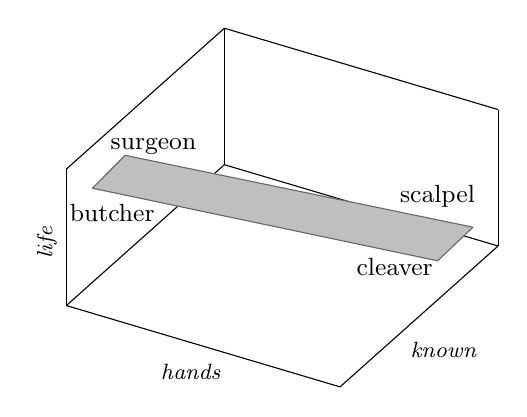
\begin{tikzpicture}
%\begin{axis}[view={120}{10},xmin=0,xmax=4.5,ymin=0,ymax=4.5,zmin=0,zmax=4.5,xlabel=gray,ylabel=relate, zlabel=tone,colormap/blackwhite]
\begin{axis}[view={120}{50},scale = 0.8,xlabel=\footnotesize\emph{known},ylabel=\footnotesize\emph{hands},zlabel=\footnotesize\emph{life},ticks=none,colormap/blackwhite]
%\addplot3 [color=black,->,ultra thick] coordinates {(0,0,0) (4,4,4)};
\addplot3[patch,patch type=rectangle,color=lightgray,fill opacity=1] coordinates {
 	(0.44529,2.40174,0.70908) (0.9647,2.54414,0.77903) (1.80307,1.13695,0.99632) (1.2979763,0.98899,0.92747)
};
\node [anchor=south] at (axis cs: 0.44529,2.2,0.70908) {\small scalpel};
\node [anchor=north] at (axis cs: 0.9647,2.3,0.77903) {\small cleaver};
\node [anchor=south] at (axis cs: 1.2979763,1.15,0.92747) {\small surgeon};
\node [anchor=north] at (axis cs: 1.80307,1.25,0.99632) {\small butcher};
%\addplot3 [color=black,->,ultra thick] coordinates {(2.2,2.2,2.2) (4,4,4)};
\end{axis}
\end{tikzpicture}
\caption{\textsc{surgery} $\Longleftrightarrow$ \textsc{butchery}}
\label{FIG:subspace}
\end{subfigure}
\hspace{0.05\textwidth}
\begin{subfigure} [t] {0.45\textwidth}
\centering
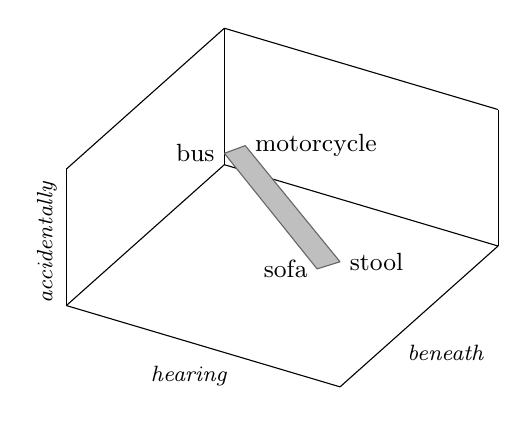
\begin{tikzpicture}
%\begin{axis}[view={120}{10},xmin=0,xmax=4.5,ymin=0,ymax=4.5,zmin=0,zmax=4.5,xlabel=gray,ylabel=relate, zlabel=tone,colormap/blackwhite]
\begin{axis}[view={120}{50},scale=0.8,xlabel=\footnotesize\emph{beneath},ylabel=\footnotesize\emph{hearing}, zlabel=\footnotesize\emph{accidentally},ticks=none, colormap/blackwhite]
%\addplot3 [color=black,->,ultra thick] coordinates {(0,0,0) (4,4,4)};
\addplot3[patch,patch type=rectangle,color=lightgray,fill opacity=1] coordinates {
 	(0.83647,1.81529,0.3181) (1.05531,2.01808,0.80923) (3.5408,3.46375,2.23614) (3.32574,3.24988,1.74923)
};
\node [anchor=east] at (axis cs: 0.83647,1.81529,0.3181) {\small bus};
\node [anchor=west] at (axis cs: 1.05531,2.01808,0.80923) {\small motorcycle};
\node [anchor=east] at (axis cs: 3.32574,3.24988,1.74923) {\small sofa};
\node [anchor=west] at (axis cs: 3.5408,3.46375,2.23614) {\small stool};
%\addplot3 [color=black,->,ultra thick] coordinates {(2.2,2.2,2.2) (4,4,4)};
\end{axis}
\end{tikzpicture}
\caption{\textsc{furniture} $\Longleftrightarrow$ \textsc{vehicles}}
\end{subfigure}
\caption[Two Analogies in Space]{The geometry of two analogies projected into subspaces defined by the three most analogically accurate dimensions.}
\label{fig:inspace}
\end{figure}

One of the things to take away from this small-scale qualitative analysis is that, at the end of the day, any four-point analogy can be cut along at least two different conceptual axes, corresponding to the intensions that semantically bind the representations along each edge of the rectangle.  We might easily speculate that the shapes found in well-formed analogical subspaces will be elongated along the axes that correspond to what humans might tend to classify as the conceptually salient distinction inherent in the analogy, but there are presumably also a variety of ways to make an orthogonal distinction, and we can reasonably expect these secondary characteristics of the analogical relationship to emerge in higher dimensional spaces.  In fact, a reasonable hypothesis, raised in \cite{McGregorEA2016}, is that contextualised analogical planes should, as dimensionality increases, begin to assume a more sqaure shape and a more central position in a subspace.

So I think it makes sense to expand this approach to analogy modelling to cover more analogies, and to examine the way that higher dimensionalities provide a basis for geometric analysis.  In order to efficiently and systematically test the viability of context sensitive subspaces for analogy solution, I randomly select a subset of 996 analogies from the data, described above, designed by \cite{MikolovEA2013b}, and project 400 dimensional subspaces from both 2x2 and 5x5 word window base spaces using the \textsc{joint}, \textsc{indy}, and \textsc{zipped} techniques, taking, with an eye towards an analogy solving methodology, only the first three of the four words in each analogy as input.  Following this step, and as with the examples mentioned above, this experiment becomes an instance of what we might call space-fitting: in each of the six resulting subspaces (two base spaces by three dimension selection techniques), I rank dimensions in order of their proximity to satisfying the equivalence relationship between legs of the analogy and then see if the analogy works out in the top $d$-dimensional projection.

\begin{table}
\centering
\begin{tabular}{clrrrrrr}
\hline
\multicolumn{2}{l}{\emph{dimensions}} & 5 & 10 & 20 & 50 & 100 & 200 \\
\hline
\parbox[t]{2mm}{\multirow{3}{*}{\rotatebox[origin=c]{90}{ 2x2}}} & \textsc{joint} & 0.911 & 0.972 & 0.989 & 0.986 & 0.970 & 0.916 \\
& \textsc{indy} & 0.722 & 0.908 & 0.976 & 0.985 & 0.967 & 0.873 \\
& \textsc{zipped} & 0.921 & 0.975 & 0.991 & 0.987 & 0.970 & 0.919 \\
\hline
\parbox[t]{2mm}{\multirow{3}{*}{\rotatebox[origin=c]{90}{\textsc{ 5x5}}}} & \textsc{joint} & 0.941 & 0.987 & 0.996 & 0.997 & 0.995 & 0.957 \\
& \textsc{indy} & 0.697 & 0.908 & 0.973 & 0.984 & 0.962 & 0.895 \\
& \textsc{zipped} & 0.934 & 0.987 & 0.999 & 0.998 & 0.997 & 0.968 \\
\hline
\end{tabular}
\caption[Finding Spaces for Known Analogies]{Accuracy rates for solving analogies when choosing subsets of optimal dimensions from 400 dimensional subspaces picked taking the first three elements of each analogy as input.}
\label{tab:knowns}
\end{table}

Results for this experiment are reported in Table~\ref{tab:knowns}, with accuracy scores given for subspaces of 5, 10, 20, 50, 100, and 200 dimensions.  In the case of both the \textsc{joint} and \textsc{zipped} techniques, the chances of finding a satisfactory subspace are strong across the board.  This means that, on the one hand, it should be possible to pick as few as the right 5 dimensions out of a set of 400 and still find a subspace where more than 90\% of the analogies in this sampled dataset are accurately modelled, and, on the other hand, there is a way to cut the set of 400 dimensions picked without knowledge of the fourth component of an analogy in half and get likewise reliably productive geometries.  The \textsc{indy} technique doesn't do quite as well here, particularly at the lower dimensionalities where there is presumably less of a chance of finding many significant values for all the components of an analogy along co-occurrence dimensions that might have achieved high scores for a single input term independently in part by way of being infrequent and perhaps specialised.  And of course, there are quite a few ways to pick either 5 or 200 out of a set of 400, so we do not yet have an analogy solving or generating engine on our hands.

This last point leads to a further question: could there be some way, given the vast combinatory spaces of dimensional subsampling available here, to solve more or less \emph{any} version of an analogy?  If the contextualisation process is so open ended that we can geometrically constrct more or less any conceivable semantic relationship, then the first step of the contextualisation process, in which only part of the analogy is used to generate a subspace from which subsequent fully informed selection are made, doesn't really get us anything at all in the way of using three points of an analogy to find the appropriate context for discovering the fourth point.  With this in mind, I rearrange the sample of the data used to generate the results in Table~\ref{tab:knowns} such that the fourth component of each example is randomly selected from all possible fourth components across the list.  Table~\ref{tab:fakes} reports results for selecting lower dimensional subspaces expected to solve these random lexical constructs, applying the same procedure as described above for identifying optimal dimensions and then testing at various dimensionalities.

\begin{table}
\centering
\begin{tabular}{clrrrrrr}
\hline
\multicolumn{2}{l}{\emph{dimensions}} & 5 & 10 & 20 & 50 & 100 & 200 \\
\hline
\parbox[t]{2mm}{\multirow{3}{*}{\rotatebox[origin=c]{90}{2x2}}} & \textsc{joint} & 0.654 & 0.814 & 0.896 & 0.930 & 0.881 & 0.466 \\
& \textsc{indy} & 0.115 & 0.234 & 0.341 & 0.369 & 0.267 & 0.045 \\
& \textsc{zipped} & 0.616 & 0.806 & 0.892 & 0.929 & 0.887 & 0.489 \\
\hline
\parbox[t]{2mm}{\multirow{3}{*}{\rotatebox[origin=c]{90}{\textsc{5x5}}}} & \textsc{joint} & 0.657 & 0.828 & 0.901 & 0.921 & 0.835 & 0.402 \\
& \textsc{indy} & 0.129 & 0.253 & 0.338 & 0.384 & 0.277 & 0.051 \\
& \textsc{zipped} & 0.589 & 0.790 & 0.888 & 0.915 & 0.876 & 0.418 \\
\hline
\end{tabular}
\caption[Finding Spaces for Fake Analogies]{Accuracy rates for solving randomly completed analogical inputs when choosing subsets of optimal dimensions from 400 dimensional subspaces picked taking the first three elements of each lexical construct as input.}
\label{tab:fakes}
\end{table}

On the one hand, these results are impressively -- even surprisingly -- good.  It turns out, for instance, that there is some set of 50 dimensions to be selected from the 400 dimensional subspace projected by applying the \textsc{joint} technique to the inputs (\emph{Athens, Greece, Berlin}) that solves the unlikely analogy \emph{Athens:Greece :: Berlin:Impossible}.  On the other hand, though, these scores are substantially lower than those reported for established analogies in Table~\ref{tab:knowns}.  This is particularly the case for higher dimensionalities, where the options for discovering a multitude of dimensions facilitating the mapping of a randomly generated analogy evidently become confounded, and the difference is greatest of all for relatively large sets of dimensions chosen from the \textsc{indy} subspaces.  So it would seem that the overlap between independently selected co-occurrence dimensions is actually indicative of some degree of conceptual coherence after all, evidenced by the relative likelihood of solving an attested analogy versus a random one.  (It's also interesting to note that subspaces derived from smaller co-occurrence windows are more apt to yield what we might call forgiving analogical options for the randomly generated data, indicating once more that there is more conceptual association in the syntagms available in a wider co-occurrence window, as discussed in the context of relatedness versus similarity in Chapter~\ref{sec:relmeth}.)

\subsection{Searching for Solutions to Analogies}
Having established that there are in principle analogically productive subspaces to be discovered based on taking part of an analogy as input to a context sensitive distributional semantic model, I now explore the capacity of my methodology for completing partial analogies.  The procedure applied here is simply to take the first three terms for each analogy as input and then use an analysis of the corresponding word vectors to project subspaces following the \textsc{joint}, \textsc{indy}, and \textsc{zipped} methods.  These spaces then become the basis for a geometric solution to the analogy, taking the fourth point to be the word-vector that most closely completes the parallelogram indicated by the three input vectors.  Unlike with the experiments on relatedness, similarity, metaphor, and coercion described in the previous two chapters, this experiment is completely unsupervised; the hypothesis tested is that contextualisation alone should provide a basis for the geometric modelling of the conceptual alignments inherent in analogy.

\begin{table}
\centering
\begin{tabular}{clrrrrrrr}
\hline
\multicolumn{2}{l}{\emph{dimensions}} & 5 & 10 & 20 & 50 & 100 & 200 & 400 \\
\hline
\parbox[t]{2mm}{\multirow{6}{*}{\rotatebox[origin=c]{90}{2x2}}} & \textsc{joint} & 0.020 & 0.052 & 0.082 & 0.164 & 0.221 & 0.271 & 0.274 \\
& \textsc{indy} & 0.010 & 0.079 & 0.163 & 0.315 & 0.406 & 0.450 & 0.469 \\
& \textsc{zipped} & 0.016 & 0.055 & 0.128 & 0.234 & 0.280 & 0.294 & 0.282 \\
& \textsc{CBoW} & - & - & 0.180 & 0.435 & - & 0.588 & 0.612 \\
& \textsc{SG} & - & - & 0.191 & 0.394 & - & 0.630 & 0.674 \\
& \textsc{SVD} & - & - & 0.035 & 0.033 & - & 0.025 & 0.026 \\
\hline
\parbox[t]{2mm}{\multirow{6}{*}{\rotatebox[origin=c]{90}{\textsc{5x5}}}} & \textsc{joint} & 0.016 & 0.048 & 0.094 & 0.199 & 0.291 & 0.326 & 0.327 \\
& \textsc{indy} & 0.017 & 0.077 & 0.182 & 0.340 & 0.438 & 0.511 & 0.509 \\
& \textsc{zipped} & 0.016 & 0.058 & 0.150 & 0.307 & 0.357 & 0.378 & 0.367 \\
& \textsc{CBoW} & - & - & 0.200 & 0.448 & - & 0.607 & 0.632 \\
& \textsc{SG} & - & - & 0.175 & 0.397 & - & 0.622 & 0.672 \\
& \textsc{SVD} & - & - & 0.043 & 0.045 & - & 0.047 & 0.051 \\
\hline
\end{tabular}
\caption[Solving Analogies]{Accuracy rates for analogy solution by various techniques with various parameters, taking the first three words in an analogy as input and then providing the fourth word as output.}
\label{tab:solutions}
\end{table}

Results for my methodologies as well as the \texttt{word2vec} modelling techniques and static SVD models, with various parametric specifications, are reported in Table~\ref{tab:solutions}.  With the exception of the most low dimensional subspaces, the \textsc{indy} technique performs the best of the context sensitive methodologies, eventually offering the expected solution to more than half of the analogies in the dataset for higher dimensional subspaces (and the difference here with the next best \textsc{zipped} results is approaching significance with $p = .028$ based on a permutation test).  This is an interesting result in the context of the lower \textsc{indy} scores in Tables~\ref{tab:knowns} and \ref{tab:fakes} above: taken altogether, this suggests that this technique returns sparser subspaces consisting of more specialised co-occurrence dimensions salient to only one of the inputs, which make it harder to consistently find dimensions where the analogical relationships play out in the desired way, given full knowledge of the conceptual relationships being mapped, but by the same token less likely to find dimensions that complete an arbitrary construct, as well.  So on balance, co-occurrence dimensions that are more likely to be have a few strong values for a small set of relevant words would seem to correspond to the kind of contextualised conceptual specificity that lends itself to the productive generation of analogical completions.

The context sensitive approaches exhibit steadily improving performance up to 200 dimensions, but then seem to level off after this point, suggesting once again that, in the case of count-based distributional models, a sufficient but still, relative to the dimensionality of the base spaces, small number of highly relevant co-occurrence dimensions are best suited for extrapolating conceptual geometry.  Also of note is the improvement across the board moving from lower to higher sized co-occurrence windows.  So it would seem that in the case of the semantic alignments at play in analogy, the syntagmatic information available across wider portions of sentences gives more of a semantic handle to the resulting geometric relationships of word-vectors.  Finally, and not dissimilarly to results for previous experiments, there is not too much to pick between the \textsc{joint} and \textsc{zipped} techniques, though the latter does, particularly in lower dimensionalities where it exhibits some of the specificity afforded by the \textsc{indy} method, offer marginally better outcomes.

In terms of the static semantic models, the SVD approach completely collapses on this test.  It would seem that the move of dimension-wise normalisation of the abstracted matrix of optimally informational vectors, which proved so effective for word relatedness modelling and at least adequate on other tests, knocks the lexical representations of the model out of the neat geometric relationships that are sought here.  The \texttt{word2vec} techniques, on the other hand, are outstanding, with any marginal differences in performance between what is reported here and results reported in the original literature as discussed above presumably attributable to variations in the underlying corpora involved in training the models (and the probability of the difference between the top 2x2 window, 400 dimensional skip-gram model and the 5x5 window, 200 dimensional \textsc{indy} subspaces being attributable to variations in the data is $p = .018$).  The skip-gram technique, which \cite{MikolovEA2013} conjectured should be particularly good at handling what they termed as semantic (meaning more overtly intensional) analogies, does consistently better than the CBoW technique at higher dimensionalities, though, interestingly, not at lower dimensionalities, indicating that the co-occurrence predicting approach gains in semantic potency as more informational leeway is allowed into the model.

\begin{figure}
\centering
\small
\begin{subfigure}{1 \textwidth}
\begin{tikzpicture}
  \begin{axis}[width=1*\textwidth,xtick=data,ybar=2*\pgflinewidth,symbolic x coords={countries,currencies,states,demonyms,families,antonyms},enlarge x limits=0.25,ymin=0,height=0.2\textheight,ylabel={accuracy},major x tick style=transparent,legend cell align=left,enlarge x limits = {abs=1cm},ymax=1]
    \addplot[fill=gray,opacity=0.2] coordinates {(countries,0.698) (currencies,0.167) (states,0.474) (demonyms,0.886) (families,0.909) (antonyms,0.273)};
    \addplot[fill=gray,opacity=0.4] coordinates {(countries,0.866) (currencies,0.133) (states,0.533) (demonyms,0.898) (families,0.818) (antonyms,0.273)};
    \addplot[fill=gray,opacity=0.6] coordinates {(countries,0.453) (currencies,0.000) (states,0.395) (demonyms,0.739) (families,0.545) (antonyms,0.068)};
    \addplot[fill=gray,opacity=0.8] coordinates {(countries,0.819) (currencies,0.000) (states,0.533) (demonyms,0.761) (families,0.545) (antonyms,0.159)};
    \legend{\textsc{CBoW},\textsc{SG},\textsc{zipped},\textsc{indy}}
  \end{axis}
\end{tikzpicture}
\end{subfigure}
\begin{subfigure}{1 \textwidth}
\begin{tikzpicture}
  \begin{axis}[width=1*\textwidth,xtick=data,ybar=2*\pgflinewidth,symbolic x coords={adverbs,comparatives,gerunds,tenses,plurals,conjugates},enlarge x limits=0.25,ymin=0,height=0.2\textheight,ylabel={accuracy},major x tick style=transparent,legend cell align=left,enlarge x limits = {abs=1cm},ymax=1]
    \addplot[fill=gray,opacity=0.2] coordinates {(adverbs,0.200) (comparatives,0.549) (gerunds,0.661) (tenses,0.754) (plurals,0.650) (conjugates,0.719)};
    \addplot[fill=gray,opacity=0.4] coordinates {(adverbs,0.200) (comparatives,0.434) (gerunds,0.661) (tenses,0.551) (plurals,0.700) (conjugates,0.579)};
    \addplot[fill=gray,opacity=0.6] coordinates {(adverbs,0.020) (comparatives,0.265) (gerunds,0.492) (tenses,0.261) (plurals,0.562) (conjugates,0.140)};
    \addplot[fill=gray,opacity=0.8] coordinates {(adverbs,0.040) (comparatives,0.230) (gerunds,0.424) (tenses,0.261) (plurals,0.812) (conjugates,0.298)};
%    \legend{\textsc{CBoW},\textsc{SG},\textsc{indy}}
  \end{axis}
\end{tikzpicture}
\end{subfigure}
\caption[Comparative Analogy Completion Scores] {Accuracy rates for various modelling techniques on semantically delineated subsets of the data, for 5x5 word window, 200 dimensional spaces.}
\label{fig:anaparisons}
\end{figure}

In order to tease out the operations of various methodologies a bit more, I separate the data into 12 different conceptual categories, in line with the divisions provided by the original data, though I will not dwell at this point on the theoretical issues raised by the distinctions initially made between semantics and syntax.  The categories split out as follows, including the numbers of instances of each category in the sampled data:

\begin{itemize}[noitemsep]
\item[] 232 countries and capitals (\emph{Germany:Berlin :: Iran:Tehran});
\item[] 30 countries and currencies (\emph{Mexico:peso :: India:rupee});
\item[] 152 American states and cities (\emph{Cincinnati:Ohio :: Memphis:Tennessee});
\item[] 22 countries and demonyms (\emph{Denmark:Danish :: China:Chinese});
\item[] 50 familial relationships (\emph{father:mother :: son:daughter});
\item[] 44 antonyms (\emph{logical:illogical :: informative:uninformative});
\item[] 113 adjectives and adverbs (\emph{swift:swiftly :: furious:furously});
\item[] 59 adjectives and their comparative and superlative forms (\emph{good:better :: tough:tougher});
\item[] 88 verbs and gerunds (\emph{go:going :: write:writing});
\item[] 69 present participles and past tense verbs (\emph{screaming:screamed :: saying:said});
\item[] 80 singular and plural nouns (\emph{woman:women :: pineapple:pineapples});
\item[] 57 singular and plural verb conjugations (\emph{think:thinks :: say:says}).
\end{itemize}

\noindent Figure~\ref{fig:anaparisons} illustrates the accuracy scores for these subsets of the data for four different semantic modelling techniques: the two \texttt{word2vec} methods and my \textsc{zipped} and \textsc{indy} methods, all with parameters set to 5x5 word windows and 200 dimensions, presented as a bar chart for the sake of visual comparison within and across categories.  The context sensitive methodologies, represented by the darker bars to the right in each categorical cluster, perform somewhat comparably with the neural network models in the cases of conceptual domains such as demonyms and plurals, with the \textsc{indy} method in particular outperforming all other methods for mapping the expected relationships between singular and plural nouns (though the difference is only marginally significant, with $p = .031$ on a permutation test between the \textsc{indy} results, with accurracy of 0.812, and the skip-gram results of 0.700).  The \textsc{indy} technique also does a good job of mapping pairs of countries and capital cities, again with no statistical significance between the \textsc{indy} score of 0.819 and the skip-gram score of 0.866 (p = .150), though the \textsc{zipped} technique does fall down here, with an accuracy of just 0.453.  The overall impression here is that the contextual methodologies seem to do particularly well in instances where there is an expectation of close co-occurrence relationships along one axis of the analogical construct: so, singular and plural forms of nouns are likely to have similar co-occurrence profiles, particularly under the broader 5x5 word window tabulating parameter, and likewise with the names of countries and the gentilics of their inhabitants.

Where context sensitive projections do less well is on the analogies involving shifts that relate to the more abstract conceptual domains of grammatical classes, such as the comparison of adjectival and adverbial forms or the mappings between antonyms.  And it is interesting to note that these approaches fail to complete even a single instance of mapping from country name to national currency.  One theory here is that the dimensions of currency word-vectors are too sparse and obscure to develop into a coherent conceptual region within subspaces constrained by co-occurrences primarily relating to country names, a hypothesis supported anecdotally by instances of failed analogies such as \emph{Denmark:krone :: Angola:Angolan} and \emph{Japan:yen :: Argentina:Argentine}---indeed, in most cases, inputs involving one currency and two country names seem to map to the demonym rather than to the currency of the unpaired country.  A sense emerges that these subspaces match the expected patterns in the dataset best when there is recourse, by way of co-occurrence tendencies, to distinct regions in the contextualised conceptual space of lower dimensional projections.  In fact, on the whole, all the methods examined here seemed to do better on tests involving conceptual domains which we might qualitatively describe as consisting of more distinctly defined regions, with the looser semantics of comparisons between adjectives and adverbs or pairs of antonyms tending to foil the models.  For instance, while there is a clear semantic relationship to be drawn between words such as \emph{happy} and \emph{unhappy} or, orthogonally, \emph{unhappy} and \emph{unimpressed} when they are extracted from their natural sentential habitat, there is in fact quite a bit of semantic distinction in how these words are actually used, and presumably a corresponding disparity in co-occurrence profile.  This insight will be revisited below in Section~\ref{sec:datanote}.

Finally, in order to analyse the performance of the \textsc{indy} technique in terms of statistical features of co-occurrences rather than suppositional conceptual categories, Figure~\ref{fig:xando} presents hits and misses in the 200 dimensional, 5x5 word window subspaces as functions of the number of non-zero valued co-occurrence dimensions jointly shared by all three input word-vectors versus the sum of independent non-zero valued dimensions for each word-vector.  The trend that emerges here is a distinct clustering of hits for subspaces picked by words that have an overall lower number of positive co-occurrence dimensions, and then secondarily for subspaces invoked by words with a relatively high overlapping co-occurrence profile compared to their independent distributions of co-occurrences.  In the first instance, this would seem to indicate that more specialised relationships, denoted by words that either simply come up less or else come up in more particular sentential contexts, are more prone to picking the subspaces where a fourth component of an analogy will be successfully identified.  In the second instance, solutions to analogies involving words that have a relatively significant degree of overlap in terms of the way that they tend to be used emerge.  In both cases, it makes sense that the \textsc{indy} technique, which will hone in on specialised co-occurrences, should provide a good basis for contextualising partial analogies.

\begin{figure}
\centering
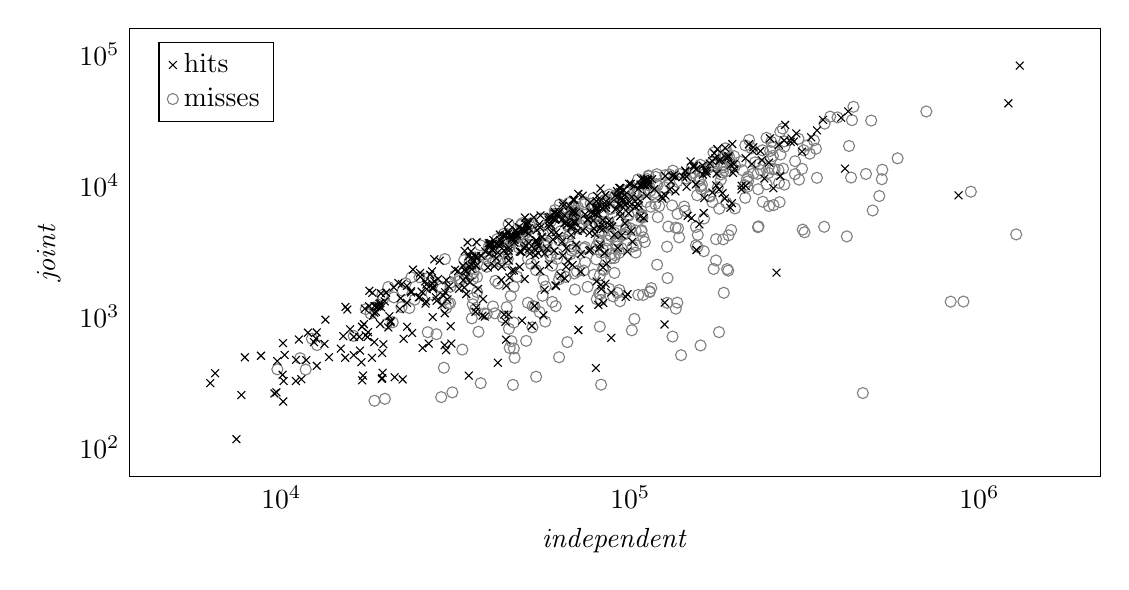
\begin{tikzpicture}
\begin{axis}[scatter/classes={x={mark=x,draw=black},o={mark=o,draw=gray}},xmode=log,ymode=log,x post scale = 1.8,ylabel=\emph{joint},xlabel=\emph{independent},tick style={draw=none},legend pos=north west,legend cell align = {left}]
\addplot[scatter,only marks,scatter src=explicit symbolic]
table[meta=label] {
x y label
151038 12468 o
38554 2768 o
188470 7353 o
68555 5931 o
117934 8242 o
129409 10502 o
22706 1783 o
43783 2597 o
22100 1173 o
90377 8310 o
24869 1983 o
29417 2731 o
71578 4989 o
34608 2582 o
16113 707 o
85683 7796 o
9738 393 o
102674 953 o
45235 3490 o
30542 1681 o
18009 1048 o
100965 781 o
184442 3865 o
179470 756 o
17457 1133 o
65990 634 o
45402 1431 o
11740 391 o
20244 1672 o
94896 7790 o
19452 1448 o
28536 1685 o
11317 478 o
26258 755 o
35151 2097 o
89916 2780 o
155711 3389 o
43856 3723 o
33402 2685 o
12653 602 o
104454 7105 o
22259 1566 o
57007 910 o
46326 895 o
53691 345 o
144662 11273 o
27818 729 o
52494 1197 o
35129 963 o
38765 1042 o
93363 1301 o
91228 3823 o
131687 7020 o
97364 4801 o
37247 308 o
45628 645 o
92056 3804 o
83449 3217 o
265592 13094 o
46584 481 o
29219 404 o
46356 567 o
44870 801 o
52407 822 o
36701 761 o
50844 1266 o
46074 299 o
82427 300 o
30893 262 o
80004 4992 o
83664 6014 o
87029 6646 o
112684 11868 o
85114 5206 o
81360 3814 o
78629 2074 o
83212 6246 o
61572 3007 o
51879 5124 o
69771 5522 o
78239 7977 o
48195 4176 o
62710 7126 o
82569 5002 o
91793 3416 o
52024 3505 o
54537 3525 o
66710 7339 o
51467 4624 o
41835 1777 o
60757 6464 o
60698 6043 o
36406 1526 o
43206 3349 o
81383 1494 o
83363 2296 o
88072 2772 o
40559 2623 o
28856 1628 o
44792 5074 o
43382 4256 o
39348 3426 o
98895 5859 o
73744 7165 o
63094 2070 o
67866 3186 o
67306 2978 o
81791 2058 o
77392 6768 o
73133 5174 o
80098 1350 o
35748 2805 o
81886 1475 o
83836 2253 o
56358 1894 o
54938 1076 o
68620 6896 o
90036 2141 o
39218 2671 o
71510 4685 o
67649 3406 o
105357 8838 o
109970 3688 o
42335 2598 o
59729 1286 o
57883 3200 o
74159 3377 o
42267 2754 o
50288 648 o
37142 3485 o
87692 6586 o
107693 5785 o
90652 3588 o
73420 2232 o
64254 3919 o
96213 4212 o
104003 3475 o
92739 3040 o
101485 3400 o
50880 2749 o
90181 2930 o
70668 6207 o
67305 5919 o
187408 19172 o
238873 18503 o
827349 1292 o
900086 1294 o
136313 1270 o
53187 1183 o
1274906 4218 o
234566 14549 o
945059 8932 o
108690 1452 o
53631 2248 o
111813 11160 o
112859 11724 o
24087 1338 o
119270 2476 o
33932 2034 o
40886 1052 o
81101 5369 o
59181 2877 o
38090 2488 o
186957 17184 o
26904 1470 o
428892 11460 o
489818 31238 o
417013 4071 o
65993 6645 o
55364 5566 o
90097 8115 o
105205 11103 o
150100 13609 o
94436 8125 o
173443 14122 o
64584 6036 o
49838 4266 o
171755 7442 o
162524 5572 o
154128 4807 o
473164 12210 o
114180 9081 o
129288 12089 o
103532 4518 o
118847 10193 o
44403 3875 o
102938 9011 o
110492 10653 o
41545 3879 o
32431 1868 o
49226 4601 o
56308 4210 o
51939 2513 o
67769 6174 o
69113 3261 o
68207 6691 o
67284 5845 o
40133 3296 o
359169 4822 o
136452 6049 o
160410 10082 o
81358 4447 o
59204 5323 o
159526 9370 o
79832 2716 o
107640 4546 o
47867 4049 o
43116 979 o
127562 1266 o
494551 6424 o
107799 5982 o
29670 1154 o
89221 1417 o
127775 1956 o
114771 1640 o
113680 1548 o
173207 2294 o
113541 1530 o
70287 2193 o
30517 1802 o
463505 259 o
28703 241 o
19797 234 o
18481 226 o
526934 13146 o
525346 11131 o
516712 8283 o
109614 9171 o
181927 12100 o
87927 2991 o
20081 878 o
206965 15142 o
120962 6949 o
171801 15041 o
82397 1331 o
29445 1343 o
20844 899 o
56423 3567 o
310420 13363 o
191148 4151 o
108885 4005 o
82440 3055 o
134806 4747 o
232851 4857 o
50200 3553 o
231194 12233 o
84388 7715 o
209581 13032 o
255846 19441 o
216377 9755 o
232352 9337 o
321278 20193 o
296172 12174 o
248513 13591 o
373695 33467 o
175891 2666 o
360118 29570 o
245526 23049 o
218781 22222 o
392254 32997 o
57527 3614 o
89805 4367 o
59648 2436 o
583110 16080 o
213273 8021 o
313753 18515 o
704713 36643 o
69072 2120 o
190772 2230 o
199733 14096 o
99986 4688 o
38765 2386 o
194448 4560 o
47893 3352 o
142591 6884 o
217350 10720 o
217601 11637 o
273872 13404 o
158662 12690 o
97816 9150 o
167742 13639 o
182763 14312 o
157092 10811 o
58910 2899 o
75392 1677 o
69349 1598 o
35420 1375 o
74204 2579 o
435582 39796 o
296448 15278 o
227529 14970 o
215616 11187 o
225223 12303 o
431474 31452 o
276192 10124 o
212807 10025 o
107454 4460 o
258993 13310 o
254989 13250 o
139718 504 o
62460 486 o
335583 22047 o
62460 1913 o
189339 2290 o
134924 1142 o
85919 3785 o
97310 4346 o
87928 4082 o
155978 4182 o
57158 1684 o
249610 6941 o
342364 11406 o
185200 1510 o
38148 1049 o
61110 1194 o
181634 11026 o
158777 9786 o
87027 4227 o
128361 4845 o
40390 1188 o
154053 3475 o
158896 598 o
252764 15906 o
269311 17165 o
326581 17434 o
96941 4606 o
48528 4971 o
36366 1993 o
35360 1920 o
95711 7749 o
176708 14629 o
132341 12940 o
66107 5010 o
175965 3877 o
179745 6628 o
48966 5133 o
222020 19202 o
21011 1392 o
30669 1813 o
107461 5918 o
155354 8394 o
257157 7057 o
266600 10429 o
26329 1961 o
44531 2729 o
125909 11946 o
117396 8794 o
148643 11517 o
73537 3294 o
12235 673 o
105733 8787 o
74222 7407 o
125085 9666 o
95014 4177 o
66332 3750 o
114419 6860 o
86869 1623 o
161849 12855 o
167418 13791 o
86978 5140 o
56025 1433 o
35859 1125 o
74833 5386 o
51384 5024 o
69415 6359 o
213423 20181 o
251463 18303 o
236344 13050 o
253266 21482 o
107320 5685 o
46075 3813 o
92275 5362 o
102115 8770 o
65292 1999 o
34974 2798 o
185938 16187 o
138402 12179 o
190285 17428 o
163919 13328 o
79020 6933 o
63158 4462 o
199339 6657 o
119646 9982 o
65148 5609 o
48250 3757 o
81498 3607 o
102502 8623 o
69561 6194 o
256165 16759 o
239458 7485 o
38967 2995 o
58297 4458 o
69255 5370 o
66252 4853 o
76948 7250 o
119017 12155 o
231968 4787 o
83043 4406 o
80042 3452 o
315376 4378 o
108223 5659 o
187464 12773 o
267634 7434 o
303094 22670 o
30443 1259 o
93028 1585 o
137937 4000 o
184101 12572 o
35330 1234 o
30103 1245 o
98754 5965 o
70030 5738 o
98219 8797 o
103552 3063 o
23569 1981 o
61609 2739 o
132139 9513 o
119779 5714 o
87027 8501 o
78202 6912 o
127372 3397 o
41033 1866 o
94328 3302 o
311651 4586 o
136013 10665 o
191214 15568 o
31448 2041 o
19616 1371 o
84537 7651 o
57220 3477 o
70722 6810 o
273243 27139 o
69191 2638 o
84830 7226 o
91239 7233 o
169153 8214 o
46316 1679 o
85275 3276 o
118153 11605 o
81735 833 o
276086 19687 o
44225 1174 o
132057 699 o
76930 5113 o
35586 2170 o
162368 3139 o
49091 4015 o
56707 3449 o
117898 7179 o
51862 4796 o
158560 11306 o
44022 3936 o
143303 6393 o
185109 13724 o
177936 9615 o
136997 4694 o
62570 3802 o
67044 4227 o
96320 6260 o
248804 12436 o
276045 21633 o
245552 10184 o
268823 25697 o
192434 16197 o
198252 16687 o
158540 14336 o
173014 17827 o
32261 1928 o
77450 5023 o
182061 13611 o
168612 8353 o
33000 556 o
45094 572 o
51348 3501 o
47391 2005 o
79002 5819 o
304192 11049 o
112867 10010 o
91786 1509 o
105369 1455 o
23259 1155 o
18471 1167 o
92265 8585 o
423110 19969 o
111071 7464 o
340073 19031 o
90377 8310 x
41379 3573 x
48751 4671 x
40212 3563 x
50319 4448 x
93474 6308 x
50137 3459 x
53724 3810 x
78678 4658 x
84331 3042 x
42175 3457 x
42767 3607 x
40068 3228 x
86868 5362 x
49665 3310 x
98785 6116 x
157707 5041 x
19438 523 x
25983 1301 x
28106 1923 x
22901 1704 x
18461 634 x
28415 2655 x
38271 993 x
42660 1886 x
48188 3122 x
6461 367 x
6255 308 x
17242 869 x
19184 872 x
12623 752 x
17025 831 x
27841 1313 x
59228 5012 x
34437 352 x
11405 330 x
42371 3819 x
43700 4136 x
39632 3509 x
34519 2412 x
41378 3562 x
12631 418 x
88705 4845 x
79659 402 x
34356 2868 x
36238 3676 x
44741 4287 x
35186 2813 x
30560 838 x
19403 332 x
21109 342 x
7434 115 x
22262 329 x
9677 262 x
17041 324 x
19440 337 x
16134 695 x
25001 2000 x
17840 1191 x
41701 441 x
37386 2891 x
30696 618 x
49381 4592 x
41694 3063 x
39047 2355 x
54847 5063 x
68324 6371 x
64750 5923 x
25809 1843 x
19507 370 x
19604 611 x
22400 672 x
13292 615 x
17865 1565 x
51094 4277 x
29469 1521 x
29135 1436 x
15455 1126 x
18224 1510 x
70946 783 x
71356 1130 x
17675 694 x
10105 623 x
8742 499 x
7680 250 x
19101 1245 x
17719 756 x
18767 1186 x
14799 565 x
26096 1611 x
38405 3125 x
33883 2009 x
36321 2772 x
35991 1082 x
36207 1166 x
33189 1885 x
15737 795 x
19765 1299 x
23538 1517 x
21854 1134 x
48170 2380 x
45719 3844 x
9728 454 x
29375 1054 x
11917 748 x
12567 674 x
33424 1657 x
7859 485 x
10152 320 x
29644 551 x
24935 1402 x
19219 1266 x
29913 1342 x
10218 506 x
13372 941 x
44026 662 x
60344 5520 x
10078 357 x
16117 504 x
15260 1179 x
18498 1195 x
80018 1845 x
26024 1748 x
16800 546 x
23815 2271 x
23514 1555 x
27447 1851 x
45733 2225 x
18183 481 x
11012 464 x
26429 618 x
11007 320 x
10121 223 x
13693 487 x
46430 2237 x
48704 3103 x
11781 462 x
154695 3205 x
176627 12278 x
37828 1353 x
22146 1762 x
20973 1664 x
44111 1709 x
44794 3169 x
96962 1404 x
46546 3841 x
19287 1493 x
33533 2270 x
35511 2669 x
52207 844 x
56764 3006 x
15039 705 x
30201 1685 x
32090 2216 x
28838 1219 x
21636 1792 x
19005 1192 x
18472 1063 x
16959 445 x
19960 1514 x
43874 908 x
20388 999 x
41248 2776 x
45716 3956 x
17444 714 x
18661 1081 x
18285 1008 x
88147 684 x
103301 6850 x
24966 2138 x
15240 482 x
17139 352 x
65788 4991 x
19338 1168 x
25877 1249 x
20563 923 x
20554 900 x
20252 821 x
55097 2213 x
53164 1199 x
61321 4366 x
11222 664 x
9554 257 x
36179 2435 x
27005 2199 x
26696 2075 x
27142 985 x
46885 4133 x
34943 3134 x
39712 3632 x
90581 6569 x
92449 7167 x
68588 7752 x
58303 4842 x
54487 3025 x
100208 10261 x
63715 3706 x
67596 4724 x
55281 5888 x
64132 6965 x
50744 5020 x
66822 7001 x
68636 5263 x
69467 5278 x
76521 7356 x
64080 7337 x
50325 4968 x
82677 5018 x
105399 9405 x
111399 10756 x
72991 8333 x
55177 4744 x
60561 6086 x
70948 8595 x
46508 3640 x
51537 3016 x
36590 1614 x
100525 4472 x
53953 4555 x
69156 5145 x
34157 3662 x
33529 3159 x
39305 3614 x
33754 2190 x
111296 8285 x
96467 5127 x
104744 7243 x
82052 9457 x
60740 6268 x
42804 2390 x
66243 2639 x
97994 3123 x
35880 2836 x
42204 3585 x
82345 1735 x
29702 1880 x
39437 3462 x
40339 3202 x
44585 4421 x
52854 5685 x
70594 4489 x
64894 1943 x
85222 7528 x
81351 3296 x
72143 2983 x
69140 7741 x
65429 2385 x
33867 1478 x
101379 3707 x
92066 3315 x
84868 1773 x
35088 2285 x
39466 3003 x
51135 3623 x
36165 2426 x
53735 3755 x
81821 3526 x
94406 4159 x
89866 4175 x
98114 1472 x
83666 1263 x
59981 3850 x
61013 1718 x
63153 2047 x
68322 2462 x
85479 2514 x
64029 2909 x
58389 2475 x
69823 6170 x
58454 5120 x
61331 5504 x
421005 36705 x
256780 9503 x
179499 9284 x
871357 8383 x
1210797 42274 x
1305007 82136 x
22930 831 x
161001 14142 x
171651 15295 x
235824 18252 x
401774 32827 x
179637 15459 x
93525 9540 x
59351 4395 x
87178 4944 x
43479 1031 x
54264 3590 x
105162 7887 x
44513 2911 x
122882 8202 x
40754 2414 x
54500 3421 x
49738 4450 x
83452 4628 x
92988 9548 x
277640 28967 x
224983 19528 x
134620 8986 x
105770 7019 x
329675 23247 x
83437 2358 x
356383 31570 x
266359 20374 x
53421 2455 x
289402 22826 x
162223 6140 x
75512 5517 x
99730 6946 x
186441 7927 x
342637 26283 x
67713 4181 x
53357 2935 x
78573 6138 x
61214 1702 x
298836 24885 x
310186 18089 x
72055 2187 x
99405 7448 x
131983 11783 x
49727 4537 x
83307 5403 x
96393 8462 x
60809 5475 x
111964 10954 x
197947 14510 x
183730 8709 x
218697 20596 x
79459 6036 x
152016 13738 x
85122 6742 x
195945 20660 x
268875 11763 x
213880 9881 x
177458 18927 x
44886 3343 x
21975 1372 x
57598 3300 x
35143 2455 x
69922 3508 x
48909 925 x
56787 1593 x
186916 19284 x
165266 12315 x
37686 1011 x
56337 1015 x
44744 1029 x
80512 6811 x
80505 6611 x
93620 8886 x
62166 6070 x
27428 2724 x
49881 5671 x
59043 5752 x
61238 5984 x
79889 6441 x
45192 4098 x
68296 6077 x
106754 5800 x
44787 5088 x
47904 4783 x
80691 6133 x
50734 5256 x
102722 9881 x
249482 14901 x
242045 11264 x
237971 15550 x
40529 3818 x
224322 18272 x
198513 13271 x
117160 9350 x
85211 7117 x
181373 15677 x
165422 12870 x
161439 12055 x
163634 12982 x
154048 10163 x
133586 12077 x
79810 6635 x
111954 11141 x
55766 4007 x
76392 4329 x
93506 5797 x
27054 1778 x
83032 6688 x
83149 6679 x
78343 5385 x
42256 4206 x
74173 5998 x
112262 10114 x
65564 5245 x
27714 1397 x
88197 1519 x
22901 1266 x
129678 9297 x
143840 12763 x
175193 16052 x
110096 10017 x
125942 11798 x
94098 7043 x
115376 11127 x
109166 11133 x
130737 10711 x
76961 6213 x
109105 10030 x
79900 6747 x
58467 5428 x
62540 6247 x
81858 7540 x
91512 9031 x
79148 4254 x
81911 4676 x
208020 9292 x
75472 5435 x
68721 6233 x
144872 9750 x
125998 8346 x
62344 4110 x
73087 4524 x
293941 21602 x
82562 1613 x
168767 14671 x
84801 8421 x
60563 3158 x
141475 11631 x
106841 9965 x
76147 3155 x
154401 13311 x
112474 10927 x
67852 4879 x
33155 2431 x
196891 12433 x
213802 16134 x
144909 11651 x
53504 3192 x
80310 8294 x
208300 9923 x
46010 4143 x
47367 4250 x
55871 4041 x
99173 10292 x
143609 12963 x
58267 5710 x
162744 7986 x
51204 4690 x
47408 4132 x
32293 1622 x
25230 1540 x
17339 1140 x
107034 10143 x
65517 3316 x
123606 7903 x
96604 7117 x
222960 14541 x
151993 14184 x
107387 11213 x
43151 4140 x
46972 4534 x
46999 4462 x
145952 5846 x
64708 5120 x
36140 2888 x
51207 3257 x
251238 22863 x
95833 9170 x
87413 7205 x
92054 8207 x
110327 10915 x
79970 7563 x
95015 7704 x
110109 10136 x
193995 14352 x
94478 8064 x
12404 634 x
125257 865 x
23691 745 x
288118 21463 x
275933 22008 x
25389 572 x
29362 600 x
31469 2264 x
149786 5629 x
27151 1627 x
27193 1668 x
125469 1269 x
80949 1220 x
16721 696 x
109297 5621 x
195372 7307 x
193416 6745 x
44023 4147 x
176283 9978 x
171783 8820 x
43418 3173 x
34724 1825 x
44811 2665 x
190647 16348 x
134557 11528 x
76798 3212 x
173885 17566 x
187879 16266 x
100980 8134 x
45053 1975 x
49790 1922 x
262195 2154 x
24734 1392 x
63616 5482 x
411952 13407 x
191096 16746 x
148748 15207 x
};
\legend{hits,misses}
\end{axis}
\end{tikzpicture}
\caption[Analogical Hits and Misses]{A scatter plot of hits and misses for analogy solution as functions of the number of jointly non-zero dimensions versus independently non-zero dimensions, with both axes scaled logarithmically.}
\label{fig:xando}
\end{figure}

So it looks like what's happening is that, as the overlap between the words involved in an analogy decreases, the expected location of the fourth point is pushed into problematic regions of the space on a dimension-by-dimension basis.  This can be visualised by once again considering the dimensional analysis of analogy illustrated in Figure~\ref{fig:histograms}.  In the case where the dimension-selecting word is the first component of the analogy (\emph{A} in \emph{A:B::C:D}), the expected location of the fourth point is actually pushed into the negative region of the dimension, where there is no information to be found.  In cases where \emph{B} or \emph{C} are the selecting words, \emph{D} would be expected to be paired with this selector, and so to have a relatively high value along the same dimension.  Overall, in these cases where, again, there is minimal co-occurrence information shared between the different input components, the fourth point is pushed into an increasingly unlikely region of a subspace, and the likelihood of a semantically plausible output decreases.  This \emph{post hoc} analysis suggests that more nuanced approaches to the dimensional selection process, for instance something like a partial application of the \textsc{zipped} technique, where there is a guarantee of some information for all input words, might be prescribed in cases where, based on frequentist features of the input, difficulty in completing an analogy is expected.

More generally, it's not particularly surprising that there is a fairly strong positive correlation between the total number of jointly non-zero dimensions and the number of independent non-zero dimensions: word-vectors with more non-zero dimensions are more likely to have an overlap with other word-vectors.  But the sharpness of definition of one boundary of this relationship is notable, even given the logarithmic scaling of the plot, with a dense clustering of both positive and negative results with a relatively high overlap compared to relatively low forming a distinct ridge along the upper left perimeter of the distribution.  The implication here is a long tail of increasingly disconnected word sets drifting off to the lower right hand of the plot: this could mean that there are mismatches between the co-occurrence profiles of the input terms as well as the relative frequencies of the terms.  One quite plausible hypothesis, which is certainly open to future empirical exploration, is that the nature of the distribution illustrated here is peculiar to analogy, and that, if random trios of words were selected, the lower right region of the plot would be more filled in as we discovered more instances of words with a wide range of co-occurrence features but relatively little overlap between one another, corresponding to conceptual disparity.

\section{A Note on the Data} \label{sec:datanote}
It must be mentioned that the data that has been analysed in this chapter is of a very specific character.  The analogies put together by the team at Google are populated by a high percentage of proper names, specifically place names and also currencies, demonyms, and the like.  This belies a particular view of language and indeed cognition which is at odds with the premise motivating the methodology described in this thesis, as outlined at the beginning of Chapter~\ref{chap:theory}.  Proper names are, as \cite{Russell1905} has pointed out, particular kinds of words with peculiar denotational properties in that they refer to specific and unique entities or correspondingly specific classes of entities.  This is not to say that they do not admit ambiguity -- \emph{Paris} is the name of, among other things, a classical character, and \emph{Berlin} the name of a 1980s new wave band -- but there tends to be a certain clarity of intent when these types of words are used.  The types of analogies found in this data are exemplary of cases where language coalesces into a relatively stable conceptual representation, and, notwithstanding instances of polysemy, it is arguably not particularly surprising that these relationships emerge as commensurable directions in a likewise stable representational space.

Furthermore, it is telling that the designers of the dataset have chosen to refer to the variety of analogy typified by \emph{Denmark:Danish :: China:Chinese} as \emph{syntactic}, whereas the relationships denoted by \emph{grandfather:grandmother :: grandson:granddaughter} is considered \emph{semantic}.  Both of these examples exhibit conceptual relationship that to a certain extent map to morphological features of the representations involved, and so exemplify some of the characteristics of conceptual schemas described in \citepos{Langacker1991} cognitive grammar.  It seems like the designers of this dataset resorted to some instinctive assumptions about the categorical nature of concepts in their selections, ultimately landing on classifications which are pointedly unambiguous.  This is well motivated, and the data has provided a very useful tool for exploring the geometry of contextualised distributional semantic subspaces, but there is also an element of conceptual absolutism at play and a corresponding drift from the looseness and ambiguity that overwhelmingly characterise natural language as it is actual used by humans.  We might reasonably conjecture that these types of conceptual relationships are particularly conducive to the geometry of static semantic spaces such as those generated by \texttt{word2vec}.

\cite{Linzen2016} has made some very interesting observations regarding the way that analogical geometry actually plays out in \texttt{word2vec} models.  For one thing, it turns out that the parallelograms expected to emerge in analogical mappings are in fact, in the case of the data tested here, elongated to such an extent that they are effectively lines and the models would usually return one of the input terms if it weren't for a systematic constraint prohibiting this.  This supports the observation made regarding the conceptual compartmentalisation noted in Figure~\ref{fig:inspace}, but it also suggests that the types of analogy being analysed here involve pairs of words that, in the static spaces generated by the neural networks of the skip-gram and CBoW methods, are clustered into very distinct semantic regions of static spaces.  A related finding was that in a number of cases, the expected completions to analogies were so proximate to one of the input words that a simple nearest neighbour approach based on a single input would return the specified output.  This is particularly the case in analogies involving demonyms and capital cities, where the propensity for words related along these conceptual axes to be observed in similar sentential contexts is presumably so high as to cause the models to push their vectors into virtual collocation.

In order to explore the performance of distributional semantic models as they move outside the boundaries of analogies between well defined conceptual domains, I experiment with a small, curated set of analogies that are designed to transgress in various ways the type of conceptual boundaries inherent in the data explored in the previous section, outlined in Table~\ref{tab:transgressions}.  In some cases -- for instance, mappings between \textsc{instruments} and \textsc{instrumental components}, or, with the exception of the \textsc{indy} technique, the metaphor between \textsc{seasons} and \textsc{moods} borrowed from \emph{Richard III} -- there is at least broad agreement between the semantic space making techniques.  It is only the \textsc{joint} method, however, that discovers immediately logical mappings for projections from \textsc{substance} to \textsc{temperature}; likewise in the case of the mapping from \textsc{material} to \textsc{product}, it is the \textsc{joint} method that moves furthest away from the input itself, with the other three methods returning either versions of \emph{words} or the slightly removed \emph{phrases}.  Similarly with the more metaphoric analogies towards the bottom of the table, the \textsc{joint} technique generates certainly the most provocative, if not always entirely logical, outputs.

\begin{table}
\centering
\begin{tabular}{l|llll}
\hline
input & \textsc{joint} & \textsc{indy} & \textsc{SG} & \textsc{CBoW} \\
\hline
\emph{stool, sofa, motorcycle} & car & bike & motorbike & motorbike \\
\emph{surgeon, butcher, scalpel} & knife & butchers & knife & butchers \\
\emph{key, piano, string} & violin & cello & cello & violin \\
\emph{fire, ice, hot} & cold & topped & bubbling & hockey \\
\emph{paint, words, picture} & speech & word & phrases & word \\
\emph{discontent, winter, glorious} & summer & olympics & summer & autumn \\
\emph{theater, world, actor} & commentator & won & medallist & medallist \\
\emph{candle, life, wind} & disturbance & winds & lives & lives \\
\emph{sleep, dream, death} & marriage & murder & fathers & untimely \\
\emph{beloved, lover, empire} & rule & empires & empires & empires \\
\hline
\end{tabular}
\caption[Transgressive Analogies]{Results for a few different models, with 5x5 word windows and 200 dimensional spaces, for completing a small set of analogies spanning various conceptual domains.}
\label{tab:transgressions}
\end{table}

Returning again to the elongated geometries of Figure~\ref{fig:inspace} and the insight of \cite{Linzen2016}, the static methods, along with the \textsc{indy} technique, seem to struggle to make the transgressive leaps necessary to offer creative and compelling solutions to analogies with less overtly categorical interpretations.  In the case of the static methods associated with \texttt{word2vec}, it must be recalled that the spatial features defining semantic relationships in the consequent models are fixed: while they seem to capture well the sort of general or encyclopaedic knowledge inherent in the dataset generated by \cite{MikolovEA2013} to test them, their performance deteriorates when it comes to framing semantics in terms of the \emph{ad hoc} conceptualisations that come up in the course of a dynamic engagement with a complex environment.\footnote{A perhaps slightly harsh critique would be that these models are trained on corpora like Wikipedia and then in the end are best suited to telling us precisely the kinds of things we could look up in Wikipedia, anyway.}  The poor performance of the \textsc{indy} technique on these examples suggests that this method is also possibly better suited for handling stable lexical representations; the strong results in Tables~\ref{tab:solutions} may, in fact, be an artefact of this property of these subspaces, and this invites further research into subspace selection techniques.

In the end, none of the geometric semantic modelling techniques surveyed here seem particularly well suited for completing conceptually sophisticated analogies, or for that matter for extrapolating metaphor by way of analogical inference.  The problem is that the conceptual geometries generated, certainly in the case of the static models, tend to be quite categorical in the way that they group lexical semantic representations.  This effect is arguably less evident in the case of the context sensitive methodology, particular applying the \textsc{joint} technique, but a dimension-by-dimension analysis of co-occurrence counts still definitely leaves something to be desired in terms of the spaces it maps.  We can see flashes of the deeply interpretable conceptual geometry described by \cite{Gardenfors2000} and \cite{Widdows2004}, but there is a long way to go before we could talk about extracting a rich intensional network from directions and regions within these spaces.  On the other hand, the results modelling analogies given full information of all four points described in Table~\ref{tab:knowns}, and indeed modelling arbitrarily constructed relationships, as reported in Table~\ref{tab:fakes}, suggest that there is likely to be \emph{some} subspace in which any given parallelogram of analogical relationships can be constructed.  The \textsc{joint} technique for subspace projection seems to have the best chance of generating geometries with at least some degree of semantic productivity---and this makes sense, since this technique takes into account information about all inputs along every dimension, guaranteeing that the shapes associated with analogy or for that matter any other semantic phenomenon will be fully in the projected subspace rather than anchored along the corners due to the sparsity of the vectors of their vertices.

It is worth recalling, as mentioned in Chapter~\ref{sec:twomeasures}, that the dimensions that compose a subspace cannot be interpreted in a one-by-one way; rather, they collectively constitute a context in which semantic relationships emerge.  Along the same lines, I will suggest that the conceptual geometry which affords analogy, and the attendant potential for, for instance, metaphor making, is not always open to instant interpretation in terms of the informational transfer at play in the linguistic construction.  This supposition is in line with the relevance theoretical approach to metaphor discussed originally in Chapter~\ref{sec:words} and again in the context of my own methodology in Chapter~\ref{sec:intercomp}.  One way forward under this premise is to move away from the analytic assessment of the independent situations of word-vectors on individual dimensions, and instead to take a more holistic (and also computationally expensive) view of how overall geometries emerge as subspaces are built up.  So, for instance, we might look for trios of analogical input that constellate as right-angular, isometric triangles over the run of many dimensions, guaranteeing a space that has a more nuanced co-occurrence profile for input and output and so offers richer semantic information about the analogy \citep[a similar idea is discussed in][]{McGregorEA2016}.


\chapter{Conclusion}
Looking back on the work presented here, \emph{perspective} seems like a good word to apply to various aspects of my research.  First of all, the methodology that I have developed is rooted in a theoretical perspective, or maybe more a perspective on a theoretical domain within the study of language and cognition.  I prefer to call this a perspective rather than, for instance, a \emph{stance} because I have at least attempted to treat the theoretical background surveyed in Chapter~\ref{chap:background} and then applied to the notion of semantic models in Chapter~\ref{chap:theory} as a facilitator rather than as a constraint on the empirical work that follows.  Then, in the approach to lexical semantic modelling presented as an idea in Chapter~\ref{chap:theory} and developed as a computational implementation in Chapter~\ref{chap:method}, I have put forward a methodology rooted in the notion that there is much to be gained from considering semantic information in terms of contextual perspectives taken on data.

In the experiments on the quantitative modelling of semantic phenomena described in Chapters~\ref{chap:relsim} and \ref{chap:figurative}, the geometric interpretation of the statistical features used to learn models for rating or identifying these phenomena provides traction for probabilistic analysis according to the mathematical provisions of the methodology, and, in turn, speculation about the cognitive correlates of frequentist observations about language use.  One of the stipulations of my technical approach has been that the operations of a quantitative model should continuously submit themselves to interpretative analysis, offering once again a perspective on the way that observable and indeed countable characteristics of word use build up into an emergent model of semantic relationships.  By maintaining a connection between the features submitted to machine learning processes and the underlying observations of large scale data, I have sought to demonstrate how we can treat the supervised learning of models of semantic phenomena as not only a task-completing mechanism, but also an enabler of subsequent theoretical insight into the nature of language use.

The experiments on analogy modelling and completion in Chapter~\ref{chap:analogy} offer an opportunity to explore my methodology's capacity for generating semantically productive geometric lexical representations in an unsupervised manner.  The categorical analysis of a couple of my techniques for subspace projection on analogy completion tasks provides insight into the way that data-driven semantic space type models both succeed and fail at delineating the sub-conceptual regionalism crucial to a productive semantic space.  This type of forthright analysis, continually seeking to return to the data itself and the way that the dynamics of representations are tied to the computation of observed language use, provides the basis for a more qualitative assessment of the functioning of a model of intricately interactive units, often leading to challenges directed at the data used to evaluate a methodology in the first place.  Ultimately, my geometric approach opens itself up to the potential for a radical approach to semantic modelling, not taking for granted the supervenience of the lexicon upon a well defined framework of composite conceptual representations; instead, with a context sensitive approach to distributional semantics, we can afford to imagine lexical-conceptual relationships as abstract but nonetheless graspable structures perpetually emerging from the dynamic between an agent and an environment, and the lexicon itself as a facility wrapped up with conceptualisation rather than a symptom of it.

The question which motivated this research was whether data about word co-occurrences could, through the application of statistical analysis and by way of geometrically situated lexical representations, be translated into semantically useful information.  My hypothesis, that a routine of contextualisation taking the form of online projections -- perspectives -- from the statistical space, has been supported, inasmuch as results ranging from competitive to outstanding have been returned on a variety of tasks.  Moreover, the nature of my methodology has provided the basis for post-experimental analysis of the way that its representations are extrapolated from large scale data, and I consider this to be an achievement of at least as much value as the task-completing capacity of the methodology itself.  This thesis has been laced throughout with theoretical conjecture, and it is the interpretability of the operation of my techniques which permits a continual return to the philosophical assumptions and implications of my approach.  In these final few pages, I will seek to summarise the empirical results obtained over the last three chapters, consider how these overall results might point the way towards productive future work, and then finally reflect on the philosophical ramifications of my research.

\section{Summary}
Overall, my methodology has proved to be often competitive and occasionally outstanding in its performance on a handful of tasks covering a range of semantic phenomena.  The results on ranking relatedness and similarity indicate an approach that is at least in line with other recent work in the field, some of which imposes considerably more in the way of heuristics and pre-formulated information about the conceptual referents of words than my technique does.  While the results on similarity are, like with other distributional semantic models applied to the SimLex dataset, substantially worse than the relatedness results, the comparison between the feature weights learned by linear models for addressing each phenomenon reveals interesting differences between the way that semantics play out in terms of statistical geometry, painting a picture of the way that a single analytic process might, in contextualised subspaces, provide a basis for the analysis of multiple axes of conceptual relationships between input terms.  In the end one of the most interesting outcomes of the experiments analysed in Chapter~\ref{chap:relsim} is the idea that there could be relatively blunt statistical features such as word frequency or co-occurrence dimension variance that present semantic signals.  In this respect my model could prove to be a useful tool for discovering quantitative features of language use which yield productive theoretical insights.

The results on metaphor classification are exceptionally strong, suggesting that contextualisation plays a significant role in identifying the degree to which a potentially compositional relationship between words can be analysed in terms of a transfer of information between conceptual domains.  Experiments with learning a model for graded ratings of metaphor from data annotated with merely binary tags suggest that a geometric approach aptly frames metaphor as a spectrum rather than as a sharply defined phenomenon, and it is particularly interesting to note that the movement from literal to metaphoric language is marked by what appear to be stages of statistical shifts rather than a single smooth progression of geometric features.  Results on coercion classification are not as strong as the metaphor results; while this may to a certain extent be a product of the data itself, the balance of which makes coercion identification more difficult, the accuracy scores for the best performing models and a comparison with baselines and previous work on this dataset also paint a picture of a phenomenon that proves to be more elusive for my methodology.  Furthermore, the geometric analysis of coercion offer less in terms of a clear-cut analysis of the co-occurrence tendencies that characterise type shifting.

There is, of course, a close, and perhaps at times even ambiguous, relationship between coercion and metaphor: the interpretation of each phenomenon requires some allowance for lexical looseness combined with a step of contextualisation to refocus a word that has been lured out of what might be seen as its native lexical habitat.  The difference is perhaps a matter of the nature of the underlying conceptual schemes implicated specifically in the interpretation of each of these distinctly non-literal phenomena, with the type shifting of coercion lending itself more readily to a hierarchical scheme of conceptual classes.  One way of putting this would be that, where the interpretation of metaphor seems to involve determining a context in which the conceptual deracination of a word's denotation can be understood in terms of an intensional transfer between domains, coercion interpretation comes across as more of a determination of the level of abstraction on which to consider the relationship between, for instance, a predicate and an argument.  Among other things, data involving scoring rather than just classifying potential instances of coercion would offer insight into not only the operation of my methodology but also the way that humans cognitively approach this phenomenon.

Results on analogy completion are noteworthy, if not quite on par with the remarkable outcomes of the \texttt{word2vec} techniques, for which the data I use was originally designed.  It is in the case of the work on analogy that my methodology comes closest to empirically returning to its G\"{a}rdenforsian theoretical roots, with subspaces characterised by conceptual regions and directions representing general semantic correspondences.  Analogy stands out as something of a special case in the research presented here, in that, among other things, the geometric mechanism targeting analogy completion is entirely unsupervised: the hypothesis tested is that analogies should simply play out as predictable geometric configurations in an appropriately contextualised subspace.  The geometry specified, in line with other models, is that of the parallelogram, suggesting a conceptual coordination in terms of orientation and distance in a semantic space.  An analysis of optimal subspaces, though, indicates that there might be even more specific types of polygons implicated in the mapping of analogy: rectangles or squares with a certain orientation in relation to the edges of a positively valued subspace, for instance, might be even more strongly associated with the intensional coordination at play in analogy.  Choosing dimensions that are collectively best for facilitating these properties poses a potentially hard computational problem, however, as the angles and balances of side lengths of polygons are products of the overall situation of the shapes' vertices and cannot even be approximated based on a dimension-by-dimension analysis.

\section{Outlook}
The work described in this thesis has involved the extrapolation of contextual semantic models from digitised textual data through the application of information processing procedures interacting at many different stages along the passage from raw data to semantic information.  This methodology can be understood in terms of the parameters which correspond to these stages, which can be summarised as follows:

\begin{description}
\item[Data] The corpus selected for building a base space of co-occurrence statistics and the data cleaning procedures applied to this corpus;

\item[Word Counting] The method used for tabulating co-occurrence counts, which in the work described here has involved simply seeing how close words are to one another in a sentence but could also be calculated in terms of, for instance, distance along the branches of a dependency tree;

\item[Statistical Processing] The function applied to word frequencies and co-occurrence counts in order to derive the elements of a base space for subsequent contextual projection;

\item[Subspace Selection] The techniques, including the choice of contextualising input, for applying a statistical analysis of word-vectors to the selection of a set of dimensions for subsequent geometric semantic analysis;

\item[Geometry] The measures and mappings used to extrapolate semantic information from the situation of word-vectors in a contextualised subspace.
\end{description}

\noindent The research presented here has offered a sampling of possible combinations of these parameters; my intent has been to focus on higher level issues of theoretical grounding and philosophical import, in the context of a rigorous but also broad survey of my methodology's application to a handful of established natural language processing tasks.  This means that, to the extent that the results returned on various datasets are good enough to motivate future research with context sensitive distributional semantic models, there is already a considerable amount of work that can be done simply by way of exploring the parameter space of the methodology as it stands.  So for instance the type of language found in Wikipedia, which has particular, arguably even peculiar characteristics in terms of vocabulary, idiomaticity (or lack thereof), sentence length, and so forth may not be best suited for building dimensions that are amenable to contextualisation.  Likewise there might be more effective techniques for subspace selection, involving for instance an analysis of the relationship between word-vectors along a dimension, or even just an analysis of general statistical characteristic of dimensions such as mean and variance.

A particularly interesting topic for future research is the question of how best to translate word-counts into informative statistics about co-occurrence relationships.  The application of an information theoretical metric is attested in the literature and has proven fairly effective for the tasks described here, affording a mechanism for translating probabilities into geometric features, but there are a variety of other functions that can be applied to word-counts, as well.  Should logarithmic dimensions, for instance, be weighted by the probability of a joint occurrence of their correlates, allowing for a sort of entropic analysis of a dimension's distribution?  And does the warping factor of the smoothing constant and the shifting of ratios of probabilities prior to taking logarithms perhaps have an adverse effect on conceptual geometry?  The removal of these constants, which were introduced to enable the dimension selection process, may allow word-vectors to fall into an even more semantically interpretable geometry.  And if values along dimensions are constructed as probability distributions, then this opens them up to a potentially productive analysis in terms of probabilistic moments, providing another set of features that can possibly be mapped to the semantic character of subspaces.  There is even scope for applying a kind of reverse subspace selection procedure, seeking to induce, given a subspace which we know to be in some sense semantically productive, the kind of word-vectors which would indicate such a subspace.

In terms of analysing the geometry of subspaces, it may be worthwhile to consider any of these phenomena in terms of proximity by way of relative ranking within subspaces, rather than in terms of absolute geometric measures.  So, for instance, the similarity between pairs of words may be more accurately mapped as a function of the number of other word-vectors closer to either input word-vector, within a contextualised subspace, than either word is to the other: this could go some way towards addressing the issues of framing raised in Chapter~\ref{sec:frames}.  A similar measure could be applied to words' relative distance, in terms of rank rather than norm, from the origin.  And likewise, ranking measures could be applied to generic points of the space; in fact, this relativistic approach might serve to mitigate the influence of outliers in terms of maximum and mean vectors, lessening the impact of values that are simply aberrantly far from anything else by virtue of low independent frequencies combined with high joint frequencies.

More ambitiously, we might consider other ways of modelling the lattice of contextual subspaces itself.  The projections afforded by one of the base spaces that my methodology generates can, as outlined in Chapter~\ref{sec:litdims}, be understood as a power set of contexts, and so a discrete structure that can be thought of as an unweighted network of possible subspaces.  If we consider the relationships between dimensions, however, and in particular establish a metric of distance between dimensions, then the immense space of possible projections becomes a smooth manifold, a continuous space of at least suppositional positions within a lattice of unbounded subspaces.  This construct would have powerful mathematical attributes, potentially allowing for the modelling of semantic relationships in terms of differentiable movements across contexts rather than just as static relationships within dynamically selected but discrete subspaces, opening my approach up to coordination with the promising techniques of the relatively new field of information geometry.

Finally, the nature of the tasks towards which my methodology can be applied, and the corresponding evaluation of performance on these tasks, deserves further consideration.  The type of datasets used here, which are fairly typical of the approach in natural language processing in general, seek to facilitate a quantitative evaluation of computational models.  This is well motivated, and the data used for exploring relatedness \citep{FinkelsteinEA2002} and similarity \citep{HillEA2015} are characterised by thoughtful consideration of some of the clinical, psychological background by way of word association studies, while the coercion data \citep{PustejovskyEA2010} is thoroughly grounded in the theoretical linguistic literature and, in its provision of sentential context, can be used a source to explore further degrees of contextualisation.  \revJB{1}{Metaphor is a likewise widely studied linguistic phenomenon, and the ongoing interest in the topic has resulted in a wealth of resources for evaluating computational models not just for classifying but also for interpreting and generating metaphor.  The work described in Chapter~\ref{sec:metperiment} could be expanded with further exploration of ways in which the analysis of, for instance, the dimensions involved in the identification of metaphor might lend itself to the extraction of a corresponding interpretation of a metaphor, or of how subspaces might be discovered in which contextual input leads to the generation of a potentially novel metaphor discoverable in the geometric relationships between known target words and candidate source words.}

\revAK{22}{It is likewise worth considering how my methodology might be applied to a wider range of natural language processing problems, including those with a more overtly practical component.  I have not directly evaluated the capacity of context sensitive distributional semantic subspaces to capture polysemy, but it seems reasonable to conjecture that we might achieve positive results, as context is in some regard precisely the mechanism for resolving ambiguous word senses.  Successful application of my techniques in this domain could lead on to work on such practical objectives as contextualised search and question answering.  There might likewise be an application for my methodology in the domain of entity resolution, where contextualised semantic representations could provide vital evidence to link otherwise misaligned data that properly belongs to the same record.  There could be ways in which a more general manifestation of my techniques for subspaces projection and the analysis of statistical geometry could enhance existing techniques in topic modelling that are to some extent conversant with distributional semantic techniques: latent Dirichlet allocation} \cite{BleiEA2003}, \revAK{22}{for instance, might be augmented with a contextually specified vocabulary indicating the words that become the basis for generating topics.  We might even imagine a corollary application to network analysis, where edges in a graph could be selectively activated to generate contextualised perspectives on a very large system of relationships, though this is beginning to move away somewhat from the underlying linguistic component of my methodology.}

The task-oriented approach to evaluative computational linguistic systems inherent in these datasets has proved a valuable way of feeling out the capabilities and limitations of my methodology, and comparison to other approaches that have been applied to the same data likewise serves as a useful way of understanding where a contextual paradigm works and where it might be improved.  Nonetheless, any dataset configured in terms of decontextualised samples of language and scores is going to have biases built into it, from the way in which representative language instances are chosen to the decisions about what constitutes a correct or adequate output.  I maintain that a more qualitative approach to computational linguistics, orientated towards processing heterogeneous inputs and then subjected to a subsequent analysis in terms of the impact of outcomes rather than simply the scores of outputs will provide the basis for a much more thorough understanding of what the type of model I've described in this thesis might be able to do.  With this in mind, I propose that the digital humanities are an appropriate target domain for the development of my methodology.  A particular appeal of the humanities is the inherent appreciation of critical perspectives on data: rather than framing semantic modelling in terms of correct solutions to tasks and corresponding scores, there is a notion that any semantic commitment is wrapped up in a perspective on the world.  The connection between this philosophical stance and my methodology should now be obvious: we can begin to imagine how, rather than providing a singular interpretation of linguistic data, a contextual approach to distributional semantics might offer a proliferation of different approaches that come equipped, by way of the interpretability of literal spaces of co-occurrence dimensions, with a mechanism for extrapolating not just an \emph{explanandum} but also an \emph{explanans} of model output.

There is a movement afoot to take the digital humanities beyond its foundation in textual studies, towards a more interpretive approach to handling on a massive scale the resources with which humanists have traditionally worked \citep[see][for an interesting discussion]{AllingtonEA2016}.  \cite{Moretti2013} has offered one version of a general framework for such an undertaking, and more concretely empirical work has already been initiated by \cite{HopeEA2010} and \cite{Ahnert2015}, with \citeauthor{HopeEA2010} in particular proposing a mechanism for interpreting a large scale digitised canon explicitly using the techniques of distributional semantics.  In addition to providing a tool for computationally establishing critical semantic perspectives, I propose that the interpretable nature of my methodology can offer further value by tying the output of a computational process directly to passages in the underlying data.  So, for instance, when it turns out that a particular set of dimensions is best suited for mapping out an analogical interpretation of language use in a work of literature, a contextual model would be able to refer a scholar back to the actual instances of co-occurrences between the words being targeted and the dimensions specified, offering an opportunity to discover unexpected concordances across a potentially vast corpus.

\revAK{22}{Another target domain for applications of my methodology is cognitive science: much of the theory that has motivated my approach has been inspired by work in this active field, and so it seems natural to consider ways in which the further development of my approach might in turn inform further theoretical and practical research into the nature of cognitive agents.  One potential point of contact is the idea, mooted by} \cite{Barsalou2008}, \rev{that statistical aspects of the way that agents in the world encounter language can play a role in the construction of semantic representations.  The techniques outlined in Section~\ref{sec:finding} for discovering subspaces for the productive mapping of known analogies, which are in effect a kind of reverse engineering of vector spaces with statistical properties that correspond to pre-established semantic expectations, point towards a more general set of approaches by which we might consider building cognitively expressive geometries and then exploring the ways in which the features of those subspaces map to stances on the observation of language in use.  Such an approach could be applied to cognitive models involving conceptual spaces} \citep{Gardenfors2000}, \rev{conceptual blending} \citep{FauconnierEA1998}, \rev{and image schemas} \citep{Lakoff1987}, \rev{each of which in its way permits a degree of spatial interpretation.  In a particularly ambitious interpretation of this proposal, we might conceive of bespoke contextualised subspaces as hypothesis engines, providing a basis for revealing potentially unexpected statistical correlates which would offer themselves up for interpretation in terms of the way that language is actually used.  This, in turn, could become the basis for productive work in modelling language acquisition in the mode of} \cite{RaczasekLeonardiEA2018}, \rev{examining how representations are forged in an environmental situation rather than how abstract symbols are arbitrarily assigned to things in the world.}

\section{Direct Encounters with Meaning}
At the beginning of Chapter~\ref{chap:analogy}, I described analogy as a kind of semantic meta-phenomenon, offering a basis for the analysis of constituent words in terms of a variety of different forms of meaningfulness.  This is because, given an analogical alignment between two pairs of words, there is presumably some aspect of conceptual correspondence along both of the axes of parallelism.  Actually knowing the nature of this correspondence, however -- actually having the meaning, the intention -- is not necessarily a component of the analogical construct, and in the end there is arguably a sort of Chinese Room \citep{Searle1980} quality to having a well-formed but perhaps poorly understood analogy.  This gets back to a question raised at the very beginning of Chapter~\ref{chap:intro}: what can we really know about words from the outside, so to speak, just in terms of how they interact with the world that they are in?  If we have just one piece of information, that \emph{A:B::C:D}, we know nothing about what any of those components denote, and almost nothing about \emph{how} they denote, by way of their semiotic contingencies and constraints, their structure on whatever level of abstraction.  But if we can patch together enough instances of such analogies, cobbling one analogy to the next by matching one edge to another, can we eventually cash out the looming construct of hinged inferences to get something like meaningfulness?  In fact, in the end, do we really ever have anything else to work with in our pursuit of meaning?

In the end, it may actually be better to think of analogy and other attendant semantic phenomena as things that can be modelled without committing to any particular interpretation.  Such an approach seems truer to the pragmatic commitment to extemporaneous lexical specification: lexemes present themselves, just like any other object, however concrete or abstract, in the \emph{umwelt} of a cognitive agent, as perceptual opportunities for action, in the specific but perhaps not special case of language as an opportunity for meaning making.  So where does a distributional semantic approach get us?  Word frequency is not a thing that is directly perceived: though I could make an informed guess, I do not actually have a sense of how often I've encountered the word \emph{the} recently, versus the word \emph{thundercloud}, versus the word \emph{fulgurate}, and even if I did have this information it would seem far removed from the way those words each inform and evoke.  Meaning, on the other hand, is directly perceived: even on the abstract level of non-iconic, highly symbolic language, there is ``the familiar physiognomy of a word, the feeling that it has taken up its meaning into itself,'' \citep[][p. 218]{Wittgenstein1953}.

What I finally claim that my contextual, geometric, interpretable take on distributional semantics points towards is pushing language into the domain of the perceivable, divesting it of the livery of its sometimes exceptional status as the intransigent medium of philosophy, shorting the circuit of language about concepts, concepts of language, and, eventually, the recursion of language about how language is about things.  Instead, in the statistically grounded geometry of a fleeting contextual semantic space, we have a chance to simply grasp at a structure with length and distance, making meaning in the same way that we might pick up a shoe to smash a fly or flap a newspaper to fan away smoke, just by applying what our situation in our environment affords us.  Under this regime, things like metaphors arise not as a consequence of computations about information transfer or even necessarily resolution of choices about optimal informational import, but simply as chance encounters with the possibilities of words as implements of conceptualisation and communication, conveying as much about how we mean as what we mean.  There are, of course, issues of supervenience and cognitive plausibility here, and I would be remiss to try to suggest that there is any reason to suspect isomorphism between my methodology and, for instance, neurological structures or psychological constructs.  All the same, on a certain level of abstraction, my approach provides access to meaning as something that is in the world in the form of a construct in an abstract space, that arises through contact with the ongoing situation in an environment, and that can be mapped back to a situation in a resource that is real and graspable.

What I am ultimately seeking to set up here is the groundwork for the application of computational techniques to phenomenologically oriented cognitive models.  This is why I have attempted to make my methodology conversant with, for instance, \citepos{Davidson1978} theory of metaphor, which is in the end about the way that language gets outside of the portage of propositions about situations in the world and into the actual fabric of the experience of existing.  If the phenomenal experience of reality -- the quality of perceiving and knowing in a world of objects and processes -- is, as \cite{Clark2016} puts it, \emph{controlled hallucination}, then words too are a layer of the veridical delusion, playing their part in the tumult of uncountable instances of tiny resolutions of uncertainty that ineffably works its way into the peculiar intentionality of being in the world.  In this work, I have sought to take words seriously as material evidence in the hunt for some sort of insight into the conditions under which meaning comes about, and I hope that my methodology, with its sensitivity to theoretical considerations and its mechanism for potentially unlimited semantic productivity, can serve as another implement in the resolution of these very hard questions.


\lhead{\emph{References}}
%\bibliographystyle{apalike}[doi]
%\bibliographystyle{chicago}
%\bibliographystyle{apa}[doi]
\bibliographystyle{apacite}
\bibliography{Mega.bib}

% Start the appendix (inc. author's publications)
\begin{appendix}
%\chapter{Author's publications}

% publications goes here

\subsection*{Journal papers}
\begin{enumerate}
  \item \textbf{Y. Gao}, X. Chen, Z. Ying and C. G. Parini, ``Design and Performance
Investigation of a Dual-element PIFA Array at 2.5 GHz for MIMO Terminals," \emph{IEEE Trans. on
Antennas and Propagation}. (Revising)

\end{enumerate}


\subsection*{Conference papers}


\begin{enumerate}
  \item \textbf{Y. Gao}, X. Chen, Z. Ying and C. G. Parini , ``Further Investigation of a
Dual-Element Diversity PIFA for MIMO Applications at 2.5 GHz Band," \emph{IEEE International
Symposium on Antennas and Propagation (AP-S)} , Honolulu, Hawaii, USA  June, 2007. (Accepted)
    
\end{enumerate}

\subsection*{Project report}
\begin{enumerate}
  \item X. Chen and \textbf{Y. Gao}, ``Final Report on Modelling of Difficult Environments,"
  Galileo Advance Concept project final report (GAC/EUT/DT/219), 9th June - 31 October 2007.
  
\end{enumerate}



\renewcommand{\thefigure}{B.\arabic{figure}}
\chapter{Solutions for the Examples in Chapter 2}
\label{examples_solutions}
\section{Example 1: Antenna Spacing Effect}

\textbf{Step 1:} Get the $H_{norm}H_{norm}^\dagger$, set $2{\pi}R/\lambda={\omega}_1$ and
$2{\pi}(\overline{R})/\lambda={\omega}_2$ ($\lambda$ is the wavelength), so
\begin{equation}
H_{norm} = \frac{1}{\sqrt 2 }\left( {{\begin{array}{*{20}c}
 {e^{ - j\omega _1 }} \hfill & {e^{ - j\omega _2 }} \hfill \\
 {e^{ - j\omega _2 }} \hfill & {e^{ - j\omega _1 }} \hfill \\
\end{array} }} \right)
\end{equation}
Note: $H_{norm}^\dagger=(\overline{H_{norm}})^T$ and $e^{j\theta}=cos\theta +jsin\theta$
\begin{equation}
\begin{array}{l}
 H_{norm}H_{norm}^\dagger = \frac{1}{2}\left( {{\begin{array}{*{20}c}
 {e^{ - j\omega _1 }} \hfill & {e^{ - j\omega _2 }} \hfill \\
 {e^{ - j\omega _2 }} \hfill & {e^{ - j\omega _1 }} \hfill \\
\end{array} }} \right)\left( {{\begin{array}{*{20}c}
 {e^{j\omega _1 }} \hfill & {e^{j\omega _2 }} \hfill \\
 {e^{j\omega _2 }} \hfill & {e^{j\omega _1 }} \hfill \\
\end{array} }} \right) \\
 = \frac{1}{2}\left( {{\begin{array}{*{20}c}
 {1 + 1} \hfill & {e^{ - j(\omega _1 - \omega _2 )} + e^{ - j(\omega _1 -
\omega _2 )}} \hfill \\
 {e^{ - j(\omega _1 - \omega _2 )} + e^{ - j(\omega _1 - \omega _2 )}}
\hfill & {1 + 1} \hfill \\
\end{array} }} \right) \\
 = \left( {{\begin{array}{*{20}c}
 1 \hfill & {\cos (\omega _1 - \omega _2 )} \hfill \\
 {\cos (\omega _1 - \omega _2 )} \hfill & 1 \hfill \\
\end{array} }} \right) \\
 \end{array}
\end{equation}
\textbf{Step 2:} Get the eigenvalue of $H_{norm}H_{norm}^\dagger$, here set $\lambda$ as
eigenvalue, then,
\begin{equation}
\left( {{\begin{array}{*{20}c}
 {1 - \lambda } \hfill & {\cos (\omega _1 - \omega _2 )} \hfill \\
 {\cos (\omega _1 - \omega _2 )} \hfill & {1 - \lambda } \hfill \\
\end{array} }} \right) = 0
\end{equation}
and $\omega_1-\omega_2=2{\pi}R/\lambda-2{\pi}(\overline{R})/\lambda=-54^o$, so
$\lambda=1{\pm}cos(\omega_1-\omega_2){\approx}1{\pm}0.59$. Hence, $\lambda_1=1.59$ and
$\lambda_2=0.41$.





\end{appendix}

\end{document}
% That's all of it!
